%
% 
%
% Copyright (C) 1997-2007 by Dimitri van Heesch.
%
% Permission to use, copy, modify, and distribute this software and its
% documentation under the terms of the GNU General Public License is hereby 
% granted. No representations are made about the suitability of this software 
% for any purpose. It is provided "as is" without express or implied warranty.
% See the GNU General Public License for more details.
%
% Documents produced by Doxygen are derivative works derived from the
% input used in their production; they are not affected by this license.

\documentclass[a4paper]{article}
\usepackage{a4wide}
\usepackage{makeidx}
\usepackage{fancyhdr}
\usepackage{float}
\usepackage{graphicx}
\usepackage{epsf}
\usepackage{doxygen}
\usepackage{multicol}
\usepackage{times}
\usepackage{alltt}
\usepackage[pdftex,
            pagebackref=true,
            colorlinks=true,
            linkcolor=blue
           ]{hyperref}
\makeindex
\setcounter{tocdepth}{1}
\renewcommand{\footrulewidth}{0.4pt}
\begin{document}
\begin{titlepage}

\includegraphics[width=\textwidth]{doxygen_logo}
\begin{center}
Manual for version 1.5.5\\[2ex]
Written by Dimitri van Heesch\\[2ex]
\copyright 1997-2007
\end{center}
\end{titlepage}
\clearemptydoublepage
\tableofcontents
\clearemptydoublepage
\pagenumbering{arabic}
\begin{center}  \end{center} 

\subsection*{Introduction}

Doxygen is a documentation system for C++, C, Java, Objective-C, Python, IDL (Corba and Microsoft flavors), Fortran, VHDL, PHP, C\#, and to some extend D.

It can help you in three ways: \begin{enumerate}
\item It can generate an on-line documentation browser (in HTML) and/or an off-line reference manual (in $\mbox{\LaTeX}$) from a set of documented source files. There is also support for generating output in RTF (MS-Word), PostScript, hyperlinked PDF, compressed HTML, and Unix man pages. The documentation is extracted directly from the sources, which makes it much easier to keep the documentation consistent with the source code. \item You can \hyperlink{starting_extract_all}{configure} doxygen to extract the code structure from undocumented source files. This is very useful to quickly find your way in large source distributions. You can also visualize the relations between the various elements by means of include dependency graphs, inheritance diagrams, and collaboration diagrams, which are all generated automatically. \item You can even `abuse' doxygen for creating normal documentation (as I did for this manual). \end{enumerate}


Doxygen is developed under \href{http://www.linux.org}{\tt Linux} and Mac OS X, but is set-up to be highly portable. As a result, it runs on most other Unix flavors as well. Furthermore, executables for Windows are available.

\par
 This manual is divided into three parts, each of which is divided into several sections.

The first part forms a user manual: \begin{itemize}
\item Section \hyperlink{install}{Installation} discusses how to \href{http://www.doxygen.org/download.html}{\tt download}, compile and install doxygen for your platform. \item Section \hyperlink{starting}{Getting started} tells you how to generate your first piece of documentation quickly. \item Section \hyperlink{docblocks}{Documenting the code} demonstrates the various ways that code can be documented. \item Section \hyperlink{lists}{Lists} show various ways to create lists. \item Section \hyperlink{grouping}{Grouping} shows how to group things together. \item Section \hyperlink{formulas}{Including formulas} shows how to insert formulas in the documentation. \item Section \hyperlink{diagrams}{Graphs and diagrams} describes the diagrams and graphs that doxygen can generate. \item Section \hyperlink{preprocessing}{Preprocessing} explains how doxygen deals with macro definitions. \item Section \hyperlink{autolink}{Automatic link generation} shows how to put links to files, classes, and members in the documentation. \item Section \hyperlink{output}{Output Formats} shows how to generate the various output formats supported by doxygen. \item Section \hyperlink{custcmd}{Custom Commands} show how to define and use custom commands in your comments. \item Section \hyperlink{external}{Linking to external documentation} explains how to let doxygen create links to externally generated documentation. \item Section \hyperlink{faq}{Frequently Asked Questions} gives answers to frequently asked questions. \item Section \hyperlink{trouble}{Troubleshooting} tells you what to do when you have problems. \end{itemize}


The second part forms a reference manual:

\begin{itemize}
\item Section \hyperlink{features}{Features} presents an overview of what doxygen can do. \item Section \hyperlink{history}{Doxygen History} shows what has changed during the development of doxygen and what still has to be done. \item Section \hyperlink{doxygen_usage}{Doxygen usage} shows how to use the {\tt doxygen} program. \item Section \hyperlink{doxytag_usage}{Doxytag usage} shows how to use the {\tt doxytag} program. \item Section \hyperlink{doxywizard_usage}{Doxywizard usage} shows how to use the {\tt doxywizard} program. \item Section \hyperlink{installdox_usage}{Installdox usage} shows how to use the {\tt installdox} script that is generated by doxygen if you use tag files. \item Section \hyperlink{config}{Configuration} shows how to fine-tune doxygen, so it generates the documentation you want. \item Section \hyperlink{commands}{Special Commands} shows an overview of the special commands that can be used within the documentation. \item Section \hyperlink{htmlcmds}{HTML Commands} shows an overview of the HTML commands that can be used within the documentation. \item Section \hyperlink{xmlcmds}{XML Commands} shows an overview of the C\# style XML commands that can be used within the documentation. \end{itemize}


The third part provides information for developers:

\begin{itemize}
\item Section \hyperlink{arch}{Doxygen's Internals} gives a global overview of how doxygen is internally structured. \item Section \hyperlink{perlmod}{Perl Module output format documentation} shows how to use the PerlMod output. \item Section \hyperlink{langhowto}{Internationalization} explains how to add support for new output languages. \end{itemize}


\par
\subsection*{Doxygen license}

\index{license@{license}} \index{GPL@{GPL}}

Copyright \copyright 1997-2008 by \href{mailto:dimitri@stack.nl}{\tt Dimitri van Heesch}.

Permission to use, copy, modify, and distribute this software and its documentation under the terms of the GNU General Public License is hereby granted. No representations are made about the suitability of this software for any purpose. It is provided \char`\"{}as is\char`\"{} without express or implied warranty. See the \href{http://www.gnu.org/licenses/old-licenses/gpl-2.0.html}{\tt GNU General Public License} for more details. 

Documents produced by doxygen are derivative works derived from the input used in their production; they are not affected by this license.

\subsection*{User examples}

Doxygen supports a number of \hyperlink{output}{output formats} where HTML is the most popular one. I've gathered   
some nice examples (see {\tt http://www.doxygen.org/results.html})
 of real-life projects using doxygen.

These are part of a larger   
list of projects that use doxygen (see {\tt http://www.doxygen.org/projects.html}).
 If you know other projects, let me know and I'll add them.

\subsection*{Future work}

Although doxygen is used successfully by a lot of people already, there is always room for improvement. Therefore, I have compiled a   
todo/wish list (see {\tt http://www.doxygen.org/todo.html})
 of possible and/or requested enhancements.

\subsection*{Acknowledgements}

\index{acknowledgements@{acknowledgements}} Thanks go to: \begin{itemize}
\item \index{Doc++@{Doc++}} Malte Z\"{o}ckler and Roland Wunderling, authors of DOC++. The first version of doxygen borrowed some code of an old version of DOC++. Although I have rewritten practically all code since then, DOC++ has still given me a good start in writing doxygen. \item All people at Troll Tech, for creating a beautiful GUI Toolkit (which is very useful as a Windows/Unix platform abstraction layer :-) \item Kevin McBride for maintaining the subversion reporsitory for doxygen. \item My brother Frank for rendering the logos. \item Harm van der Heijden for adding HTML help support. \item Wouter Slegers of \href{http://www.yourcreativesolutions.nl}{\tt Your Creative Solutions} for registering the www.doxygen.org domain. \item Parker Waechter for adding the RTF output generator. \item Joerg Baumann, for adding conditional documentation blocks, PDF links, and the configuration generator. \item Matthias Andree for providing a .spec script for building rpms from the sources. \item Tim Mensch for adding the todo command. \item Christian Hammond for redesigning the web-site. \item Ken Wong for providing the HTML tree view code. \item Talin for adding support for C\# style comments with XML markup. \item Petr Prikryl for coordinating the internationalisation support. All language maintainers for providing translations into many languages. \item The band \href{http://www.porcupinetree.com}{\tt Porcupine Tree} for providing hours of great music to listen to while coding. \item many, many others for suggestions, patches and bug reports. \end{itemize}

\part{User Manual}
\index{installation@{installation}} First go to the \href{http://www.doxygen.org/download.html}{\tt download} page  ({\tt http://www.doxygen.org/download.html}) to get the latest distribution, if you did not have it already.

This section is divided into the following sections: \begin{itemize}
\item \hyperlink{install_install_src_unix}{Compiling from source on Unix} \item \hyperlink{install_install_bin_unix}{Installing the binaries on Unix} \item \hyperlink{install_unix_problems}{Known compilation problems for Unix} \item \hyperlink{install_install_src_windows}{Compiling from source on Windows} \item \hyperlink{install_install_bin_windows}{Installing the binaries on Windows} \item \hyperlink{install_build_tools}{Tools used to develop doxygen} \end{itemize}
\hypertarget{install_install_src_unix}{}\section{Compiling from source on Unix}\label{install_install_src_unix}
If you downloaded the source distribution, you need at least the following to build the executable: \begin{itemize}
\item The \href{ftp://prep.ai.mit.edu/pub/gnu/}{\tt GNU} tools flex, bison and GNU make, and strip \index{flex@{flex}} \index{bison@{bison}} \index{make@{make}} \index{strip@{strip}} \item In order to generate a Makefile for your platform, you need \href{http://www.perl.com/}{\tt perl}  (see {\tt http://www.perl.com/}). \index{perl@{perl}} \item The configure script assume the availibility of standard Unix tools such as sed, date, find, uname, mv, cp, cat, echo, tr, cd, and rm. \end{itemize}


To take full advantage of doxygen's features the following additional tools should be installed.

\begin{itemize}
\item Troll Tech's GUI toolkit \href{http://www.trolltech.com/products/qt.html}{\tt Qt}  (see {\tt http://www.trolltech.com/products/qt.html}) \index{Qt@{Qt}} version 3.3 or higher. This is needed to build the GUI front-end doxywizard. \item A $\mbox{\LaTeX}$ distribution: for instance \href{http://www.tug.org/interest.html#free}{\tt teTeX 1.0}  \\par (see {\tt http://www.tug.org/interest.html\#free}). This is needed for generating LaTeX, Postscript, and PDF output. \item \href{http://www.graphviz.org/}{\tt the Graph visualization toolkit version 1.8.10 or higher}  \\par (see {\tt http://www.graphviz.org/}). Needed for the include dependency graphs, the graphical inheritance graphs, and the collaboration graphs. If you compile graphviz yourself, make sure you do include freetype support (which requires the freetype library and header files), otherwise the graphs will not render proper text labels. \item For formulas or if you do not wish to use pdflatex, the ghostscript interpreter is needed. You can find it at \href{http://www.ghostscript.com/}{\tt www.ghostscript.com}. \item In order to generate doxygen's own documentation, Python is needed, you can find it at \href{http://www.python.org}{\tt www.python.org}. \end{itemize}


Compilation is now done by performing the following steps:

\begin{enumerate}
\item Unpack the archive, unless you already have done that:



\footnotesize\begin{verbatim}
    gunzip doxygen-$VERSION.src.tar.gz    # uncompress the archive
    tar xf doxygen-$VERSION.src.tar       # unpack it
\end{verbatim}
\normalsize


\item Run the configure script:



\footnotesize\begin{verbatim}
    sh ./configure
\end{verbatim}
\normalsize


The script tries to determine the platform you use, the make tool (which {\em must\/} be GNU make) and the perl interpreter. It will report what it finds.

To override the auto detected platform and compiler you can run configure as follows:



\footnotesize\begin{verbatim}
    configure --platform platform-type
\end{verbatim}
\normalsize


See the {\tt PLATFORMS} file for a list of possible platform options.

If you have Qt-3.3.x installed and want to build the GUI front-end, you should run the configure script with the {\tt --with-doxywizard} option:



\footnotesize\begin{verbatim}
    configure --with-doxywizard
\end{verbatim}
\normalsize


For an overview of other configuration options use



\footnotesize\begin{verbatim}
    configure --help
\end{verbatim}
\normalsize


\item Compile the program by running make:



\footnotesize\begin{verbatim}
    make
\end{verbatim}
\normalsize


The program should compile without problems and three binaries ({\tt doxygen} and {\tt doxytag}) should be available in the bin directory of the distribution.

\item Optional: Generate the user manual.



\footnotesize\begin{verbatim}
    make docs
\end{verbatim}
\normalsize


To let doxygen generate the HTML documentation.

The HTML directory of the distribution will now contain the html documentation (just point a HTML browser to the file {\tt index.html} in the html directory). You will need the {\tt python} interpreter for this.

\item Optional: Generate a PDF version of the manual (you will need {\tt pdflatex}, {\tt makeindex}, and {\tt egrep} for this).



\footnotesize\begin{verbatim}
    make pdf
\end{verbatim}
\normalsize


The PDF manual {\tt doxygen\_\-manual.pdf} will be located in the latex directory of the distribution. Just view and print it via the acrobat reader.

\end{enumerate}
\hypertarget{install_install_bin_unix}{}\section{Installing the binaries on Unix}\label{install_install_bin_unix}
After the compilation of the source code do a {\tt make install} to install doxygen. If you downloaded the binary distribution for Unix, type:



\footnotesize\begin{verbatim}
    ./configure
    make install
\end{verbatim}
\normalsize


Binaries are installed into the directory {\tt $<$prefix$>$/bin}. Use {\tt make install\_\-docs} to install the documentation and examples into {\tt $<$docdir$>$/doxygen}.

{\tt $<$prefix$>$} defaults to {\tt /usr/local} but can be changed with the {\tt --prefix} option of the configure script. The default {\tt $<$docdir$>$} directory is {\tt $<$prefix$>$/share/doc/packages} and can be changed with the {\tt --docdir} option of the configure script.

Alternatively, you can also copy the binaries from the {\tt bin} directory manually to some {\tt bin} directory in your search path. This is sufficient to use doxygen.

\begin{Desc}
\item[Note:]You need the GNU install tool for this to work (it is part of the coreutils package). Other install tools may put the binaries in the wrong directory!\end{Desc}
If you have a RPM or DEP package, then please follow the standard installation procedure that is required for these packages.\hypertarget{install_unix_problems}{}\section{Known compilation problems for Unix}\label{install_unix_problems}
{\bf Qt problems}

The Qt include files and libraries are not a subdirectory of the directory pointed to by QTDIR on some systems (for instance on Red Hat 6.0 includes are in /usr/include/qt and libs are in /usr/lib).

The solution: go to the root of the doxygen distribution and do: 

\footnotesize\begin{verbatim}
   mkdir qt
   cd qt
   ln -s your-qt-include-dir-here include
   ln -s your-qt-lib-dir-here lib
   export QTDIR=$PWD
\end{verbatim}
\normalsize


If you have a csh-like shell you should use {\tt setenv QTDIR \$PWD} instead of the {\tt export} command above.

Now install doxygen as described above.

{\bf Bison problems}

Versions 1.31 to 1.34 of bison contain a \char`\"{}bug\char`\"{} that results in a compiler errors like this:

ce\_\-parse.cpp:348: member `class CPPValue yyalloc::yyvs' with constructor not allowed in union

This problem has been solved in version 1.35 (versions before 1.31 will also work).

{\bf Latex problems}

The file {\tt a4wide.sty} is not available for all distributions. If your distribution does not have it please select another paper type in the config file (see the \hyperlink{config_cfg_paper_type}{PAPER\_\-TYPE} tag in the config file).

{\bf HP-UX \& Digital Unix problems}

If you are compiling for HP-UX with aCC and you get this error: 

\footnotesize\begin{verbatim}
    /opt/aCC/lbin/ld: Unsatisfied symbols:
    alloca (code)
\end{verbatim}
\normalsize
 then you should (according to Anke Selig) edit {\tt ce\_\-parse.cpp} and replace 

\footnotesize\begin{verbatim}
    extern "C" {
      void *alloca (unsigned int);
    };
\end{verbatim}
\normalsize
 with 

\footnotesize\begin{verbatim}
    #include <alloca.h>  
\end{verbatim}
\normalsize


If that does not help, try removing {\tt ce\_\-parse.cpp} and let bison rebuild it (this worked for me).

If you are compiling for Digital Unix, the same problem can be solved (according to Barnard Schmallhof) by replacing the following in ce\_\-parse.cpp:



\footnotesize\begin{verbatim}
    #else /* not GNU C.  */
    #if (!defined (__STDC__) && defined (sparc)) || defined (__sparc__) \
        || defined (__sparc) || defined (__sgi)
    #include <alloca.h>
\end{verbatim}
\normalsize


with



\footnotesize\begin{verbatim}
    #else /* not GNU C.  */
    #if (!defined (__STDC__) && defined (sparc)) || defined (__sparc__) \
        || defined (__sparc) || defined (__sgi) || defined (__osf__)
    #include <alloca.h>
\end{verbatim}
\normalsize


Alternatively, one could fix the problem at the bison side. Here is patch for bison.simple (provided by Andre Johansen):



\footnotesize\begin{verbatim}
--- bison.simple~       Tue Nov 18 11:45:53 1997
+++ bison.simple        Mon Jan 26 15:10:26 1998
@@ -27,7 +27,7 @@
 #ifdef __GNUC__
 #define alloca __builtin_alloca
 #else /* not GNU C.  */
-#if (!defined (__STDC__) && defined (sparc)) || defined (__sparc__) \
     || defined (__sparc) || defined (__sgi)
+#if (!defined (__STDC__) && defined (sparc)) || defined (__sparc__) \
     || defined (__sparc) || defined (__sgi) || defined (__alpha)
 #include <alloca.h>
 #else /* not sparc */
 #if defined (MSDOS) && !defined (__TURBOC__)
\end{verbatim}
\normalsize


The generated scanner.cpp that comes with doxygen is build with this patch applied.

{\bf Sun compiler problems}

It appears that doxygen doesn't work properly if it is compiled with Sun's C++ WorkShop Compiler. I cannot verify this myself as I do not have access to a Solaris machine with this compiler. With GNU compiler it does work.

when configuring with {\tt --static} I got:



\footnotesize\begin{verbatim}
Undefined                       first referenced
 symbol                             in file
dlclose                             /usr/lib/libc.a(nss_deffinder.o)
dlsym                               /usr/lib/libc.a(nss_deffinder.o)
dlopen                              /usr/lib/libc.a(nss_deffinder.o)
\end{verbatim}
\normalsize


Manually adding {\tt -Bdynamic} after the target rule in {\tt Makefile.doxygen} and {\tt Makefile.doxytag} will fix this:



\footnotesize\begin{verbatim}
$(TARGET): $(OBJECTS) $(OBJMOC) 
        $(LINK) $(LFLAGS) -o $(TARGET) $(OBJECTS) $(OBJMOC) $(LIBS) -Bdynamic
\end{verbatim}
\normalsize


{\bf GCC compiler problems}

Older versions of the GNU compiler have problems with constant strings containing characters with character codes larger than 127. Therefore the compiler will fail to compile some of the translator\_\-xx.h files. A workaround, if you are planning to use the English translation only, is to configure doxygen with the {\tt --english-only} option.

On some platforms (such as OpenBSD) using some versions of gcc with -O2 can lead to eating all memory during the compilation of files such as config.cpp. As a workaround use --debug as a configure option or omit the -O2 for the particular files in the Makefile.

Gcc versions before 2.95 may produce broken binaries due to bugs in these compilers.

{\bf Dot problems}

Due to a change in the way image maps are generated, older versions of doxygen ($<$=1.2.17) will not work correctly with newer versions of graphviz ($>$=1.8.8). The effect of this incompatibility is that generated graphs in HTML are not properly clickable. For doxygen 1.3 it is recommended to use at least graphviz 1.8.10 or higher. For doxygen 1.4.7 or higher it is recommended to use GraphViz 2.8 or higher to avoid font issues.

{\bf Red Hat 9.0 problems}

If you get the following error after running make 

\footnotesize\begin{verbatim}
tmake error: qtools.pro:70: Syntax error
\end{verbatim}
\normalsize
 then first type 

\footnotesize\begin{verbatim}
export LANG=
\end{verbatim}
\normalsize
 before running make.\hypertarget{install_install_src_windows}{}\section{Compiling from source on Windows}\label{install_install_src_windows}
From version 1.5.0 onwards, build files are provided for Visual Studio 2005. Also the free (as in beer) \char`\"{}Express\char`\"{} version of Developer Studio can be used to compile doxygen. Alternatively, you can compile doxygen \hyperlink{install_install_src_unix}{the Unix way} using \href{http://en.wikipedia.org/wiki/Cygwin}{\tt Cygwin} or \href{http://www.mingw.org/}{\tt MinGW}.

Before you can compile doxygen you need to download and install the C++ compiler of Visual Studio. Since Microsoft apparently wants to lure everyone into using their .NET stuff, they made things somewhat difficult when you use the Express version. You need to \href{http://msdn2.microsoft.com/en-gb/express/aa700755.aspx}{\tt do some manual steps} in order to setup a proper working environment for building native win32 applications such as Doxygen.

The next step is to install unxutils (see \href{http://sourceforge.net/projects/unxutils}{\tt http://sourceforge.net/projects/unxutils}). This packages contains the tools {\tt flex} and {\tt bison} which are needed during the compilation process if you use a CVS snapshot of doxygen (the official source releases come with pre-generated sources). Download the zip extract it to e.g. {\tt c:$\backslash$tools$\backslash$unxutils}.

Now you need to add/adjust the following environment variables (via Control Panel/System/Advanced/Environment Variables):\begin{itemize}
\item add {\tt c:$\backslash$tools$\backslash$unxutils$\backslash$usr$\backslash$local$\backslash$wbin;} to the start of {\tt PATH}\item set {\tt BISON\_\-SIMPLE} to {\tt c:$\backslash$tools$\backslash$unxutils$\backslash$usr$\backslash$share$\backslash$bison.simple}\end{itemize}


Download doxygen's source tarball and put it somewhere (e.g use {\tt c:$\backslash$tools})

Now start a new command shell and type 

\footnotesize\begin{verbatim}
cd c:\tools
gunzip doxygen-x.y.z.src.tar.gz
tar xvf doxygen-x.y.z.src.tar
\end{verbatim}
\normalsize
 to unpack the sources.

Now your environment is setup to build {\tt doxygen} and {\tt doxytag}.

Inside the {\tt doxygen-x.y.z} directory you will find a {\tt winbuild} directory containing a {\tt Doxygen.sln} file. Open this file in Visual Studio. You can now build the Release or Debug flavor of Doxygen and Doxytag by right-clicking the project in the solutions explorer, and selecting Build.

Note that compiling Doxywizard currently requires Qt version 3 (see \href{http://www.trolltech.com/products/qt/qt3}{\tt http://www.trolltech.com/products/qt/qt3}). If you do not have a commercial license, you can build Doxywizard with the open source version (see \href{http://qtwin.sourceforge.net/qt3-win32/compile-msvc-2005.php}{\tt http://qtwin.sourceforge.net/qt3-win32/compile-msvc-2005.php}), but I have not tried this myself.

Also read the next section for additional tools you may need to install to run doxygen with certain features enabled.\hypertarget{install_install_bin_windows}{}\section{Installing the binaries on Windows}\label{install_install_bin_windows}
Doxygen comes as a self-installing archive, so installation is extremely simple. Just follow the dialogs.

After installation it is recommended to also download and install GraphViz (version 2.8 or better is highly recommended). Doxygen can use the {\tt dot} tool of the GraphViz package to render nicer diagrams, see the \hyperlink{config_cfg_have_dot}{HAVE\_\-DOT} option in the configuration file.

If you want to produce compressed HTML files (see \hyperlink{config_cfg_generate_htmlhelp}{GENERATE\_\-HTMLHELP}) in the config file, then you need the Microsoft HTML help workshop. You can download it from \href{http://msdn.microsoft.com/library/default.asp?url=/library/en-us/htmlhelp/html/vsconHH1Start.asp}{\tt Microsoft}.

In order to generate PDF output or use scientific formulas you will also need to install \href{http://en.wikipedia.org/wiki/LaTeX}{\tt LaTeX} and \href{http://en.wikipedia.org/wiki/Ghostscript}{\tt Ghostscript}.

For LaTeX a number of distributions exists. Popular onces that should work with doxygen are \href{http://www.miktex.org}{\tt MikTex} and \href{http://www.xemtex.org}{\tt XemTex}.

Ghostscript can be \href{http://sourceforge.net/projects/ghostscript/}{\tt downloaded} from Sourceforge.

After installing LaTeX and Ghostscript you'll need to make sure the tools latex.exe, pdflatex.exe, and gswin32c.exe are present in the search path of a command box. Follow \href{http://www.computerhope.com/issues/ch000549.htm}{\tt these} instructions if you are unsure and run the commands from a command box to verify it works.\hypertarget{install_build_tools}{}\section{Tools used to develop doxygen}\label{install_build_tools}
Doxygen was developed and tested under Linux \& MacOSX using the following open-source tools: \begin{itemize}
\item GCC version 3.3.6 (Linux) and 4.0.1 (MacOSX) \item GNU flex version 2.5.33 (Linux) and 2.5.4 (MacOSX) \item GNU bison version 1.75 \item GNU make version 3.80 \item Perl version 5.8.1 \item VIM version 6.2 \item Firefox 1.5 \item Troll Tech's tmake version 1.3 (included in the distribution) \item teTeX version 2.0.2 \item CVS 1.12.12 \end{itemize}


 
The executable {\tt doxygen} is the main program that parses the sources and generates the documentation. See section \hyperlink{doxygen_usage}{Doxygen usage} for more detailed usage information.

The executable {\tt doxytag} is only needed if you want to generate references to external documentation (i.e. documentation that was generated by doxygen) for which you do not have the sources. See section \hyperlink{doxytag_usage}{Doxytag usage} for more detailed usage information.

Optionally, the executable {\tt doxywizard} can be used, which is a \hyperlink{doxywizard_usage}{graphical front-end} for editing the configuration file that is used by doxygen and for running doxygen in a graphical environment. For Mac OS X doxywizard will be started by clicking on the Doxygen application icon.

The following figure shows the relation between the tools and the flow of information between them (it looks complex but that's only because it tries to be complete):

 \begin{Image}
\begin{center}
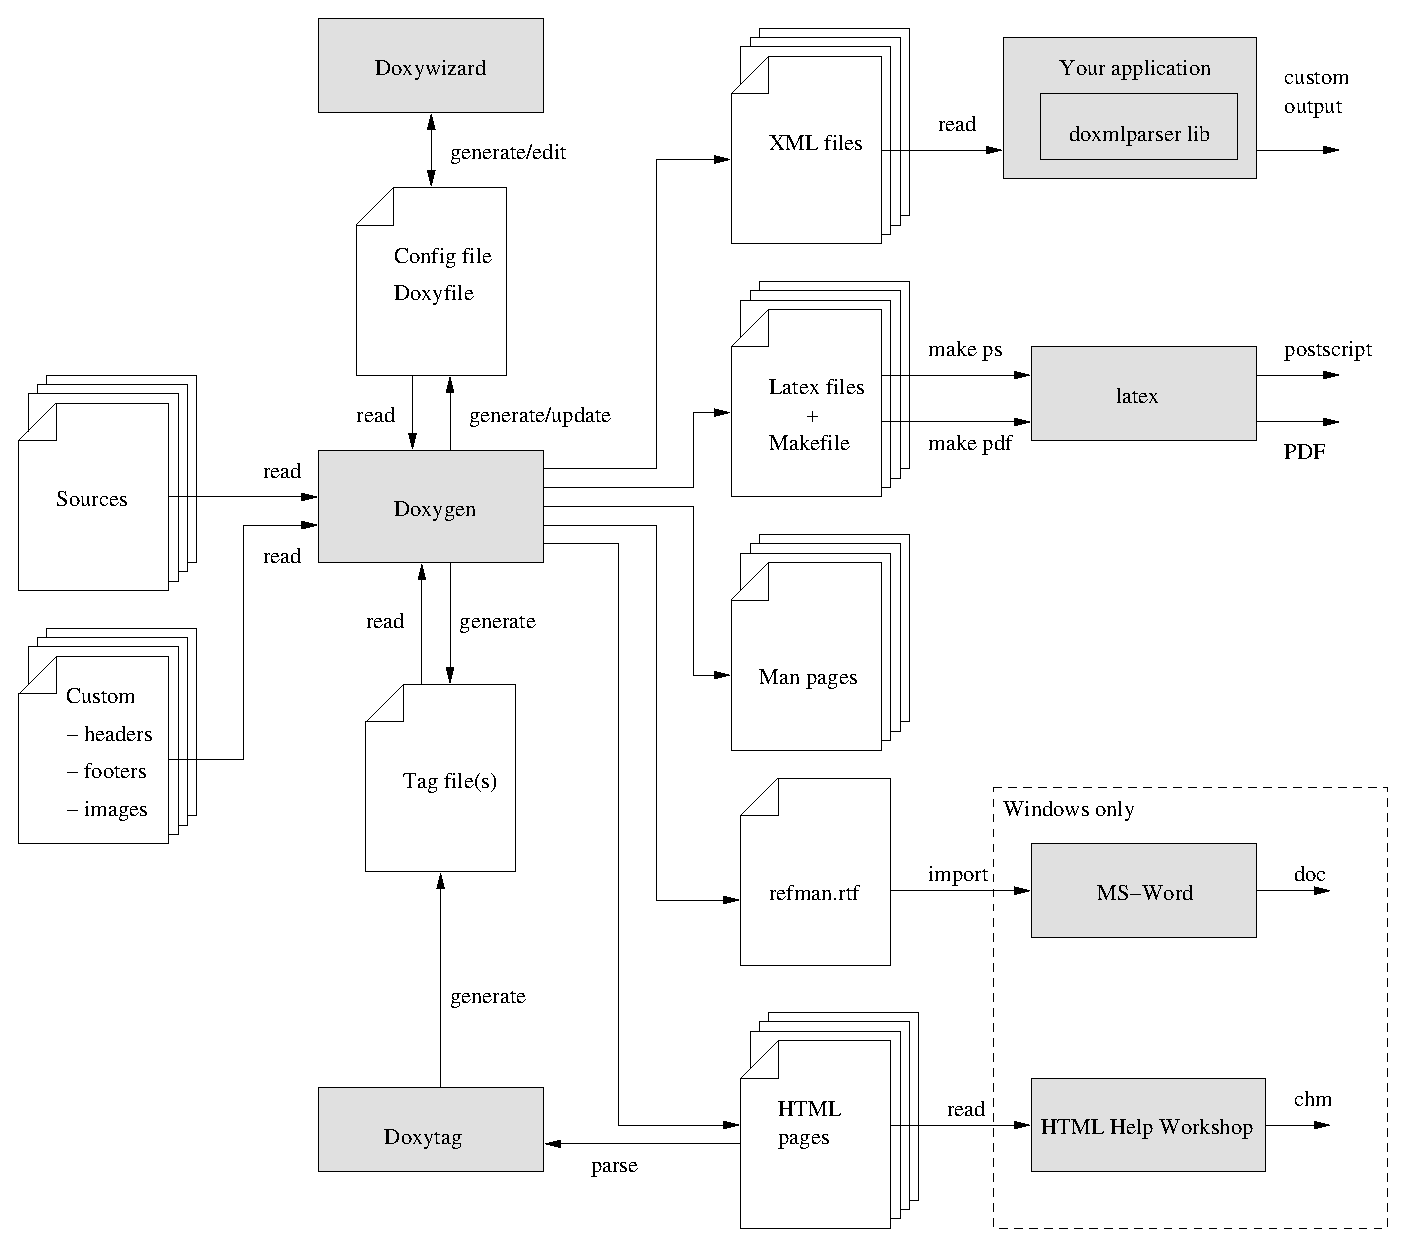
\includegraphics[width=14cm]{infoflow}\caption{Doxygen information flow}
\end{center}
\end{Image}
\hypertarget{starting_step1}{}\section{Step 1: Creating a configuration file}\label{starting_step1}
Doxygen uses a configuration file to determine all of its settings. Each project should get its own configuration file. A project can consist of a single source file, but can also be an entire source tree that is recursively scanned.

To simplify the creation of a configuration file, doxygen can create a template configuration file for you. To do this call {\tt doxygen} from the command line with the {\tt -g} option: 

\footnotesize\begin{verbatim}
doxygen -g <config-file>
\end{verbatim}
\normalsize


where $<$config-file$>$ is the name of the configuration file. If you omit the file name, a file named {\tt Doxyfile} will be created. If a file with the name $<$config-file$>$ already exists, doxygen will rename it to $<$config-file$>$.bak before generating the configuration template. If you use {\tt -} (i.e. the minus sign) as the file name then doxygen will try to read the configuration file from standard input ({\tt stdin}), which can be useful for scripting.

The configuration file has a format that is similar to that of a (simple) Makefile. It consists of a number of assignments (tags) of the form:

{\tt TAGNAME = VALUE} or \par
 {\tt TAGNAME = VALUE1 VALUE2 ... }\par


You can probably leave the values of most tags in a generated template configuration file to their default value. See section \hyperlink{config}{Configuration} for more details about the configuration file.

If you do not wish to edit the config file with a text editor, you should have a look at \hyperlink{doxywizard_usage}{doxywizard}, which is a GUI front-end that can create, read and write doxygen configuration files, and allows setting configuration options by entering them via dialogs.

For a small project consisting of a few C and/or C++ source and header files, you can leave \hyperlink{config_cfg_input}{INPUT} tag empty and doxygen will search for sources in the current directory.

If you have a larger project consisting of a source directory or tree you should assign the root directory or directories to the \hyperlink{config_cfg_input}{INPUT} tag, and add one or more file patterns to the \hyperlink{config_cfg_file_patterns}{FILE\_\-PATTERNS} tag (for instance {\tt $\ast$.cpp $\ast$.h}). Only files that match one of the patterns will be parsed (if the patterns are omitted a list of source extensions is used). For recursive parsing of a source tree you must set the \hyperlink{config_cfg_recursive}{RECURSIVE} tag to {\tt YES}. To further fine-tune the list of files that is parsed the \hyperlink{config_cfg_exclude}{EXCLUDE} and \hyperlink{config_cfg_exclude_patterns}{EXCLUDE\_\-PATTERNS} tags can be used. To omit all {\tt test} directories from a source tree for instance, one could use: 

\footnotesize\begin{verbatim}EXCLUDE_PATTERNS = */test/* 
\end{verbatim}
\normalsize


Doxygen looks at the file's extension to determine how to parse a file. If a file has an {\tt .idl} or {\tt .odl} extension it is treated as an IDL file. If it has a {\tt .java} extension it is treated as a file written in Java. Files ending with {\tt .cs} are treated as C\# files and the {\tt .py} extension selects the Python parser. Finally, files with the extensions {\tt .php}, {\tt .php4}, {\tt .inc} or {\tt .phtml} are treated as PHP sources. Any other extension is parsed as if it is a C/C++ file, where files that end with {\tt .m} are treated as Objective-C source files.

\label{starting_extract_all}
\hypertarget{starting_extract_all}{}
 If you start using doxygen for an existing project (thus without any documentation that doxygen is aware of), you can still get an idea of what the structure is and how the documented result would look like. To do so, you must set the \hyperlink{config_cfg_extract_all}{EXTRACT\_\-ALL} tag in the configuration file to {\tt YES}. Then, doxygen will pretend everything in your sources is documented. Please note that as a consequence warnings about undocumented members will not be generated as long as \hyperlink{config_cfg_extract_all}{EXTRACT\_\-ALL} is set to {\tt YES}.

To analyse an existing piece of software it is useful to cross-reference a (documented) entity with its definition in the source files. Doxygen will generate such cross-references if you set the \hyperlink{config_cfg_source_browser}{SOURCE\_\-BROWSER} tag to {\tt YES}. It can also include the sources directly into the documentation by setting \hyperlink{config_cfg_inline_sources}{INLINE\_\-SOURCES} to {\tt YES} (this can be handy for code reviews for instance).\hypertarget{starting_step2}{}\section{Step 2: Running doxygen}\label{starting_step2}
To generate the documentation you can now enter: 

\footnotesize\begin{verbatim}
doxygen <config-file>
\end{verbatim}
\normalsize


Depending on your settings doxygen will create {\tt html}, {\tt rtf}, {\tt latex}, {\tt xml} and/or {\tt man} directories inside the output directory. As the names suggest these directories contain the generated documentation in HTML, RTF, $\mbox{\LaTeX}$, XML and Unix-Man page format.

The default output directory is the directory in which {\tt doxygen} is started. The root directory to which the output is written can be changed using the \hyperlink{config_cfg_output_directory}{OUTPUT\_\-DIRECTORY}. The format specific directory within the output directory can be selected using the \hyperlink{config_cfg_html_output}{HTML\_\-OUTPUT}, \hyperlink{config_cfg_rtf_output}{RTF\_\-OUTPUT}, \hyperlink{config_cfg_latex_output}{LATEX\_\-OUTPUT}, \hyperlink{config_cfg_xml_output}{XML\_\-OUTPUT}, and \hyperlink{config_cfg_man_output}{MAN\_\-OUTPUT} tags of the configuration file. If the output directory does not exist, {\tt doxygen} will try to create it for you (but it will {\em not\/} try to create a whole path recursively, like {\tt mkdir -p} does).\hypertarget{starting_html_out}{}\subsection{HTML output}\label{starting_html_out}
\index{browser@{browser}} The generated HTML documentation can be viewed by pointing a HTML browser to the {\tt index.html} file in the {\tt html} directory. For the best results a browser that supports cascading style sheets (CSS) should be used (I'm using Mozilla, Safari, Konqueror, and sometimes IE6 to test the generated output).

Some of the features the HTML section (such as \hyperlink{config_cfg_generate_treeview}{GENERATE\_\-TREEVIEW}) require a browser that supports DHTML and Javascript.

If you plan to use the search engine (see \hyperlink{config_cfg_searchengine}{SEARCHENGINE}), you should view the HTML output via a PHP-enabled web server (e.g. apache with the PHP module installed).\hypertarget{starting_latex_out}{}\subsection{LaTeX output}\label{starting_latex_out}
\index{LaTeX@{LaTeX}} The generated $\mbox{\LaTeX}$ documentation must first be compiled by a $\mbox{\LaTeX}$ compiler (I use a recent teTeX distribution). To simplify the process of compiling the generated documentation, {\tt doxygen} writes a {\tt Makefile} into the {\tt latex} directory.

The contents and targets in the {\tt Makefile} depend on the setting of \hyperlink{config_cfg_use_pdflatex}{USE\_\-PDFLATEX}. If it is disabled (set to {\tt NO}), then typing {\tt make} in the {\tt latex} directory a dvi file called {\tt refman.dvi} will be generated. This file can then be viewed using {\tt xdvi} or converted into a PostScript file {\tt refman.ps} by typing {\tt make ps} (this requires {\tt dvips}).

To put 2 pages on one physical page use {\tt make ps\_\-2on1} instead. The resulting PostScript file can be send to a PostScript printer. If you do not have a PostScript printer, you can try to use ghostscript to convert PostScript into something your printer understands.

Conversion to PDF is also possible if you have installed the ghostscript interpreter; just type {\tt make pdf} (or {\tt make pdf\_\-2on1}).

To get the best results for PDF output you should set the \hyperlink{config_cfg_pdf_hyperlinks}{PDF\_\-HYPERLINKS} and \hyperlink{config_cfg_use_pdflatex}{USE\_\-PDFLATEX} tags to {\tt YES}. In this case the {\tt Makefile} will only contain a target to build {\tt refman.pdf} directly.\hypertarget{starting_rtf_out}{}\subsection{RTF output}\label{starting_rtf_out}
\index{RTF@{RTF}} Doxygen combines the RTF output to a single file called refman.rtf. This file is optimized for importing into the Microsoft Word. Certain information is encoded using field. To show the actual value you need to select all (Edit - select all) and then toggle fields (right click and select the option from the drop down menu).\hypertarget{starting_xml_out}{}\subsection{XML output}\label{starting_xml_out}
\index{XML@{XML}} The XML output consists of a structured \char`\"{}dump\char`\"{} of the information gathered by doxygen. Each compound (class/namespace/file/...) has its own XML file and there is also an index file called index.xml.

A file called combine.xslt XSLT script is also generated and can be used to combine all XML files into a single file.

Doxygen also generates two XML schema files index.xsd (for the index file) and compound.xsd (for the compound files). This schema file describes the possible elements, their attributes and how they are structured, i.e. it the describes the grammar of the XML files and can be used for validation or to steer XSLT scripts.

In the addon/doxmlparser directory you can find a parser library for reading the XML output produced by doxygen in an incremental way (see addon/doxmlparser/include/doxmlintf.h for the interface of the library)\hypertarget{starting_man_out}{}\subsection{Man page output}\label{starting_man_out}
The generated man pages can be viewed using the {\tt man} program. You do need to make sure the man directory is in the man path (see the {\tt MANPATH} environment variable). Note that there are some limitations to the capabilities of the man page format, so some information (like class diagrams, cross references and formulas) will be lost.\hypertarget{starting_step3}{}\section{Step 3: Documenting the sources}\label{starting_step3}
Although documenting the sources is presented as step 3, in a new project this should of course be step 1. Here I assume you already have some code and you want doxygen to generate a nice document describing the API and maybe the internals as well.

If the \hyperlink{config_cfg_extract_all}{EXTRACT\_\-ALL} option is set to {\tt NO} in the configuration file (the default), then doxygen will only generate documentation for {\em documented\/} members, files, classes and namespaces. So how do you document these? For members, classes and namespaces there are basically two options: \begin{enumerate}
\item Place a {\em special\/} documentation block in front of the declaration or definition of the member, class or namespace. For file, class and namespace members it is also allowed to place the documention directly after the member. See section \hyperlink{docblocks_specialblock}{Special documentation blocks} to learn more about special documentation blocks. \item Place a special documentation block somewhere else (another file or another location) {\em and\/} put a {\em structural command\/} in the documentation block. A structural command links a documentation block to a certain entity that can be documented (e.g. a member, class, namespace or file). See section \hyperlink{docblocks_structuralcommands}{Documentation at other places} to learn more about structural commands. \end{enumerate}
Files can only be documented using the second option, since there is no way to put a documentation block before a file. Of course, file members (functions, variable, typedefs, defines) do not need an explicit structural command; just putting a special documentation block in front or behind them will do.

The text inside a special documentation block is parsed before it is written to the HTML and/or $\mbox{\LaTeX}$ output files.

\index{parsing@{parsing}} During parsing the following steps take place: \begin{itemize}
\item The special commands inside the documentation are executed. See section \hyperlink{commands}{Special Commands} for an overview of all commands. \item If a line starts with some whitespace followed by one or more asterisks ({\tt $\ast$}) and then optionally more whitespace, then all whitespace and asterisks are removed. \item All resulting blank lines are treated as a paragraph separators. This saves you from placing new-paragraph commands yourself in order to make the generated documentation readable. \item Links are created for words corresponding to documented classes (unless the word is preceded by a \%; then the word will not be linked and the \% sign is removed). \item Links to members are created when certain patterns are found in the text. See section \hyperlink{autolink}{Automatic link generation} for more information on how the automatic link generation works. \item HTML tags that are in the documentation are interpreted and converted to $\mbox{\LaTeX}$ equivalents for the $\mbox{\LaTeX}$ output. See section \hyperlink{htmlcmds}{HTML Commands} for an overview of all supported HTML tags. \end{itemize}


 
\hypertarget{docblocks_specialblock}{}\section{Special documentation blocks}\label{docblocks_specialblock}
A special documentation block is a C or C++ style comment block with some additional markings, so doxygen knows it is a piece of documentation that needs to end up in the generated documentation. For Python and VHDL code there are a different comment conventions, which can be found in section \hyperlink{docblocks_pythonblocks}{Special documentation blocks in Python} and \hyperlink{docblocks_vhdlblocks}{Special documentation blocks in VHDL} respectively.

For each code item there are two (or in some cases three) types of descriptions, which together form the documentation: a {\em brief\/} description and {\em detailed\/} description, both are optional. For methods and functions there is also a third type of description, the so called \char`\"{}in body\char`\"{} description, which consists of the concatenation of all comment blocks found within the body of the method or function.

Having more than one brief or detailed description is allowed (but not recommended, as the order in which the descriptions will appear is not specified).

As the name suggest, a brief description is a short one-liner, whereas the detailed description provides longer, more detailed documentation. An \char`\"{}in body\char`\"{} description can also act as a detailed description or can describe a collection of implementation details. For the HTML output brief descriptions are also use to provide tooltips at places where an item is referenced.

There are several ways to mark a comment block as a detailed description: \begin{enumerate}
\item You can use the JavaDoc style, which consist of a C-style comment block starting with two $\ast$'s, like this:



\footnotesize\begin{verbatim}
/**
 * ... text ...
 */
\end{verbatim}
\normalsize


\item or you can use the Qt style and add an exclamation mark (!) after the opening of a C-style comment block, as shown in this example:



\footnotesize\begin{verbatim}
/*!
 * ... text ...
 */
\end{verbatim}
\normalsize


In both cases the intermediate $\ast$'s are optional, so



\footnotesize\begin{verbatim}
/*!
 ... text ...
*/
\end{verbatim}
\normalsize


is also valid.

\item A third alternative is to use a block of at least two C++ comment lines, where each line starts with an additional slash or an exclamation mark. Here are examples of the two cases:



\footnotesize\begin{verbatim}
///
/// ... text ...
///
\end{verbatim}
\normalsize


or



\footnotesize\begin{verbatim}
//!
//!... text ...
//!
\end{verbatim}
\normalsize


\item 

Some people like to make their comment blocks more visible in the documentation. For this purpose you can use the following:



\footnotesize\begin{verbatim}
/********************************************//**
 *  ... text
 ***********************************************/
\end{verbatim}
\normalsize
 (note the 2 slashes to end the normal comment block and start a special comment block).

or



\footnotesize\begin{verbatim}
/////////////////////////////////////////////////
/// ... text ...
/////////////////////////////////////////////////
\end{verbatim}
\normalsize


\end{enumerate}


For the brief description there are also several posibilities: \begin{enumerate}
\item One could use the \hyperlink{commands_cmdbrief}{$\backslash$brief} command with one of the above comment blocks. This command ends at the end of a paragraph, so the detailed description follows after an empty line.

Here is an example:



\footnotesize\begin{verbatim}
/*! \brief Brief description.
 *         Brief description continued.
 *
 *  Detailed description starts here.
 */
\end{verbatim}
\normalsize


\item If \hyperlink{config_cfg_javadoc_autobrief}{JAVADOC\_\-AUTOBRIEF} is set to {\tt YES} in the configuration file, then using JavaDoc style comment blocks will automatically start a brief description which ends at the first dot followed by a space or new line. Here is an example:



\footnotesize\begin{verbatim}
/** Brief description which ends at this dot. Details follow
 *  here.
 */
\end{verbatim}
\normalsize
 The option has the same effect for multi-line special C++ comments: 

\footnotesize\begin{verbatim}
/// Brief description which ends at this dot. Details follow
/// here.
\end{verbatim}
\normalsize


\item A third option is to use a special C++ style comment which does not span more than one line. Here are two examples: 

\footnotesize\begin{verbatim}
/// Brief description.
/** Detailed description. */
\end{verbatim}
\normalsize


or



\footnotesize\begin{verbatim}
//! Brief descripion.

//! Detailed description 
//! starts here.
\end{verbatim}
\normalsize


Note the blank line in the last example, which is required to separate the brief description from the block containing the detailed description. The \hyperlink{config_cfg_javadoc_autobrief}{JAVADOC\_\-AUTOBRIEF} should also be set to {\tt NO} for this case.

\end{enumerate}


As you can see doxygen is quite flexible. The following however is not legal



\footnotesize\begin{verbatim}
//! Brief description, which is
//! really a detailed description since it spans multiple lines.
/*! Oops, another detailed description!
 */
\end{verbatim}
\normalsize


because doxygen only allows one brief and one detailed description.

Furthermore, if there is one brief description before a declaration and one before a definition of a code item, only the one before the {\em declaration\/} will be used. If the same situation occurs for a detailed description, the one before the {\em definition\/} is preferred and the one before the declaration will be ignored.

Here is an example of a documented piece of C++ code using the Qt style: 

\begin{DocInclude}\begin{verbatim}//!  A test class. 
/*!
  A more elaborate class description.
*/

class Test
{
  public:

    //! An enum.
    /*! More detailed enum description. */
    enum TEnum { 
                 TVal1, /*!< Enum value TVal1. */  
                 TVal2, /*!< Enum value TVal2. */  
                 TVal3  /*!< Enum value TVal3. */  
               } 
         //! Enum pointer.
         /*! Details. */
         *enumPtr, 
         //! Enum variable.
         /*! Details. */
         enumVar;  
    
    //! A constructor.
    /*!
      A more elaborate description of the constructor.
    */
    Test();

    //! A destructor.
    /*!
      A more elaborate description of the destructor.
    */
   ~Test();
    
    //! A normal member taking two arguments and returning an integer value.
    /*!
      \param a an integer argument.
      \param s a constant character pointer.
      \return The test results
      \sa Test(), ~Test(), testMeToo() and publicVar()
    */
    int testMe(int a,const char *s);
       
    //! A pure virtual member.
    /*!
      \sa testMe()
      \param c1 the first argument.
      \param c2 the second argument.
    */
    virtual void testMeToo(char c1,char c2) = 0;
   
    //! A public variable.
    /*!
      Details.
    */
    int publicVar;
       
    //! A function variable.
    /*!
      Details.
    */
    int (*handler)(int a,int b);
};

\end{verbatim}
\end{DocInclude}
 

The one-line comments contain a brief description, whereas the multi-line comment blocks contain a more detailed description.

The brief descriptions are included in the member overview of a class, namespace or file and are printed using a small italic font (this description can be hidden by setting \hyperlink{config_cfg_brief_member_desc}{BRIEF\_\-MEMBER\_\-DESC} to {\tt NO} in the config file). By default the brief descriptions become the first sentence of the detailed descriptions (but this can be changed by setting the \hyperlink{config_cfg_repeat_brief}{REPEAT\_\-BRIEF} tag to {\tt NO}). Both the brief and the detailed descriptions are optional for the Qt style.

By default a JavaDoc style documentation block behaves the same way as a Qt style documentation block. This is not according the JavaDoc specification however, where the first sentence of the documentation block is automatically treated as a brief description. To enable this behaviour you should set \hyperlink{config_cfg_javadoc_autobrief}{JAVADOC\_\-AUTOBRIEF} to YES in the configuration file. If you enable this option and want to put a dot in the middle of a sentence without ending it, you should put a backslash and a space after it. Here is an example: 

\footnotesize\begin{verbatim}
  /** Brief description (e.g.\ using only a few words). Details follow. */
\end{verbatim}
\normalsize


Here is the same piece of code as shown above, this time documented using the JavaDoc style and \hyperlink{config_cfg_javadoc_autobrief}{JAVADOC\_\-AUTOBRIEF} set to YES: 

\begin{DocInclude}\begin{verbatim}/**
 *  A test class. A more elaborate class description.
 */

class Test
{
  public:

    /** 
     * An enum.
     * More detailed enum description.
     */

    enum TEnum { 
          TVal1, /**< enum value TVal1. */  
          TVal2, /**< enum value TVal2. */  
          TVal3  /**< enum value TVal3. */  
         } 
       *enumPtr, /**< enum pointer. Details. */
       enumVar;  /**< enum variable. Details. */
       
      /**
       * A constructor.
       * A more elaborate description of the constructor.
       */
      Test();

      /**
       * A destructor.
       * A more elaborate description of the destructor.
       */
     ~Test();
    
      /**
       * a normal member taking two arguments and returning an integer value.
       * @param a an integer argument.
       * @param s a constant character pointer.
       * @see Test()
       * @see ~Test()
       * @see testMeToo()
       * @see publicVar()
       * @return The test results
       */
       int testMe(int a,const char *s);
       
      /**
       * A pure virtual member.
       * @see testMe()
       * @param c1 the first argument.
       * @param c2 the second argument.
       */
       virtual void testMeToo(char c1,char c2) = 0;
   
      /** 
       * a public variable.
       * Details.
       */
       int publicVar;
       
      /**
       * a function variable.
       * Details.
       */
       int (*handler)(int a,int b);
};

\end{verbatim}
\end{DocInclude}
 

Similarly, if one wishes the first sentence of a Qt style documentation block to automatically be treated as a brief description, one may set \hyperlink{config_cfg_qt_autobrief}{QT\_\-AUTOBRIEF} to YES in the configuration file.

Unlike most other documentation systems, doxygen also allows you to put the documentation of members (including global functions) in front of the {\em definition\/}. This way the documentation can be placed in the source file instead of the header file. This keeps the header file compact, and allows the implementer of the members more direct access to the documentation. As a compromise the brief description could be placed before the declaration and the detailed description before the member definition.\hypertarget{docblocks_memberdoc}{}\section{Putting documentation after members}\label{docblocks_memberdoc}
If you want to document the members of a file, struct, union, class, or enum, and you want to put the documentation for these members inside the compound, it is sometimes desired to place the documentation block after the member instead of before. For this purpose you have to put an additional $<$ marker in the comment block. Note that this also works for the parameters of a function.

Here are some examples: 

\footnotesize\begin{verbatim}
int var; /*!< Detailed description after the member */
\end{verbatim}
\normalsize
 This block can be used to put a Qt style detailed documentation block {\em after\/} a member. Other ways to do the same are: 

\footnotesize\begin{verbatim}
int var; /**< Detailed description after the member */
\end{verbatim}
\normalsize
 or 

\footnotesize\begin{verbatim}
int var; //!< Detailed description after the member
         //!< 
\end{verbatim}
\normalsize
 or 

\footnotesize\begin{verbatim}
int var; ///< Detailed description after the member
         ///< 
\end{verbatim}
\normalsize


Most often one only wants to put a brief description after a member. This is done as follows: 

\footnotesize\begin{verbatim}
int var; //!< Brief description after the member
\end{verbatim}
\normalsize
 or 

\footnotesize\begin{verbatim}
int var; ///< Brief description after the member
\end{verbatim}
\normalsize


Note that these blocks have the same structure and meaning as the special comment blocks in the previous section only the $<$ indicates that the member is located in front of the block instead of after the block.

Here is an example of the use of these comment blocks: 

\begin{DocInclude}\begin{verbatim}/*! A test class */

class Test
{
  public:
    /** An enum type. 
     *  The documentation block cannot be put after the enum! 
     */
    enum EnumType
    {
      int EVal1,     /**< enum value 1 */
      int EVal2      /**< enum value 2 */
    };
    void member();   //!< a member function.
    
  protected:
    int value;       /*!< an integer value */
};
\end{verbatim}
\end{DocInclude}
 

\begin{Desc}
\item[Warning:]These blocks can only be used to document {\em members\/} and {\em parameters\/}. They cannot be used to document files, classes, unions, structs, groups, namespaces and enums themselves. Furthermore, the structural commands mentioned in the next section (like {\tt $\backslash$class}) are ignored inside these comment blocks.\end{Desc}
\hypertarget{docblocks_structuralcommands}{}\section{Documentation at other places}\label{docblocks_structuralcommands}
So far we have assumed that the documentation blocks are always located {\em in\/} {\em front\/} of the declaration or definition of a file, class or namespace or in front or after one of its members. Although this is often comfortable, there may sometimes be reasons to put the documentation somewhere else. For documenting a file this is even required since there is no such thing as \char`\"{}in front of a file\char`\"{}.

Doxygen allows you to put your documentation blocks practically anywhere (the exception is inside the body of a function or inside a normal C style comment block).

The price you pay for not putting the documentation block directly before (or after) an item is the need to put a structural command inside the documentation block, which leads to some duplication of information. So in practice you should {\em avoid\/} the use of structural commands {\em unless\/} other requirements force you to do so.

Structural commands (like all other commands) start with a backslash ({\tt $\backslash$}), or an at-sign ({\tt @}) if you prefer JavaDoc style, followed by a command name and one or more parameters. For instance, if you want to document the class {\tt Test} in the example above, you could have also put the following documentation block somewhere in the input that is read by doxygen: 

\footnotesize\begin{verbatim}
/*! \class Test
    \brief A test class.

    A more detailed class description.
*/
\end{verbatim}
\normalsize


Here the special command {\tt $\backslash$class} is used to indicate that the comment block contains documentation for the class {\tt Test}. Other structural commands are: \begin{itemize}
\item {\tt $\backslash$struct} to document a C-struct. \item {\tt $\backslash$union} to document a union. \item {\tt $\backslash$enum} to document an enumeration type. \item {\tt $\backslash$fn} to document a function. \item {\tt $\backslash$var} to document a variable or typedef or enum value. \item {\tt $\backslash$def} to document a \#define. \item {\tt $\backslash$typedef} to document a type definition. \item {\tt $\backslash$file} to document a file. \item {\tt $\backslash$namespace} to document a namespace. \item {\tt $\backslash$package} to document a Java package. \item {\tt $\backslash$interface} to document an IDL interface. \end{itemize}
See section \hyperlink{commands}{Special Commands} for detailed information about these and many other commands.

To document a member of a C++ class, you must also document the class itself. The same holds for namespaces. To document a global C function, typedef, enum or preprocessor definition you must first document the file that contains it (usually this will be a header file, because that file contains the information that is exported to other source files).

Let's repeat that, because it is often overlooked: to document global objects (functions, typedefs, enum, macros, etc), you {\em must\/} document the file in which they are defined. In other words, there {\em must\/} at least be a 

\footnotesize\begin{verbatim}/*! \file */ \end{verbatim}
\normalsize
 or a 

\footnotesize\begin{verbatim}/** @file */ \end{verbatim}
\normalsize
 line in this file.

Here is an example of a C header named {\tt structcmd.h} that is documented using structural commands: 

\begin{DocInclude}\begin{verbatim}/*! \file structcmd.h
    \brief A Documented file.
    
    Details.
*/

/*! \def MAX(a,b)
    \brief A macro that returns the maximum of \a a and \a b.
   
    Details.
*/

/*! \var typedef unsigned int UINT32
    \brief A type definition for a .
    
    Details.
*/

/*! \var int errno
    \brief Contains the last error code.

    \warning Not thread safe!
*/

/*! \fn int open(const char *pathname,int flags)
    \brief Opens a file descriptor.

    \param pathname The name of the descriptor.
    \param flags Opening flags.
*/

/*! \fn int close(int fd)
    \brief Closes the file descriptor \a fd.
    \param fd The descriptor to close.
*/

/*! \fn size_t write(int fd,const char *buf, size_t count)
    \brief Writes \a count bytes from \a buf to the filedescriptor \a fd.
    \param fd The descriptor to write to.
    \param buf The data buffer to write.
    \param count The number of bytes to write.
*/

/*! \fn int read(int fd,char *buf,size_t count)
    \brief Read bytes from a file descriptor.
    \param fd The descriptor to read from.
    \param buf The buffer to read into.
    \param count The number of bytes to read.
*/

#define MAX(a,b) (((a)>(b))?(a):(b))
typedef unsigned int UINT32;
int errno;
int open(const char *,int);
int close(int);
size_t write(int,const char *, size_t);
int read(int,char *,size_t);
\end{verbatim}
\end{DocInclude}
 

Because each comment block in the example above contains a structural command, all the comment blocks could be moved to another location or input file (the source file for instance), without affecting the generated documentation. The disadvantage of this approach is that prototypes are duplicated, so all changes have to be made twice! Because of this you should first consider if this is really needed, and avoid structural commands if possible. I often receive examples that contain $\backslash$fn command in comment blocks which are place in front of a function. This is clearly a case where the $\backslash$fn command is redundant and will only lead to problems.\hypertarget{docblocks_pythonblocks}{}\section{Special documentation blocks in Python}\label{docblocks_pythonblocks}
For Python there is a standard way of documenting the code using so called documentation strings. Such strings are stored in {\tt \_\-\_\-doc\_\-\_\-} and can be retrieved at runtime. Doxygen will extract such comments and assume they have to be represented in a preformatted way.



\begin{DocInclude}\begin{verbatim}"""@package docstring
Documentation for this module.

More details.
"""

def func():
    """Documentation for a function.

    More details.
    """
    pass

class PyClass:
    """Documentation for a class.

    More details.
    """
   
    def __init__(self):
        """The constructor."""
        self._memVar = 0;
   
    def PyMethod(self):
        """Documentation for a method."""
        pass
     
\end{verbatim}
\end{DocInclude}
 

Note that in this case none of doxygen's \hyperlink{commands_cmd_intro}{special commands} are supported.

There is also another way to document Python code using comments that start with \char`\"{}\#\#\char`\"{}. These type of comment blocks are more in line with the way documentation blocks work for the other languages supported by doxygen and this also allows the use of special commands.

Here is the same example again but now using doxygen style comments:



\begin{DocInclude}\begin{verbatim}## @package pyexample
#  Documentation for this module.
#
#  More details.

## Documentation for a function.
#
#  More details.
def func():
    pass

## Documentation for a class.
#
#  More details.
class PyClass:
   
    ## The constructor.
    def __init__(self):
        self._memVar = 0;
   
    ## Documentation for a method.
    #  @param self The object pointer.
    def PyMethod(self):
        pass
     
    ## A class variable.
    classVar = 0;

    ## @var _memVar
    #  a member variable
\end{verbatim}
\end{DocInclude}
 

Since python looks more like Java than like C or C++, you should set \hyperlink{config_cfg_optimize_output_java}{OPTMIZE\_\-OUTPUT\_\-JAVA} to {\tt YES} in the config file.

\hypertarget{docblocks_vhdlblocks}{}\section{Special documentation blocks in VHDL}\label{docblocks_vhdlblocks}
For VHDL a comment normally start with \char`\"{}--\char`\"{}. Doxygen will extract comments starting with \char`\"{}--!\char`\"{}. There are only two types of comment blocks in VHDL; a one line --! comment representing a brief description, and a multiline --! comment (where the --! prefix is repeated for each line) representing a detailed description.

Comments are always located in front of the item that is being documented with one exception: for ports the comment can also be after the item and is then treated as a brief description for the port.

Here is an example VHDL file with doxygen comments:



\begin{DocInclude}\begin{verbatim}-------------------------------------------------------
--! @file
--! @brief 2:1 Mux using with-select
-------------------------------------------------------

--! Use standard library
library ieee;
--! Use logic elements
    use ieee.std_logic_1164.all;

--! Mux entity brief description

--! Detailed description of this 
--! mux design element.
entity mux_using_with is
    port (
        din_0   : in  std_logic; --! Mux first input
        din_1   : in  std_logic; --! Mux Second input
        sel     : in  std_logic; --! Select input
        mux_out : out std_logic  --! Mux output
    );
end entity;

--! @brief Architure definition of the MUX
--! @details More details about this mux element.
architecture behavior of mux_using_with is
begin
    with (sel) select
    mux_out <= din_0 when '0',
               din_1 when others;
end architecture;

\end{verbatim}
\end{DocInclude}
 

To get proper looking output you need to set \hyperlink{config_cfg_optimize_output_vhdl}{OPTIMIZE\_\-OUTPUT\_\-VHDL} to {\tt YES} in the config file. This will also affect a number of other settings. When they were not already set correctly doxygen will produce a warning telling which settings where overruled. 
Doxygen provides a number of ways to create lists of items.

{\bf Using dashes}

By putting a number of column-aligned minus signs at the start of a line, a bullet list will automatically be generated. Numbered lists can also be generated by using a minus followed by a hash. Nesting of lists is allowed and is based on indentation of the items.

Here is an example: 

\footnotesize\begin{verbatim}
  /*! 
   *  A list of events:
   *    - mouse events
   *         -# mouse move event
   *         -# mouse click event\n
   *            More info about the click event.
   *         -# mouse double click event
   *    - keyboard events
   *         -# key down event
   *         -# key up event
   *
   *  More text here.
   */
\end{verbatim}
\normalsize
 The result will be:

A list of events:\begin{itemize}
\item mouse events\begin{enumerate}
\item mouse move event\item mouse click event\par
 More info about the click event.\item mouse double click event\end{enumerate}
\item keyboard events\begin{enumerate}
\item key down event\item key up event\end{enumerate}
\end{itemize}


More text here.

If you use tabs for indentation within lists, please make sure that \hyperlink{config_cfg_tab_size}{TAB\_\-SIZE} in the configuration file is set to the correct tab size.

You can end a list by starting a new paragraph or by putting a dot (.) on an empty line at the same indent level as the list you would like to end.

Here is an example that speaks for itself:



\footnotesize\begin{verbatim}
/**
 * Text before the list
 * - list item 1
 *   - sub item 1
 *     - sub sub item 1
 *     - sub sub item 2
 *     . 
 *     The dot above ends the sub sub item list.
 *     More text for the first sub item
 *   .
 *   The dot above ends the first sub item.
 *   More text for the first list item
 *   - sub item 2
 *   - sub item 3
 * - list item 2
 * .
 * More text in the same paragraph.
 *
 * More text in a new paragraph.
 */
\end{verbatim}
\normalsize


{\bf Using HTML commands}

If you like you can also use HTML commands inside the documentation blocks. Using these commands has the advantage that it is more natural for list items that consist of multiple paragraphs.

Here is the above example with HTML commands: 

\footnotesize\begin{verbatim}
  /*! 
   *  A list of events:
   *  <ul>
   *  <li> mouse events
   *     <ol>
   *     <li>mouse move event
   *     <li>mouse click event\n
   *         More info about the click event.
   *     <li>mouse double click event
   *     </ol>
   *  <li> keyboard events
   *     <ol>     
   *     <li>key down event
   *     <li>key up event
   *     </ol>
   *  </ul>
   *  More text here.
   */
\end{verbatim}
\normalsize


\begin{Desc}
\item[Note:]In this case the indentation is not important.\end{Desc}
{\bf Using $\backslash$arg or @li}

For compatibility with the Troll Tech's internal documentation tool and with KDoc, doxygen has two commands that can be used to create simple unnested lists.

See \hyperlink{commands_cmdarg}{$\backslash$arg} and \hyperlink{commands_cmdli}{$\backslash$li} for more info.

 
Doxygen has three mechanisms to group things together. One mechanism works at a global level, creating a new page for each group. These groups are called \hyperlink{grouping_modules}{'modules'} in the documentation. The second mechanism works within a member list of some compound entity, and is refered to as a \hyperlink{grouping_memgroup}{'member groups'}. For \hyperlink{commands_cmdpage}{pages} there is a third grouping mechanism referred to as \hyperlink{grouping_subpaging}{subpaging}.\hypertarget{grouping_modules}{}\section{Modules}\label{grouping_modules}
Modules are a way to group things together on a separate page. You can document a group as a whole, as well as all individual members. Members of a group can be files, namespaces, classes, functions, variables, enums, typedefs, and defines, but also other groups.

To define a group, you should put the \hyperlink{commands_cmddefgroup}{$\backslash$defgroup} command in a special comment block. The first argument of the command is a label that should uniquely identify the group. The second argument is the name or title of the group as it should appear in the documentation.

You can make an entity a member of a specific group by putting a \hyperlink{commands_cmdingroup}{$\backslash$ingroup} command inside its documentation block.

To avoid putting \hyperlink{commands_cmdingroup}{$\backslash$ingroup} commands in the documentation for each member you can also group members together by the open marker {\tt @\{} before the group and the closing marker {\tt @\}} after the group. The markers can be put in the documentation of the group definition or in a separate documentation block.

Groups themselves can also be nested using these grouping markers.

You will get an error message when you use the same group label more than once. If you don't want doxygen to enforce unique labels, then you can use \hyperlink{commands_cmdaddtogroup}{$\backslash$addtogroup} instead of \hyperlink{commands_cmddefgroup}{$\backslash$defgroup}. It can be used exactly like \hyperlink{commands_cmddefgroup}{$\backslash$defgroup}, but when the group has been defined already, then it silently merges the existing documentation with the new one. The title of the group is optional for this command, so you can use 

\footnotesize\begin{verbatim}
/** \addtogroup <label> */
/*\@{*/
/*\@}*/
\end{verbatim}
\normalsize
 to add additional members to a group that is defined in more detail elsewhere.

Note that compound entities (like classes, files and namespaces) can be put into multiple groups, but members (like variable, functions, typedefs and enums) can only be a member of one group (this restriction is in place to avoid ambiguous linking targets in case a member is not documented in the context of its class, namespace or file, but only visible as part of a group).

Doxygen will put members into the group whose definition has the highest \char`\"{}priority\char`\"{}: e.g. An explicit \hyperlink{commands_cmdingroup}{$\backslash$ingroup} overrides an implicit grouping definition via {\tt @\{} {\tt @\}}. Conflicting grouping definitions with the same priority trigger a warning, unless one definition was for a member without any explicit documentation.

The following example puts VarInA into group A and silently resolves the conflict for IntegerVariable by putting it into group IntVariables, because the second instance of IntegerVariable is undocumented:



\footnotesize\begin{verbatim}

/**
 * \ingroup A
 */
extern int VarInA;

/**
 * \defgroup IntVariables Global integer variables
 */
/*@{*/

/** an integer variable */
extern int IntegerVariable;

/*@}*/

....

/**
 * \defgroup Variables Global variables
 */
/*@{*/

/** a variable in group A */
int VarInA;

int IntegerVariable;

/*@}*/
\end{verbatim}
\normalsize


The \hyperlink{commands_cmdref}{$\backslash$ref} command can be used to refer to a group. The first argument of the $\backslash$ref command should be group's label. To use a custom link name, you can put the name of the links in double quotes after the label, as shown by the following example 

\footnotesize\begin{verbatim}
This is the \ref group_label "link" to this group.
\end{verbatim}
\normalsize


The priorities of grouping definitions are (from highest to lowest): \hyperlink{commands_cmdingroup}{$\backslash$ingroup}, \hyperlink{commands_cmddefgroup}{$\backslash$defgroup}, \hyperlink{commands_cmdaddtogroup}{$\backslash$addtogroup}, \hyperlink{commands_cmdweakgroup}{$\backslash$weakgroup}. The last command is exactly like \hyperlink{commands_cmdaddtogroup}{$\backslash$addtogroup} with a lower priority. It was added to allow \char`\"{}lazy\char`\"{} grouping definitions: you can use commands with a higher priority in your .h files to define the hierarchy and \hyperlink{commands_cmdweakgroup}{$\backslash$weakgroup} in .c files without having to duplicate the hierarchy exactly.

\begin{Desc}
\item[Example:]

\begin{VerbInclude}\begin{verbatim}/** @defgroup group1 The First Group
 *  This is the first group
 *  @{
 */

/** @brief class C1 in group 1 */
class C1 {};

/** @brief class C2 in group 1 */
class C2 {};

/** function in group 1 */
void func() {}

/** @} */ // end of group1

/**
 *  @defgroup group2 The Second Group
 *  This is the second group
 */

/** @defgroup group3 The Third Group
 *  This is the third group
 */

/** @defgroup group4 The Fourth Group
 *  @ingroup group3
 *  Group 4 is a subgroup of group 3
 */

/**
 *  @ingroup group2
 *  @brief class C3 in group 2
 */
class C3 {};

/** @ingroup group2
 *  @brief class C4 in group 2
 */
class C4 {};

/** @ingroup group3
 *  @brief class C5 in @link group3 the third group@endlink.
 */
class C5 {};

/** @ingroup group1 group2 group3 group4
 *  namespace N1 is in four groups
 *  @sa @link group1 The first group@endlink, group2, group3, group4 
 *
 *  Also see @ref mypage2
 */
namespace N1 {};

/** @file
 *  @ingroup group3
 *  @brief this file in group 3
 */

/** @defgroup group5 The Fifth Group
 *  This is the fifth group
 *  @{
 */

/** @page mypage1 This is a section in group 5
 *  Text of the first section
 */

/** @page mypage2 This is another section in group 5
 *  Text of the second section
 */

/** @} */ // end of group5

/** @addtogroup group1
 *  
 *  More documentation for the first group.
 *  @{
 */

/** another function in group 1 */
void func2() {}

/** yet another function in group 1 */
void func3() {}

/** @} */ // end of group1

\end{verbatim}
\end{VerbInclude}
\end{Desc}
\hypertarget{grouping_memgroup}{}\section{Member Groups}\label{grouping_memgroup}
If a compound (e.g. a class or file) has many members, it is often desired to group them together. Doxygen already automatically groups things together on type and protection level, but maybe you feel that this is not enough or that that default grouping is wrong. For instance, because you feel that members of different (syntactic) types belong to the same (semantic) group.

A member group is defined by a 

\footnotesize\begin{verbatim}
//@{ 
  ...
//@}
\end{verbatim}
\normalsize
 block or a 

\footnotesize\begin{verbatim}
/*@{*/ 
  ... 
/*@}*/ 
\end{verbatim}
\normalsize
 block if you prefer C style comments. Note that the members of the group should be physcially inside the member group's body.

Before the opening marker of a block a separate comment block may be placed. This block should contain the \hyperlink{commands_cmdname}{@name} (or \hyperlink{commands_cmdname}{$\backslash$name}) command and is used to specify the header of the group. Optionally, the comment block may also contain more detailed information about the group.

Nesting of member groups is not allowed.

If all members of a member group inside a class have the same type and protection level (for instance all are static public members), then the whole member group is displayed as a subgroup of the type/protection level group (the group is displayed as a subsection of the \char`\"{}Static Public Members\char`\"{} section for instance). If two or more members have different types, then the group is put at the same level as the automatically generated groups. If you want to force all member-groups of a class to be at the top level, you should put a \hyperlink{commands_cmdnosubgrouping}{$\backslash$nosubgrouping} command inside the documentation of the class.

\begin{Desc}
\item[Example:]

\begin{VerbInclude}\begin{verbatim}/** A class. Details */
class Test
{
  public:
    //@{
    /** Same documentation for both members. Details */
    void func1InGroup1();
    void func2InGroup1();
    //@}

    /** Function without group. Details. */
    void ungroupedFunction();
    void func1InGroup2();
  protected:
    void func2InGroup2();
};

void Test::func1InGroup1() {}
void Test::func2InGroup1() {}

/** @name Group2
 *  Description of group 2. 
 */
//@{
/** Function 2 in group 2. Details. */
void Test::func2InGroup2() {}
/** Function 1 in group 2. Details. */
void Test::func1InGroup2() {}
//@}

/*! \file 
 *  docs for this file
 */

//@{
//! one description for all members of this group 
//! (because DISTRIBUTE_GROUP_DOC is YES in the config file)
#define A 1
#define B 2
void glob_func();
//@}
\end{verbatim}
\end{VerbInclude}
\end{Desc}


Here Group1 is displayed as a subsection of the \char`\"{}Public Members\char`\"{}. And Group2 is a separate section because it contains members with different protection levels (i.e. public and protected).

\hypertarget{grouping_subpaging}{}\section{Subpaging}\label{grouping_subpaging}
Information can be grouped into pages using the \hyperlink{commands_cmdpage}{$\backslash$page} and \hyperlink{commands_cmdsubpage}{$\backslash$mainpage} commands. Normally, this results in a flat list of pages, where the \char`\"{}main\char`\"{} page is the first in the list.

Instead of adding structure using the approach decribed in section \hyperlink{grouping_modules}{modules} it is often more natural and convienent to add additional structure to the pages using the \hyperlink{commands_cmdsubpage}{$\backslash$subpage} command.

For a page A the $\backslash$subpage command adds a link to another page B and at the same time makes page B a subpage of A. This has the effect of making two groups GA and GB, where GB is part of GA, page A is put in group GA, and page B is put in group GB.

 
Doxygen allows you to put $\mbox{\LaTeX}$ formulas in the output (this works only for the HTML and $\mbox{\LaTeX}$ output, not for the RTF nor for the man page output). To be able to include formulas (as images) in the HTML documentation, you will also need to have the following tools installed \begin{itemize}
\item {\tt latex:} the $\mbox{\LaTeX}$ compiler, needed to parse the formulas. To test I have used the teTeX 1.0 distribution. \item {\tt dvips:} a tool to convert DVI files to PostScript files I have used version 5.92b from Radical Eye software for testing. \item {\tt gs:} the GhostScript interpreter for converting PostScript files to bitmaps. I have used Aladdin GhostScript 8.0 for testing. \end{itemize}


There are three ways to include formulas in the documentation. \begin{enumerate}
\item Using in-text formulas that appear in the running text. These formulas should be put between a pair of $\backslash$f\$ commands, so 

\footnotesize\begin{verbatim}
  The distance between \f$(x_1,y_1)\f$ and \f$(x_2,y_2)\f$ is 
  \f$\sqrt{(x_2-x_1)^2+(y_2-y_1)^2}\f$.
\end{verbatim}
\normalsize
 results in:

The distance between $(x_1,y_1)$ and $(x_2,y_2)$ is $\sqrt{(x_2-x_1)^2+(y_2-y_1)^2}$. \par
 \item Unnumbered displayed formulas that are centered on a separate line. These formulas should be put between $\backslash$f\mbox{[} and $\backslash$f\mbox{]} commands. An example: 

\footnotesize\begin{verbatim}
  \f[
    |I_2|=\left| \int_{0}^T \psi(t) 
             \left\{ 
                u(a,t)-
                \int_{\gamma(t)}^a 
                \frac{d\theta}{k(\theta,t)}
                \int_{a}^\theta c(\xi)u_t(\xi,t)\,d\xi
             \right\} dt
          \right|
  \f]
\end{verbatim}
\normalsize
 results in: \[ |I_2|=\left| \int_{0}^T \psi(t) \left\{ u(a,t)- \int_{\gamma(t)}^a \frac{d\theta}{k(\theta,t)} \int_{a}^\theta c(\xi)u_t(\xi,t)\,d\xi \right\} dt \right| \] \item Formulas or other latex elements that are not in a math environment can be specified using $\backslash$f\{environment\}, where {\tt environment} is the name of the $\mbox{\LaTeX}$ environment, the corresponding end command is $\backslash$f\}. Here is an example for an equation array 

\footnotesize\begin{verbatim}
   \f{eqnarray*}{
        g &=& \frac{Gm_2}{r^2} \\ 
          &=& \frac{(6.673 \times 10^{-11}\,\mbox{m}^3\,\mbox{kg}^{-1}\,
              \mbox{s}^{-2})(5.9736 \times 10^{24}\,\mbox{kg})}{(6371.01\,\mbox{km})^2} \\ 
          &=& 9.82066032\,\mbox{m/s}^2
   \f}
\end{verbatim}
\normalsize
 which results in: \begin{eqnarray*} g &=& \frac{Gm_2}{r^2} \\ &=& \frac{(6.673 \times 10^{-11}\,\mbox{m}^3\,\mbox{kg}^{-1}\, \mbox{s}^{-2})(5.9736 \times 10^{24}\,\mbox{kg})}{(6371.01\,\mbox{km})^2} \\ &=& 9.82066032\,\mbox{m/s}^2 \end{eqnarray*} \end{enumerate}
For the first two commands one should make sure formulas contain valid commands in $\mbox{\LaTeX}$'s math-mode. For the third command the section should contain valid command for the specific environment.

\begin{Desc}
\item[Warning:]Currently, doxygen is not very fault tolerant in recovering from typos in formulas. It may be necessary to remove the file {\tt formula.repository} that is written to the html directory to get rid of an incorrect formula.\end{Desc}
 
Doxygen has built-in support to generate inheritance diagrams for C++ classes.

Doxygen can use the \char`\"{}dot\char`\"{} tool from graphviz 1.5 to generate more advanced diagrams and graphs. Graphviz is an \char`\"{}open-sourced\char`\"{}, cross-platform graph drawing toolkit and can be found at \href{http://www.graphviz.org/}{\tt http://www.graphviz.org/}

If you have the \char`\"{}dot\char`\"{} tool available in the path, you can set \hyperlink{config_cfg_have_dot}{HAVE\_\-DOT} to {\tt YES} in the configuration file to let doxygen use it.

Doxygen uses the \char`\"{}dot\char`\"{} tool to generate the following graphs: \begin{itemize}
\item if \hyperlink{config_cfg_graphical_hierarchy}{GRAPHICAL\_\-HIERARCHY} is set to {\tt YES}, a graphical representation of the class hierarchy will be drawn, along with the textual one. Currently this feature is supported for HTML only.\par
 {\bf Warning:} When you have a very large class hierarchy where many classes derive from a common base class, the resulting image may become too big to handle for some browsers. \item if \hyperlink{config_cfg_class_graph}{CLASS\_\-GRAPH} is set to {\tt YES}, a graph will be generated for each documented class showing the direct and indirect inheritance relations. This disables the generation of the built-in class inheritance diagrams. \item if \hyperlink{config_cfg_include_graph}{INCLUDE\_\-GRAPH} is set to {\tt YES}, an include dependency graph is generated for each documented file that includes at least one other file. This feature is currently supported for HTML and RTF only. \item if \hyperlink{config_cfg_collaboration_graph}{COLLABORATION\_\-GRAPH} is set to YES, a graph is drawn for each documented class and struct that shows: \begin{itemize}
\item the inheritance relations with base classes. \item the usage relations with other structs and classes (e.g. class {\tt A} has a member variable {\tt m\_\-a} of type class {\tt B}, then {\tt A} has an arrow to {\tt B} with {\tt m\_\-a} as label). \end{itemize}
\item if \hyperlink{config_cfg_call_graph}{CALL\_\-GRAPH} is set to YES, a graphical call graph is drawn for each function showing the functions that the function directly or indirectly calls. \item if \hyperlink{config_cfg_caller_graph}{CALLER\_\-GRAPH} is set to YES, a graphical caller graph is drawn for each function showing the functions that the function is directly or indirectly called by. \end{itemize}


The elements in the class diagrams in HTML and RTF have the following meaning: \begin{itemize}
\item A {\bf yellow} box indicates a class. A box can have a little marker in the lower right corner to indicate that the class contains base classes that are hidden. For the class diagrams the maximum tree width is currently 8 elements. If a tree is wider some nodes will be hidden. If the box is filled with a dashed pattern the inheritance relation is virtual. \item A {\bf white} box indicates that the documentation of the class is currently shown. \item A {\bf grey} box indicates an undocumented class. \item A {\bf solid dark blue} arrow indicates public inheritance. \item A {\bf dashed dark green} arrow indicates protected inheritance. \item A {\bf dotted dark green} arrow indicates private inheritance. \end{itemize}


The elements in the class diagram in $\mbox{\LaTeX}$ have the following meaning: \begin{itemize}
\item A {\bf white} box indicates a class. A {\bf marker} in the lower right corner of the box indicates that the class has base classes that are hidden. If the box has a {\bf dashed} border this indicates virtual inheritance. \item A {\bf solid} arrow indicates public inheritance. \item A {\bf dashed} arrow indicates protected inheritance. \item A {\bf dotted} arrow indicates private inheritance. \end{itemize}


The elements in the graphs generated by the dot tool have the following meaning: \begin{itemize}
\item A {\bf white} box indicates a class or struct or file. \item A box with a {\bf red} border indicates a node that has {\em more\/} arrows than are shown! In other words: the graph is {\em truncated\/} with respect to this node. The reason why a graph is sometimes truncated is to prevent images from becoming too large. For the graphs generated with dot doxygen tries to limit the width of the resulting image to 1024 pixels. \item A {\bf black} box indicates that the class' documentation is currently shown. \item A {\bf dark blue} arrow indicates an include relation (for the include dependency graph) or public inheritance (for the other graphs). \item A {\bf dark green} arrow indicates protected inheritance. \item A {\bf dark red} arrow indicates private inheritance. \item A {\bf purple dashed} arrow indicated a \char`\"{}usage\char`\"{} relation, the edge of the arrow is labled with the variable(s) responsible for the relation. Class {\tt A} uses class {\tt B}, if class {\tt A} has a member variable {\tt m} of type C, where B is a subtype of C (e.g. C could be {\tt B}, {\tt B$\ast$}, {\tt T$<$B$>$$\ast$} ). \end{itemize}


Here are a couple of header files that together show the various diagrams that doxygen can generate:

{\tt diagrams\_\-a.h} 

\begin{VerbInclude}\begin{verbatim}#ifndef _DIAGRAMS_A_H
#define _DIAGRAMS_A_H
class A { public: A *m_self; };
#endif
\end{verbatim}
\end{VerbInclude}
 {\tt diagrams\_\-b.h} 

\begin{VerbInclude}\begin{verbatim}#ifndef _DIAGRAMS_B_H
#define _DIAGRAMS_B_H
class A;
class B { public: A *m_a; };
#endif
\end{verbatim}
\end{VerbInclude}
 {\tt diagrams\_\-c.h} 

\begin{VerbInclude}\begin{verbatim}#ifndef _DIAGRAMS_C_H
#define _DIAGRAMS_C_H
#include "diagrams_c.h"
class D;
class C : public A { public: D *m_d; };
#endif
\end{verbatim}
\end{VerbInclude}
 {\tt diagrams\_\-d.h} 

\begin{VerbInclude}\begin{verbatim}#ifndef _DIAGRAM_D_H
#define _DIAGRAM_D_H
#include "diagrams_a.h"
#include "diagrams_b.h"
class C;
class D : virtual protected  A, private B { public: C m_c; };
#endif
\end{verbatim}
\end{VerbInclude}
 {\tt diagrams\_\-e.h} 

\begin{VerbInclude}\begin{verbatim}#ifndef _DIAGRAM_E_H
#define _DIAGRAM_E_H
#include "diagrams_d.h"
class E : public D {};
#endif
\end{verbatim}
\end{VerbInclude}




 
Source files that are used as input to doxygen can be parsed by doxygen's built-in C-preprocessor.

By default doxygen does only partial preprocessing. That is, it evaluates conditional compilation statements (like \#if) and evaluates macro definitions, but it does not perform macro expansion.

So if you have the following code fragment 

\footnotesize\begin{verbatim}
#define VERSION 200
#define CONST_STRING const char *

#if VERSION >= 200
  static CONST_STRING version = "2.xx";
#else
  static CONST_STRING version = "1.xx";
#endif
\end{verbatim}
\normalsize


Then by default doxygen will feed the following to its parser:



\footnotesize\begin{verbatim}
#define VERSION
#define CONST_STRING

  static CONST_STRING version = "2.xx";
\end{verbatim}
\normalsize


You can disable all preprocessing by setting \hyperlink{config_cfg_enable_preprocessing}{ENABLE\_\-PREPROCESSING} to {\tt NO} in the configuation file. In the case above doxygen will then read both statements, i.e:



\footnotesize\begin{verbatim}
  static CONST_STRING version = "2.xx";
  static CONST_STRING version = "1.xx";
\end{verbatim}
\normalsize


In case you want to expand the {\tt CONST\_\-STRING} macro, you should set the \hyperlink{config_cfg_macro_expansion}{MACRO\_\-EXPANSION} tag in the config file to {\tt YES}. Then the result after preprocessing becomes:



\footnotesize\begin{verbatim}
#define VERSION
#define CONST_STRING

  static const char * version = "1.xx";
\end{verbatim}
\normalsize


Note that doxygen will now expand {\em all\/} macro definitions (recursively if needed). This is often too much. Therefore, doxygen also allows you to expand only those defines that you explicitly specify. For this you have to set the \hyperlink{config_cfg_expand_only_predef}{EXPAND\_\-ONLY\_\-PREDEF} tag to {\tt YES} and specify the macro definitions after the \hyperlink{config_cfg_predefined}{PREDEFINED} or \hyperlink{config_cfg_expand_as_defined}{EXPAND\_\-AS\_\-DEFINED} tag.

A typically example where some help from the preprocessor is needed is when dealing with Microsoft's \_\-\_\-declspec language extension. Here is an example function.



\footnotesize\begin{verbatim}
extern "C" void __declspec(dllexport) ErrorMsg( String aMessage,...);
\end{verbatim}
\normalsize


When nothing is done, doxygen will be confused and see \_\-\_\-declspec as some sort of function. To help doxygen one typically uses the following preprocessor settings:



\footnotesize\begin{verbatim}
ENABLE_PREPROCESSING   = YES
MACRO_EXPANSION        = YES
EXPAND_ONLY_PREDEF     = YES
PREDEFINED             = __declspec(x)=
\end{verbatim}
\normalsize


This will make sure the \_\-\_\-declspec(dllexport) is removed before doxygen parses the source code.

For a more complex example, suppose you have the following obfuscated code fragment of an abstract base class called {\tt IUnknown:} 



\footnotesize\begin{verbatim}
/*! A reference to an IID */
#ifdef __cplusplus
#define REFIID const IID &
#else
#define REFIID const IID *
#endif


/*! The IUnknown interface */
DECLARE_INTERFACE(IUnknown)
{
  STDMETHOD(HRESULT,QueryInterface) (THIS_ REFIID iid, void **ppv) PURE;
  STDMETHOD(ULONG,AddRef) (THIS) PURE;
  STDMETHOD(ULONG,Release) (THIS) PURE;
};
\end{verbatim}
\normalsize


without macro expansion doxygen will get confused, but we may not want to expand the REFIID macro, because it is documented and the user that reads the documentation should use it when implementing the interface.

By setting the following in the config file:



\footnotesize\begin{verbatim}
ENABLE_PREPROCESSING = YES
MACRO_EXPANSION      = YES
EXPAND_ONLY_PREDEF   = YES
PREDEFINED           = "DECLARE_INTERFACE(name)=class name" \
                       "STDMETHOD(result,name)=virtual result name" \
                       "PURE= = 0" \
                       THIS_= \
                       THIS= \
		       __cplusplus
\end{verbatim}
\normalsize


we can make sure that the proper result is fed to doxygen's parser: 

\footnotesize\begin{verbatim}
/*! A reference to an IID */
#define REFIID

/*! The IUnknown interface */
class  IUnknown
{
  virtual  HRESULT   QueryInterface ( REFIID iid, void **ppv) = 0;
  virtual  ULONG   AddRef () = 0;
  virtual  ULONG   Release () = 0;
};
\end{verbatim}
\normalsize


Note that the \hyperlink{config_cfg_predefined}{PREDEFINED} tag accepts function like macro definitions (like {\tt DECLARE\_\-INTERFACE} ), normal macro substitutions (like {\tt PURE} and {\tt THIS}) and plain defines (like {\tt \_\-\_\-cplusplus}).

Note also that preprocessor definitions that are normally defined automatically by the preprocessor (like {\tt \_\-\_\-cplusplus}), have to be defined by hand with doxygen's parser (this is done because these defines are often platform/compiler specific).

In some cases you may want to substitute a macro name or function by something else without exposing the result to further macro substitution. You can do this but using the {\tt :=} operator instead of {\tt =}

As an example suppose we have the following piece of code: 

\footnotesize\begin{verbatim}
#define QList QListT
class QListT
{
};
\end{verbatim}
\normalsize


Then the only way to get doxygen interpret this as a class definition for class QList is to define: 

\footnotesize\begin{verbatim}
PREDEFINED = QListT:=QList
\end{verbatim}
\normalsize


Here is an example provided by Valter Minute and Reyes Ponce that helps doxygen to wade through the boilerplate code in Microsoft's ATL \& MFC libraries:



\footnotesize\begin{verbatim}
PREDEFINED           = "DECLARE_INTERFACE(name)=class name" \
                       "STDMETHOD(result,name)=virtual result name" \
                       "PURE= = 0" \
                       THIS_= \
                       THIS= \
                       DECLARE_REGISTRY_RESOURCEID=// \
                       DECLARE_PROTECT_FINAL_CONSTRUCT=// \
                       "DECLARE_AGGREGATABLE(Class)= " \
                       "DECLARE_REGISTRY_RESOURCEID(Id)= " \
                       DECLARE_MESSAGE_MAP= \
                       BEGIN_MESSAGE_MAP=/* \
                       END_MESSAGE_MAP=*/// \
                       BEGIN_COM_MAP=/* \
                       END_COM_MAP=*/// \
                       BEGIN_PROP_MAP=/* \
                       END_PROP_MAP=*/// \
                       BEGIN_MSG_MAP=/* \
                       END_MSG_MAP=*/// \
                       BEGIN_PROPERTY_MAP=/* \
                       END_PROPERTY_MAP=*/// \
                       BEGIN_OBJECT_MAP=/* \
                       END_OBJECT_MAP()=*/// \
                       DECLARE_VIEW_STATUS=// \
                       "STDMETHOD(a)=HRESULT a" \
                       "ATL_NO_VTABLE= " \
                       "__declspec(a)= " \
                       BEGIN_CONNECTION_POINT_MAP=/* \
                       END_CONNECTION_POINT_MAP=*/// \
                       "DECLARE_DYNAMIC(class)= " \
                       "IMPLEMENT_DYNAMIC(class1, class2)= " \
                       "DECLARE_DYNCREATE(class)= " \
                       "IMPLEMENT_DYNCREATE(class1, class2)= " \
                       "IMPLEMENT_SERIAL(class1, class2, class3)= " \
                       "DECLARE_MESSAGE_MAP()= " \
                       TRY=try \
                       "CATCH_ALL(e)= catch(...)" \
                       END_CATCH_ALL= \
                       "THROW_LAST()= throw"\
                       "RUNTIME_CLASS(class)=class" \
                       "MAKEINTRESOURCE(nId)=nId" \
                       "IMPLEMENT_REGISTER(v, w, x, y, z)= " \
                       "ASSERT(x)=assert(x)" \
                       "ASSERT_VALID(x)=assert(x)" \
                       "TRACE0(x)=printf(x)" \
                       "OS_ERR(A,B)={ #A, B }" \
                       __cplusplus \
                       "DECLARE_OLECREATE(class)= " \
                       "BEGIN_DISPATCH_MAP(class1, class2)= " \
                       "BEGIN_INTERFACE_MAP(class1, class2)= " \
                       "INTERFACE_PART(class, id, name)= " \
                       "END_INTERFACE_MAP()=" \
                       "DISP_FUNCTION(class, name, function, result, id)=" \
                       "END_DISPATCH_MAP()=" \
                       "IMPLEMENT_OLECREATE2(class, name, id1, id2, id3, id4,\
                        id5, id6, id7, id8, id9, id10, id11)="
\end{verbatim}
\normalsize


As you can see doxygen's preprocessor is quite powerful, but if you want even more flexibility you can always write an input filter and specify it after the \hyperlink{config_cfg_input_filter}{INPUT\_\-FILTER} tag.

If you are unsure what the effect of doxygen's preprocessing will be you can run doxygen as follows: 

\footnotesize\begin{verbatim}
  doxygen -d Preprocessor
\end{verbatim}
\normalsize
 This will instruct doxygen to dump the input sources to standard output after preprocessing has been done (Hint: set {\tt QUIET = YES} and {\tt WARNINGS = NO} in the configuration file to disable any other output).

 
Most documentation systems have special `see also' sections where links to other pieces of documentation can be inserted. Although doxygen also has a command to start such a section (See section \hyperlink{commands_cmdsa}{$\backslash$sa}), it does allow you to put these kind of links anywhere in the documentation. For $\mbox{\LaTeX}$ documentation a reference to the page number is written instead of a link. Furthermore, the index at the end of the document can be used to quickly find the documentation of a member, class, namespace or file. For man pages no reference information is generated.

The next sections show how to generate links to the various documented entities in a source file.\hypertarget{autolink_linkurl}{}\section{Links to web pages and mail addresses}\label{autolink_linkurl}
Doxygen will automatically replace any URLs and mail addresses found in the documentation by links (in HTML).\hypertarget{autolink_linkclass}{}\section{Links to classes.}\label{autolink_linkclass}
All words in the documentation that correspond to a documented class and contain at least one upper case character will automatically be replaced by a link to the page containing the documentation of the class. If you want to prevent that a word that corresponds to a documented class is replaced by a link you should put a \% in front of the word.\hypertarget{autolink_linkfile}{}\section{Links to files.}\label{autolink_linkfile}
All words that contain a dot ({\tt .}) that is not the last character in the word are considered to be file names. If the word is indeed the name of a documented input file, a link will automatically be created to the documentation of that file.\hypertarget{autolink_linkfunc}{}\section{Links to functions.}\label{autolink_linkfunc}
Links to functions are created if one of the following patterns is encountered: \begin{enumerate}
\item {\tt $<$functionName$>$\char`\"{}(\char`\"{}$<$argument-list$>$\char`\"{})\char`\"{}} \item {\tt $<$functionName$>$\char`\"{}()\char`\"{}} \item {\tt \char`\"{}::\char`\"{}$<$functionName$>$} \item {\tt ($<$className$>$\char`\"{}::\char`\"{})$^{\mbox{n}}$ $<$functionName$>$\char`\"{}(\char`\"{}$<$argument-list$>$\char`\"{})\char`\"{}} \item {\tt ($<$className$>$\char`\"{}::\char`\"{})$^{\mbox{n}}$ $<$functionName$>$\char`\"{}(\char`\"{}$<$argument-list$>$\char`\"{})\char`\"{}$<$modifiers$>$} \item {\tt ($<$className$>$\char`\"{}::\char`\"{})$^{\mbox{n}}$ $<$functionName$>$\char`\"{}()\char`\"{}} \item {\tt ($<$className$>$\char`\"{}::\char`\"{})$^{\mbox{n}}$ $<$functionName$>$} \end{enumerate}
where n$>$0.

\begin{Desc}
\item[Note 1: ]Function arguments should be specified with correct types, i.e. 'fun(const std::string\&,bool)' or '()' to match any prototype. \end{Desc}
\begin{Desc}
\item[Note 2:]Member function modifiers (like 'const' and 'volatile') are required to identify the target, i.e. 'func(int) const' and 'fun(int)' target different member functions. \end{Desc}
\begin{Desc}
\item[Note 3: ]For JavaDoc compatibility a \# may be used instead of a :: in the patterns above. \end{Desc}
\begin{Desc}
\item[Note 4:]In the documentation of a class containing a member foo, a reference to a global variable is made using foo, whereas \#foo will link to the member.\end{Desc}
For non overloaded members the argument list may be omitted.

If a function is overloaded and no matching argument list is specified (i.e. pattern 2 or 6 is used), a link will be created to the documentation of one of the overloaded members.

For member functions the class scope (as used in patterns 4 to 7) may be omitted, if: \begin{enumerate}
\item The pattern points to a documented member that belongs to the same class as the documentation block that contains the pattern. \item The class that corresponds to the documentation blocks that contains the pattern has a base class that contains a documented member that matches the pattern. \end{enumerate}
\hypertarget{autolink_linkother}{}\section{Links to variables, typedefs, enum types, enum values and defines.}\label{autolink_linkother}
All of these entities can be linked to in the same way as described in the previous section. For sake of clarity it is advised to only use patterns 3 and 7 in this case.

\begin{Desc}
\item[Example:]

\begin{VerbInclude}\begin{verbatim}/*! \file autolink.cpp
  Testing automatic link generation.
  
  A link to a member of the Test class: Test::member, 
  
  More specific links to the each of the overloaded members:
  Test::member(int) and Test#member(int,int)

  A link to a protected member variable of Test: Test#var, 

  A link to the global enumeration type #GlobEnum.
 
  A link to the define #ABS(x).
  
  A link to the destructor of the Test class: Test::~Test, 
  
  A link to the typedef ::B.
 
  A link to the enumeration type Test::EType
  
  A link to some enumeration values Test::Val1 and ::GVal2
*/

/*!
  Since this documentation block belongs to the class Test no link to 
  Test is generated.

  Two ways to link to a constructor are: #Test and Test().

  Links to the destructor are: #~Test and ~Test().
  
  A link to a member in this class: member().

  More specific links to the each of the overloaded members: 
  member(int) and member(int,int). 
  
  A link to the variable #var.

  A link to the global typedef ::B.

  A link to the global enumeration type #GlobEnum.
  
  A link to the define ABS(x).
  
  A link to a variable \link #var using another text\endlink as a link.
  
  A link to the enumeration type #EType.

  A link to some enumeration values: \link Test::Val1 Val1 \endlink and ::GVal1.

  And last but not least a link to a file: autolink.cpp.
  
  \sa Inside a see also section any word is checked, so EType, 
      Val1, GVal1, ~Test and member will be replaced by links in HTML.
*/

class Test
{
  public:
    Test();               //!< constructor 
   ~Test();               //!< destructor 
    void member(int);     /**< A member function. Details. */
    void member(int,int); /**< An overloaded member function. Details */

    /** An enum type. More details */
    enum EType { 
      Val1,               /**< enum value 1 */ 
      Val2                /**< enum value 2 */ 
    };                

  protected:
    int var;              /**< A member variable */
};

/*! details. */
Test::Test() { }

/*! details. */
Test::~Test() { }

/*! A global variable. */
int globVar;

/*! A global enum. */
enum GlobEnum { 
                GVal1,    /*!< global enum value 1 */ 
                GVal2     /*!< global enum value 2 */ 
              };

/*!
 *  A macro definition.
 */ 
#define ABS(x) (((x)>0)?(x):-(x))

typedef Test B;

/*! \fn typedef Test B
 *  A type definition. 
 */
\end{verbatim}
\end{VerbInclude}
 \end{Desc}
\hypertarget{autolink_resolving}{}\section{typedefs.}\label{autolink_resolving}
Typedefs that involve classes, structs and unions, like 

\footnotesize\begin{verbatim}
typedef struct StructName TypeName
\end{verbatim}
\normalsize
 create an alias for StructName, so links will be generated to StructName, when either StructName itself or TypeName is encountered.

\begin{Desc}
\item[Example:]

\begin{VerbInclude}\begin{verbatim}/*! \file restypedef.cpp
 * An example of resolving typedefs.
 */

/*! \struct CoordStruct
 * A coordinate pair.
 */
struct CoordStruct
{
  /*! The x coordinate */
  float x;
  /*! The y coordinate */
  float y;
};

/*! Creates a type name for CoordStruct */ 
typedef CoordStruct Coord;

/*! 
 * This function returns the addition of \a c1 and \a c2, i.e:
 * (c1.x+c2.x,c1.y+c2.y)
 */
Coord add(Coord c1,Coord c2)
{
}
\end{verbatim}
\end{VerbInclude}
  \end{Desc}

\hypertarget{output_output}{}\section{Output Formats}\label{output_output}
\index{output formats@{output formats}}

The following output formats are {\em directly\/} supported by doxygen: \begin{description}
\item[{\bf HTML} ]Generated if {\tt GENERATE\_\-HTML} is set to {\tt YES} in the configuration file. \item[$\mbox{\LaTeX}$ ]Generated if {\tt GENERATE\_\-LATEX} is set to {\tt YES} in the configuration file. \item[{\bf Man pages} ]Generated if {\tt GENERATE\_\-MAN} is set to {\tt YES} in the configuration file. \item[{\bf RTF} ]Generated if {\tt GENERATE\_\-RTF} is set to {\tt YES} in the configuration file.

Note that the RTF output probably only looks nice with Microsoft's Word 97. If you have success with other programs, please let me know. \item[{\bf XML} ]Generated if {\tt GENERATE\_\-XML} is set to {\tt YES} in the configuration file.

Note that the XML output is still under development. \end{description}


The following output formats are {\em indirectly\/} supported by doxygen: \begin{description}
\item[{\bf Compiled HTML Help} (a.k.a. Windows 98 help) ]Generated by Microsoft's HTML Help workshop from the HTML output if {\tt GENERATE\_\-HTMLHELP} is set to {\tt YES}. \item[{\bf PostScript} ]Generated from the $\mbox{\LaTeX}$ output by running {\tt make ps} in the output directory. For the best results {\tt PDF\_\-HYPERLINKS} should be set to {\tt NO}. \item[{\bf PDF} ]Generated from the $\mbox{\LaTeX}$ output by running {\tt make pdf} in the output directory. To improve the PDF output, you typically would want to enable the use of {\tt pdflatex} by setting \hyperlink{config_cfg_use_pdflatex}{USE\_\-PDFLATEX} to {\tt YES} in the configuration file. In order to get hyperlinks in the PDF file you also need to enable \hyperlink{config_cfg_pdf_hyperlinks}{PDF\_\-HYPERLINKS}. \end{description}

If your project depends on external libraries or tools, there are several reasons to not include all sources for these with every run of doxygen:

\begin{description}
\item[Disk space:]Some documentation may be available outside of the output directory of doxygen already, for instance somewhere on the web. You may want to link to these pages instead of generating the documentation in your local output directory. \item[Compilation speed:]External projects typically have a different update frequency from your own project. It does not make much sense to let doxygen parse the sources for these external project over and over again, even if nothing has changed. \item[Memory:]For very large source trees, letting doxygen parse all sources may simply take too much of your system's memory. By dividing the sources into several \char`\"{}packages\char`\"{}, the sources of one package can be parsed by doxygen, while all other packages that this package depends on, are linked in externally. This saves a lot of memory. \item[Availability:]For some projects that are documented with doxygen, the sources may just not be available. \item[Copyright issues:]If the external package and its documentation are copyright someone else, it may be better - or even necessary - to reference it rather than include a copy of it with your project's documentation. When the author forbids redistribution, this is necessary. If the author requires compliance with some license condition as a precondition of redistribution, and you do not want to be bound by those conditions, referring to their copy of their documentation is preferable to including a copy.

\end{description}


If any of the above apply, you can use doxygen's tag file mechanism. A tag file is basically a compact representation of the entities found in the external sources. Doxygen can both generate and read tag files.

To generate a tag file for your project, simply put the name of the tag file after the \hyperlink{config_cfg_generate_tagfile}{GENERATE\_\-TAGFILE} option in the configuration file.

To combine the output of one or more external projects with your own project you should specify the name of the tag files after the \hyperlink{config_cfg_tagfiles}{TAGFILES} option in the configuration file.

A tag file does not contain information about where the external documentation is located. This could be a directory or an URL. So when you include a tag file you have to specify where the external documentation is located. There are two ways to do this: \begin{description}
\item[At configuration time:]just assign the location of the output to the tag files specified after the \hyperlink{config_cfg_tagfiles}{TAGFILES} configuration option. If you use a relative path it should be relative with respect to the directory where the HTML output of your project is generated. \item[After compile time:]if you do not assign a location to a tag file, doxygen will generate dummy links for all external HTML references. It will also generate a perl script called \hyperlink{installdox_usage}{installdox} in the HTML output directory. This script should be run to replace the dummy links with real links for all generated HTML files. \end{description}


\begin{Desc}
\item[Example: ]Suppose you have a project {\tt proj} that uses two external projects called {\tt ext1} and {\tt ext2}. The directory structure looks as follows:\end{Desc}
\begin{Desc}
\item[]

\footnotesize\begin{verbatim}
<root>
  +- proj
  |   +- html               HTML output directory for proj
  |   +- src                sources for proj
  |   |- proj.cpp
  +- ext1
  |   +- html               HTML output directory for ext1
  |   |- ext1.tag           tag file for ext1
  +- ext2
  |   +- html               HTML output directory for ext2
  |   |- ext2.tag           tag file for ext2
  |- proj.cfg               doxygen configuration file for proj
  |- ext1.cfg               doxygen configuration file for ext1
  |- ext2.cfg               doxygen configuration file for ext2
\end{verbatim}
\normalsize
\end{Desc}
\begin{Desc}
\item[]Then the relevant parts of the configuration files look as follows: \end{Desc}
\begin{Desc}
\item[]proj.cfg: 

\footnotesize\begin{verbatim}
OUTPUT_DIRECTORY  = proj
INPUT             = proj/src
TAGFILES          = ext1/ext1.tag=../../ext1/html \
                    ext2/ext2.tag=../../ext2/html 
\end{verbatim}
\normalsize
 ext1.cfg: 

\footnotesize\begin{verbatim}
OUTPUT_DIRECTORY  = ext1
GENERATE_TAGFILE  = ext1/ext1.tag 
\end{verbatim}
\normalsize
 ext2.cfg: 

\footnotesize\begin{verbatim}
OUTPUT_DIRECTORY  = ext2
GENERATE_TAGFILE  = ext2/ext2.tag
\end{verbatim}
\normalsize
\end{Desc}
In some (hopefully exceptional) cases you may have the documentation generated by doxygen, but not the sources nor a tag file. In this case you can use the \hyperlink{doxytag_usage}{doxytag} tool to extract a tag file from the generated HTML sources. Another case where you should use doxytag is if you want to create a tag file for the Qt documentation.

The tool {\tt doxytag} depends on the particular structure of the generated output and on some special markers that are generated by doxygen. Since this type of extraction is brittle and error-prone I suggest you only use this approach if there is no alternative. The doxytag tool may even become obsolete in the future.

 
\begin{enumerate}
\item {\bf How to get information on the index page in HTML?} 

You should use the $\backslash$mainpage command inside a comment block like this: 

\footnotesize\begin{verbatim}
/*! \mainpage My Personal Index Page
 *
 * \section intro_sec Introduction
 *
 * This is the introduction.
 *
 * \section install_sec Installation
 *
 * \subsection step1 Step 1: Opening the box
 *  
 * etc...
 */
\end{verbatim}
\normalsize


\item {\bf Help, some/all of the members of my class / file / namespace are not documented?}

Check the following: \begin{enumerate}
\item Is your class / file / namespace documented? If not, it will not be extracted from the sources unless {\tt EXTRACT\_\-ALL} is set to {\tt YES} in the config file. \item Are the members private? If so, you must set {\tt EXTRACT\_\-PRIVATE} to {\tt YES} to make them appear in the documentation. \item Is there a function macro in your class that does not end with a semicolon (e.g. MY\_\-MACRO())? If so then you have to instruct doxygen's preprocessor to remove it.

This typically boils down to the following settings in the config file:



\footnotesize\begin{verbatim}
ENABLE_PREPROCESSING   = YES
MACRO_EXPANSION        = YES
EXPAND_ONLY_PREDEF     = YES
PREDEFINED             = MY_MACRO()=
      \end{verbatim}
\normalsize


Please read the \hyperlink{preprocessing}{preprocessing} section of the manual for more information. \end{enumerate}


\item {\bf When I set EXTRACT\_\-ALL to NO none of my functions are shown in the documentation.}

In order for global functions, variables, enums, typedefs, and defines to be documented you should document the file in which these commands are located using a comment block containing a $\backslash$file (or @file) command.

Alternatively, you can put all members in a group (or module) using the $\backslash$ingroup command and then document the group using a comment block containing the $\backslash$defgroup command.

For member functions or functions that are part of a namespace you should document either the class or namespace.

\item {\bf How can I make doxygen ignore some code fragment?}

The new and easiest way is to add one comment block with a \hyperlink{commands_cmdcond}{$\backslash$cond} command at the start and one comment block with a \hyperlink{commands_cmdendcond}{$\backslash$endcond} command at the end of the piece of code that should be ignored. This should be within the same file of course.

But you can also use Doxygen's preprocessor for this: If you put 

\footnotesize\begin{verbatim}
#ifndef DOXYGEN_SHOULD_SKIP_THIS

 /* code that must be skipped by Doxygen */

#endif /* DOXYGEN_SHOULD_SKIP_THIS */
\end{verbatim}
\normalsize
 around the blocks that should be hidden and put: 

\footnotesize\begin{verbatim}
  PREDEFINED = DOXYGEN_SHOULD_SKIP_THIS
\end{verbatim}
\normalsize
 in the config file then all blocks should be skipped by Doxygen as long as {\tt PREPROCESSING = YES}.

\item {\bf How can I change what is after the {\tt \#include} in the class documentation?}

In most cases you can use STRIP\_\-FROM\_\-INC\_\-PATH to strip a user defined part of a path.

You can also document your class as follows



\footnotesize\begin{verbatim}
/*! \class MyClassName include.h path/include.h
 *
 *  Docs for MyClassName
 */
\end{verbatim}
\normalsize


To make doxygen put \par
\par
 {\tt  \#include $<$path/include.h$>$ }

in the documentation of the class MyClassName regardless of the name of the actual header file in which the definition of MyClassName is contained.

If you want doxygen to show that the include file should be included using quotes instead of angle brackets you should type: 

\footnotesize\begin{verbatim}
/*! \class MyClassName myhdr.h "path/myhdr.h"
 *
 *  Docs for MyClassName
 */
\end{verbatim}
\normalsize


\item {\bf How can I use tag files in combination with compressed HTML?}

If you want to refer from one compressed HTML file {\tt a.chm} to another compressed HTML file called {\tt b.chm}, the link in {\tt a.chm} must have the following format: 

\footnotesize\begin{verbatim}
<a href="b.chm::/file.html">
\end{verbatim}
\normalsize
 Unfortunately this only works if both compressed HTML files are in the same directory.

As a result you must rename the generated {\tt index.chm} files for all projects into something unique and put all {\tt .chm} files in one directory.

Suppose you have a project {\em a\/} referring to a project {\em b\/} using tag file {\tt b.tag}, then you could rename the {\tt index.chm} for project {\em a\/} into {\tt a.chm} and the {\tt index.chm} for project {\em b\/} into {\tt b.chm}. In the configuration file for project {\em a\/} you write: 

\footnotesize\begin{verbatim}
TAGFILES = b.tag=b.chm::
\end{verbatim}
\normalsize
 or you can use {\tt installdox} to set the links as follows: 

\footnotesize\begin{verbatim}
installdox -lb.tag@b.chm::
\end{verbatim}
\normalsize


\item {\bf I don't like the quick index that is put above each HTML page, what do I do?}

You can disable the index by setting DISABLE\_\-INDEX to YES. Then you can put in your own header file by writing your own header and feed that to HTML\_\-HEADER.

\item {\bf The overall HTML output looks different, while I only wanted to use my own html header file}

You probably forgot to include the stylesheet {\tt doxygen.css} that doxygen generates. You can include this by putting 

\footnotesize\begin{verbatim}
<LINK HREF="doxygen.css" REL="stylesheet" TYPE="text/css">
\end{verbatim}
\normalsize
 in the HEAD section of the HTML page.

\item {\bf Why does doxygen use Qt?}

The most important reason is to have a platform abstraction for most Unices and Windows by means of the QFile, QFileInfo, QDir, QDate, QTime and QIODevice classes. Another reason is for the nice and bug free utility classes, like QList, QDict, QString, QArray, QTextStream, QRegExp, QXML etc.

The GUI front-end doxywizard uses Qt for... well... the GUI!

\item {\bf How can I exclude all test directories from my directory tree?}

Simply put an exclude pattern like this in the configuration file:



\footnotesize\begin{verbatim}
EXCLUDE_PATTERNS = */test/*
\end{verbatim}
\normalsize


\item {\bf Doxygen automatically generates a link to the class MyClass somewhere in the running text. How do I prevent that at a certain place?}

Put a \% in front of the class name. Like this: \%MyClass. Doxygen will then remove the \% and keep the word unlinked.

\item {\bf My favourite programming language is X. Can I still use doxygen?}

No, not as such; doxygen needs to understand the structure of what it reads. If you don't mind spending some time on it, there are several options:\begin{itemize}
\item If the grammar of X is close to C or C++, then it is probably not too hard to tweak src/scanner.l a bit so the language is supported. This is done for all other languages directly supported by doxygen (i.e. Java, IDL, C\#, PHP).\item If the grammar of X is somewhat different than you can write an input filter that translates X into something similar enough to C/C++ for doxygen to understand (this approach is taken for VB, Object Pascal, and Javascript, see \href{http://www.stack.nl/~dimitri/doxygen/download.html#helpers}{\tt http://www.stack.nl/$\sim$dimitri/doxygen/download.html\#helpers}).\item If the grammar is completely different one could write a parser for X and write a backend that produces a similar syntax tree as is done by src/scanner.l (and also by src/tagreader.cpp while reading tag files).\end{itemize}


\item {\bf Help! I get the cryptic message \char`\"{}input buffer overflow, can't enlarge buffer because scanner uses REJECT\char`\"{}}

This error happens when doxygen's lexical scanner has a rule that matches more than 256K of input characters in one go. I've seen this happening on a very large generated file ($>$256K lines), where the built-in preprocessor converted it into an empty file (with $>$256K of newlines). Another case where this might happen is if you have lines in your code with more than 256K characters.

If you have run into such a case and want me to fix it, you should send me a code fragment that triggers the message. To work around the problem, put some line-breaks into your file, split it up into smaller parts, or exclude it from the input using EXCLUDE.

\item {\bf When running make in the latex dir I get \char`\"{}TeX capacity exceeded\char`\"{}. Now what?}

You can edit the texmf.cfg file to increase the default values of the various buffers and then run \char`\"{}texconfig init\char`\"{}.

\item {\bf Why are dependencies via STL classes not shown in the dot graphs?}

Doxygen is unware of the STL classes, unless the option BUILTIN\_\-STL\_\-SUPPORT is turned on.

\item {\bf I have problems getting the search engine to work with PHP5 and/or windows}

Please read \href{searchengine.html}{\tt this} for hints on where to look.

\item {\bf Can I configure doxygen from the command line?}

Not via command line options, but doxygen can read from {\tt stdin}, so you can pipe things through it. Here's an example how to override an option in a configuration file from the command line (assuming a unix environment):



\footnotesize\begin{verbatim}
( cat Doxyfile ; echo "PROJECT_NUMBER=1.0" ) | doxygen -
\end{verbatim}
\normalsize


If multiple options with the same name are specified then doxygen will use the last one. To append to an existing option you can use the += operator.

\item {\bf How did doxygen get its name?}

Doxygen got its name from playing with the words documentation and generator.



\footnotesize\begin{verbatim}
documentation -> docs -> dox
generator -> gen
\end{verbatim}
\normalsize


At the time I was looking into lex and yacc, where a lot of things start with \char`\"{}yy\char`\"{}, so the \char`\"{}y\char`\"{} slipped in and made things pronounceable (the proper pronouncement is Docs-ee-gen, so with a long \char`\"{}e\char`\"{}).

\item {\bf What was the reason to develop doxygen?}

I once wrote a GUI widget based on the Qt library (it is still available at \href{http://qdbttabular.sourceforge.net/}{\tt http://qdbttabular.sourceforge.net/} and maintained by Sven Meyer). Qt had nicely generated documentation (using an internal tool which they didn't want to release) and I wrote similar docs by hand. This was a nightmare to maintain, so I wanted a similar tool. I looked at Doc++ but that just wasn't good enough (it didn't support signals and slots and did not have the Qt look and feel I had grown to like), so I started to write my own tool...

\end{enumerate}


 
\subsection*{Known problems:}

\begin{itemize}
\item If you have problems building doxygen from sources, please read \hyperlink{install_unix_problems}{this section} first. \item Doxygen is {\em not\/} a real compiler, it is only a lexical scanner. This means that it can and will not detect errors in your source code. \item Since it is impossible to test all possible code fragments, it is very well possible, that some valid piece of C/C++ code is not handled properly. If you find such a piece, please send it to me, so I can improve doxygen's parsing capabilities. Try to make the piece of code you send as small as possible, to help me narrow down the search. \item Doxygen does not work properly if there are multiple classes, structs or unions with the same name in your code. It should not crash however, rather it should ignore all of the classes with the same name except one. \item Some commands do not work inside the arguments of other commands. Inside a HTML link (i.e $<$a href=\char`\"{}...\char`\"{}$>$...$<$a$>$) for instance other commands (including other HTML commands) do not work! The sectioning commands are an important exception. \item Redundant braces can confuse doxygen in some cases. For example: 

\footnotesize\begin{verbatim}
  void f (int);
\end{verbatim}
\normalsize
 is properly parsed as a function declaration, but 

\footnotesize\begin{verbatim}
  const int (a);
\end{verbatim}
\normalsize
 is also seen as a function declaration with name {\tt int}, because only the syntax is analysed, not the semantics. If the redundant braces can be detected, as in 

\footnotesize\begin{verbatim}
  int *(a[20]);
\end{verbatim}
\normalsize
 then doxygen will remove the braces and correctly parse the result. \item Not all names in code fragments that are included in the documentation are replaced by links (for instance when using {\tt SOURCE\_\-BROWSER} = {\tt YES}) and links to overloaded members may point to the wrong member. This also holds for the \char`\"{}Referenced by\char`\"{} list that is generated for each function.

For a part this is because the code parser isn't smart enough at the moment. I'll try to improve this in the future. But even with these improvements not everything can be properly linked to the corresponding documentation, because of possible ambiguities or lack of information about the context in which the code fragment is found. \item It is not possible to insert a non-member function f in a class A using the $\backslash$relates or $\backslash$relatesalso command, if class A already has a member with name f and the same argument list. \item There is only very limited support for member specialization at the moment. It only works if there is a specialized template class as well. \item Not all special commands are properly translated to RTF. \item Version 1.8.6 of dot (and maybe earlier versions too) do not generate proper map files, causing the graphs that doxygen generates not to be properly clickable. \item PHP only: Doxygen requires that all PHP statements (i.e. code) is wrapped in a functions/methods, otherwise you may run into parse problems. \end{itemize}


\subsection*{How to help}

The development of Doxygen highly depends on your input!

If you are trying Doxygen let me know what you think of it (do you miss certain features?). Even if you decide not to use it, please let me know why.

\label{trouble_bug_reports}
\hypertarget{trouble_bug_reports}{}
 \subsection*{How to report a bug}

Bugs are tracked in GNOME's \href{http://bugzilla.gnome.org}{\tt bugzilla} database. Before submitting a \href{http://bugzilla.gnome.org/enter_bug.cgi?product=doxygen}{\tt new bug}, first \href{http://bugzilla.gnome.org/query.cgi?format=advanced&product=doxygen}{\tt search} through the database if the same bug has already been submitted by others (the doxygen product will be preselected). If you believe you have found a new bug, please \href{http://bugzilla.gnome.org/enter_bug.cgi?product=doxygen}{\tt report it}.

If you are unsure whether or not something is a bug, please ask help on the \href{http://sourceforge.net/mail/?group_id=5971}{\tt users mailing list} first (subscription is required).

If you send only a (vague) description of a bug, you are usually not very helpful and it will cost me much more time to figure out what you mean. In the worst-case your bug report may even be completely ignored by me, so always try to include the following information in your bug report:\begin{itemize}
\item The version of doxygen you are using (for instance 1.5.3, use {\tt doxygen --version} if you are not sure).\item The name and version number of your operating system (for instance SuSE Linux 6.4)\item It is usually a good idea to send along the configuation file as well, but please use doxygen with the {\tt -s} flag while generating it to keep it small (use {\tt doxygen -s -u \mbox{[}configName\mbox{]}} to strip the comments from an existing config file).\item The easiest (and often the only) way for me to fix bugs is if you can attach a small example demonstrating the problem you have to the bug report, so I can reproduce it on my machine. Please make sure the example is valid source code (could potentially compile) and that the problem is really captured by the example (I often get examples that do not trigger the actual bug!). If you intend to send more than one file please zip or tar the files together into a single file for easier processing. Note that when reporting a new bug you'll get a chance to attach a file to it only {\em after\/} submitting the initial bug description.\end{itemize}


You can (and are encouraged to) add a patch for a bug. If you do so please use PATCH as a keyword in the bug entry form.

If you have ideas how to fix existing bugs and limitations please discuss them on the \href{http://sourceforge.net/mail/?group_id=5971}{\tt developers mailing list} (subscription required). Patches can also be sent directly to \href{mailto:dimitri@stack.nl}{\tt dimitri@stack.nl} if you prefer not to send them via the bug tracker or mailing list.

For patches please use \char`\"{}diff -uN\char`\"{} or include the files you modified. If you send more than one file please tar or zip everything, so I only have to save and download one file.

 
\part{Reference Manual}
\index{features@{features}} \begin{itemize}
\item Requires very little overhead from the writer of the documentation. Plain text will do, but for more fancy or structured output HTML tags and/or some of doxygen's special commands can be used. \item Supports C/C++, Java, (Corba and Microsoft) Java, Python, IDL, C\#, Objective-C and to some extent D and PHP sources. \item Supports documentation of files, namespaces, packages, classes, structs, unions, templates, variables, functions, typedefs, enums and defines. \item JavaDoc (1.1), Qt-Doc, and ECMA-334 (C\# spec.) compatible. \item Automatically generates class and collaboration diagrams in HTML (as clickable image maps) and $\mbox{\LaTeX}$ (as Encapsulated PostScript images). \item Uses the dot tool of the Graphviz tool kit to generate include dependency graphs, collaboration diagrams, call graphs, directory structure graphs, and graphical class hierarchy graphs. \item Flexible comment placement: Allows you to put documentation in the header file (before the declaration of an entity), source file (before the definition of an entity) or in a separate file. \item Generates a list of all members of a class (including any inherited members) along with their protection level. \item Outputs documentation in on-line format (HTML and UNIX man page) and off-line format ($\mbox{\LaTeX}$ and RTF) simultaneously (any of these can be disabled if desired). All formats are optimized for ease of reading. \par
 Furthermore, compressed HTML can be generated from HTML output using Microsoft's HTML Help Workshop (Windows only) and PDF can be generated from the $\mbox{\LaTeX}$ output. \item Includes a full C preprocessor to allow proper parsing of conditional code fragments and to allow expansion of all or part of macros definitions. \item Automatically detects public, protected and private sections, as well as the Qt specific signal and slots sections. Extraction of private class members is optional. \item Automatically generates references to documented classes, files, namespaces and members. Documentation of global functions, globals variables, typedefs, defines and enumerations is also supported. \item References to base/super classes and inherited/overridden members are generated automatically. \item Includes a fast, rank based search engine to search for strings or words in the class and member documentation. \item You can type normal HTML tags in your documentation. Doxygen will convert them to their equivalent $\mbox{\LaTeX}$, RTF, and man-page counterparts automatically. \item Allows references to documentation generated for other projects (or another part of the same project) in a location independent way. \item Allows inclusion of source code examples that are automatically cross-referenced with the documentation. \item Inclusion of undocumented classes is also supported, allowing to quickly learn the structure and interfaces of a (large) piece of code without looking into the implementation details. \item Allows automatic cross-referencing of (documented) entities with their definition in the source code. \item All source code fragments are syntax highlighted for ease of reading. \item Allows inclusion of function/member/class definitions in the documentation. \item All options are read from an easy to edit and (optionally) annotated configuration file. \item Documentation and search engine can be transferred to another location or machine without regenerating the documentation. \item Can cope with large projects easily. \end{itemize}


Although doxygen can now be used in any project written in a language that is supported by doxygen, initially it was specifically designed to be used for projects that make use of Troll Tech's \href{http://www.trolltech.com/products/qt.html}{\tt Qt toolkit}. I have tried to make doxygen `Qt-compatible'. That is: Doxygen can read the documentation contained in the Qt source code and create a class browser that looks quite similar to the one that is generated by Troll Tech. Doxygen understands the C++ extensions used by Qt such as signals and slots and many of the markup commands used in the Qt sources.

Doxygen can also automatically generate links to existing documentation that was generated with Doxygen or with Qt's non-public class browser generator. For a Qt based project this means that whenever you refer to members or classes belonging to the Qt toolkit, a link will be generated to the Qt documentation. This is done independent of where this documentation is located! 
\subsection*{Version 1.2.0}

\subsubsection*{Major new features:}

\begin{itemize}
\item Support for RTF output. \item Using the dot tool of the AT\&T's GraphViz package, doxygen can now generate inheritance diagrams, collaboration diagrams, include dependency graphs, included by graphs and graphical inheritance overviews. \item Function arguments can now be documented with separate comment blocks. \item Initializers and macro definitions are now included in the documentation. \item Variables and typedefs are now put in their own section. \item Old configuration files can be upgraded using the -u option without loosing any changes. \item Using the $\backslash$if and $\backslash$endif commands, doxygen can conditionally include documentation blocks. \item Added Doc++ like support for member grouping. \item Doxygen now has a GUI front-end called doxywizard (based on Qt-2.1) \item All info about configuration options is now concentrated in a new tool called configgen. This tool can generate the configuration parser and GUI front-end from source templates. \item Better support for the using keyword. \item New transparent mini logo that is put in the footer of all HTML pages. \item Internationalization support for the Polish, Portuguese and Croatian language. \item Todo list support. \item If the source browser is enabled, for a function, a list of function whose implementation calls that function, is generated. \item All source code fragments are now syntax highlighted in the HTML output. The colors can be changed using cascading style sheets. \end{itemize}


\subsection*{Version 1.0.0}

\subsubsection*{Major new features:}

\begin{itemize}
\item Support for templates and namespaces. \item Internationalization support. Currently supported languages are: English, Czech, German, Spanish, Finnish, French, Italian, Japanese, Dutch, and Swedish. \item Automatic generation of inheritance diagrams for sub and super classes. \item Support for man page, compressed HTML help, and hyperlinked PDF output. \item Cross-referencing documentation with source code and source inlining. \item LaTeX formulas can be included in the documentation. \item Support for parsing Corba and Microsoft IDL. \item Images can be included in the documentation. \item Improved parsing and preprocessing. \end{itemize}


\subsection*{Version 0.4}

\subsubsection*{Major new features:}

\begin{itemize}
\item LaTeX output generation. \item Full JavaDoc support. \item Build-in C-preprocessor for correct conditional parsing of source code that is read by Doxygen. \item Build-in HTML to LaTeX converter. This allows you to use HTML tags in your documentation, while doxygen still generates proper LaTeX output. \item Many new commands (there are now more than 60!) to document more entities, to make the documentation look nicer, and to include examples or pieces of examples. \item Enum types, enum values, typedefs, \#defines, and files can now be documented. \item Completely new documentation, that is now generated by Doxygen. \item A lot of small examples are now included. \end{itemize}


\subsection*{Version 0.3}

\subsubsection*{Major new features:}

\begin{itemize}
\item A PHP based search engine that allows you to search through the generated documentation. \item A configuration file instead of command-line options. A default configuration file can be generated by \href{doxygen_usage.html}{\tt doxygen}. \item Added an option to generate output for undocumented classes. \item Added an option to generate output for private members. \item Every page now contains a condensed index page, allowing much faster navigation through the documentation. \item Global and member variables can now be documented. \item A project name can now given, which will be included in the documentation. \end{itemize}


\subsection*{Version 0.2}

\subsubsection*{Major new features:}

\begin{itemize}
\item Blocks of code are now parsed. Function calls and variables are replaced by links to their documentation if possible. \item Special example documentation block added. This can be used to provide cross references between the documentation and some example code. \item Documentation blocks can now be placed inside the body of a class. \item Documentation blocks with line range may now be created using special {\tt //!} C++ line comments. \item Unrelated members can now be documented. A page containing a list of these members is generated. \item Added an {\tt $\backslash$include} command to insert blocks of source code into the documentation. \item Warnings are generated for members that are undocumented. \item You can now specify your own HTML headers and footers for the generated pages. \item Option added to generated indices containing all external classes instead of only the used ones. \end{itemize}


\subsection*{Version 0.1}

Initial version. 
Doxygen is a command line based utility. Calling {\tt doxygen} with the {\tt --help} option at the command line will give you a brief description of the usage of the program.

All options consist of a leading character {\tt -}, followed by one character and one or more arguments depending on the option.

To generate a manual for your project you typically need to follow these steps: \begin{enumerate}
\item You document your source code with special documentation blocks (see section \hyperlink{docblocks_specialblock}{Special documentation blocks}). \item You generate a configuration file (see section \hyperlink{config}{Configuration}) by calling doxygen with the {\tt -g} option: 

\footnotesize\begin{verbatim}
doxygen -g <config_file>
\end{verbatim}
\normalsize
 \item You edit the configuration file so it matches your project. In the configuration file you can specify the input files and a lot of optional information. \item You let doxygen generate the documentation, based on the settings in the configuration file: 

\footnotesize\begin{verbatim}
doxygen <config_file>
\end{verbatim}
\normalsize
 \end{enumerate}


If you have a configuration file generated with an older version of doxygen, you can upgrade it to the current version by running doxygen with the -u option. 

\footnotesize\begin{verbatim}
doxygen -u <config_file>
\end{verbatim}
\normalsize
 All configuration settings in the orginal configuration file will be copied to the new configuration file. Any new options will have their default value. Note that comments that you may have added in the original configuration file will be lost.

If you want to fine-tune the way the output looks, doxygen allows you generate default style sheet, header, and footer files that you can edit afterwards: \begin{itemize}
\item For HTML output, you can generate the default header file (see \hyperlink{config_cfg_html_header}{HTML\_\-HEADER}), the default footer (see \hyperlink{config_cfg_html_footer}{HTML\_\-FOOTER}), and the default style sheet (see \hyperlink{config_cfg_html_stylesheet}{HTML\_\-STYLESHEET}), using the following command: 

\footnotesize\begin{verbatim}
doxygen -w html header.html footer.html stylesheet.css
\end{verbatim}
\normalsize
 \item For LaTeX output, you can generate the first part of {\tt refman.tex} (see \hyperlink{config_cfg_latex_header}{LATEX\_\-HEADER}) and the style sheet included by that header (normally {\tt doxygen.sty}), using: 

\footnotesize\begin{verbatim}
doxygen -w latex header.tex doxygen.sty
\end{verbatim}
\normalsize
 If you need non-default options (for instance to use pdflatex) you need to make a config file with those options set correctly and then specify that config file as the forth argument. \item For RTF output, you can generate the default style sheet file (see \hyperlink{config_cfg_rtf_stylesheet_file}{RTF\_\-STYLESHEET\_\-FILE}) using: 

\footnotesize\begin{verbatim}
doxygen -w rtf rtfstyle.cfg
\end{verbatim}
\normalsize
 \end{itemize}


{\bf Note:}\par
 \begin{itemize}
\item If you do not want documentation for each item inside the configuration file then you can use the optional {\tt -s} option. This can use be used in combination with the {\tt -u} option, to add or strip the documentation from an existing configuration file. Please use the {\tt -s} option if you send me a configuration file as part of a bug report! \item To make doxygen read/write to standard input/output instead of from/to a file, use {\tt -} for the file name. \end{itemize}

Doxytag is a small command line based utility. It can generate {\em tag files\/}. These tag files can be used with \href{doxygen_usage.html}{\tt doxygen} to generate references to external documentation (i.e. documentation not contained in the input files that are used by doxygen).

A tag file contains information about files, classes and members documented in external documentation. Doxytag extracts this information directly from the HTML files. This has the advantage that you do not need to have the sources from which the documentation was extracted.

If you {\em do\/} have the sources it is better to let {\tt doxygen} generate the tag file by putting the name of the tag file after \hyperlink{config_cfg_generate_tagfile}{GENERATE\_\-TAGFILE} in the configuration file.

The input of doxytag consists of a set of HTML files.

\begin{Desc}
\item[Important:]If you use tag files, the links that are generated by doxygen will contain {\em dummy\/} links. You have to run the {\tt installdox} script to change these dummy links into real links. See \hyperlink{installdox_usage}{Installdox usage} for more information. The use of dummy links may seem redundant, but it is really useful, if you want to move the external documentation to another location. Then the documentation does not need to be regenerated by {\tt doxygen}, only {\tt installdox} has to be run.\end{Desc}
\begin{Desc}
\item[Note: ]Because the HTML files are expected to have a certain structure, only HTML files generated with doxygen or with Qt's class browser generator can be used. Doxytag only {\em reads\/} the HTML files, they are not altered in any way.\end{Desc}
Doxytag expects a list of all HTML files that form the documentation or a directory that contains all HTML files. If neither is present doxytag will read all files with a {\tt .html} extension from the current directory. If doxytag is used with the {\tt -t} flag it generates a tag file.

\begin{Desc}
\item[Example 1:]Suppose the file {\tt example.cpp} from the {\tt examples} directory that is listed below is included in some package for which you do not have the sources. Fortunately, the distributor of the packages included the HTML documentation that was generated by doxygen in the package. 

\begin{VerbInclude}\begin{verbatim}/** A Test class.
 *  More details about this class.
 */

class Test
{
  public:
    /** An example member function.
     *  More details about this function.
     */
    void example();
};

void Test::example() {}

/** \example example_test.cpp
 * This is an example of how to use the Test class.
 * More details about this example.
 */
\end{verbatim}
\end{VerbInclude}
 Now you can create a tag file from the HTML files in the package by typing: 

\footnotesize\begin{verbatim}
doxytag -t example.tag example/html
\end{verbatim}
\normalsize
 from the examples directory. Finally you can use this tag file with your own piece of code, such as done in the following example: 

\begin{VerbInclude}\begin{verbatim}/*! A class that is inherited from the external class Test.
*/

class Tag : public Test
{
  public:
    /*! an overloaded member. */
    void example();
};
\end{verbatim}
\end{VerbInclude}
 Doxygen will now include links to the external package in your own documentation. Because the tag file does not specify where the documentation is located, you will have to specify that by running the installdox script that doxygen generates (See section \hyperlink{installdox_usage}{Installdox usage} for more information).\end{Desc}
Note that this is actually a feature because if you (or someone else) moves the external documentation to a different directory or URL you can simply run the script again and all links in the HTML files will be updated.



\begin{Desc}
\item[Example 2:]To generate a tag file of the Qt documentation you can do the following: 

\footnotesize\begin{verbatim}
doxytag -t qt.tag $QTDIR/doc/html
\end{verbatim}
\normalsize
 \end{Desc}

Doxywizard is a GUI front-end for configuring and running doxygen.

When you start doxywizard it will display the main window (the actual look depends on the OS used).

 The windows shows the steps to take to configure and run doxygen. The first step is to choose one of the ways to configure doxygen. \begin{description}
\item[Wizard]Click this button to quickly configure the most important settings and leave the rest of the options to their defaults. \item[Expert]Click this button to to gain access to the \hyperlink{config}{full range of configuration options}. \item[Load]Click this button to load an existing configuration file from disk. \end{description}
Note that you can select multiple buttons in a row, for instance to first configure doxygen using the Wizard and then fine tune the settings via the Expert.

After doxygen is configured you need to save the configuration as a file to disk. This second step allows doxygen to use the configuration and has the additional advantage that the configuration can be reused to run doxygen with the same settings at a later point in time.

Since some configuration options may use relative paths, the next step is to select a directory from which to run doxygen. This is typically the root of the source tree and will most of the time already be filled in correctly.

Once the configuration file is saved and the working directory is set, you can run doxygen based on the selected settings. Do this by pressing the \char`\"{}Start\char`\"{} button. Once doxygen runs you can cancel it by clicking the same button again. The output produced by doxygen is captured and shown in a log window. Once doxygen finishes, the log can be saved as a text file.

\subsubsection*{The Wizard Dialog}

If you select the Wizard button in step 1, then a dialog with a number of tabs will appear.

 The fields in the project tab speak for themselves. Once doxygen has finished the Destination directory is where to look for the results. Doxygen will put each output format in a separate sub-directory.

 The mode tab allows you to select how doxygen will look at your sources. The default is to only look for things that have been documented.

You can also select how doxygen should present the results. The latter does not affect the way doxygen parses your source code.

 You can select one or more of the output formats that doxygen should produce. For HTML and LaTeX there are additional options.

 Doxygen can produce a number of diagrams. Using the diagrams tab you can select which ones to generate. For most diagrams the dot tool of the \href{http://www.graphviz.org}{\tt GraphViz} package is needed (if you use the binary packages for Mac or Windows this tool is already included).

\subsubsection*{Expert dialog}

The Expert dialog has a number of tab fields, one for each section in the configuration file. Each tab-field contains a number of lines, one for each configuration option in that section.

The kind of input widget depends on the type of the configuration option. \begin{itemize}
\item For each boolean option (those options that are answered with YES or NO in the configuration file) there is a check-box. \item For items taking one of a fixed set of values (like \hyperlink{config_cfg_output_language}{OUTPUT\_\-LANGUAGE}) a combo box is used. \item For items taking an integer value from a range, a spinbox is used. \item For free form string-type options there is a one line edit field \item For options taking a lists of strings, a one line edit field is available, with a `+' button to add this string to the list and a `-' button to remove the selected string from the list. There is also a `$\ast$' button that, when pressed, replaces the selected item in the list with the string entered in the edit field. \item For file and folder entries, there are special buttons that start a file selection dialog. \end{itemize}


 The get additional information about the meaning of an option, click on the \char`\"{}Help\char`\"{} button at the bottom right of the dialog and then on the item. A tooltip with additional information will appear.

\subsubsection*{Menu options}

The GUI front-end has a menu with a couple of useful items

 \begin{description}
\item[Open...]This is the same as the \char`\"{}Load\char`\"{} button in the main window and allows to open a configuration file from disk. \item[Save as..]This is the same as the \char`\"{}Save\char`\"{} button in the main window and can be used to save the current configuration settings to disk. \item[Recent configurations]Allow to quickly load a recently saved configuration. \item[Set as default...]Stores the current configuration settings as the default to use next time the GUI is started. You will be asked to confirm the action. \item[Reset...]Restores the factory defaults as the default settings to use. You will be asked to confirm the action. \end{description}

Installdox is a perl script that is generated by doxygen whenever tag files are used (See {\tt TAGFILES} in section \hyperlink{config_config_extref}{External reference options}) or the search engine is enabled (See {\tt SEARCHENGINE} in section \hyperlink{config_config_search}{Search engine options}). The script is located in the same directory where the HTML files are located.

Its purpose is to set the location of the external documentation for each tag file and to set the correct links to the search engine at install time.

Calling {\tt installdox} with option {\bf -h} at the command line will give you a brief description of the usage of the program.

The following options are available: \begin{description}
\item[{\bf -l {\tt $<$tagfile$>$@$<$location$>$}}]Each tag file contains information about the files, classes and members documented in a set of HTML files. A user can install these HTML files anywhere on his/her hard disk or web site. Therefore installdox {\em requires\/} the location of the documentation for each tag file {\tt $<$tagfile$>$} that is used by doxygen. The location {\tt $<$location$>$} can be an absolute path or a URL.

\begin{Desc}
\item[Note:]Each $<$tagfile$>$ must be unique and should only be the name of the file, not including the path.\end{Desc}
\item[{\bf -q}]When this option is specified, installdox will generate no output other than fatal errors. \end{description}
Optionally a list of HTML files may be given. These files are scanned and modified if needed. If this list is omitted all files in the current directory that end with {\tt }.html are used.

The {\tt installdox} script is unique for each generated class browser in the sense that it `knows' what tag files are used. It will generate an error if the {\bf -l} option is missing for a tag file or if an invalid tag file is given. 
\hypertarget{config_config_format}{}\section{Format}\label{config_config_format}
A configuration file is a free-form ASCII text file with a structure that is similar to that of a Makefile, with the default name {\tt Doxyfile}. It is parsed by {\tt doxygen}. The file may contain tabs and newlines for formatting purposes. The statements in the file are case-sensitive. Comments may be placed anywhere within the file (except within quotes). Comments begin with the \# character and end at the end of the line.

The file essentially consists of a list of assignment statements. Each statement consists of a {\tt TAG\_\-NAME} written in capitals, followed by the {\tt =} character and one or more values. If the same tag is assigned more than once, the last assignment overwrites any earlier assignment. For options that take a list as their argument, the {\tt +=} operator can be used instead of {\tt =} to append new values to the list. Values are sequences of non-blanks. If the value should contain one or more blanks it must be surrounded by quotes ("..."). Multiple lines can be concatenated by inserting a backslash ($\backslash$) as the last character of a line. Environment variables can be expanded using the pattern {\tt \$(ENV\_\-VARIABLE\_\-NAME)}.

You can also include part of a configuration file from another configuration file using a {\tt @INCLUDE} tag as follows: 

\footnotesize\begin{verbatim}
@INCLUDE = config_file_name
\end{verbatim}
\normalsize
 The include file is searched in the current working directory. You can also specify a list of directories that should be searched before looking in the current working directory. Do this by putting a {\tt @INCLUDE\_\-PATH} tag with these paths before the {\tt @INCLUDE} tag, e.g: 

\footnotesize\begin{verbatim}
@INCLUDE_PATH = my_config_dir
\end{verbatim}
\normalsize


The configuration options can be divided into several categories. Below is an alphabetical index of the tags that are recognized followed by the descriptions of the tags grouped by category.

\footnotesize
\begin{multicols}{2}
\begin{CompactList}
\item \contentsline{section}{ABBREVIATE\_\-BRIEF}{\ref{config_cfg_abbreviate_brief}}{}
\item \contentsline{section}{ALIASES}{\ref{config_cfg_aliases}}{}
\item \contentsline{section}{ALLEXTERNALS }{\ref{config_cfg_allexternals}}{}
\item \contentsline{section}{ALPHABETICAL\_\-INDEX }{\ref{config_cfg_alphabetical_index}}{}
\item \contentsline{section}{ALWAYS\_\-DETAILED\_\-SEC}{\ref{config_cfg_always_detailed_sec}}{}
\item \contentsline{section}{BINARY\_\-TOC}{\ref{config_cfg_binary_toc}}{}
\item \contentsline{section}{BUILTIN\_\-STL\_\-SUPPORT}{\ref{config_cfg_builtin_stl_support}}{}
\item \contentsline{section}{BRIEF\_\-MEMBER\_\-DESC }{\ref{config_cfg_brief_member_desc}}{}
\item \contentsline{section}{CALL\_\-GRAPH}{\ref{config_cfg_call_graph}}{}
\item \contentsline{section}{CALLER\_\-GRAPH}{\ref{config_cfg_caller_graph}}{}
\item \contentsline{section}{CASE\_\-SENSE\_\-NAMES }{\ref{config_cfg_case_sense_names}}{}
\item \contentsline{section}{CHM\_\-FILE}{\ref{config_cfg_chm_file}}{}
\item \contentsline{section}{CLASS\_\-DIAGRAMS }{\ref{config_cfg_class_diagrams}}{}
\item \contentsline{section}{CLASS\_\-GRAPH}{\ref{config_cfg_class_graph}}{}
\item \contentsline{section}{COLLABORATION\_\-GRAPH}{\ref{config_cfg_collaboration_graph}}{}
\item \contentsline{section}{COLS\_\-IN\_\-ALPHA\_\-INDEX}{\ref{config_cfg_cols_in_alpha_index}}{}
\item \contentsline{section}{COMPACT\_\-LATEX }{\ref{config_cfg_compact_latex}}{}
\item \contentsline{section}{COMPACT\_\-RTF}{\ref{config_cfg_compact_rtf}}{}
\item \contentsline{section}{CPP\_\-CLI\_\-SUPPORT}{\ref{config_cfg_cpp_cli_support}}{}
\item \contentsline{section}{CREATE\_\-SUBDIRS}{\ref{config_cfg_create_subdirs}}{}
\item \contentsline{section}{DETAILS\_\-AT\_\-TOP }{\ref{config_cfg_details_at_top}}{}
\item \contentsline{section}{DIRECTORY\_\-GRAPH}{\ref{config_cfg_directory_graph}}{}
\item \contentsline{section}{DISABLE\_\-INDEX }{\ref{config_cfg_disable_index}}{}
\item \contentsline{section}{DISTRIBUTE\_\-GROUP\_\-DOC}{\ref{config_cfg_distribute_group_doc}}{}
\item \contentsline{section}{DOCSET\_\-BUNDLE\_\-ID}{\ref{config_cfg_docset_bundle_id}}{}
\item \contentsline{section}{DOCSET\_\-FEEDNAME}{\ref{config_cfg_docset_feedname}}{}
\item \contentsline{section}{DOT\_\-GRAPH\_\-MAX\_\-NODES}{\ref{config_cfg_dot_graph_max_nodes}}{}
\item \contentsline{section}{DOT\_\-IMAGE\_\-FORMAT}{\ref{config_cfg_dot_image_format}}{}
\item \contentsline{section}{DOT\_\-MULTI\_\-TARGETS}{\ref{config_cfg_dot_multi_targets}}{}
\item \contentsline{section}{DOT\_\-PATH}{\ref{config_cfg_dot_path}}{}
\item \contentsline{section}{DOT\_\-TRANSPARENT}{\ref{config_cfg_dot_transparent}}{}
\item \contentsline{section}{DOTFILE\_\-DIRS}{\ref{config_cfg_dotfile_dirs}}{}
\item \contentsline{section}{DOXYFILE\_\-ENCODING}{\ref{config_cfg_doxyfile_encoding}}{}
\item \contentsline{section}{ENABLE\_\-PREPROCESSING}{\ref{config_cfg_enable_preprocessing}}{}
\item \contentsline{section}{ENUM\_\-VALUES\_\-PER\_\-LINE}{\ref{config_cfg_enum_values_per_line}}{}
\item \contentsline{section}{ENABLED\_\-SECTIONS}{\ref{config_cfg_enabled_sections}}{}
\item \contentsline{section}{EXAMPLE\_\-PATH}{\ref{config_cfg_example_path}}{}
\item \contentsline{section}{EXAMPLE\_\-PATTERNS}{\ref{config_cfg_example_patterns}}{}
\item \contentsline{section}{EXAMPLE\_\-RECURSIVE}{\ref{config_cfg_example_recursive}}{}
\item \contentsline{section}{EXCLUDE}{\ref{config_cfg_exclude}}{}
\item \contentsline{section}{EXCLUDE\_\-PATTERNS}{\ref{config_cfg_exclude_patterns}}{}
\item \contentsline{section}{EXCLUDE\_\-SYMLINKS}{\ref{config_cfg_exclude_symlinks}}{}
\item \contentsline{section}{EXPAND\_\-AS\_\-DEFINED}{\ref{config_cfg_expand_as_defined}}{}
\item \contentsline{section}{EXPAND\_\-ONLY\_\-PREDEF}{\ref{config_cfg_expand_only_predef}}{}
\item \contentsline{section}{EXTERNAL\_\-GROUPS}{\ref{config_cfg_external_groups}}{}
\item \contentsline{section}{EXTRA\_\-PACKAGES}{\ref{config_cfg_extra_packages}}{}
\item \contentsline{section}{EXTRACT\_\-ALL}{\ref{config_cfg_extract_all}}{}
\item \contentsline{section}{EXTRACT\_\-ANON\_\-NSPACES}{\ref{config_cfg_extract_anon_nspaces}}{}
\item \contentsline{section}{EXTRACT\_\-LOCAL\_\-CLASSES}{\ref{config_cfg_extract_local_classes}}{}
\item \contentsline{section}{EXTRACT\_\-LOCAL\_\-METHODS}{\ref{config_cfg_extract_local_methods}}{}
\item \contentsline{section}{EXTRACT\_\-PRIVATE}{\ref{config_cfg_extract_private}}{}
\item \contentsline{section}{EXTRACT\_\-STATIC}{\ref{config_cfg_extract_static}}{}
\item \contentsline{section}{FILE\_\-PATTERNS}{\ref{config_cfg_file_patterns}}{}
\item \contentsline{section}{FILE\_\-VERSION\_\-FILTER}{\ref{config_cfg_file_version_filter}}{}
\item \contentsline{section}{FILTER\_\-PATTERNS}{\ref{config_cfg_filter_patterns}}{}
\item \contentsline{section}{FILTER\_\-SOURCE\_\-FILES}{\ref{config_cfg_filter_source_files}}{}
\item \contentsline{section}{FULL\_\-PATH\_\-NAMES}{\ref{config_cfg_full_path_names}}{}
\item \contentsline{section}{GENERATE\_\-AUTOGEN\_\-DEF}{\ref{config_cfg_generate_autogen_def}}{}
\item \contentsline{section}{GENERATE\_\-BUGLIST}{\ref{config_cfg_generate_buglist}}{}
\item \contentsline{section}{GENERATE\_\-CHI}{\ref{config_cfg_generate_chi}}{}
\item \contentsline{section}{GENERATE\_\-DEPRECIATEDLIST}{\ref{config_cfg_generate_deprecatedlist}}{}
\item \contentsline{section}{GENERATE\_\-DOCSET}{\ref{config_cfg_generate_docset}}{}
\item \contentsline{section}{GENERATE\_\-HTML}{\ref{config_cfg_generate_html}}{}
\item \contentsline{section}{GENERATE\_\-HTMLHELP}{\ref{config_cfg_generate_htmlhelp}}{}
\item \contentsline{section}{GENERATE\_\-LATEX}{\ref{config_cfg_generate_latex}}{}
\item \contentsline{section}{GENERATE\_\-LEGEND}{\ref{config_cfg_generate_legend}}{}
\item \contentsline{section}{GENERATE\_\-MAN}{\ref{config_cfg_generate_man}}{}
\item \contentsline{section}{GENERATE\_\-PERLMOD}{\ref{config_cfg_generate_perlmod}}{}
\item \contentsline{section}{GENERATE\_\-RTF}{\ref{config_cfg_generate_rtf}}{}
\item \contentsline{section}{GENERATE\_\-TAGFILE}{\ref{config_cfg_generate_tagfile}}{}
\item \contentsline{section}{GENERATE\_\-TESTLIST}{\ref{config_cfg_generate_testlist}}{}
\item \contentsline{section}{GENERATE\_\-TODOLIST}{\ref{config_cfg_generate_todolist}}{}
\item \contentsline{section}{GENERATE\_\-TREEVIEW}{\ref{config_cfg_generate_treeview}}{}
\item \contentsline{section}{GENERATE\_\-XML}{\ref{config_cfg_generate_xml}}{}
\item \contentsline{section}{GRAPHICAL\_\-HIERARCHY}{\ref{config_cfg_graphical_hierarchy}}{}
\item \contentsline{section}{GROUP\_\-GRAPHS}{\ref{config_cfg_group_graphs}}{}
\item \contentsline{section}{HAVE\_\-DOT}{\ref{config_cfg_have_dot}}{}
\item \contentsline{section}{HHC\_\-LOCATION}{\ref{config_cfg_hhc_location}}{}
\item \contentsline{section}{HIDE\_\-FRIEND\_\-COMPOUNDS}{\ref{config_cfg_hide_friend_compounds}}{}
\item \contentsline{section}{HIDE\_\-IN\_\-BODY\_\-DOCS}{\ref{config_cfg_hide_in_body_docs}}{}
\item \contentsline{section}{HIDE\_\-SCOPE\_\-NAMES}{\ref{config_cfg_hide_scope_names}}{}
\item \contentsline{section}{HIDE\_\-UNDOC\_\-CLASSES}{\ref{config_cfg_hide_undoc_classes}}{}
\item \contentsline{section}{HIDE\_\-UNDOC\_\-MEMBERS}{\ref{config_cfg_hide_undoc_members}}{}
\item \contentsline{section}{HIDE\_\-UNDOC\_\-RELATIONS}{\ref{config_cfg_hide_undoc_relations}}{}
\item \contentsline{section}{HTML\_\-ALIGN\_\-MEMBERS}{\ref{config_cfg_html_align_members}}{}
\item \contentsline{section}{HTML\_\-DYNAMIC\_\-SECTIONS}{\ref{config_cfg_html_dynamic_sections}}{}
\item \contentsline{section}{HTML\_\-FOOTER}{\ref{config_cfg_html_footer}}{}
\item \contentsline{section}{HTML\_\-HEADER}{\ref{config_cfg_html_header}}{}
\item \contentsline{section}{HTML\_\-OUTPUT}{\ref{config_cfg_html_output}}{}
\item \contentsline{section}{HTML\_\-STYLESHEET}{\ref{config_cfg_html_stylesheet}}{}
\item \contentsline{section}{IGNORE\_\-PREFIX}{\ref{config_cfg_ignore_prefix}}{}
\item \contentsline{section}{IMAGE\_\-PATH}{\ref{config_cfg_image_path}}{}
\item \contentsline{section}{INCLUDE\_\-GRAPH}{\ref{config_cfg_include_graph}}{}
\item \contentsline{section}{INCLUDE\_\-PATH}{\ref{config_cfg_include_path}}{}
\item \contentsline{section}{INHERIT\_\-DOCS}{\ref{config_cfg_inherit_docs}}{}
\item \contentsline{section}{INLINE\_\-INFO}{\ref{config_cfg_inline_info}}{}
\item \contentsline{section}{INLINE\_\-INHERITED\_\-MEMB}{\ref{config_cfg_inline_inherited_memb}}{}
\item \contentsline{section}{INLINE\_\-SOURCES}{\ref{config_cfg_inline_sources}}{}
\item \contentsline{section}{INPUT}{\ref{config_cfg_input}}{}
\item \contentsline{section}{INPUT\_\-ENCODING}{\ref{config_cfg_input_encoding}}{}
\item \contentsline{section}{INPUT\_\-FILTER}{\ref{config_cfg_input_filter}}{}
\item \contentsline{section}{INTERNAL\_\-DOCS}{\ref{config_cfg_internal_docs}}{}
\item \contentsline{section}{JAVADOC\_\-AUTOBRIEF}{\ref{config_cfg_javadoc_autobrief}}{}
\item \contentsline{section}{LATEX\_\-BATCHMODE}{\ref{config_cfg_latex_batchmode}}{}
\item \contentsline{section}{LATEX\_\-CMD\_\-NAME}{\ref{config_cfg_latex_cmd_name}}{}
\item \contentsline{section}{LATEX\_\-HEADER}{\ref{config_cfg_latex_header}}{}
\item \contentsline{section}{LATEX\_\-HIDE\_\-INDICES}{\ref{config_cfg_latex_hide_indices}}{}
\item \contentsline{section}{LATEX\_\-OUTPUT}{\ref{config_cfg_latex_output}}{}
\item \contentsline{section}{MACRO\_\-EXPANSION}{\ref{config_cfg_macro_expansion}}{}
\item \contentsline{section}{MAKEINDEX\_\-CMD\_\-NAME}{\ref{config_cfg_makeindex_cmd_name}}{}
\item \contentsline{section}{MAN\_\-EXTENSION}{\ref{config_cfg_man_extension}}{}
\item \contentsline{section}{MAN\_\-LINKS}{\ref{config_cfg_man_links}}{}
\item \contentsline{section}{MAN\_\-OUTPUT}{\ref{config_cfg_man_output}}{}
\item \contentsline{section}{MAX\_\-DOT\_\-GRAPH\_\-DEPTH}{\ref{config_cfg_max_dot_graph_depth}}{}
\item \contentsline{section}{MAX\_\-INITIALIZER\_\-LINES}{\ref{config_cfg_max_initializer_lines}}{}
\item \contentsline{section}{MSCGEN\_\-PATH}{\ref{config_cfg_mscgen_path}}{}
\item \contentsline{section}{MULTILINE\_\-CPP\_\-IS\_\-BRIEF}{\ref{config_cfg_multiline_cpp_is_brief}}{}
\item \contentsline{section}{OPTIMIZE\_\-FOR\_\-FORTRAN}{\ref{config_cfg_optimize_for_fortran}}{}
\item \contentsline{section}{OPTIMIZE\_\-OUTPUT\_\-FOR\_\-C}{\ref{config_cfg_optimize_output_for_c}}{}
\item \contentsline{section}{OPTIMIZE\_\-OUTPUT\_\-JAVA}{\ref{config_cfg_optimize_output_java}}{}
\item \contentsline{section}{OPTIMIZE\_\-OUTPUT\_\-VHDL}{\ref{config_cfg_optimize_output_vhdl}}{}
\item \contentsline{section}{OUTPUT\_\-DIRECTORY}{\ref{config_cfg_output_directory}}{}
\item \contentsline{section}{OUTPUT\_\-LANGUAGE}{\ref{config_cfg_output_language}}{}
\item \contentsline{section}{PAPER\_\-TYPE}{\ref{config_cfg_paper_type}}{}
\item \contentsline{section}{PDF\_\-HYPERLINKS}{\ref{config_cfg_pdf_hyperlinks}}{}
\item \contentsline{section}{PERL\_\-PATH}{\ref{config_cfg_perl_path}}{}
\item \contentsline{section}{PERLMOD\_\-LATEX}{\ref{config_cfg_perlmod_latex}}{}
\item \contentsline{section}{PERLMOD\_\-PRETTY}{\ref{config_cfg_perlmod_pretty}}{}
\item \contentsline{section}{PERLMOD\_\-MAKEVAR\_\-PREFIX}{\ref{config_cfg_perlmod_makevar_prefix}}{}
\item \contentsline{section}{PREDEFINED}{\ref{config_cfg_predefined}}{}
\item \contentsline{section}{PROJECT\_\-NAME}{\ref{config_cfg_project_name}}{}
\item \contentsline{section}{PROJECT\_\-NUMBER}{\ref{config_cfg_project_number}}{}
\item \contentsline{section}{QT\_\-AUTOBRIEF}{\ref{config_cfg_qt_autobrief}}{}
\item \contentsline{section}{QUIET}{\ref{config_cfg_quiet}}{}
\item \contentsline{section}{RECURSIVE}{\ref{config_cfg_recursive}}{}
\item \contentsline{section}{REFERENCED\_\-BY\_\-RELATION}{\ref{config_cfg_referenced_by_relation}}{}
\item \contentsline{section}{REFERENCES\_\-RELATION}{\ref{config_cfg_references_relation}}{}
\item \contentsline{section}{REFERENCES\_\-LINK\_\-SOURCE}{\ref{config_cfg_references_link_source}}{}
\item \contentsline{section}{REPEAT\_\-BRIEF}{\ref{config_cfg_repeat_brief}}{}
\item \contentsline{section}{RTF\_\-EXTENSIONS\_\-FILE}{\ref{config_cfg_rtf_extensions_file}}{}
\item \contentsline{section}{RTF\_\-HYPERLINKS}{\ref{config_cfg_rtf_hyperlinks}}{}
\item \contentsline{section}{RTF\_\-OUTPUT}{\ref{config_cfg_rtf_output}}{}
\item \contentsline{section}{RTF\_\-STYLESHEET\_\-FILE}{\ref{config_cfg_rtf_stylesheet_file}}{}
\item \contentsline{section}{SEARCH\_\-INCLUDES}{\ref{config_cfg_search_includes}}{}
\item \contentsline{section}{SEARCHENGINE}{\ref{config_cfg_searchengine}}{}
\item \contentsline{section}{SEPARATE\_\-MEMBER\_\-PAGES}{\ref{config_cfg_separate_member_pages}}{}
\item \contentsline{section}{SHORT\_\-NAMES}{\ref{config_cfg_short_names}}{}
\item \contentsline{section}{SHOW\_\-DIRECTORIES}{\ref{config_cfg_show_dirs}}{}
\item \contentsline{section}{SHOW\_\-INCLUDE\_\-FILES}{\ref{config_cfg_show_include_files}}{}
\item \contentsline{section}{SHOW\_\-USED\_\-FILES}{\ref{config_cfg_show_used_files}}{}
\item \contentsline{section}{SIP\_\-SUPPORT}{\ref{config_cfg_sip_support}}{}
\item \contentsline{section}{SKIP\_\-FUNCTION\_\-MACROS}{\ref{config_cfg_skip_function_macros}}{}
\item \contentsline{section}{SORT\_\-BRIEF\_\-DOCS}{\ref{config_cfg_sort_brief_docs}}{}
\item \contentsline{section}{SORT\_\-BY\_\-SCOPE\_\-NAME}{\ref{config_cfg_sort_by_scope_name}}{}
\item \contentsline{section}{SORT\_\-GROUP\_\-NAMES}{\ref{config_cfg_sort_group_names}}{}
\item \contentsline{section}{SORT\_\-MEMBER\_\-DOCS}{\ref{config_cfg_sort_member_docs}}{}
\item \contentsline{section}{SOURCE\_\-BROWSER}{\ref{config_cfg_source_browser}}{}
\item \contentsline{section}{STRIP\_\-CODE\_\-COMMENTS}{\ref{config_cfg_strip_code_comments}}{}
\item \contentsline{section}{STRIP\_\-FROM\_\-INC\_\-PATH}{\ref{config_cfg_strip_from_inc_path}}{}
\item \contentsline{section}{STRIP\_\-FROM\_\-PATH}{\ref{config_cfg_strip_from_path}}{}
\item \contentsline{section}{SUBGROUPING}{\ref{config_cfg_subgrouping}}{}
\item \contentsline{section}{TAB\_\-SIZE}{\ref{config_cfg_tab_size}}{}
\item \contentsline{section}{TAGFILES}{\ref{config_cfg_tagfiles}}{}
\item \contentsline{section}{TEMPLATE\_\-RELATIONS}{\ref{config_cfg_template_relations}}{}
\item \contentsline{section}{TOC\_\-EXPAND}{\ref{config_cfg_toc_expand}}{}
\item \contentsline{section}{TREEVIEW\_\-WIDTH}{\ref{config_cfg_treeview_width}}{}
\item \contentsline{section}{TYPEDEF\_\-HIDES\_\-STRUCT}{\ref{config_cfg_typedef_hides_struct}}{}
\item \contentsline{section}{UML\_\-LOOK}{\ref{config_cfg_uml_look}}{}
\item \contentsline{section}{USE\_\-HTAGS}{\ref{config_cfg_use_htags}}{}
\item \contentsline{section}{USE\_\-PDFLATEX}{\ref{config_cfg_use_pdflatex}}{}
\item \contentsline{section}{USE\_\-WINDOWS\_\-ENCODING}{\ref{config_cfg_use_windows_encoding}}{}
\item \contentsline{section}{VERBATIM\_\-HEADERS}{\ref{config_cfg_verbatim_headers}}{}
\item \contentsline{section}{WARN\_\-FORMAT}{\ref{config_cfg_warn_format}}{}
\item \contentsline{section}{WARN\_\-IF\_\-DOC\_\-ERROR}{\ref{config_cfg_warn_if_doc_error}}{}
\item \contentsline{section}{WARN\_\-IF\_\-UNDOCUMENTED}{\ref{config_cfg_warn_if_undocumented}}{}
\item \contentsline{section}{WARN\_\-LOGFILE}{\ref{config_cfg_warn_logfile}}{}
\item \contentsline{section}{WARN\_\-NO\_\-PARAMDOC}{\ref{config_cfg_warn_no_paramdoc}}{}
\item \contentsline{section}{WARNINGS}{\ref{config_cfg_warnings}}{}
\item \contentsline{section}{XML\_\-DTD}{\ref{config_cfg_xml_dtd}}{}
\item \contentsline{section}{XML\_\-OUTPUT}{\ref{config_cfg_xml_output}}{}
\item \contentsline{section}{XML\_\-PROGRAMLISTING}{\ref{config_cfg_xml_programlisting}}{}
\item \contentsline{section}{XML\_\-SCHEMA}{\ref{config_cfg_xml_schema}}{}
\end{CompactList}
\end{multicols}
\normalsize
\hypertarget{config_config_project}{}\section{Project related options}\label{config_config_project}
\label{config_cfg_doxyfile_encoding}
\hypertarget{config_cfg_doxyfile_encoding}{}
 \begin{description}
\item[{\tt DOXYFILE\_\-ENCODING} ]\index{DOXYFILE_ENCODING@{DOXYFILE\_\-ENCODING}} This tag specifies the encoding used for all characters in the config file that follow. The default is UTF-8 which is also the encoding used for all text before the first occurrence of this tag. Doxygen uses libiconv (or the iconv built into libc) for the transcoding. See \href{http://www.gnu.org/software/libiconv}{\tt http://www.gnu.org/software/libiconv} for the list of possible encodings.

\label{config_cfg_project_name}
\hypertarget{config_cfg_project_name}{}
 \item[{\tt PROJECT\_\-NAME} ]\index{PROJECT_NAME@{PROJECT\_\-NAME}} The {\tt PROJECT\_\-NAME} tag is a single word (or a sequence of words surrounded by double-quotes) that should identify the project for which the documentation is generated. This name is used in the title of most generated pages and in a few other places.

\label{config_cfg_project_number}
\hypertarget{config_cfg_project_number}{}
 \item[{\tt PROJECT\_\-NUMBER} ]\index{PROJECT_NUMBER@{PROJECT\_\-NUMBER}} The {\tt PROJECT\_\-NUMBER} tag can be used to enter a project or revision number. This could be handy for archiving the generated documentation or if some version control system is used.

\label{config_cfg_output_directory}
\hypertarget{config_cfg_output_directory}{}
 \item[{\tt OUTPUT\_\-DIRECTORY} ]\index{OUTPUT_DIRECTORY@{OUTPUT\_\-DIRECTORY}} The {\tt OUTPUT\_\-DIRECTORY} tag is used to specify the (relative or absolute) path into which the generated documentation will be written. If a relative path is entered, it will be relative to the location where doxygen was started. If left blank the current directory will be used.

\label{config_cfg_create_subdirs}
\hypertarget{config_cfg_create_subdirs}{}
 \item[{\tt CREATE\_\-SUBDIRS} ]\index{CREATE_SUBDIRS@{CREATE\_\-SUBDIRS}} If the {\tt CREATE\_\-SUBDIRS} tag is set to {\tt YES}, then doxygen will create 4096 sub-directories (in 2 levels) under the output directory of each output format and will distribute the generated files over these directories. Enabling this option can be useful when feeding doxygen a huge amount of source files, where putting all generated files in the same directory would otherwise causes performance problems for the file system.

\label{config_cfg_output_language}
\hypertarget{config_cfg_output_language}{}
 \item[{\tt OUTPUT\_\-LANGUAGE} ]\index{OUTPUT_LANGUAGE@{OUTPUT\_\-LANGUAGE}} The {\tt OUTPUT\_\-LANGUAGE} tag is used to specify the language in which all documentation generated by doxygen is written. Doxygen will use this information to generate all constant output in the proper language. The default language is English, other supported languages are: Afrikaans, Arabic, Brazilian, Catalan, Chinese, Croatian, Czech, Danish, Dutch, Finnish, French, German, Greek, Hungarian, Italian, Japanese, Korean, Lithuanian, Norwegian, Persian, Polish, Portuguese, Romanian, Russian, Serbian, Slovak, Slovene, Spanish, Swedish, and Ukrainian.

\label{config_cfg_use_windows_encoding}
\hypertarget{config_cfg_use_windows_encoding}{}
 \item[{\tt USE\_\-WINDOWS\_\-ENCODING} ]\index{USE_WINDOWS_ENCODING@{USE\_\-WINDOWS\_\-ENCODING}} This tag can be used to specify the encoding used in the generated output. The encoding is not always determined by the language that is chosen, but also whether or not the output is meant for Windows or non-Windows users. In case there is a difference, setting the {\tt USE\_\-WINDOWS\_\-ENCODING} tag to {\tt YES} forces the Windows encoding, (this is the default for the Windows binary), whereas setting the tag to {\tt NO} uses a Unix-style encoding (the default for all platforms other than Windows).

\label{config_cfg_brief_member_desc}
\hypertarget{config_cfg_brief_member_desc}{}
 \item[{\tt BRIEF\_\-MEMBER\_\-DESC} ]\index{BRIEF_MEMBER_DESC@{BRIEF\_\-MEMBER\_\-DESC}} If the {\tt BRIEF\_\-MEMBER\_\-DESC} tag is set to {\tt YES} (the default) doxygen will include brief member descriptions after the members that are listed in the file and class documentation (similar to JavaDoc). Set to NO to disable this.

\label{config_cfg_repeat_brief}
\hypertarget{config_cfg_repeat_brief}{}
 \item[{\tt REPEAT\_\-BRIEF} ]\index{REPEAT_BRIEF@{REPEAT\_\-BRIEF}} If the {\tt REPEAT\_\-BRIEF} tag is set to {\tt YES} (the default) doxygen will prepend the brief description of a member or function before the detailed description

\begin{Desc}
\item[Note: ]If both {\tt HIDE\_\-UNDOC\_\-MEMBERS} and {\tt BRIEF\_\-MEMBER\_\-DESC} are set to {\tt NO}, the brief descriptions will be completely suppressed.\end{Desc}
\label{config_cfg_abbreviate_brief}
\hypertarget{config_cfg_abbreviate_brief}{}
 \item[{\tt ABBREVIATE\_\-BRIEF} ]\index{ABBREVIATE_BRIEF@{ABBREVIATE\_\-BRIEF}} This tag implements a quasi-intelligent brief description abbreviator that is used to form the text in various listings. Each string in this list, if found as the leading text of the brief description, will be stripped from the text and the result after processing the whole list, is used as the annotated text. Otherwise, the brief description is used as-is. If left blank, the following values are used (\char`\"{}$\backslash$\$name\char`\"{} is automatically replaced with the name of the entity): \char`\"{}The \$name class\char`\"{} \char`\"{}The \$name widget\char`\"{} \char`\"{}The \$name file\char`\"{} \char`\"{}is\char`\"{} \char`\"{}provides\char`\"{} \char`\"{}specifies\char`\"{} \char`\"{}contains\char`\"{} \char`\"{}represents\char`\"{} \char`\"{}a\char`\"{} \char`\"{}an\char`\"{} \char`\"{}the\char`\"{}.

\label{config_cfg_always_detailed_sec}
\hypertarget{config_cfg_always_detailed_sec}{}
 \item[{\tt ALWAYS\_\-DETAILED\_\-SEC} ]\index{ALWAYS_DETAILED_SEC@{ALWAYS\_\-DETAILED\_\-SEC}} If the {\tt ALWAYS\_\-DETAILED\_\-SEC} and {\tt REPEAT\_\-BRIEF} tags are both set to {\tt YES} then doxygen will generate a detailed section even if there is only a brief description.

\label{config_cfg_inline_inherited_memb}
\hypertarget{config_cfg_inline_inherited_memb}{}
 \item[{\tt INLINE\_\-INHERITED\_\-MEMB} ]\index{INLINE_INHERITED_MEMB@{INLINE\_\-INHERITED\_\-MEMB}} If the {\tt INLINE\_\-INHERITED\_\-MEMB} tag is set to {\tt YES}, doxygen will show all inherited members of a class in the documentation of that class as if those members were ordinary class members. Constructors, destructors and assignment operators of the base classes will not be shown.

\label{config_cfg_full_path_names}
\hypertarget{config_cfg_full_path_names}{}
 \item[{\tt FULL\_\-PATH\_\-NAMES} ]\index{FULL_PATH_NAMES@{FULL\_\-PATH\_\-NAMES}} If the {\tt FULL\_\-PATH\_\-NAMES} tag is set to {\tt YES} doxygen will prepend the full path before files name in the file list and in the header files. If set to NO the shortest path that makes the file name unique will be used

\label{config_cfg_strip_from_path}
\hypertarget{config_cfg_strip_from_path}{}
 \item[{\tt STRIP\_\-FROM\_\-PATH} ]\index{STRIP_FROM_PATH@{STRIP\_\-FROM\_\-PATH}} If the {\tt FULL\_\-PATH\_\-NAMES} tag is set to {\tt YES} then the {\tt STRIP\_\-FROM\_\-PATH} tag can be used to strip a user-defined part of the path. Stripping is only done if one of the specified strings matches the left-hand part of the path. The tag can be used to show relative paths in the file list. If left blank the directory from which doxygen is run is used as the path to strip.

\label{config_cfg_strip_from_inc_path}
\hypertarget{config_cfg_strip_from_inc_path}{}
 \item[{\tt STRIP\_\-FROM\_\-INC\_\-PATH} ]\index{STRIP_FROM_INC_PATH@{STRIP\_\-FROM\_\-INC\_\-PATH}} The {\tt STRIP\_\-FROM\_\-INC\_\-PATH} tag can be used to strip a user-defined part of the path mentioned in the documentation of a class, which tells the reader which header file to include in order to use a class. If left blank only the name of the header file containing the class definition is used. Otherwise one should specify the include paths that are normally passed to the compiler using the -I flag.

\label{config_cfg_case_sense_names}
\hypertarget{config_cfg_case_sense_names}{}
 \item[{\tt CASE\_\-SENSE\_\-NAMES} ]\index{CASE_SENSE_NAMES@{CASE\_\-SENSE\_\-NAMES}} If the {\tt CASE\_\-SENSE\_\-NAMES} tag is set to {\tt NO} then doxygen will only generate file names in lower-case letters. If set to {\tt YES} upper-case letters are also allowed. This is useful if you have classes or files whose names only differ in case and if your file system supports case sensitive file names. Windows users are advised to set this option to NO.

\label{config_cfg_short_names}
\hypertarget{config_cfg_short_names}{}
 \item[{\tt SHORT\_\-NAMES} ]\index{SHORT_NAMES@{SHORT\_\-NAMES}} If the {\tt SHORT\_\-NAMES} tag is set to {\tt YES}, doxygen will generate much shorter (but less readable) file names. This can be useful is your file systems doesn't support long names like on DOS, Mac, or CD-ROM.

\label{config_cfg_javadoc_autobrief}
\hypertarget{config_cfg_javadoc_autobrief}{}
 \item[{\tt JAVADOC\_\-AUTOBRIEF} ]\index{JAVADOC_AUTOBRIEF@{JAVADOC\_\-AUTOBRIEF}} If the {\tt JAVADOC\_\-AUTOBRIEF} is set to {\tt YES} then doxygen will interpret the first line (until the first dot) of a JavaDoc-style comment as the brief description. If set to NO (the default), the Javadoc-style will behave just like regular Qt-style comments (thus requiring an explicit @brief command for a brief description.)

\label{config_cfg_qt_autobrief}
\hypertarget{config_cfg_qt_autobrief}{}
 \item[{\tt QT\_\-AUTOBRIEF} ]\index{QT_AUTOBRIEF@{QT\_\-AUTOBRIEF}} If the {\tt QT\_\-AUTOBRIEF} is set to {\tt YES} then doxygen will interpret the first line (until the first dot) of a Qt-style comment as the brief description. If set to NO (the default), the Qt-style will behave just like regular Qt-style comments (thus requiring an explicit $\backslash$brief command for a brief description.)

\label{config_cfg_builtin_stl_support}
\hypertarget{config_cfg_builtin_stl_support}{}
 \item[{\tt BUILTIN\_\-STL\_\-SUPPORT} ]\index{BUILTIN_STL_SUPPORT@{BUILTIN\_\-STL\_\-SUPPORT}} If you use STL classes (i.e. std::string, std::vector, etc.) but do not want to include (a tag file for) the STL sources as input, then you should set this tag to {\tt YES} in order to let doxygen match functions declarations and definitions whose arguments contain STL classes (e.g. func(std::string); v.s. func(std::string) \{\}). This also make the inheritance and collaboration diagrams that involve STL classes more complete and accurate.

\label{config_cfg_cpp_cli_support}
\hypertarget{config_cfg_cpp_cli_support}{}
 \item[{\tt CPP\_\-CLI\_\-SUPPORT} ]\index{CPP_CLI_SUPPORT@{CPP\_\-CLI\_\-SUPPORT}} If you use Microsoft's C++/CLI language, you should set this option to YES to enable parsing support.

\label{config_cfg_sip_support}
\hypertarget{config_cfg_sip_support}{}
 \item[{\tt SIP\_\-SUPPORT} ]\index{OPTIMIZE_OUTPUT_SIP@{OPTIMIZE\_\-OUTPUT\_\-SIP}} Set the SIP\_\-SUPPORT tag to YES if your project consists of \href{http://www.riverbankcomputing.co.uk/sip/}{\tt sip} sources only. Doxygen will parse them like normal C++ but will assume all classes use public instead of private inheritance when no explicit protection keyword is present.

\label{config_cfg_distribute_group_doc}
\hypertarget{config_cfg_distribute_group_doc}{}
 \item[{\tt DISTRIBUTE\_\-GROUP\_\-DOC} ]\index{DISTRIBUTE_GROUP_DOC@{DISTRIBUTE\_\-GROUP\_\-DOC}} If member grouping is used in the documentation and the DISTRIBUTE\_\-GROUP\_\-DOC tag is set to YES, then doxygen will reuse the documentation of the first member in the group (if any) for the other members of the group. By default all members of a group must be documented explicitly.

\label{config_cfg_multiline_cpp_is_brief}
\hypertarget{config_cfg_multiline_cpp_is_brief}{}
 \item[{\tt MULTILINE\_\-CPP\_\-IS\_\-BRIEF} ]\index{MULTILINE_CPP_IS_BRIEF@{MULTILINE\_\-CPP\_\-IS\_\-BRIEF}} The MULTILINE\_\-CPP\_\-IS\_\-BRIEF tag can be set to YES to make Doxygen treat a multi-line C++ special comment block (i.e. a block of //! or /// comments) as a brief description. This used to be the default behaviour. The new default is to treat a multi-line C++ comment block as a detailed description. Set this tag to YES if you prefer the old behaviour instead. Note that setting this tag to YES also means that rational rose comments are not recognized any more.

\label{config_cfg_details_at_top}
\hypertarget{config_cfg_details_at_top}{}
 \item[{\tt DETAILS\_\-AT\_\-TOP} ]\index{DETAILS_AT_TOP@{DETAILS\_\-AT\_\-TOP}} If the DETAILS\_\-AT\_\-TOP tag is set to YES then Doxygen will output the detailed description near the top, like JavaDoc. If set to NO, the detailed description appears after the member documentation.

\label{config_cfg_inherit_docs}
\hypertarget{config_cfg_inherit_docs}{}
 \item[{\tt INHERIT\_\-DOCS} ]\index{INHERIT_DOCS@{INHERIT\_\-DOCS}} If the {\tt INHERIT\_\-DOCS} tag is set to {\tt YES} (the default) then an undocumented member inherits the documentation from any documented member that it re-implements.

\label{config_cfg_separate_member_pages}
\hypertarget{config_cfg_separate_member_pages}{}
 \item[{\tt SEPARATE\_\-MEMBER\_\-PAGES} ]\index{SEPARATE_MEMBER_PAGES@{SEPARATE\_\-MEMBER\_\-PAGES}} If the {\tt SEPARATE\_\-MEMBER\_\-PAGES} tag is set to {\tt YES}, then doxygen will produce a new page for each member. If set to {\tt NO}, the documentation of a member will be part of the file/class/namespace that contains it.

\label{config_cfg_tab_size}
\hypertarget{config_cfg_tab_size}{}
 \item[{\tt TAB\_\-SIZE} ]\index{TAB_SIZE@{TAB\_\-SIZE}} the {\tt TAB\_\-SIZE} tag can be used to set the number of spaces in a tab. Doxygen uses this value to replace tabs by spaces in code fragments.

\label{config_cfg_aliases}
\hypertarget{config_cfg_aliases}{}
 \item[{\tt ALIASES} ]\index{ALIASES@{ALIASES}} This tag can be used to specify a number of aliases that acts as commands in the documentation. An alias has the form 

\footnotesize\begin{verbatim}
 name=value
\end{verbatim}
\normalsize
 For example adding 

\footnotesize\begin{verbatim}
 "sideeffect=\par Side Effects:\n" 
\end{verbatim}
\normalsize
 will allow you to put the command $\backslash$sideeffect (or @sideeffect) in the documentation, which will result in a user-defined paragraph with heading \char`\"{}Side Effects:\char`\"{}. You can put $\backslash$n's in the value part of an alias to insert newlines.

\label{config_cfg_optimize_output_for_c}
\hypertarget{config_cfg_optimize_output_for_c}{}
 \item[{\tt OPTIMIZE\_\-OUTPUT\_\-FOR\_\-C} ]\index{OPTIMIZE_OUTPUT_FOR_C@{OPTIMIZE\_\-OUTPUT\_\-FOR\_\-C}} Set the {\tt OPTIMIZE\_\-OUTPUT\_\-FOR\_\-C} tag to {\tt YES} if your project consists of C sources only. Doxygen will then generate output that is more tailored for C. For instance, some of the names that are used will be different. The list of all members will be omitted, etc.

\label{config_cfg_optimize_output_java}
\hypertarget{config_cfg_optimize_output_java}{}
 \item[{\tt OPTIMIZE\_\-OUTPUT\_\-JAVA} ]\index{OPTIMIZE_OUTPUT_JAVA@{OPTIMIZE\_\-OUTPUT\_\-JAVA}} Set the OPTIMIZE\_\-OUTPUT\_\-JAVA tag to YES if your project consists of Java or Python sources only. Doxygen will then generate output that is more tailored for that language. For instance, namespaces will be presented as packages, qualified scopes will look different, etc.

\label{config_cfg_optimize_for_fortran}
\hypertarget{config_cfg_optimize_for_fortran}{}
 \item[{\tt OPTIMIZE\_\-FOR\_\-FORTRAN} ]\index{OPTIMIZE_FOR_FORTRAN@{OPTIMIZE\_\-FOR\_\-FORTRAN}} Set the {\tt OPTIMIZE\_\-FOR\_\-FORTRAN} tag to {\tt YES} if your project consists of Fortran sources. Doxygen will then generate output that is tailored for Fortran.

\label{config_cfg_optimize_output_vhdl}
\hypertarget{config_cfg_optimize_output_vhdl}{}
 \item[{\tt OPTIMIZE\_\-OUTPUT\_\-VHDL} ]\index{OPTIMIZE_OUTPUT_VHDL@{OPTIMIZE\_\-OUTPUT\_\-VHDL}} Set the {\tt OPTIMIZE\_\-OUTPUT\_\-VHDL} tag to {\tt YES} if your project consists of VHDL sources. Doxygen will then generate output that is tailored for VHDL.

\label{config_cfg_subgrouping}
\hypertarget{config_cfg_subgrouping}{}
 \item[{\tt SUBGROUPING} ]\index{SUBGROUPING@{SUBGROUPING}} Set the {\tt SUBGROUPING} tag to {\tt YES} (the default) to allow class member groups of the same type (for instance a group of public functions) to be put as a subgroup of that type (e.g. under the Public Functions section). Set it to {\tt NO} to prevent subgrouping. Alternatively, this can be done per class using the \hyperlink{commands_cmdnosubgrouping}{$\backslash$nosubgrouping} command.

\label{config_cfg_typedef_hides_struct}
\hypertarget{config_cfg_typedef_hides_struct}{}
 \item[{\tt TYPEDEF\_\-HIDES\_\-STRUCT} ]\index{TYPEDEF_HIDES_STRUCT@{TYPEDEF\_\-HIDES\_\-STRUCT}} When {\tt TYPEDEF\_\-HIDES\_\-STRUCT} is enabled, a typedef of a struct, union, or enum is documented as struct, union, or enum with the name of the typedef. So {\tt typedef struct TypeS \{\} TypeT}, will appear in the documentation as a struct with name {\tt TypeT}. When disabled the typedef will appear as a member of a file, namespace, or class. And the struct will be named {\tt TypeS}. This can typically be useful for C code in case the coding convention dictates that all compound types are typedef'ed and only the typedef is referenced, never the tag name.

\end{description}
\hypertarget{config_config_build}{}\section{Build related options}\label{config_config_build}
\label{config_cfg_extract_all}
\hypertarget{config_cfg_extract_all}{}
 \begin{description}
\item[{\tt EXTRACT\_\-ALL} ]\index{EXTRACT_ALL@{EXTRACT\_\-ALL}} If the {\tt EXTRACT\_\-ALL} tag is set to {\tt YES} doxygen will assume all entities in documentation are documented, even if no documentation was available. Private class members and static file members will be hidden unless the {\tt EXTRACT\_\-PRIVATE} and {\tt EXTRACT\_\-STATIC} tags are set to {\tt YES} 

\begin{Desc}
\item[Note: ]This will also disable the warnings about undocumented members that are normally produced when {\tt WARNINGS} is set to {\tt YES} \end{Desc}
\label{config_cfg_extract_private}
\hypertarget{config_cfg_extract_private}{}
 \item[{\tt EXTRACT\_\-PRIVATE} ]\index{EXTRACT_PRIVATE@{EXTRACT\_\-PRIVATE}} If the {\tt EXTRACT\_\-PRIVATE} tag is set to {\tt YES} all private members of a class will be included in the documentation.

\label{config_cfg_extract_static}
\hypertarget{config_cfg_extract_static}{}
 \item[{\tt EXTRACT\_\-STATIC} ]\index{EXTRACT_STATIC@{EXTRACT\_\-STATIC}} If the {\tt EXTRACT\_\-STATIC} tag is set to {\tt YES} all static members of a file will be included in the documentation.

\label{config_cfg_extract_local_classes}
\hypertarget{config_cfg_extract_local_classes}{}
 \item[{\tt EXTRACT\_\-LOCAL\_\-CLASSES} ]\index{EXTRACT_LOCAL_CLASSES@{EXTRACT\_\-LOCAL\_\-CLASSES}} If the {\tt EXTRACT\_\-LOCAL\_\-CLASSES} tag is set to {\tt YES} classes (and structs) defined locally in source files will be included in the documentation. If set to NO only classes defined in header files are included. Does not have any effect for Java sources.

\label{config_cfg_extract_anon_nspaces}
\hypertarget{config_cfg_extract_anon_nspaces}{}
 \item[{\tt EXTRACT\_\-ANON\_\-NSPACES} ]\index{EXTRACT_ANON_NSPACES@{EXTRACT\_\-ANON\_\-NSPACES}} If this flag is set to YES, the members of anonymous namespaces will be extracted and appear in the documentation as a namespace called 'anonymous\_\-namespace\{file\}', where file will be replaced with the base name of the file that contains the anonymous namespace. By default anonymous namespace are hidden.

\label{config_cfg_extract_local_methods}
\hypertarget{config_cfg_extract_local_methods}{}
 \item[{\tt EXTRACT\_\-LOCAL\_\-METHODS} ]\index{EXTRACT_LOCAL_METHODS@{EXTRACT\_\-LOCAL\_\-METHODS}} This flag is only useful for Objective-C code. When set to {\tt YES} local methods, which are defined in the implementation section but not in the interface are included in the documentation. If set to {\tt NO} (the default) only methods in the interface are included.

\label{config_cfg_hide_undoc_members}
\hypertarget{config_cfg_hide_undoc_members}{}
 \item[{\tt HIDE\_\-UNDOC\_\-MEMBERS} ]\index{HIDE_UNDOC_MEMBERS@{HIDE\_\-UNDOC\_\-MEMBERS}} If the {\tt HIDE\_\-UNDOC\_\-MEMBERS} tag is set to {\tt YES}, doxygen will hide all undocumented members inside documented classes or files. If set to {\tt NO} (the default) these members will be included in the various overviews, but no documentation section is generated. This option has no effect if {\tt EXTRACT\_\-ALL} is enabled.

\label{config_cfg_hide_undoc_classes}
\hypertarget{config_cfg_hide_undoc_classes}{}
 \item[{\tt HIDE\_\-UNDOC\_\-CLASSES} ]\index{HIDE_UNDOC_CLASSES@{HIDE\_\-UNDOC\_\-CLASSES}} If the {\tt HIDE\_\-UNDOC\_\-CLASSESS} tag is set to {\tt YES}, doxygen will hide all undocumented classes. If set to {\tt NO} (the default) these classes will be included in the various overviews. This option has no effect if {\tt EXTRACT\_\-ALL} is enabled.

\label{config_cfg_hide_friend_compounds}
\hypertarget{config_cfg_hide_friend_compounds}{}
 \item[{\tt HIDE\_\-FRIEND\_\-COMPOUNDS} ]\index{HIDE_FRIEND_COMPOUNDS@{HIDE\_\-FRIEND\_\-COMPOUNDS}} If the {\tt HIDE\_\-FRIEND\_\-COMPOUNDS} tag is set to {\tt YES}, Doxygen will hide all friend (class$|$struct$|$union) declarations. If set to {\tt NO} (the default) these declarations will be included in the documentation.

\label{config_cfg_hide_in_body_docs}
\hypertarget{config_cfg_hide_in_body_docs}{}
 \item[{\tt HIDE\_\-IN\_\-BODY\_\-DOCS} ]\index{HIDE_IN_BODY_DOCS@{HIDE\_\-IN\_\-BODY\_\-DOCS}} If the {\tt HIDE\_\-IN\_\-BODY\_\-DOCS} tag is set to {\tt YES}, Doxygen will hide any documentation blocks found inside the body of a function. If set to {\tt NO} (the default) these blocks will be appended to the function's detailed documentation block.

\label{config_cfg_internal_docs}
\hypertarget{config_cfg_internal_docs}{}
 \item[{\tt INTERNAL\_\-DOCS} ]\index{INTERNAL_DOCS@{INTERNAL\_\-DOCS}} The {\tt INTERNAL\_\-DOCS} tag determines if documentation that is typed after a \hyperlink{commands_cmdinternal}{$\backslash$internal} command is included. If the tag is set to {\tt NO} (the default) then the documentation will be excluded. Set it to {\tt YES} to include the internal documentation.

\label{config_cfg_hide_scope_names}
\hypertarget{config_cfg_hide_scope_names}{}
 \item[{\tt HIDE\_\-SCOPE\_\-NAMES} ]\index{HIDE_SCOPE_NAMES@{HIDE\_\-SCOPE\_\-NAMES}} If the {\tt HIDE\_\-SCOPE\_\-NAMES} tag is set to {\tt NO} (the default) then doxygen will show members with their full class and namespace scopes in the documentation. If set to {\tt YES} the scope will be hidden.

\label{config_cfg_show_include_files}
\hypertarget{config_cfg_show_include_files}{}
 \item[{\tt SHOW\_\-INCLUDE\_\-FILES} ]\index{SHOW_INCLUDE_FILES@{SHOW\_\-INCLUDE\_\-FILES}} If the SHOW\_\-INCLUDE\_\-FILES tag is set to YES (the default) then doxygen will put a list of the files that are included by a file in the documentation of that file.

\label{config_cfg_inline_info}
\hypertarget{config_cfg_inline_info}{}
 \item[{\tt INLINE\_\-INFO} ]\index{INLINE_INFO @{INLINE\_\-INFO }} If the {\tt INLINE\_\-INFO} tag is set to {\tt YES} (the default) then a tag \mbox{[}inline\mbox{]} is inserted in the documentation for inline members.

\label{config_cfg_sort_member_docs}
\hypertarget{config_cfg_sort_member_docs}{}
 \item[{\tt SORT\_\-MEMBER\_\-DOCS} ]\index{SORT_MEMBER_DOCS@{SORT\_\-MEMBER\_\-DOCS}} If the {\tt SORT\_\-MEMBER\_\-DOCS} tag is set to {\tt YES} (the default) then doxygen will sort the (detailed) documentation of file and class members alphabetically by member name. If set to {\tt NO} the members will appear in declaration order.

\label{config_cfg_sort_brief_docs}
\hypertarget{config_cfg_sort_brief_docs}{}
 \item[{\tt SORT\_\-BRIEF\_\-DOCS} ]\index{SORT_BRIEF_DOCS@{SORT\_\-BRIEF\_\-DOCS}} If the {\tt SORT\_\-BRIEF\_\-DOCS} tag is set to {\tt YES} then doxygen will sort the brief descriptions of file, namespace and class members alphabetically by member name. If set to {\tt NO} (the default) the members will appear in declaration order.

\label{config_cfg_sort_group_names}
\hypertarget{config_cfg_sort_group_names}{}
 \item[{\tt SORT\_\-GROUP\_\-NAMES} ]\index{SORT_GROUP_NAMES@{SORT\_\-GROUP\_\-NAMES}} If the {\tt SORT\_\-GROUP\_\-NAMES} tag is set to {\tt YES} then doxygen will sort the hierarchy of group names into alphabetical order. If set to {\tt NO} (the default) the group names will appear in their defined order.

\label{config_cfg_sort_by_scope_name}
\hypertarget{config_cfg_sort_by_scope_name}{}
 \item[{\tt SORT\_\-BY\_\-SCOPE\_\-NAME} ]\index{SORT_BY_SCOPE_NAME@{SORT\_\-BY\_\-SCOPE\_\-NAME}} If the {\tt SORT\_\-BY\_\-SCOPE\_\-NAME} tag is set to {\tt YES}, the class list will be sorted by fully-qualified names, including namespaces. If set to NO (the default), the class list will be sorted only by class name, not including the namespace part. \begin{Desc}
\item[Note:]This option is not very useful if {\tt HIDE\_\-SCOPE\_\-NAMES} is set to {\tt YES}. 

This option applies only to the class list, not to the alphabetical list.\end{Desc}
\label{config_cfg_generate_deprecatedlist}
\hypertarget{config_cfg_generate_deprecatedlist}{}
 \item[{\tt GENERATE\_\-DEPRECATEDLIST} ]\index{GENERATE_DEPRECATEDLIST@{GENERATE\_\-DEPRECATEDLIST}} The GENERATE\_\-DEPRECATEDLIST tag can be used to enable (YES) or disable (NO) the deprecated list. This list is created by putting \hyperlink{commands_cmddeprecated}{$\backslash$deprecated} commands in the documentation.

\label{config_cfg_generate_todolist}
\hypertarget{config_cfg_generate_todolist}{}
 \item[{\tt GENERATE\_\-TODOLIST} ]\index{GENERATE_TODOLIST@{GENERATE\_\-TODOLIST}} The GENERATE\_\-TODOLIST tag can be used to enable (YES) or disable (NO) the todo list. This list is created by putting \hyperlink{commands_cmdtodo}{$\backslash$todo} commands in the documentation.

\label{config_cfg_generate_testlist}
\hypertarget{config_cfg_generate_testlist}{}
 \item[{\tt GENERATE\_\-TESTLIST} ]\index{GENERATE_TESTLIST@{GENERATE\_\-TESTLIST}} The GENERATE\_\-TESTLIST tag can be used to enable (YES) or disable (NO) the test list. This list is created by putting \hyperlink{commands_cmdtest}{$\backslash$test} commands in the documentation.

\label{config_cfg_generate_buglist}
\hypertarget{config_cfg_generate_buglist}{}
 \item[{\tt GENERATE\_\-BUGLIST} ]\index{GENERATE_BUGLIST@{GENERATE\_\-BUGLIST}} The GENERATE\_\-BUGLIST tag can be used to enable (YES) or disable (NO) the bug list. This list is created by putting \hyperlink{commands_cmdbug}{$\backslash$bug} commands in the documentation.

\label{config_cfg_enabled_sections}
\hypertarget{config_cfg_enabled_sections}{}
 \item[{\tt ENABLED\_\-SECTIONS} ]\index{ENABLED_SECTIONS@{ENABLED\_\-SECTIONS}} The {\tt ENABLED\_\-SECTIONS} tag can be used to enable conditional documentation sections, marked by \hyperlink{commands_cmdif}{$\backslash$if} $<$section-label$>$ ... \hyperlink{commands_cmdendif}{$\backslash$endif} and \hyperlink{commands_cmdcond}{$\backslash$cond} $<$section-label$>$ ... \hyperlink{commands_cmdendcond}{$\backslash$endcond} blocks.

\label{config_cfg_max_initializer_lines}
\hypertarget{config_cfg_max_initializer_lines}{}
 \item[{\tt MAX\_\-INITIALIZER\_\-LINES} ]\index{MAX_INITIALIZER_LINES@{MAX\_\-INITIALIZER\_\-LINES}} The {\tt MAX\_\-INITIALIZER\_\-LINES} tag determines the maximum number of lines that the initial value of a variable or define can be. If the initializer consists of more lines than specified here it will be hidden. Use a value of 0 to hide initializers completely. The appearance of the value of individual variables and defines can be controlled using \hyperlink{commands_cmdshowinitializer}{$\backslash$showinitializer} or \hyperlink{commands_cmdhideinitializer}{$\backslash$hideinitializer} command in the documentation.

\label{config_cfg_show_used_files}
\hypertarget{config_cfg_show_used_files}{}
 \item[{\tt SHOW\_\-USED\_\-FILES} ]\index{SHOW_USED_FILES@{SHOW\_\-USED\_\-FILES}} Set the {\tt SHOW\_\-USED\_\-FILES} tag to {\tt NO} to disable the list of files generated at the bottom of the documentation of classes and structs. If set to {\tt YES} the list will mention the files that were used to generate the documentation.

\label{config_cfg_show_dirs}
\hypertarget{config_cfg_show_dirs}{}
 \item[{\tt SHOW\_\-DIRECTORIES} ]\index{SHOW_DIRECTORIES@{SHOW\_\-DIRECTORIES}} If the sources in your project are distributed over multiple directories then setting the SHOW\_\-DIRECTORIES tag to YES will show the directory hierarchy in the documentation.

\end{description}
\hypertarget{config_messages_input}{}\section{Options related to warning and progress messages}\label{config_messages_input}
\label{config_cfg_quiet}
\hypertarget{config_cfg_quiet}{}
 \begin{description}
\item[{\tt QUIET} ]\index{QUIET@{QUIET}} The {\tt QUIET} tag can be used to turn on/off the messages that are generated to standard output by doxygen. Possible values are {\tt YES} and {\tt NO}, where {\tt YES} implies that the messages are off. If left blank {\tt NO} is used.

\label{config_cfg_warnings}
\hypertarget{config_cfg_warnings}{}
 \item[{\tt WARNINGS} ]\index{WARNINGS@{WARNINGS}} The {\tt WARNINGS} tag can be used to turn on/off the warning messages that are generated to standard error by doxygen. Possible values are {\tt YES} and {\tt NO}, where {\tt YES} implies that the warnings are on. If left blank {\tt NO} is used.

{\bf Tip:} Turn warnings on while writing the documentation.

\label{config_cfg_warn_if_undocumented}
\hypertarget{config_cfg_warn_if_undocumented}{}
 \item[{\tt WARN\_\-IF\_\-UNDOCUMENTED} ]\index{WARN_IF_UNDOCUMENTED@{WARN\_\-IF\_\-UNDOCUMENTED}} If {\tt WARN\_\-IF\_\-UNDOCUMENTED} is set to {\tt YES}, then doxygen will generate warnings for undocumented members. If {\tt EXTRACT\_\-ALL} is set to {\tt YES} then this flag will automatically be disabled.

\label{config_cfg_warn_if_doc_error}
\hypertarget{config_cfg_warn_if_doc_error}{}
 \item[{\tt WARN\_\-IF\_\-DOC\_\-ERROR} ]\index{WARN_IF_DOC_ERROR@{WARN\_\-IF\_\-DOC\_\-ERROR}} If {\tt WARN\_\-IF\_\-DOC\_\-ERROR} is set to {\tt YES}, doxygen will generate warnings for potential errors in the documentation, such as not documenting some parameters in a documented function, or documenting parameters that don't exist or using markup commands wrongly.

\label{config_cfg_warn_no_paramdoc}
\hypertarget{config_cfg_warn_no_paramdoc}{}
 \item[{\tt WARN\_\-NO\_\-PARAMDOC} ]\index{WARN_NO_PARAMDOC@{WARN\_\-NO\_\-PARAMDOC}} This {\tt WARN\_\-NO\_\-PARAMDOC} option can be abled to get warnings for functions that are documented, but have no documentation for their parameters or return value. If set to {\tt NO} (the default) doxygen will only warn about wrong or incomplete parameter documentation, but not about the absence of documentation.

\label{config_cfg_warn_format}
\hypertarget{config_cfg_warn_format}{}
 \item[{\tt WARN\_\-FORMAT} ]\index{WARN_FORMAT@{WARN\_\-FORMAT}} The {\tt WARN\_\-FORMAT} tag determines the format of the warning messages that doxygen can produce. The string should contain the {\tt \$file}, {\tt \$line}, and {\tt \$text} tags, which will be replaced by the file and line number from which the warning originated and the warning text.

\label{config_cfg_warn_logfile}
\hypertarget{config_cfg_warn_logfile}{}
 \item[{\tt WARN\_\-LOGFILE} ]\index{WARN_LOGFILE@{WARN\_\-LOGFILE}} The {\tt WARN\_\-LOGFILE} tag can be used to specify a file to which warning and error messages should be written. If left blank the output is written to stderr.

\end{description}
\hypertarget{config_config_input}{}\section{Input related options}\label{config_config_input}
\label{config_cfg_input}
\hypertarget{config_cfg_input}{}
 \begin{description}
\item[{\tt INPUT} ]\index{INPUT@{INPUT}} The {\tt INPUT} tag is used to specify the files and/or directories that contain documented source files. You may enter file names like {\tt myfile.cpp} or directories like {\tt /usr/src/myproject}. Separate the files or directories with spaces.\par


{\bf Note:} If this tag is empty the current directory is searched.

\label{config_cfg_input_encoding}
\hypertarget{config_cfg_input_encoding}{}
 \item[{\tt INPUT\_\-ENCODING} ]\index{INPUT_ENCODING@{INPUT\_\-ENCODING}} This tag can be used to specify the character encoding of the source files that doxygen parses. Internally doxygen uses the UTF-8 encoding, which is also the default input encoding. Doxygen uses libiconv (or the iconv built into libc) for the transcoding. See \href{http://www.gnu.org/software/libiconv}{\tt the libiconv documentation} for the list of possible encodings.

\label{config_cfg_file_patterns}
\hypertarget{config_cfg_file_patterns}{}
 \item[{\tt FILE\_\-PATTERNS} ]\index{FILE_PATTERNS@{FILE\_\-PATTERNS}} If the value of the {\tt INPUT} tag contains directories, you can use the {\tt FILE\_\-PATTERNS} tag to specify one or more wildcard patterns (like {\tt $\ast$}.cpp and {\tt $\ast$}.h ) to filter out the source-files in the directories. If left blank the following patterns are tested: {\tt  .c $\ast$.cc $\ast$.cxx $\ast$.cpp $\ast$.c++ $\ast$.java $\ast$.ii $\ast$.ixx $\ast$.ipp $\ast$.i++ $\ast$.inl $\ast$.h $\ast$.hh $\ast$.hxx $\ast$.hpp .h++ $\ast$.idl $\ast$.odl $\ast$.cs $\ast$.php $\ast$.php3 $\ast$.inc $\ast$.m $\ast$.mm }

\label{config_cfg_file_version_filter}
\hypertarget{config_cfg_file_version_filter}{}
 \item[{\tt FILE\_\-VERSION\_\-FILTER} ]\index{FILE_VERSION_FILTER@{FILE\_\-VERSION\_\-FILTER}} The {\tt FILE\_\-VERSION\_\-FILTER} tag can be used to specify a program or script that doxygen should invoke to get the current version for each file (typically from the version control system). Doxygen will invoke the program by executing (via popen()) the command {\tt command input-file}, where {\tt command} is the value of the {\tt FILE\_\-VERSION\_\-FILTER} tag, and {\tt input-file} is the name of an input file provided by doxygen. Whatever the program writes to standard output is used as the file version.

Example of using a shell script as a filter for Unix: 

\footnotesize\begin{verbatim}
 FILE_VERSION_FILTER = "/bin/sh versionfilter.sh"
\end{verbatim}
\normalsize


Example shell script for CVS: 

\footnotesize\begin{verbatim}
#!/bin/sh
cvs status $1 | sed -n 's/^[ \]*Working revision:[ \t]*\([0-9][0-9\.]*\).*/\1/p'
\end{verbatim}
\normalsize


Example shell script for Subversion: 

\footnotesize\begin{verbatim}
#!/bin/sh
svn stat -v $1 | sed -n 's/^[ A-Z?\*|!]\{1,15\}/r/;s/ \{1,15\}/\/r/;s/ .*//p'
\end{verbatim}
\normalsize


Example filter for ClearCase: 

\footnotesize\begin{verbatim}
FILE_VERSION_INFO = "cleartool desc -fmt \%Vn"
\end{verbatim}
\normalsize


\label{config_cfg_recursive}
\hypertarget{config_cfg_recursive}{}
 \item[{\tt RECURSIVE} ]\index{RECURSIVE@{RECURSIVE}} The {\tt RECURSIVE} tag can be used to specify whether or not subdirectories should be searched for input files as well. Possible values are {\tt YES} and {\tt NO}. If left blank {\tt NO} is used.

\label{config_cfg_exclude}
\hypertarget{config_cfg_exclude}{}
 \item[{\tt EXCLUDE} ]\index{EXCLUDE@{EXCLUDE}} The {\tt EXCLUDE} tag can be used to specify files and/or directories that should excluded from the {\tt INPUT} source files. This way you can easily exclude a subdirectory from a directory tree whose root is specified with the {\tt INPUT} tag.

\label{config_cfg_exclude_symlinks}
\hypertarget{config_cfg_exclude_symlinks}{}
 \item[{\tt EXCLUDE\_\-SYMLINKS} ]\index{EXCLUDE_SYMLINKS@{EXCLUDE\_\-SYMLINKS}} The {\tt EXCLUDE\_\-SYMLINKS} tag can be used select whether or not files or directories that are symbolic links (a Unix filesystem feature) are excluded from the input.

\label{config_cfg_exclude_patterns}
\hypertarget{config_cfg_exclude_patterns}{}
 \item[{\tt EXCLUDE\_\-PATTERNS} ]\index{EXCLUDE_PATTERNS@{EXCLUDE\_\-PATTERNS}} If the value of the {\tt INPUT} tag contains directories, you can use the {\tt EXCLUDE\_\-PATTERNS} tag to specify one or more wildcard patterns to exclude certain files from those directories.

Note that the wildcards are matched against the file with absolute path, so to exclude all test directories use the pattern {\tt $\ast$}{\tt /test/}{\tt $\ast$}

\label{config_cfg_example_path}
\hypertarget{config_cfg_example_path}{}
 \item[{\tt EXAMPLE\_\-PATH} ]\index{EXAMPLE_PATH@{EXAMPLE\_\-PATH}} The {\tt EXAMPLE\_\-PATH} tag can be used to specify one or more files or directories that contain example code fragments that are included (see the $\backslash$include command in section \hyperlink{commands_cmdinclude}{$\backslash$include}).

\label{config_cfg_example_recursive}
\hypertarget{config_cfg_example_recursive}{}
 \item[{\tt EXAMPLE\_\-RECURSIVE} ]\index{EXAMPLE_RECURSIVE@{EXAMPLE\_\-RECURSIVE}} If the {\tt EXAMPLE\_\-RECURSIVE} tag is set to {\tt YES} then subdirectories will be searched for input files to be used with the $\backslash$include or $\backslash$dontinclude commands irrespective of the value of the {\tt RECURSIVE} tag. Possible values are {\tt YES} and {\tt NO}. If left blank {\tt NO} is used.

\label{config_cfg_example_patterns}
\hypertarget{config_cfg_example_patterns}{}
 \item[{\tt EXAMPLE\_\-PATTERNS} ]\index{EXAMPLE_PATTERNS@{EXAMPLE\_\-PATTERNS}} If the value of the {\tt EXAMPLE\_\-PATH} tag contains directories, you can use the {\tt EXAMPLE\_\-PATTERNS} tag to specify one or more wildcard pattern (like $\ast$.cpp and $\ast$.h) to filter out the source-files in the directories. If left blank all files are included.

\label{config_cfg_image_path}
\hypertarget{config_cfg_image_path}{}
 \item[{\tt IMAGE\_\-PATH} ]\index{IMAGE_PATH@{IMAGE\_\-PATH}} The {\tt IMAGE\_\-PATH} tag can be used to specify one or more files or directories that contain images that are to be included in the documentation (see the \hyperlink{commands_cmdimage}{$\backslash$image} command).

\label{config_cfg_input_filter}
\hypertarget{config_cfg_input_filter}{}
 \item[{\tt INPUT\_\-FILTER} ]\index{INPUT_FILTER@{INPUT\_\-FILTER}} The {\tt INPUT\_\-FILTER} tag can be used to specify a program that doxygen should invoke to filter for each input file. Doxygen will invoke the filter program by executing (via popen()) the command: 

\footnotesize\begin{verbatim}<filter> <input-file>
\end{verbatim}
\normalsize


where $<$filter$>$ is the value of the {\tt INPUT\_\-FILTER} tag, and $<$input-file$>$ is the name of an input file. Doxygen will then use the output that the filter program writes to standard output.

\label{config_cfg_filter_patterns}
\hypertarget{config_cfg_filter_patterns}{}
 \item[{\tt FILTER\_\-PATTERNS} ]\index{FILTER_PATTERNS@{FILTER\_\-PATTERNS}} The {\tt FILTER\_\-PATTERNS} tag can be used to specify filters on a per file pattern basis. Doxygen will compare the file name with each pattern and apply the filter if there is a match. The filters are a list of the form: pattern=filter (like {\tt $\ast$.cpp=my\_\-cpp\_\-filter}). See {\tt INPUT\_\-FILTER} for further info on how filters are used. If {\tt FILTER\_\-PATTERNS} is empty, {\tt INPUT\_\-FILTER} is applied to all files.

\label{config_cfg_filter_source_files}
\hypertarget{config_cfg_filter_source_files}{}
 \item[{\tt FILTER\_\-SOURCE\_\-FILES} ]\index{FILTER_SOURCE_FILES@{FILTER\_\-SOURCE\_\-FILES}} If the {\tt FILTER\_\-SOURCE\_\-FILES} tag is set to {\tt YES}, the input filter (if set using \hyperlink{config_cfg_input_filter}{INPUT\_\-FILTER} ) will also be used to filter the input files that are used for producing the source files to browse (i.e. when SOURCE\_\-BROWSER is set to YES).

\end{description}
\hypertarget{config_sourcebrowser_index}{}\section{Source browsing related options}\label{config_sourcebrowser_index}
\label{config_cfg_source_browser}
\hypertarget{config_cfg_source_browser}{}
 \begin{description}
\item[{\tt SOURCE\_\-BROWSER} ]\index{SOURCE_BROWSER@{SOURCE\_\-BROWSER}} If the {\tt SOURCE\_\-BROWSER} tag is set to {\tt YES} then a list of source files will \par
\char`\"{} be generated. Documented entities will be cross-referenced with these sources. \par
\char`\"{} Note: To get rid of all source code in the generated output, make sure also \par
\char`\"{} {\tt VERBATIM\_\-HEADERS} is set to NO. \par
\char`\"{}

\label{config_cfg_inline_sources}
\hypertarget{config_cfg_inline_sources}{}
 \item[{\tt INLINE\_\-SOURCES} ]\index{INLINE_SOURCES@{INLINE\_\-SOURCES}} Setting the {\tt INLINE\_\-SOURCES} tag to {\tt YES} will include the body of functions, classes and enums directly into the documentation.

\label{config_cfg_strip_code_comments}
\hypertarget{config_cfg_strip_code_comments}{}
 \item[{\tt STRIP\_\-CODE\_\-COMMENTS} ]\index{STRIP_CODE_COMMENTS@{STRIP\_\-CODE\_\-COMMENTS}} Setting the {\tt STRIP\_\-CODE\_\-COMMENTS} tag to {\tt YES} (the default) will instruct doxygen to hide any special comment blocks from generated source code fragments. Normal C and C++ comments will always remain visible.

\label{config_cfg_referenced_by_relation}
\hypertarget{config_cfg_referenced_by_relation}{}
 \item[{\tt REFERENCED\_\-BY\_\-RELATION} ]\index{REFERENCED_BY_RELATION@{REFERENCED\_\-BY\_\-RELATION}} If the {\tt REFERENCED\_\-BY\_\-RELATION} tag is set to {\tt YES} (the default) then for each documented function all documented functions referencing it will be listed.

\label{config_cfg_references_relation}
\hypertarget{config_cfg_references_relation}{}
 \item[{\tt REFERENCES\_\-RELATION} ]\index{REFERENCES_RELATION@{REFERENCES\_\-RELATION}} If the {\tt REFERENCES\_\-RELATION} tag is set to {\tt YES} (the default) then for each documented function all documented entities called/used by that function will be listed.

\label{config_cfg_references_link_source}
\hypertarget{config_cfg_references_link_source}{}
 \item[{\tt REFERENCES\_\-LINK\_\-SOURCE} ]\index{REFERENCES_LINK_SOURCE@{REFERENCES\_\-LINK\_\-SOURCE}} If the {\tt REFERENCES\_\-LINK\_\-SOURCE} tag is set to {\tt YES} (the default) and SOURCE\_\-BROWSER tag is set to {\tt YES}, then the hyperlinks from functions in REFERENCES\_\-RELATION and REFERENCED\_\-BY\_\-RELATION lists will link to the source code. Otherwise they will link to the documentstion.

\label{config_cfg_verbatim_headers}
\hypertarget{config_cfg_verbatim_headers}{}
 \item[{\tt VERBATIM\_\-HEADERS} ]\index{VERBATIM_HEADERS@{VERBATIM\_\-HEADERS}} If the {\tt VERBATIM\_\-HEADERS} tag is set the {\tt YES} (the default) then doxygen will generate a verbatim copy of the header file for each class for which an include is specified. Set to NO to disable this. \begin{Desc}
\item[See also:]Section \hyperlink{commands_cmdclass}{$\backslash$class}.\end{Desc}
\label{config_cfg_use_htags}
\hypertarget{config_cfg_use_htags}{}
 \item[{\tt USE\_\-HTAGS} ]\index{USE_HTAGS@{USE\_\-HTAGS}} If the {\tt USE\_\-HTAGS} tag is set to {\tt YES} then the references to source code will point to the HTML generated by the htags(1) tool instead of doxygen built-in source browser. The htags tool is part of GNU's global source tagging system (see \href{http://www.gnu.org/software/global/global.html}{\tt http://www.gnu.org/software/global/global.html}). The use it do the following:

\begin{enumerate}
\item Install the latest version of global (i.e. 4.8.6 or better)\item Enable SOURCE\_\-BROWSER and USE\_\-HTAGS in the config file\item Make sure the INPUT points to the root of the source tree\item Run doxygen as normal\end{enumerate}


Doxygen will invoke htags (and that will in turn invoke gtags), so these tools must be available from the command line (i.e. in the search path).

The result: instead of the source browser generated by doxygen, the links to source code will now point to the output of htags.

\end{description}
\hypertarget{config_alphabetical_index}{}\section{Alphabetical index options}\label{config_alphabetical_index}
\label{config_cfg_alphabetical_index}
\hypertarget{config_cfg_alphabetical_index}{}
 \begin{description}
\item[{\tt ALPHABETICAL\_\-INDEX} ]\index{ALPHABETICAL_INDEX@{ALPHABETICAL\_\-INDEX}} If the {\tt ALPHABETICAL\_\-INDEX} tag is set to {\tt YES}, an alphabetical index of all compounds will be generated. Enable this if the project contains a lot of classes, structs, unions or interfaces.

\label{config_cfg_cols_in_alpha_index}
\hypertarget{config_cfg_cols_in_alpha_index}{}
 \item[{\tt COLS\_\-IN\_\-ALPHA\_\-INDEX} ]\index{COLS_IN_ALPHA_INDEX@{COLS\_\-IN\_\-ALPHA\_\-INDEX}} If the alphabetical index is enabled (see {\tt ALPHABETICAL\_\-INDEX}) then the {\tt COLS\_\-IN\_\-ALPHA\_\-INDEX} tag can be used to specify the number of columns in which this list will be split (can be a number in the range \mbox{[}1..20\mbox{]})

\label{config_cfg_ignore_prefix}
\hypertarget{config_cfg_ignore_prefix}{}
 \item[{\tt IGNORE\_\-PREFIX} ]\index{IGNORE_PREFIX@{IGNORE\_\-PREFIX}} In case all classes in a project start with a common prefix, all classes will be put under the same header in the alphabetical index. The {\tt IGNORE\_\-PREFIX} tag can be used to specify a prefix (or a list of prefixes) that should be ignored while generating the index headers.

\end{description}
\hypertarget{config_html_output}{}\section{HTML related options}\label{config_html_output}
\label{config_cfg_generate_html}
\hypertarget{config_cfg_generate_html}{}
 \begin{description}
\item[{\tt GENERATE\_\-HTML} ]\index{GENERATE_HTML@{GENERATE\_\-HTML}} If the {\tt GENERATE\_\-HTML} tag is set to {\tt YES} (the default) doxygen will generate HTML output

\label{config_cfg_html_output}
\hypertarget{config_cfg_html_output}{}
 \item[{\tt HTML\_\-OUTPUT} ]\index{HTML_OUTPUT@{HTML\_\-OUTPUT}} The {\tt HTML\_\-OUTPUT} tag is used to specify where the HTML docs will be put. If a relative path is entered the value of {\tt OUTPUT\_\-DIRECTORY} will be put in front of it. If left blank `html' will be used as the default path.

\label{config_cfg_html_file_extension}
\hypertarget{config_cfg_html_file_extension}{}
 \item[{\tt HTML\_\-FILE\_\-EXTENSION} ]\index{HTML_FILE_EXTENSION@{HTML\_\-FILE\_\-EXTENSION}} The {\tt HTML\_\-FILE\_\-EXTENSION} tag can be used to specify the file extension for each generated HTML page (for example: .htm, .php, .asp). If it is left blank doxygen will generate files with .html extension.

\label{config_cfg_html_header}
\hypertarget{config_cfg_html_header}{}
 \item[{\tt HTML\_\-HEADER} ]\index{HTML_HEADER@{HTML\_\-HEADER}} The {\tt HTML\_\-HEADER} tag can be used to specify a user-defined HTML header file for each generated HTML page. To get valid HTML the header file should contain at least a {\tt $<$HTML$>$} and a {\tt $<$BODY$>$} tag, but it is good idea to include the style sheet that is generated by doxygen as well. Minimal example: 

\footnotesize\begin{verbatim}
  <HTML>
    <HEAD>
      <TITLE>My title</TITLE>
      <LINK HREF="doxygen.css" REL="stylesheet" TYPE="text/css">
    </HEAD>
    <BODY BGCOLOR="#FFFFFF">
\end{verbatim}
\normalsize
 If the tag is left blank doxygen will generate a standard header.

The following commands have a special meaning inside the header: {\tt \$title}, {\tt \$datetime}, {\tt \$date}, {\tt \$doxygenversion}, {\tt \$projectname}, and {\tt \$projectnumber}. Doxygen will replace them by respectively the title of the page, the current date and time, only the current date, the version number of doxygen, the project name (see {\tt PROJECT\_\-NAME}), or the project number (see {\tt PROJECT\_\-NUMBER}).

If {\tt CREATE\_\-SUBDIRS} is enabled, the command {\tt \$relpath\$} can be used to produce a relative path to the root of the HTML output directory, e.g. use \$relpath\$doxygen.css, to refer to the standard style sheet.

See also section \hyperlink{doxygen_usage}{Doxygen usage} for information on how to generate the default header that doxygen normally uses.

\label{config_cfg_html_footer}
\hypertarget{config_cfg_html_footer}{}
 \item[{\tt HTML\_\-FOOTER} ]\index{HTML_FOOTER@{HTML\_\-FOOTER}} The {\tt HTML\_\-FOOTER} tag can be used to specify a user-defined HTML footer for each generated HTML page. To get valid HTML the footer file should contain at least a {\tt $<$/BODY$>$} and a {\tt $<$/HTML$>$} tag. A minimal example: 

\footnotesize\begin{verbatim}
    </BODY>
  </HTML>
\end{verbatim}
\normalsize
 If the tag is left blank doxygen will generate a standard footer.

The following commands have a special meaning inside the footer: {\tt \$title}, {\tt \$datetime}, {\tt \$date}, {\tt \$doxygenversion}, {\tt \$projectname}, {\tt \$projectnumber}. Doxygen will replace them by respectively the title of the page, the current date and time, only the current date, the version number of doxygen, the project name (see {\tt PROJECT\_\-NAME}), or the project number (see {\tt PROJECT\_\-NUMBER}).

See also section \hyperlink{doxygen_usage}{Doxygen usage} for information on how to generate the default footer that doxygen normally uses.

\label{config_cfg_html_stylesheet}
\hypertarget{config_cfg_html_stylesheet}{}
 \item[{\tt HTML\_\-STYLESHEET} ]\index{HTML_STYLESHEET@{HTML\_\-STYLESHEET}} The {\tt HTML\_\-STYLESHEET} tag can be used to specify a user-defined cascading style sheet that is used by each HTML page. It can be used to fine-tune the look of the HTML output. If the tag is left blank doxygen will generate a default style sheet.

See also section \hyperlink{doxygen_usage}{Doxygen usage} for information on how to generate the style sheet that doxygen normally uses.

\label{config_cfg_html_align_members}
\hypertarget{config_cfg_html_align_members}{}
 \item[{\tt HTML\_\-ALIGN\_\-MEMBERS} ]\index{HTML_ALIGN_MEMBERS@{HTML\_\-ALIGN\_\-MEMBERS}} If the {\tt HTML\_\-ALIGN\_\-MEMBERS} tag is set to {\tt YES}, the members of classes, files or namespaces will be aligned in HTML using tables. If set to {\tt NO} a bullet list will be used.

{\bf Note:} Setting this tag to {\tt NO} will become obsolete in the future, since I only intent to support and test the aligned representation.

\label{config_cfg_generate_htmlhelp}
\hypertarget{config_cfg_generate_htmlhelp}{}
 \item[{\tt GENERATE\_\-HTMLHELP} ]\index{GENERATE_HTMLHELP@{GENERATE\_\-HTMLHELP}} If the {\tt GENERATE\_\-HTMLHELP} tag is set to {\tt YES} then doxygen generates three additional HTML index files: {\tt index.hhp}, {\tt index.hhc}, and {\tt index.hhk}. The {\tt index.hhp} is a project file that can be read by \href{http://msdn.microsoft.com/library/default.asp?url=/library/en-us/htmlhelp/html/vsconHH1Start.asp}{\tt Microsoft's HTML Help Workshop} on Windows.

The HTML Help Workshop contains a compiler that can convert all HTML output generated by doxygen into a single compiled HTML file (.chm). Compiled HTML files are now used as the Windows 98 help format, and will replace the old Windows help format (.hlp) on all Windows platforms in the future. Compressed HTML files also contain an index, a table of contents, and you can search for words in the documentation. The HTML workshop also contains a viewer for compressed HTML files.

\label{config_cfg_generate_docset}
\hypertarget{config_cfg_generate_docset}{}
 \item[{\tt GENERATE\_\-DOCSET} ]\index{GENERATE_DOCSET@{GENERATE\_\-DOCSET}} If the {\tt GENERATE\_\-DOCSET} tag is set to {\tt YES}, additional index files will be generated that can be used as input for \href{http://developer.apple.com/tools/xcode/}{\tt Apple's Xcode 3 integrated development environment}, introduced with OSX 10.5 (Leopard). To create a documentation set, doxygen will generate a Makefile in the HTML output directory. Running {\tt make} will produce the docset in that directory and running {\tt make install} will install the docset in {\tt $\sim$/Library/Developer/Shared/Documentation/DocSets} so that Xcode will find it at startup.

\label{config_cfg_docset_feedname}
\hypertarget{config_cfg_docset_feedname}{}
 \item[{\tt DOCSET\_\-FEEDNAME} ]\index{DOCSET_FEEDNAME@{DOCSET\_\-FEEDNAME}} When {\tt GENERATE\_\-DOCSET} tag is set to {\tt YES}, this tag determines the name of the feed. A documentation feed provides an umbrella under which multiple documentation sets from a single provider (such as a company or product suite) can be grouped.

\label{config_cfg_docset_bundle_id}
\hypertarget{config_cfg_docset_bundle_id}{}
 \item[{\tt DOCSET\_\-BUNDLE\_\-ID} ]When {\tt GENERATE\_\-DOCSET} tag is set to {\tt YES}, this tag specifies a string that should uniquely identify the documentation set bundle. This should be a reverse domain-name style string, e.g. {\tt com.mycompany.MyDocSet}. Doxygen will append {\tt .docset} to the name.

\label{config_cfg_html_dynamic_sections}
\hypertarget{config_cfg_html_dynamic_sections}{}
 \item[{\tt HTML\_\-DYNAMIC\_\-SECTIONS} ]\index{HTML_DYNAMIC_SECTIONS@{HTML\_\-DYNAMIC\_\-SECTIONS}} If the {\tt HTML\_\-DYNAMIC\_\-SECTIONS} tag is set to {\tt YES} then the generated HTML documentation will contain sections that can be hidden and shown after the page has loaded. For this to work a browser that supports JavaScript and DHTML is required (for instance Mozilla 1.0+, Firefox Netscape 6.0+, Internet explorer 5.0+, Konqueror, or Safari).

\label{config_cfg_chm_file}
\hypertarget{config_cfg_chm_file}{}
 \item[{\tt CHM\_\-FILE} ]\index{CHM_FILE@{CHM\_\-FILE}} If the {\tt GENERATE\_\-HTMLHELP} tag is set to {\tt YES}, the {\tt CHM\_\-FILE} tag can be used to specify the file name of the resulting .chm file. You can add a path in front of the file if the result should not be written to the html output directory.

\label{config_cfg_hhc_location}
\hypertarget{config_cfg_hhc_location}{}
 \item[{\tt HHC\_\-LOCATION} ]\index{HHC_LOCATION@{HHC\_\-LOCATION}} If the {\tt GENERATE\_\-HTMLHELP} tag is set to {\tt YES}, the {\tt HHC\_\-LOCATION} tag can be used to specify the location (absolute path including file name) of the HTML help compiler (hhc.exe). If non empty doxygen will try to run the HTML help compiler on the generated index.hhp.

\label{config_cfg_generate_chi}
\hypertarget{config_cfg_generate_chi}{}
 \item[{\tt GENERATE\_\-CHI} ]\index{GENERATE_CHI@{GENERATE\_\-CHI}} If the {\tt GENERATE\_\-HTMLHELP} tag is set to {\tt YES}, the {\tt GENERATE\_\-CHI} flag controls if a separate .chi index file is generated ({\tt YES}) or that it should be included in the master .chm file ({\tt NO}).

\label{config_cfg_binary_toc}
\hypertarget{config_cfg_binary_toc}{}
 \item[{\tt BINARY\_\-TOC} ]\index{BINARY_TOC@{BINARY\_\-TOC}} If the {\tt GENERATE\_\-HTMLHELP} tag is set to {\tt YES}, the {\tt BINARY\_\-TOC} flag controls whether a binary table of contents is generated ({\tt YES}) or a normal table of contents ({\tt NO}) in the .chm file.

\label{config_cfg_toc_expand}
\hypertarget{config_cfg_toc_expand}{}
 \item[{\tt TOC\_\-EXPAND} ]\index{TOC_EXPAND@{TOC\_\-EXPAND}} The {\tt TOC\_\-EXPAND} flag can be set to YES to add extra items for group members to the table of contents of the HTML help documentation and to the tree view.

\label{config_cfg_disable_index}
\hypertarget{config_cfg_disable_index}{}
 \item[{\tt DISABLE\_\-INDEX} ]\index{DISABLE_INDEX@{DISABLE\_\-INDEX}} If you want full control over the layout of the generated HTML pages it might be necessary to disable the index and replace it with your own. The {\tt DISABLE\_\-INDEX} tag can be used to turn on/off the condensed index at top of each page. A value of NO (the default) enables the index and the value YES disables it.

\label{config_cfg_enum_values_per_line}
\hypertarget{config_cfg_enum_values_per_line}{}
 \item[{\tt ENUM\_\-VALUES\_\-PER\_\-LINE} ]\index{ENUM_VALUES_PER_LINE@{ENUM\_\-VALUES\_\-PER\_\-LINE}} This tag can be used to set the number of enum values (range \mbox{[}1..20\mbox{]}) that doxygen will group on one line in the generated HTML documentation.

\label{config_cfg_generate_treeview}
\hypertarget{config_cfg_generate_treeview}{}
 \item[{\tt GENERATE\_\-TREEVIEW} ]\index{GENERATE_TREEVIEW@{GENERATE\_\-TREEVIEW}} If the {\tt GENERATE\_\-TREEVIEW} tag is set to YES, a side panel will be generated containing a tree-like index structure (just like the one that is generated for HTML Help). For this to work a browser that supports JavaScript and frames is required (for instance Mozilla 1.0+, Netscape 6.0+ or Internet explorer 5.0+ or Konqueror).

\label{config_cfg_treeview_width}
\hypertarget{config_cfg_treeview_width}{}
 \item[{\tt TREEVIEW\_\-WIDTH} ]\index{TREEVIEW_WIDTH@{TREEVIEW\_\-WIDTH}} If the treeview is enabled (see {\tt GENERATE\_\-TREEVIEW}) then this tag can be used to set the initial width (in pixels) of the frame in which the tree is shown.

\end{description}
\hypertarget{config_latex_output}{}\section{LaTeX related options}\label{config_latex_output}
\label{config_cfg_generate_latex}
\hypertarget{config_cfg_generate_latex}{}
 \begin{description}
\item[{\tt GENERATE\_\-LATEX} ]\index{GENERATE_LATEX@{GENERATE\_\-LATEX}} If the {\tt GENERATE\_\-LATEX} tag is set to {\tt YES} (the default) doxygen will generate $\mbox{\LaTeX}$ output.

\label{config_cfg_latex_output}
\hypertarget{config_cfg_latex_output}{}
 \item[{\tt LATEX\_\-OUTPUT} ]\index{LATEX_OUTPUT@{LATEX\_\-OUTPUT}} The {\tt LATEX\_\-OUTPUT} tag is used to specify where the $\mbox{\LaTeX}$ docs will be put. If a relative path is entered the value of {\tt OUTPUT\_\-DIRECTORY} will be put in front of it. If left blank `latex' will be used as the default path.

\label{config_cfg_latex_cmd_name}
\hypertarget{config_cfg_latex_cmd_name}{}
 \item[{\tt LATEX\_\-CMD\_\-NAME} ]\index{LATEX_CMD_NAME@{LATEX\_\-CMD\_\-NAME}} The {\tt LATEX\_\-CMD\_\-NAME} tag can be used to specify the LaTeX command name to be invoked. If left blank `latex' will be used as the default command name.

\label{config_cfg_makeindex_cmd_name}
\hypertarget{config_cfg_makeindex_cmd_name}{}
 \item[{\tt MAKEINDEX\_\-CMD\_\-NAME} ]\index{MAKEINDEX_CMD_NAME@{MAKEINDEX\_\-CMD\_\-NAME}} The MAKEINDEX\_\-CMD\_\-NAME tag can be used to specify the command name to generate index for LaTeX. If left blank `makeindex' will be used as the default command name.

\label{config_cfg_compact_latex}
\hypertarget{config_cfg_compact_latex}{}
 \item[{\tt COMPACT\_\-LATEX} ]\index{COMPACT_LATEX@{COMPACT\_\-LATEX}} If the {\tt COMPACT\_\-LATEX} tag is set to {\tt YES} doxygen generates more compact $\mbox{\LaTeX}$ documents. This may be useful for small projects and may help to save some trees in general.

\label{config_cfg_paper_type}
\hypertarget{config_cfg_paper_type}{}
 \item[{\tt PAPER\_\-TYPE} ]\index{PAPER_TYPE@{PAPER\_\-TYPE}} The {\tt PAPER\_\-TYPE} tag can be used to set the paper type that is used by the printer. Possible values are: \begin{itemize}
\item {\tt a4} (210 x 297 mm). \item {\tt a4wide} (same as a4, but including the a4wide package). \item {\tt letter} (8.5 x 11 inches). \item {\tt legal} (8.5 x 14 inches). \item {\tt executive} (7.25 x 10.5 inches) \end{itemize}
If left blank a4wide will be used.

\label{config_cfg_extra_packages}
\hypertarget{config_cfg_extra_packages}{}
 \item[{\tt EXTRA\_\-PACKAGES} ]\index{EXTRA_PACKAGES@{EXTRA\_\-PACKAGES}} The {\tt EXTRA\_\-PACKAGES} tag can be used to specify one or more $\mbox{\LaTeX}$ package names that should be included in the $\mbox{\LaTeX}$ output. To get the times font for instance you can specify 

\footnotesize\begin{verbatim}
EXTRA_PACKAGES = times
\end{verbatim}
\normalsize
 If left blank no extra packages will be included.

\label{config_cfg_latex_header}
\hypertarget{config_cfg_latex_header}{}
 \item[{\tt LATEX\_\-HEADER} ]\index{LATEX_HEADER@{LATEX\_\-HEADER}} The {\tt LATEX\_\-HEADER} tag can be used to specify a personal $\mbox{\LaTeX}$ header for the generated $\mbox{\LaTeX}$ document. The header should contain everything until the first chapter.

If it is left blank doxygen will generate a standard header. See section \hyperlink{doxygen_usage}{Doxygen usage} for information on how to let doxygen write the default header to a separate file.

\begin{Desc}
\item[Note: ]Only use a user-defined header if you know what you are doing!\end{Desc}
The following commands have a special meaning inside the header: {\tt \$title}, {\tt \$datetime}, {\tt \$date}, {\tt \$doxygenversion}, {\tt \$projectname}, {\tt \$projectnumber}. Doxygen will replace them by respectively the title of the page, the current date and time, only the current date, the version number of doxygen, the project name (see {\tt PROJECT\_\-NAME}), or the project number (see {\tt PROJECT\_\-NUMBER}).

\label{config_cfg_pdf_hyperlinks}
\hypertarget{config_cfg_pdf_hyperlinks}{}
 \item[{\tt PDF\_\-HYPERLINKS} ]\index{PDF_HYPERLINKS@{PDF\_\-HYPERLINKS}}

If the {\tt PDF\_\-HYPERLINKS} tag is set to {\tt YES}, the $\mbox{\LaTeX}$ that is generated is prepared for conversion to PDF (using ps2pdf or pdflatex). The PDF file will contain links (just like the HTML output) instead of page references. This makes the output suitable for online browsing using a PDF viewer.

\label{config_cfg_use_pdflatex}
\hypertarget{config_cfg_use_pdflatex}{}
 \item[{\tt USE\_\-PDFLATEX} ]\index{LATEX_PDFLATEX@{LATEX\_\-PDFLATEX}}

If the {\tt LATEX\_\-PDFLATEX} tag is set to {\tt YES}, doxygen will use pdflatex to generate the PDF file directly from the $\mbox{\LaTeX}$ files.

\label{config_cfg_latex_batchmode}
\hypertarget{config_cfg_latex_batchmode}{}
 \item[{\tt LATEX\_\-BATCHMODE} ]\index{LATEX_BATCHMODE@{LATEX\_\-BATCHMODE}}

If the {\tt LATEX\_\-BATCHMODE} tag is set to {\tt YES}, doxygen will add the $\backslash$batchmode. command to the generated $\mbox{\LaTeX}$ files. This will instruct $\mbox{\LaTeX}$ to keep running if errors occur, instead of asking the user for help. This option is also used when generating formulas in HTML.

\label{config_cfg_latex_hide_indices}
\hypertarget{config_cfg_latex_hide_indices}{}
 \item[{\tt LATEX\_\-HIDE\_\-INDICES} ]\index{LATEX_HIDE_INDICES@{LATEX\_\-HIDE\_\-INDICES}}

If {\tt LATEX\_\-HIDE\_\-INDICES} is set to {\tt YES} then doxygen will not include the index chapters (such as File Index, Compound Index, etc.) in the output.

\end{description}
\hypertarget{config_rtf_output}{}\section{RTF related options}\label{config_rtf_output}
\label{config_cfg_generate_rtf}
\hypertarget{config_cfg_generate_rtf}{}
 \begin{description}
\item[{\tt GENERATE\_\-RTF} ]\index{GENERATE_RTF@{GENERATE\_\-RTF}} If the {\tt GENERATE\_\-RTF} tag is set to {\tt YES} doxygen will generate RTF output. The RTF output is optimized for Word 97 and may not look too pretty with other readers/editors.

\label{config_cfg_rtf_output}
\hypertarget{config_cfg_rtf_output}{}
 \item[{\tt RTF\_\-OUTPUT} ]\index{RTF_OUTPUT@{RTF\_\-OUTPUT}} The {\tt RTF\_\-OUTPUT} tag is used to specify where the RTF docs will be put. If a relative path is entered the value of {\tt OUTPUT\_\-DIRECTORY} will be put in front of it. If left blank {\tt rtf} will be used as the default path.

\label{config_cfg_compact_rtf}
\hypertarget{config_cfg_compact_rtf}{}
 \item[{\tt COMPACT\_\-RTF} ]\index{COMPACT_RTF@{COMPACT\_\-RTF}} If the {\tt COMPACT\_\-RTF} tag is set to {\tt YES} doxygen generates more compact RTF documents. This may be useful for small projects and may help to save some trees in general.

\label{config_cfg_rtf_hyperlinks}
\hypertarget{config_cfg_rtf_hyperlinks}{}
 \item[{\tt RTF\_\-HYPERLINKS} ]\index{RTF_HYPERLINKS@{RTF\_\-HYPERLINKS}} If the {\tt RTF\_\-HYPERLINKS} tag is set to {\tt YES}, the RTF that is generated will contain hyperlink fields. The RTF file will contain links (just like the HTML output) instead of page references. This makes the output suitable for online browsing using Word or some other Word compatible reader that support those fields.

\begin{Desc}
\item[note:]WordPad (write) and others do not support links.\end{Desc}
\label{config_cfg_rtf_stylesheet_file}
\hypertarget{config_cfg_rtf_stylesheet_file}{}
 \item[{\tt RTF\_\-STYLESHEET\_\-FILE} ]\index{RTF_STYLESHEET_FILE@{RTF\_\-STYLESHEET\_\-FILE}} Load stylesheet definitions from file. Syntax is similar to doxygen's config file, i.e. a series of assignments. You only have to provide replacements, missing definitions are set to their default value.

See also section \hyperlink{doxygen_usage}{Doxygen usage} for information on how to generate the default style sheet that doxygen normally uses.

\label{config_cfg_rtf_extensions_file}
\hypertarget{config_cfg_rtf_extensions_file}{}
 \item[{\tt RTF\_\-EXTENSIONS\_\-FILE} ]Set optional variables used in the generation of an RTF document. Syntax is similar to doxygen's config file. A template extensions file can be generated using {\tt doxygen -e rtf extensionFile}.

\end{description}
\hypertarget{config_man_output}{}\section{Man page related options}\label{config_man_output}
\label{config_cfg_generate_man}
\hypertarget{config_cfg_generate_man}{}
 \begin{description}
\item[{\tt GENERATE\_\-MAN} ]\index{GENERATE_MAN@{GENERATE\_\-MAN}} If the {\tt GENERATE\_\-MAN} tag is set to {\tt YES} (the default) doxygen will generate man pages for classes and files.

\label{config_cfg_man_output}
\hypertarget{config_cfg_man_output}{}
 \item[{\tt MAN\_\-OUTPUT} ]\index{MAN_OUTPUT@{MAN\_\-OUTPUT}} The {\tt MAN\_\-OUTPUT} tag is used to specify where the man pages will be put. If a relative path is entered the value of {\tt OUTPUT\_\-DIRECTORY} will be put in front of it. If left blank `man' will be used as the default path. A directory man3 will be created inside the directory specified by {\tt MAN\_\-OUTPUT}.

\label{config_cfg_man_extension}
\hypertarget{config_cfg_man_extension}{}
 \item[{\tt MAN\_\-EXTENSION} ]\index{MAX_EXTENSION@{MAX\_\-EXTENSION}} The {\tt MAN\_\-EXTENSION} tag determines the extension that is added to the generated man pages (default is the subroutine's section .3)

\label{config_cfg_man_links}
\hypertarget{config_cfg_man_links}{}
 \item[{\tt MAN\_\-LINKS} ]\index{MAN_LINKS@{MAN\_\-LINKS}} If the {\tt MAN\_\-LINKS} tag is set to {\tt YES} and doxygen generates man output, then it will generate one additional man file for each entity documented in the real man page(s). These additional files only source the real man page, but without them the man command would be unable to find the correct page. The default is {\tt NO}.

\end{description}
\hypertarget{config_xml_output}{}\section{XML related options}\label{config_xml_output}
\label{config_cfg_generate_xml}
\hypertarget{config_cfg_generate_xml}{}
 \begin{description}
\item[{\tt GENERATE\_\-XML} ]\index{GENERATE_XML@{GENERATE\_\-XML}} If the {\tt GENERATE\_\-XML} tag is set to {\tt YES} Doxygen will generate an XML file that captures the structure of the code including all documentation.

\label{config_cfg_xml_output}
\hypertarget{config_cfg_xml_output}{}
 \item[{\tt XML\_\-OUTPUT} ]\index{XML_OUTPUT@{XML\_\-OUTPUT}} The {\tt XML\_\-OUTPUT} tag is used to specify where the XML pages will be put. If a relative path is entered the value of {\tt OUTPUT\_\-DIRECTORY} will be put in front of it. If left blank {\tt xml} will be used as the default path.

\label{config_cfg_xml_schema}
\hypertarget{config_cfg_xml_schema}{}
 \item[{\tt XML\_\-SCHEMA} ]\index{XML_SCHEMA@{XML\_\-SCHEMA}} The {\tt XML\_\-SCHEMA} tag can be used to specify an XML schema, which can be used by a validating XML parser to check the syntax of the XML files.

\label{config_cfg_xml_dtd}
\hypertarget{config_cfg_xml_dtd}{}
 \item[{\tt XML\_\-DTD} ]\index{XML_DTD@{XML\_\-DTD}} The {\tt XML\_\-DTD} tag can be used to specify an XML DTD, which can be used by a validating XML parser to check the syntax of the XML files.

\label{config_cfg_xml_programlisting}
\hypertarget{config_cfg_xml_programlisting}{}
 \item[{\tt XML\_\-PROGRAMLISTING} ]\index{XML_PROGRAMLISTING@{XML\_\-PROGRAMLISTING}} If the {\tt XML\_\-PROGRAMLISTING} tag is set to {\tt YES} Doxygen will dump the program listings (including syntax highlighting and cross-referencing information) to the XML output. Note that enabling this will significantly increase the size of the XML output.

\end{description}
\hypertarget{config_autogen_output}{}\section{AUTOGEN\_\-DEF related options}\label{config_autogen_output}
\label{config_cfg_generate_autogen_def}
\hypertarget{config_cfg_generate_autogen_def}{}
 \begin{description}
\item[{\tt GENERATE\_\-AUTOGEN\_\-DEF} ]\index{GENERATE_AUTOGEN_DEF@{GENERATE\_\-AUTOGEN\_\-DEF}} If the {\tt GENERATE\_\-AUTOGEN\_\-DEF} tag is set to {\tt YES} Doxygen will generate an AutoGen Definitions (see \href{http://autogen.sf.net}{\tt http://autogen.sf.net}) file that captures the structure of the code including all documentation. Note that this feature is still experimental and incomplete at the moment.

\end{description}
\hypertarget{config_perlmod_output}{}\section{PERLMOD related options}\label{config_perlmod_output}
\label{config_cfg_generate_perlmod}
\hypertarget{config_cfg_generate_perlmod}{}
 \begin{description}
\item[{\tt GENERATE\_\-PERLMOD} ]\index{GENERATE_PERLMOD@{GENERATE\_\-PERLMOD}} If the {\tt GENERATE\_\-PERLMOD} tag is set to {\tt YES} Doxygen will generate a Perl module file that captures the structure of the code including all documentation. Note that this feature is still experimental and incomplete at the moment.

\label{config_cfg_perlmod_latex}
\hypertarget{config_cfg_perlmod_latex}{}
 \item[{\tt PERLMOD\_\-LATEX} ]\index{PERLMOD_LATEX@{PERLMOD\_\-LATEX}} If the {\tt PERLMOD\_\-LATEX} tag is set to {\tt YES} Doxygen will generate the necessary Makefile rules, Perl scripts and LaTeX code to be able to generate PDF and DVI output from the Perl module output.

\label{config_cfg_perlmod_pretty}
\hypertarget{config_cfg_perlmod_pretty}{}
 \item[{\tt PERLMOD\_\-PRETTY} ]\index{PERLMOD_PRETTY@{PERLMOD\_\-PRETTY}} If the {\tt PERLMOD\_\-PRETTY} tag is set to {\tt YES} the Perl module output will be nicely formatted so it can be parsed by a human reader. This is useful if you want to understand what is going on. On the other hand, if this tag is set to {\tt NO} the size of the Perl module output will be much smaller and Perl will parse it just the same.

\label{config_cfg_perlmod_makevar_prefix}
\hypertarget{config_cfg_perlmod_makevar_prefix}{}
 \item[{\tt PERLMOD\_\-MAKEVAR\_\-PREFIX} ]\index{PERLMOD_MAKEVAR_PREFIX@{PERLMOD\_\-MAKEVAR\_\-PREFIX}} The names of the make variables in the generated doxyrules.make file are prefixed with the string contained in {\tt PERLMOD\_\-MAKEVAR\_\-PREFIX}. This is useful so different doxyrules.make files included by the same Makefile don't overwrite each other's variables.

\end{description}
\hypertarget{config_config_prepro}{}\section{Preprocessor related options}\label{config_config_prepro}
\label{config_cfg_enable_preprocessing}
\hypertarget{config_cfg_enable_preprocessing}{}
 \begin{description}
\item[{\tt ENABLE\_\-PREPROCESSING} ]\index{ENABLE_PREPROCESSING@{ENABLE\_\-PREPROCESSING}} If the {\tt ENABLE\_\-PREPROCESSING} tag is set to {\tt YES} (the default) doxygen will evaluate all C-preprocessor directives found in the sources and include files.

\label{config_cfg_macro_expansion}
\hypertarget{config_cfg_macro_expansion}{}
 \item[{\tt MACRO\_\-EXPANSION} ]\index{MACRO_EXPANSION@{MACRO\_\-EXPANSION}} If the {\tt MACRO\_\-EXPANSION} tag is set to {\tt YES} doxygen will expand all macro names in the source code. If set to {\tt NO} (the default) only conditional compilation will be performed. Macro expansion can be done in a controlled way by setting {\tt EXPAND\_\-ONLY\_\-PREDEF} to {\tt YES}.

\label{config_cfg_expand_only_predef}
\hypertarget{config_cfg_expand_only_predef}{}
 \item[{\tt EXPAND\_\-ONLY\_\-PREDEF} ]\index{EXPAND_ONLY_PREDEF@{EXPAND\_\-ONLY\_\-PREDEF}} If the {\tt EXPAND\_\-ONLY\_\-PREDEF} and {\tt MACRO\_\-EXPANSION} tags are both set to YES then the macro expansion is limited to the macros specified with the {\tt PREDEFINED} and {\tt EXPAND\_\-AS\_\-DEFINED} tags.

\label{config_cfg_search_includes}
\hypertarget{config_cfg_search_includes}{}
 \item[{\tt SEARCH\_\-INCLUDES} ]\index{SEARCH_INCLUDES @{SEARCH\_\-INCLUDES }} If the {\tt SEARCH\_\-INCLUDES} tag is set to {\tt YES} (the default) the includes files in the {\tt INCLUDE\_\-PATH} (see below) will be searched if a \#include is found.

\label{config_cfg_include_path}
\hypertarget{config_cfg_include_path}{}
 \item[{\tt INCLUDE\_\-PATH} ]\index{INCLUDE_PATH@{INCLUDE\_\-PATH}} The {\tt INCLUDE\_\-PATH} tag can be used to specify one or more directories that contain include files that are not input files but should be processed by the preprocessor.

\label{config_cfg_predefined}
\hypertarget{config_cfg_predefined}{}
 \item[{\tt PREDEFINED} ]\index{PREDEFINED@{PREDEFINED}} The {\tt PREDEFINED} tag can be used to specify one or more macro names that are defined before the preprocessor is started (similar to the -D option of gcc). The argument of the tag is a list of macros of the form: {\tt name} or {\tt name=definition} (no spaces). If the definition and the \char`\"{}=\char`\"{} are omitted, \char`\"{}=1\char`\"{} is assumed. To prevent a macro definition from being undefined via \#undef or recursively expanded use the := operator instead of the = operator.

\label{config_cfg_expand_as_defined}
\hypertarget{config_cfg_expand_as_defined}{}
 \item[{\tt EXPAND\_\-AS\_\-DEFINED} ]\index{EXPAND_AS_DEFINED@{EXPAND\_\-AS\_\-DEFINED}} If the {\tt MACRO\_\-EXPANSION} and {\tt EXPAND\_\-ONLY\_\-PREDEF} tags are set to {\tt YES} then this tag can be used to specify a list of macro names that should be expanded. The macro definition that is found in the sources will be used. Use the {\tt PREDEFINED} tag if you want to use a different macro definition.

\label{config_cfg_skip_function_macros}
\hypertarget{config_cfg_skip_function_macros}{}
 \item[{\tt SKIP\_\-FUNCTION\_\-MACROS} ]\index{SKIP_FUNCTION_MACROS@{SKIP\_\-FUNCTION\_\-MACROS}} If the {\tt SKIP\_\-FUNCTION\_\-MACROS} tag is set to {\tt YES} (the default) then doxygen's preprocessor will remove all function-like macros that are alone on a line, have an all uppercase name, and do not end with a semicolon. Such function macros are typically used for boiler-plate code, and will confuse the parser if not removed.

\end{description}
\hypertarget{config_config_extref}{}\section{External reference options}\label{config_config_extref}
\label{config_cfg_tagfiles}
\hypertarget{config_cfg_tagfiles}{}
 \begin{description}
\item[{\tt TAGFILES} ]\index{TAGFILES@{TAGFILES}} The {\tt TAGFILES} tag can be used to specify one or more tagfiles.

See section \hyperlink{doxytag_usage}{Doxytag usage} for more information about the usage of tag files.

Optionally an initial location of the external documentation can be added for each tagfile. The format of a tag file without this location is as follows: \small\begin{alltt}
TAGFILES = file1 file2 ... \end{alltt}
\normalsize 
 Adding location for the tag files is done as follows: \small\begin{alltt}
TAGFILES = file1=loc1 "file2 = loc2" ... \end{alltt}
\normalsize 
 where {\tt loc1} and {\tt loc2} can be relative or absolute paths or URLs, If a location is present for each tag, the installdox tool (see section \hyperlink{installdox_usage}{Installdox usage} for more information) does not have to be run to correct the links.

\begin{Desc}
\item[Note:]Each tag file must have a unique name (where the name does {\em not\/} include the path) If a tag file is not located in the directory in which doxygen is run, you must also specify the path to the tagfile here.\end{Desc}
\label{config_cfg_generate_tagfile}
\hypertarget{config_cfg_generate_tagfile}{}
 \item[{\tt GENERATE\_\-TAGFILE} ]\index{GENERATE_TAGFILE@{GENERATE\_\-TAGFILE}} When a file name is specified after {\tt GENERATE\_\-TAGFILE}, doxygen will create a tag file that is based on the input files it reads. See section \hyperlink{doxytag_usage}{Doxytag usage} for more information about the usage of tag files.

\label{config_cfg_allexternals}
\hypertarget{config_cfg_allexternals}{}
 \item[{\tt ALLEXTERNALS} ]\index{ALLEXTERNALS@{ALLEXTERNALS}} If the {\tt ALLEXTERNALS} tag is set to {\tt YES} all external class will be listed in the class index. If set to {\tt NO} only the inherited external classes will be listed.

\label{config_cfg_external_groups}
\hypertarget{config_cfg_external_groups}{}
 \item[{\tt EXTERNAL\_\-GROUPS} ]\index{EXTERNAL_GROUPS@{EXTERNAL\_\-GROUPS}} If the {\tt EXTERNAL\_\-GROUPS} tag is set to {\tt YES} all external groups will be listed in the modules index. If set to {\tt NO}, only the current project's groups will be listed.

\label{config_cfg_perl_path}
\hypertarget{config_cfg_perl_path}{}
 \item[{\tt PERL\_\-PATH} ]\index{PERL_PATH@{PERL\_\-PATH}} The {\tt PERL\_\-PATH} should be the absolute path and name of the perl script interpreter (i.e. the result of `{\tt which perl}').

\end{description}
\hypertarget{config_config_dot}{}\section{Dot options}\label{config_config_dot}
\label{config_cfg_class_diagrams}
\hypertarget{config_cfg_class_diagrams}{}
 \begin{description}
\item[{\tt CLASS\_\-DIAGRAMS} ]\index{CLASS_DIAGRAMS@{CLASS\_\-DIAGRAMS}} If the {\tt CLASS\_\-DIAGRAMS} tag is set to {\tt YES} (the default) doxygen will generate a class diagram (in HTML and $\mbox{\LaTeX}$) for classes with base or super classes. Setting the tag to {\tt NO} turns the diagrams off. Note that this option is superseded by the HAVE\_\-DOT option below. This is only a fallback. It is recommended to install and use dot, since it yields more powerful graphs.

\label{config_cfg_mscgen_path}
\hypertarget{config_cfg_mscgen_path}{}
 \item[{\tt MSCGEN\_\-PATH} ]\index{MSCGEN_PATH@{MSCGEN\_\-PATH}} You can define message sequence charts within doxygen comments using the \hyperlink{commands_cmdmsc}{$\backslash$msc} command. Doxygen will then run the \href{http://www.mcternan.me.uk/mscgen/}{\tt msgen tool}) to produce the chart and insert it in the documentation. The {\tt MSCGEN\_\-PATH} tag allows you to specify the directory where the mscgen tool resides. If left empty the tool is assumed to be found in the default search path.

\label{config_cfg_have_dot}
\hypertarget{config_cfg_have_dot}{}
 \item[{\tt HAVE\_\-DOT} ]\index{HAVE_DOT@{HAVE\_\-DOT}} If you set the {\tt HAVE\_\-DOT} tag to {\tt YES} then doxygen will assume the dot tool is available from the path. This tool is part of \href{http://www.research.att.com/sw/tools/graphviz/}{\tt Graphviz}, a graph visualization toolkit from AT\&T and Lucent Bell Labs. The other options in this section have no effect if this option is set to {\tt NO} (the default)

\label{config_cfg_class_graph}
\hypertarget{config_cfg_class_graph}{}
 \item[{\tt CLASS\_\-GRAPH} ]\index{CLASS_GRAPH@{CLASS\_\-GRAPH}} If the {\tt CLASS\_\-GRAPH} and {\tt HAVE\_\-DOT} tags are set to {\tt YES} then doxygen will generate a graph for each documented class showing the direct and indirect inheritance relations. Setting this tag to {\tt YES} will force the the {\tt CLASS\_\-DIAGRAMS} tag to NO.

\label{config_cfg_collaboration_graph}
\hypertarget{config_cfg_collaboration_graph}{}
 \item[{\tt COLLABORATION\_\-GRAPH} ]\index{COLLABORATION_GRAPH@{COLLABORATION\_\-GRAPH}} If the {\tt COLLABORATION\_\-GRAPH} and {\tt HAVE\_\-DOT} tags are set to {\tt YES} then doxygen will generate a graph for each documented class showing the direct and indirect implementation dependencies (inheritance, containment, and class references variables) of the class with other documented classes.

\label{config_cfg_group_graphs}
\hypertarget{config_cfg_group_graphs}{}
 \item[{\tt GROUP\_\-GRAPHS} ]\index{GROUP_GRAPHS@{GROUP\_\-GRAPHS}} If the GROUP\_\-GRAPHS and HAVE\_\-DOT tags are set to YES then doxygen will generate a graph for groups, showing the direct groups dependencies.

\label{config_cfg_uml_look}
\hypertarget{config_cfg_uml_look}{}
 \item[{\tt UML\_\-LOOK} ]\index{UML_LOOK@{UML\_\-LOOK}} If the UML\_\-LOOK tag is set to YES doxygen will generate inheritance and collaboration diagrams in a style similar to the OMG's Unified Modeling Language.

\label{config_cfg_template_relations}
\hypertarget{config_cfg_template_relations}{}
 \item[{\tt TEMPLATE\_\-RELATIONS} ]\index{TEMPLATE_RELATIONS@{TEMPLATE\_\-RELATIONS}} If the {\tt TEMPLATE\_\-RELATIONS} and {\tt HAVE\_\-DOT} tags are set to {\tt YES} then doxygen will show the relations between templates and their instances.

\label{config_cfg_hide_undoc_relations}
\hypertarget{config_cfg_hide_undoc_relations}{}
 \item[{\tt HIDE\_\-UNDOC\_\-RELATIONS} ]\index{HIDE_UNDOC_RELATIONS@{HIDE\_\-UNDOC\_\-RELATIONS}} If set to YES, the inheritance and collaboration graphs will hide inheritance and usage relations if the target is undocumented or is not a class.

\label{config_cfg_include_graph}
\hypertarget{config_cfg_include_graph}{}
 \item[{\tt INCLUDE\_\-GRAPH} ]\index{INCLUDE_GRAPH @{INCLUDE\_\-GRAPH }} If the {\tt ENABLE\_\-PREPROCESSING}, {\tt SEARCH\_\-INCLUDES}, {\tt INCLUDE\_\-GRAPH}, and {\tt HAVE\_\-DOT} tags are set to {\tt YES} then doxygen will generate a graph for each documented file showing the direct and indirect include dependencies of the file with other documented files.

\label{config_cfg_included_by_graph}
\hypertarget{config_cfg_included_by_graph}{}
 \item[{\tt INCLUDED\_\-BY\_\-GRAPH} ]\index{INCLUDED_BY_GRAPH @{INCLUDED\_\-BY\_\-GRAPH }} If the {\tt ENABLE\_\-PREPROCESSING}, {\tt SEARCH\_\-INCLUDES}, {\tt INCLUDED\_\-BY\_\-GRAPH}, and {\tt HAVE\_\-DOT} tags are set to {\tt YES} then doxygen will generate a graph for each documented header file showing the documented files that directly or indirectly include this file.

\label{config_cfg_call_graph}
\hypertarget{config_cfg_call_graph}{}
 \item[{\tt CALL\_\-GRAPH} ]\index{CALL_GRAPH@{CALL\_\-GRAPH}} If the {\tt CALL\_\-GRAPH} and {\tt HAVE\_\-DOT} tags are set to {\tt YES} then doxygen will generate a call dependency graph for every global function or class method. Note that enabling this option will significantly increase the time of a run. So in most cases it will be better to enable call graphs for selected functions only using the $\backslash$callgraph command.

\label{config_cfg_caller_graph}
\hypertarget{config_cfg_caller_graph}{}
 \item[{\tt CALLER\_\-GRAPH} ]\index{CALLER_GRAPH@{CALLER\_\-GRAPH}} If the {\tt CALLER\_\-GRAPH} and {\tt HAVE\_\-DOT} tags are set to {\tt YES} then doxygen will generate a caller dependency graph for every global function or class method. Note that enabling this option will significantly increase the time of a run. So in most cases it will be better to enable caller graphs for selected functions only using the $\backslash$callergraph command.

\label{config_cfg_graphical_hierarchy}
\hypertarget{config_cfg_graphical_hierarchy}{}
 \item[{\tt GRAPHICAL\_\-HIERARCHY} ]\index{GRAPHICAL_HIERARCHY@{GRAPHICAL\_\-HIERARCHY}} If the {\tt GRAPHICAL\_\-HIERARCHY} and {\tt HAVE\_\-DOT} tags are set to {\tt YES} then doxygen will graphical hierarchy of all classes instead of a textual one.

\label{config_cfg_directory_graph}
\hypertarget{config_cfg_directory_graph}{}
 \item[{\tt DIRECTORY\_\-GRAPH} ]\index{DIRECTORY_GRAPH @{DIRECTORY\_\-GRAPH }} If the {\tt DIRECTORY\_\-GRAPH}, {\tt SHOW\_\-DIRECTORIES} and {\tt HAVE\_\-DOT} options are set to {\tt YES} then doxygen will show the dependencies a directory has on other directories in a graphical way. The dependency relations are determined by the \#include relations between the files in the directories.

\label{config_cfg_dot_graph_max_nodes}
\hypertarget{config_cfg_dot_graph_max_nodes}{}
 \item[{\tt DOT\_\-GRAPH\_\-MAX\_\-NODES} ]\index{DOT_GRAPH_MAX_NODES@{DOT\_\-GRAPH\_\-MAX\_\-NODES}} The {\tt MAX\_\-DOT\_\-GRAPH\_\-MAX\_\-NODES} tag can be used to set the maximum number of nodes that will be shown in the graph. If the number of nodes in a graph becomes larger than this value, doxygen will truncate the graph, which is visualized by representing a node as a red box. Note that doxygen if the number of direct children of the root node in a graph is already larger than {\tt DOT\_\-GRAPH\_\-MAX\_\-NODES} then the graph will not be shown at all. Also note that the size of a graph can be further restricted by {\tt MAX\_\-DOT\_\-GRAPH\_\-DEPTH}.

\label{config_cfg_max_dot_graph_depth}
\hypertarget{config_cfg_max_dot_graph_depth}{}
 \item[{\tt MAX\_\-DOT\_\-GRAPH\_\-DEPTH} ]\index{MAX_DOT_GRAPH_DEPTH@{MAX\_\-DOT\_\-GRAPH\_\-DEPTH}} The {\tt MAX\_\-DOT\_\-GRAPH\_\-DEPTH} tag can be used to set the maximum depth of the graphs generated by dot. A depth value of 3 means that only nodes reachable from the root by following a path via at most 3 edges will be shown. Nodes that lay further from the root node will be omitted. Note that setting this option to 1 or 2 may greatly reduce the computation time needed for large code bases. Also note that the size of a graph can be further restricted by {\tt DOT\_\-GRAPH\_\-MAX\_\-NODES}. Using a depth of 0 means no depth restriction (the default).

\label{config_cfg_dot_image_format}
\hypertarget{config_cfg_dot_image_format}{}
 \item[{\tt DOT\_\-IMAGE\_\-FORMAT} ]\index{DOT_IMAGE_FORMAT@{DOT\_\-IMAGE\_\-FORMAT}} The {\tt DOT\_\-IMAGE\_\-FORMAT} tag can be used to set the image format of the images generated by dot. Possible values are gif, jpg, and png. If left blank png will be used.

\label{config_cfg_dot_path}
\hypertarget{config_cfg_dot_path}{}
 \item[{\tt DOT\_\-PATH} ]\index{DOT_PATH@{DOT\_\-PATH}} This tag can be used to specify the path where the dot tool can be found. If left blank, it is assumed the dot tool can be found on the path.

\label{config_cfg_dotfile_dirs}
\hypertarget{config_cfg_dotfile_dirs}{}
 \item[{\tt DOTFILE\_\-DIRS} ]\index{DOTFILE_DIRS@{DOTFILE\_\-DIRS}} This tag can be used to specify one or more directories that contain dot files that are included in the documentation (see the $\backslash$dotfile command).

\label{config_cfg_dot_transparent}
\hypertarget{config_cfg_dot_transparent}{}
 \item[{\tt DOT\_\-TRANSPARENT} ]\index{DOT_TRANSPARENT@{DOT\_\-TRANSPARENT}} Set the {\tt DOT\_\-TRANSPARENT} tag to {\tt YES} to generate images with a transparent background. This is enabled by default, which results in a transparent background. Warning: Depending on the platform used, enabling this option may lead to badly anti-aliased labels on the edges of a graph (i.e. they become hard to read).

\label{config_cfg_dot_multi_targets}
\hypertarget{config_cfg_dot_multi_targets}{}
 \item[{\tt DOT\_\-MULTI\_\-TARGETS} ]\index{DOT_MULTI_TARGET@{DOT\_\-MULTI\_\-TARGET}} Set the {\tt DOT\_\-MULTI\_\-TARGETS} tag to {\tt YES} allow dot to generate multiple output files in one run (i.e. multiple -o and -T options on the command line). This makes dot run faster, but since only newer versions of dot ($>$1.8.10) support this, this feature is disabled by default.

\label{config_cfg_generate_legend}
\hypertarget{config_cfg_generate_legend}{}
 \item[{\tt GENERATE\_\-LEGEND} ]\index{GENERATE_LEGEND@{GENERATE\_\-LEGEND}} If the {\tt GENERATE\_\-LEGEND} tag is set to {\tt YES} (the default) doxygen will generate a legend page explaining the meaning of the various boxes and arrows in the dot generated graphs.

\label{config_cfg_dot_cleanup}
\hypertarget{config_cfg_dot_cleanup}{}
 \item[{\tt DOT\_\-CLEANUP} ]\index{DOT_CLEANUP@{DOT\_\-CLEANUP}} If the {\tt DOT\_\-CLEANUP} tag is set to {\tt YES} (the default) doxygen will remove the intermediate dot files that are used to generate the various graphs.

\end{description}
\hypertarget{config_config_search}{}\section{Search engine options}\label{config_config_search}
\label{config_cfg_searchengine}
\hypertarget{config_cfg_searchengine}{}
 \begin{description}
\item[{\tt SEARCHENGINE} ]\index{SEARCHENGINE@{SEARCHENGINE}} The {\tt SEARCHENGINE} tag specifies whether or not the HTML output should contain a search facility. Possible values are {\tt YES} and {\tt NO}. If set to YES, doxygen will produce a search index and a PHP script to search through the index. For this to work the documentation should be viewed via a web-server running PHP version 4.1.0 or higher. (See \href{http://www.php.net/manual/en/installation.php}{\tt http://www.php.net/manual/en/installation.php} for installation instructions).

\end{description}
\subsection*{Examples}

Suppose you have a simple project consisting of two files: a source file {\tt example.cc} and a header file {\tt example.h}. Then a minimal configuration file is as simple as: 

\footnotesize\begin{verbatim}
INPUT            = example.cc example.h
\end{verbatim}
\normalsize


Assuming the example makes use of Qt classes and perl is located in {\tt /usr/bin}, a more realistic configuration file would be: 

\footnotesize\begin{verbatim}
PROJECT_NAME     = Example
INPUT            = example.cc example.h
WARNINGS         = YES
TAGFILES         = qt.tag
PERL_PATH        = /usr/bin/perl
SEARCHENGINE     = NO
\end{verbatim}
\normalsize


To generate the documentation for the \href{http://www.stack.nl/~dimitri/qdbttabular/index.html}{\tt QdbtTabular} package I have used the following configuration file: 

\footnotesize\begin{verbatim}
PROJECT_NAME     = QdbtTabular
OUTPUT_DIRECTORY = html
WARNINGS         = YES
INPUT            = examples/examples.doc src
FILE_PATTERNS    = *.cc *.h
INCLUDE_PATH     = examples
TAGFILES         = qt.tag
PERL_PATH        = /usr/local/bin/perl
SEARCHENGINE     = YES
\end{verbatim}
\normalsize


To regenerate the Qt-1.44 documentation from the sources, you could use the following config file: 

\footnotesize\begin{verbatim}
PROJECT_NAME         = Qt
OUTPUT_DIRECTORY     = qt_docs
HIDE_UNDOC_MEMBERS   = YES
HIDE_UNDOC_CLASSES   = YES
ENABLE_PREPROCESSING = YES
MACRO_EXPANSION      = YES
EXPAND_ONLY_PREDEF   = YES
SEARCH_INCLUDES      = YES
FULL_PATH_NAMES      = YES
STRIP_FROM_PATH      = $(QTDIR)/
PREDEFINED           = USE_TEMPLATECLASS Q_EXPORT= \
                       QArrayT:=QArray \
                       QListT:=QList \
                       QDictT:=QDict \
                       QQueueT:=QQueue \
                       QVectorT:=QVector \
                       QPtrDictT:=QPtrDict \
                       QIntDictT:=QIntDict \
                       QStackT:=QStack \
                       QDictIteratorT:=QDictIterator \
                       QListIteratorT:=QListIterator \
                       QCacheT:=QCache \
                       QCacheIteratorT:=QCacheIterator \
                       QIntCacheT:=QIntCache \
                       QIntCacheIteratorT:=QIntCacheIterator \
                       QIntDictIteratorT:=QIntDictIterator \
                       QPtrDictIteratorT:=QPtrDictIterator
INPUT                = $(QTDIR)/doc \
                       $(QTDIR)/src/widgets \
                       $(QTDIR)/src/kernel \
                       $(QTDIR)/src/dialogs \
                       $(QTDIR)/src/tools
FILE_PATTERNS        = *.cpp *.h q*.doc
INCLUDE_PATH         = $(QTDIR)/include 
RECURSIVE            = YES
\end{verbatim}
\normalsize


For the Qt-2.1 sources I recommend to use the following settings: 

\footnotesize\begin{verbatim}
PROJECT_NAME          = Qt
PROJECT_NUMBER        = 2.1
HIDE_UNDOC_MEMBERS    = YES
HIDE_UNDOC_CLASSES    = YES
SOURCE_BROWSER        = YES
INPUT                 = $(QTDIR)/src
FILE_PATTERNS         = *.cpp *.h q*.doc
RECURSIVE             = YES
EXCLUDE_PATTERNS      = *codec.cpp moc_* */compat/* */3rdparty/*
ALPHABETICAL_INDEX    = YES
COLS_IN_ALPHA_INDEX   = 3
IGNORE_PREFIX         = Q
ENABLE_PREPROCESSING  = YES
MACRO_EXPANSION       = YES
INCLUDE_PATH          = $(QTDIR)/include
PREDEFINED            = Q_PROPERTY(x)= \
                        Q_OVERRIDE(x)= \
                        Q_EXPORT= \
                        Q_ENUMS(x)= \
                        "QT_STATIC_CONST=static const " \
                        _WS_X11_ \
                        INCLUDE_MENUITEM_DEF
EXPAND_ONLY_PREDEF    = YES
EXPAND_AS_DEFINED     = Q_OBJECT_FAKE Q_OBJECT ACTIVATE_SIGNAL_WITH_PARAM \
                        Q_VARIANT_AS
\end{verbatim}
\normalsize


Here doxygen's preprocessor is used to substitute some macro names that are normally substituted by the C preprocessor, but without doing full macro expansion. 
\hypertarget{commands_cmd_intro}{}\section{Introduction}\label{commands_cmd_intro}
All commands in the documentation start with a backslash ({\bf $\backslash$}) or an at-sign ({\bf @}). If you prefer you can replace all commands starting with a backslash below by their counterparts that start with an at-sign.

Some commands have one or more arguments. Each argument has a certain range: \begin{itemize}
\item If $<$sharp$>$ braces are used the argument is a single word. \item If (round) braces are used the argument extends until the end of the line on which the command was found. \item If \{curly\} braces are used the argument extends until the next paragraph. Paragraphs are delimited by a blank line or by a section indicator. \end{itemize}
If \mbox{[}square\mbox{]} brackets are used the argument is optional.

Here is an alphabetically sorted list of all commands with references to their documentation: \footnotesize
\begin{multicols}{2}
\begin{CompactList}
\item \contentsline{section}{$\backslash$a}{\ref{commands_cmda}}{}
\item \contentsline{section}{$\backslash$addindex}{\ref{commands_cmdaddindex}}{}
\item \contentsline{section}{$\backslash$addtogroup}{\ref{commands_cmdaddtogroup}}{}
\item \contentsline{section}{$\backslash$anchor}{\ref{commands_cmdanchor}}{}
\item \contentsline{section}{$\backslash$arg}{\ref{commands_cmdarg}}{}
\item \contentsline{section}{$\backslash$attention}{\ref{commands_cmdattention}}{}
\item \contentsline{section}{$\backslash$author}{\ref{commands_cmdauthor}}{}
\item \contentsline{section}{$\backslash$b}{\ref{commands_cmdb}}{}
\item \contentsline{section}{$\backslash$brief}{\ref{commands_cmdbrief}}{}
\item \contentsline{section}{$\backslash$bug}{\ref{commands_cmdbug}}{}
\item \contentsline{section}{$\backslash$c}{\ref{commands_cmdc}}{}
\item \contentsline{section}{$\backslash$callgraph}{\ref{commands_cmdcallgraph}}{}
\item \contentsline{section}{$\backslash$callergraph}{\ref{commands_cmdcallergraph}}{}
\item \contentsline{section}{$\backslash$category}{\ref{commands_cmdcategory}}{}
\item \contentsline{section}{$\backslash$class}{\ref{commands_cmdclass}}{}
\item \contentsline{section}{$\backslash$code}{\ref{commands_cmdcode}}{}
\item \contentsline{section}{$\backslash$cond}{\ref{commands_cmdcond}}{}
\item \contentsline{section}{$\backslash$copydoc}{\ref{commands_cmdcopydoc}}{}
\item \contentsline{section}{$\backslash$date}{\ref{commands_cmddate}}{}
\item \contentsline{section}{$\backslash$def}{\ref{commands_cmddef}}{}
\item \contentsline{section}{$\backslash$defgroup}{\ref{commands_cmddefgroup}}{}
\item \contentsline{section}{$\backslash$deprecated}{\ref{commands_cmddeprecated}}{}
\item \contentsline{section}{$\backslash$details}{\ref{commands_cmddetails}}{}
\item \contentsline{section}{$\backslash$dir}{\ref{commands_cmddir}}{}
\item \contentsline{section}{$\backslash$dontinclude}{\ref{commands_cmddontinclude}}{}
\item \contentsline{section}{$\backslash$dot}{\ref{commands_cmddot}}{}
\item \contentsline{section}{$\backslash$dotfile}{\ref{commands_cmddotfile}}{}
\item \contentsline{section}{$\backslash$e}{\ref{commands_cmde}}{}
\item \contentsline{section}{$\backslash$else}{\ref{commands_cmdelse}}{}
\item \contentsline{section}{$\backslash$elseif}{\ref{commands_cmdelseif}}{}
\item \contentsline{section}{$\backslash$em}{\ref{commands_cmdem}}{}
\item \contentsline{section}{$\backslash$endcode}{\ref{commands_cmdendcode}}{}
\item \contentsline{section}{$\backslash$endcond}{\ref{commands_cmdendcond}}{}
\item \contentsline{section}{$\backslash$enddot}{\ref{commands_cmdenddot}}{}
\item \contentsline{section}{$\backslash$endhtmlonly}{\ref{commands_cmdendhtmlonly}}{}
\item \contentsline{section}{$\backslash$endif}{\ref{commands_cmdendif}}{}
\item \contentsline{section}{$\backslash$endlatexonly}{\ref{commands_cmdendlatexonly}}{}
\item \contentsline{section}{$\backslash$endlink}{\ref{commands_cmdendlink}}{}
\item \contentsline{section}{$\backslash$endmanonly}{\ref{commands_cmdendmanonly}}{}
\item \contentsline{section}{$\backslash$endmsc}{\ref{commands_cmdendmsc}}{}
\item \contentsline{section}{$\backslash$endverbatim}{\ref{commands_cmdendverbatim}}{}
\item \contentsline{section}{$\backslash$endxmlonly}{\ref{commands_cmdendxmlonly}}{}
\item \contentsline{section}{$\backslash$enum}{\ref{commands_cmdenum}}{}
\item \contentsline{section}{$\backslash$example}{\ref{commands_cmdexample}}{}
\item \contentsline{section}{$\backslash$exception}{\ref{commands_cmdexception}}{}
\item \contentsline{section}{$\backslash$f\$}{\ref{commands_cmdfdollar}}{}
\item \contentsline{section}{$\backslash$f\mbox{[}}{\ref{commands_cmdfbropen}}{}
\item \contentsline{section}{$\backslash$f\mbox{]}}{\ref{commands_cmdfbrclose}}{}
\item \contentsline{section}{$\backslash$f\{}{\ref{commands_cmdfcurlyopen}}{}
\item \contentsline{section}{$\backslash$f\}}{\ref{commands_cmdfcurlyclose}}{}
\item \contentsline{section}{$\backslash$file}{\ref{commands_cmdfile}}{}
\item \contentsline{section}{$\backslash$fn}{\ref{commands_cmdfn}}{}
\item \contentsline{section}{$\backslash$headerfile}{\ref{commands_cmdheaderfile}}{}
\item \contentsline{section}{$\backslash$hideinitializer}{\ref{commands_cmdhideinitializer}}{}
\item \contentsline{section}{$\backslash$htmlinclude}{\ref{commands_cmdhtmlinclude}}{}
\item \contentsline{section}{$\backslash$htmlonly}{\ref{commands_cmdhtmlonly}}{}
\item \contentsline{section}{$\backslash$if}{\ref{commands_cmdif}}{}
\item \contentsline{section}{$\backslash$ifnot}{\ref{commands_cmdifnot}}{}
\item \contentsline{section}{$\backslash$image}{\ref{commands_cmdimage}}{}
\item \contentsline{section}{$\backslash$include}{\ref{commands_cmdinclude}}{}
\item \contentsline{section}{$\backslash$includelineno}{\ref{commands_cmdincludelineno}}{}
\item \contentsline{section}{$\backslash$ingroup}{\ref{commands_cmdingroup}}{}
\item \contentsline{section}{$\backslash$internal}{\ref{commands_cmdinternal}}{}
\item \contentsline{section}{$\backslash$invariant}{\ref{commands_cmdinvariant}}{}
\item \contentsline{section}{$\backslash$interface}{\ref{commands_cmdinterface}}{}
\item \contentsline{section}{$\backslash$latexonly}{\ref{commands_cmdlatexonly}}{}
\item \contentsline{section}{$\backslash$li}{\ref{commands_cmdli}}{}
\item \contentsline{section}{$\backslash$line}{\ref{commands_cmdline}}{}
\item \contentsline{section}{$\backslash$link}{\ref{commands_cmdlink}}{}
\item \contentsline{section}{$\backslash$mainpage}{\ref{commands_cmdmainpage}}{}
\item \contentsline{section}{$\backslash$manonly}{\ref{commands_cmdmanonly}}{}
\item \contentsline{section}{$\backslash$msc}{\ref{commands_cmdmsc}}{}
\item \contentsline{section}{$\backslash$n}{\ref{commands_cmdn}}{}
\item \contentsline{section}{$\backslash$name}{\ref{commands_cmdname}}{}
\item \contentsline{section}{$\backslash$namespace}{\ref{commands_cmdnamespace}}{}
\item \contentsline{section}{$\backslash$nosubgrouping}{\ref{commands_cmdnosubgrouping}}{}
\item \contentsline{section}{$\backslash$note}{\ref{commands_cmdnote}}{}
\item \contentsline{section}{$\backslash$overload}{\ref{commands_cmdoverload}}{}
\item \contentsline{section}{$\backslash$p}{\ref{commands_cmdp}}{}
\item \contentsline{section}{$\backslash$package}{\ref{commands_cmdpackage}}{}
\item \contentsline{section}{$\backslash$page}{\ref{commands_cmdpage}}{}
\item \contentsline{section}{$\backslash$par}{\ref{commands_cmdpar}}{}
\item \contentsline{section}{$\backslash$paragraph}{\ref{commands_cmdparagraph}}{}
\item \contentsline{section}{$\backslash$param}{\ref{commands_cmdparam}}{}
\item \contentsline{section}{$\backslash$post}{\ref{commands_cmdpost}}{}
\item \contentsline{section}{$\backslash$pre}{\ref{commands_cmdpre}}{}
\item \contentsline{section}{$\backslash$private (PHP only)}{\ref{commands_cmd_php_only}}{}
\item \contentsline{section}{$\backslash$privatesection (PHP only)}{\ref{commands_cmd_php_only}}{}
\item \contentsline{section}{$\backslash$property}{\ref{commands_cmdproperty}}{}
\item \contentsline{section}{$\backslash$protected (PHP only)}{\ref{commands_cmd_php_only}}{}
\item \contentsline{section}{$\backslash$protectedsection (PHP only)}{\ref{commands_cmd_php_only}}{}
\item \contentsline{section}{$\backslash$protocol}{\ref{commands_cmdprotocol}}{}
\item \contentsline{section}{$\backslash$public (PHP only)}{\ref{commands_cmd_php_only}}{}
\item \contentsline{section}{$\backslash$publicsection (PHP only)}{\ref{commands_cmd_php_only}}{}
\item \contentsline{section}{$\backslash$ref}{\ref{commands_cmdref}}{}
\item \contentsline{section}{$\backslash$relates}{\ref{commands_cmdrelates}}{}
\item \contentsline{section}{$\backslash$relatesalso}{\ref{commands_cmdrelatesalso}}{}
\item \contentsline{section}{$\backslash$remarks}{\ref{commands_cmdremarks}}{}
\item \contentsline{section}{$\backslash$return}{\ref{commands_cmdreturn}}{}
\item \contentsline{section}{$\backslash$retval}{\ref{commands_cmdretval}}{}
\item \contentsline{section}{$\backslash$sa}{\ref{commands_cmdsa}}{}
\item \contentsline{section}{$\backslash$section}{\ref{commands_cmdsection}}{}
\item \contentsline{section}{$\backslash$see}{\ref{commands_cmdsee}}{}
\item \contentsline{section}{$\backslash$showinitializer}{\ref{commands_cmdshowinitializer}}{}
\item \contentsline{section}{$\backslash$since}{\ref{commands_cmdsince}}{}
\item \contentsline{section}{$\backslash$skip}{\ref{commands_cmdskip}}{}
\item \contentsline{section}{$\backslash$skipline}{\ref{commands_cmdskipline}}{}
\item \contentsline{section}{$\backslash$struct}{\ref{commands_cmdstruct}}{}
\item \contentsline{section}{$\backslash$subpage}{\ref{commands_cmdsubpage}}{}
\item \contentsline{section}{$\backslash$subsection}{\ref{commands_cmdsubsection}}{}
\item \contentsline{section}{$\backslash$subsubsection}{\ref{commands_cmdsubsubsection}}{}
\item \contentsline{section}{$\backslash$test}{\ref{commands_cmdtest}}{}
\item \contentsline{section}{$\backslash$throw}{\ref{commands_cmdthrow}}{}
\item \contentsline{section}{$\backslash$todo}{\ref{commands_cmdtodo}}{}
\item \contentsline{section}{$\backslash$typedef}{\ref{commands_cmdtypedef}}{}
\item \contentsline{section}{$\backslash$union}{\ref{commands_cmdunion}}{}
\item \contentsline{section}{$\backslash$until}{\ref{commands_cmduntil}}{}
\item \contentsline{section}{$\backslash$var}{\ref{commands_cmdvar}}{}
\item \contentsline{section}{$\backslash$verbatim}{\ref{commands_cmdverbatim}}{}
\item \contentsline{section}{$\backslash$verbinclude}{\ref{commands_cmdverbinclude}}{}
\item \contentsline{section}{$\backslash$version}{\ref{commands_cmdversion}}{}
\item \contentsline{section}{$\backslash$warning}{\ref{commands_cmdwarning}}{}
\item \contentsline{section}{$\backslash$weakgroup}{\ref{commands_cmdweakgroup}}{}
\item \contentsline{section}{$\backslash$xmlonly}{\ref{commands_cmdxmlonly}}{}
\item \contentsline{section}{$\backslash$xrefitem}{\ref{commands_cmdxrefitem}}{}
\item \contentsline{section}{$\backslash$\$}{\ref{commands_cmddollar}}{}
\item \contentsline{section}{$\backslash$@}{\ref{commands_cmdat}}{}
\item \contentsline{section}{$\backslash$$\backslash$}{\ref{commands_cmdbackslash}}{}
\item \contentsline{section}{$\backslash$\&}{\ref{commands_cmdamp}}{}
\item \contentsline{section}{$\backslash$$\sim$}{\ref{commands_cmdtilde}}{}
\item \contentsline{section}{$\backslash$$<$}{\ref{commands_cmdlt}}{}
\item \contentsline{section}{$\backslash$$>$}{\ref{commands_cmdgt}}{}
\item \contentsline{section}{$\backslash$\#}{\ref{commands_cmdhash}}{}
\item \contentsline{section}{$\backslash$\%}{\ref{commands_cmdperc}}{}
\end{CompactList}
\end{multicols}
\normalsize


The following subsections provide a list of all commands that are recognized by doxygen. Unrecognized commands are treated as normal text.

\subsection*{ Structural indicators }\hypertarget{commands_cmdaddtogroup}{}\section{$\backslash$addtogroup $<$name$>$ \mbox{[}(title)\mbox{]}}\label{commands_cmdaddtogroup}
\index{\addtogroup@{$\backslash$addtogroup}} Defines a group just like \hyperlink{commands_cmddefgroup}{$\backslash$defgroup}, but in contrast to that command using the same $<$name$>$ more than once will not result in a warning, but rather one group with a merged documentation and the first title found in any of the commands.

The title is optional, so this command can also be used to add a number of entities to an existing group using @\{ and @\} like this:



\footnotesize\begin{verbatim}
  /*! \addtogroup mygrp
   *  Additional documentation for group `mygrp'
   *  @{
   */

  /*!
   *  A function 
   */
  void func1()
  {
  }

  /*! Another function */
  void func2()
  {
  }

  /*! @} */
\end{verbatim}
\normalsize


\begin{Desc}
\item[See also:]page \hyperlink{grouping}{Grouping}, sections \hyperlink{commands_cmddefgroup}{$\backslash$defgroup}, \hyperlink{commands_cmdingroup}{$\backslash$ingroup} and \hyperlink{commands_cmdweakgroup}{$\backslash$weakgroup}.\end{Desc}
\hypertarget{commands_cmdcallgraph}{}\section{$\backslash$callgraph}\label{commands_cmdcallgraph}
\index{\callgraph@{$\backslash$callgraph}} When this command is put in a comment block of a function or method and \hyperlink{config_cfg_have_dot}{HAVE\_\-DOT} is set to YES, then doxygen will generate a call graph for that function (provided the implementation of the function or method calls other documented functions). The call graph will generated regardless of the value of \hyperlink{config_cfg_call_graph}{CALL\_\-GRAPH}. \begin{Desc}
\item[Note:]The completeness (and correctness) of the call graph depends on the doxygen code parser which is not perfect.\end{Desc}


 \hypertarget{commands_cmdcallergraph}{}\section{$\backslash$callergraph}\label{commands_cmdcallergraph}
\index{\callergraph@{$\backslash$callergraph}} When this command is put in a comment block of a function or method and \hyperlink{config_cfg_have_dot}{HAVE\_\-DOT} is set to YES, then doxygen will generate a caller graph for that function (provided the implementation of the function or method calls other documented functions). The caller graph will generated regardless of the value of \hyperlink{config_cfg_caller_graph}{CALLER\_\-GRAPH}. \begin{Desc}
\item[Note:]The completeness (and correctness) of the caller graph depends on the doxygen code parser which is not perfect.\end{Desc}


 \hypertarget{commands_cmdcategory}{}\section{$\backslash$category $<$name$>$ \mbox{[}$<$header-file$>$\mbox{]} \mbox{[}$<$header-name$>$\mbox{]}}\label{commands_cmdcategory}
\index{\category@{$\backslash$category}} For Objective-C only: Indicates that a comment block contains documentation for a class category with name $<$name$>$. The arguments are equal to the $\backslash$class command.

\begin{Desc}
\item[See also:]section \hyperlink{commands_cmdclass}{$\backslash$class}.\end{Desc}


 \hypertarget{commands_cmdclass}{}\section{$\backslash$class $<$name$>$ \mbox{[}$<$header-file$>$\mbox{]} \mbox{[}$<$header-name$>$\mbox{]}}\label{commands_cmdclass}
\index{\class@{$\backslash$class}} Indicates that a comment block contains documentation for a class with name $<$name$>$. Optionally a header file and a header name can be specified. If the header-file is specified, a link to a verbatim copy of the header will be included in the HTML documentation. The $<$header-name$>$ argument can be used to overwrite the name of the link that is used in the class documentation to something other than $<$header-file$>$. This can be useful if the include name is not located on the default include path (like $<$X11/X.h$>$). With the $<$header-name$>$ argument you can also specify how the include statement should look like, by adding either quotes or sharp brackets around the name. Sharp brackets are used if just the name is given. Note that the last two arguments can also specified using the \hyperlink{commands_cmdheaderfile}{$\backslash$headerfile} command.

\begin{Desc}
\item[Example: ]

\begin{VerbInclude}\begin{verbatim}/* A dummy class */

class Test
{
};

/*! \class Test class.h "inc/class.h"
 *  \brief This is a test class.
 *
 * Some details about the Test class
 */
\end{verbatim}
\end{VerbInclude}
 \end{Desc}


 \hypertarget{commands_cmddef}{}\section{$\backslash$def $<$name$>$}\label{commands_cmddef}
\index{\def@{$\backslash$def}} Indicates that a comment block contains documentation for a {\tt \#define} macro.

\begin{Desc}
\item[Example:]

\begin{VerbInclude}\begin{verbatim}/*! \file define.h
    \brief testing defines
    
    This is to test the documentation of defines.
*/

/*!
  \def MAX(x,y)
  Computes the maximum of \a x and \a y.
*/

/*! 
   Computes the absolute value of its argument \a x.
*/
#define ABS(x) (((x)>0)?(x):-(x))
#define MAX(x,y) ((x)>(y)?(x):(y))
#define MIN(x,y) ((x)>(y)?(y):(x)) 
        /*!< Computes the minimum of \a x and \a y. */
\end{verbatim}
\end{VerbInclude}
 \end{Desc}


 \hypertarget{commands_cmddefgroup}{}\section{$\backslash$defgroup $<$name$>$ (group title)}\label{commands_cmddefgroup}
\index{\defgroup@{$\backslash$defgroup}} Indicates that a comment block contains documentation for a \hyperlink{grouping_modules}{group} of classes, files or namespaces. This can be used to categorize classes, files or namespaces, and document those categories. You can also use groups as members of other groups, thus building a hierarchy of groups.

The $<$name$>$ argument should be a single-word identifier.

\begin{Desc}
\item[See also:]page \hyperlink{grouping}{Grouping}, sections \hyperlink{commands_cmdingroup}{$\backslash$ingroup}, \hyperlink{commands_cmdaddtogroup}{$\backslash$addtogroup}, \hyperlink{commands_cmdweakgroup}{$\backslash$weakgroup}.\end{Desc}


 \hypertarget{commands_cmddir}{}\section{$\backslash$dir \mbox{[}$<$path fragment$>$\mbox{]}}\label{commands_cmddir}
\index{\dir@{$\backslash$dir}} Indicates that a comment block contains documentation for a directory. The \char`\"{}path fragment\char`\"{} argument should include the directory name and enough of the path to be unique w.r.t. the other directories in the project. The \hyperlink{config_cfg_show_dirs}{SHOW\_\-DIRECTORIES} option determines whether or not the directory information is shown and the \hyperlink{config_cfg_strip_from_path}{STRIP\_\-FROM\_\-PATH} option determines what is stripped from the full path before it appears in the output.



\hypertarget{commands_cmdenum}{}\section{$\backslash$enum $<$name$>$}\label{commands_cmdenum}
\index{\enum@{$\backslash$enum}} Indicates that a comment block contains documentation for an enumeration, with name $<$name$>$. If the enum is a member of a class and the documentation block is located outside the class definition, the scope of the class should be specified as well. If a comment block is located directly in front of an enum declaration, the $\backslash$enum comment may be omitted.

\begin{Desc}
\item[Note:]The type of an anonymous enum cannot be documented, but the values of an anonymous enum can.\end{Desc}
\begin{Desc}
\item[Example:]

\begin{VerbInclude}\begin{verbatim}class Test
{
  public:
    enum TEnum { Val1, Val2 };

    /*! Another enum, with inline docs */
    enum AnotherEnum 
    { 
      V1, /*!< value 1 */
      V2  /*!< value 2 */
    };
};

/*! \class Test
 * The class description.
 */

/*! \enum Test::TEnum
 * A description of the enum type.
 */

/*! \var Test::TEnum Test::Val1
 * The description of the first enum value.
 */
\end{verbatim}
\end{VerbInclude}
 \end{Desc}


 \hypertarget{commands_cmdexample}{}\section{$\backslash$example $<$file-name$>$}\label{commands_cmdexample}
\index{\example@{$\backslash$example}} Indicates that a comment block contains documentation for a source code example. The name of the source file is $<$file-name$>$. The text of this file will be included in the documentation, just after the documentation contained in the comment block. All examples are placed in a list. The source code is scanned for documented members and classes. If any are found, the names are cross-referenced with the documentation. Source files or directories can be specified using the \hyperlink{config_cfg_example_path}{EXAMPLE\_\-PATH} tag of doxygen's configuration file.

If $<$file-name$>$ itself is not unique for the set of example files specified by the \hyperlink{config_cfg_example_path}{EXAMPLE\_\-PATH} tag, you can include part of the absolute path to disambiguate it.

If more that one source file is needed for the example, the $\backslash$include command can be used.

\begin{Desc}
\item[Example:]

\begin{VerbInclude}\begin{verbatim}/** A Test class.
 *  More details about this class.
 */

class Test
{
  public:
    /** An example member function.
     *  More details about this function.
     */
    void example();
};

void Test::example() {}

/** \example example_test.cpp
 * This is an example of how to use the Test class.
 * More details about this example.
 */
\end{verbatim}
\end{VerbInclude}
 Where the example file {\tt example\_\-test.cpp} looks as follows: 

\begin{VerbInclude}\begin{verbatim}void main()
{
  Test t;
  t.example();
}
\end{verbatim}
\end{VerbInclude}
 \end{Desc}
\begin{Desc}
\item[See also:]section \hyperlink{commands_cmdinclude}{$\backslash$include}.\end{Desc}


 \hypertarget{commands_cmdfile}{}\section{$\backslash$file \mbox{[}$<$name$>$\mbox{]}}\label{commands_cmdfile}
\index{\file@{$\backslash$file}} Indicates that a comment block contains documentation for a source or header file with name $<$name$>$. The file name may include (part of) the path if the file-name alone is not unique. If the file name is omitted (i.e. the line after $\backslash$file is left blank) then the documentation block that contains the $\backslash$file command will belong to the file it is located in.

\begin{Desc}
\item[Important:]The documentation of global functions, variables, typedefs, and enums will only be included in the output if the file they are in is documented as well.\end{Desc}
\begin{Desc}
\item[Example:]

\begin{VerbInclude}\begin{verbatim}/** \file file.h
 * A brief file description.
 * A more elaborated file description.
 */

/**
 * A global integer value.
 * More details about this value.
 */
extern int globalValue;
\end{verbatim}
\end{VerbInclude}
 \end{Desc}
\begin{Desc}
\item[Note:]In the above example \hyperlink{config_cfg_javadoc_autobrief}{JAVADOC\_\-AUTOBRIEF} has been set to YES in the configuration file.\end{Desc}


 \hypertarget{commands_cmdfn}{}\section{$\backslash$fn (function declaration)}\label{commands_cmdfn}
\index{\fn@{$\backslash$fn}} Indicates that a comment block contains documentation for a function (either global or as a member of a class). This command is {\em only\/} needed if a comment block is {\em not\/} placed in front (or behind) the function declaration or definition.

If your comment block {\em is\/} in front of the function declaration or definition this command can (and to avoid redundancy should) be omitted.

A full function declaration including arguments should be specified after the $\backslash$fn command on a {\em single\/} line, since the argument ends at the end of the line!

\begin{Desc}
\item[Warning:]Do not use this command if it is not absolutely needed, since it will lead to duplication of information and thus to errors.\end{Desc}
\begin{Desc}
\item[Example:]

\begin{VerbInclude}\begin{verbatim}class Test
{
  public:
    const char *member(char,int) throw(std::out_of_range);
};

const char *Test::member(char c,int n) throw(std::out_of_range) {}

/*! \class Test
 * \brief Test class.
 *
 * Details about Test.
 */

/*! \fn const char *Test::member(char c,int n) 
 *  \brief A member function.
 *  \param c a character.
 *  \param n an integer.
 *  \exception std::out_of_range parameter is out of range.
 *  \return a character pointer.
 */
\end{verbatim}
\end{VerbInclude}
 \end{Desc}
\begin{Desc}
\item[See also:]section \hyperlink{commands_cmdvar}{$\backslash$var} and \hyperlink{commands_cmdtypedef}{$\backslash$typedef}.\end{Desc}


 \hypertarget{commands_cmdheaderfile}{}\section{$\backslash$headerfile $<$header-file$>$ \mbox{[}$<$header-name$>$\mbox{]}}\label{commands_cmdheaderfile}
\index{\headerfile@{$\backslash$headerfile}} Intended to be used for class, struct, or union documentation, where the documentation is in front of the definition. The arguments of this command are the same as the second and third argument of \hyperlink{commands_cmdclass}{$\backslash$cmdclass}. The header-file name refers to the file that should by included by the application to obtain the definition of the class, struct, or union. The $<$header-name$>$ argument can be used to overwrite the name of the link that is used in the class documentation to something other than $<$header-file$>$. This can be useful if the include name is not located on the default include path (like $<$X11/X.h$>$). With the $<$header-name$>$ argument you can also specify how the include statement should look like, by adding either quotes or sharp brackets around the name. Sharp brackets are used if just the name is given.



 \hypertarget{commands_cmdhideinitializer}{}\section{$\backslash$hideinitializer}\label{commands_cmdhideinitializer}
\index{\hideinitializer@{$\backslash$hideinitializer}} By default the value of a define and the initializer of a variable are displayed unless they are longer than 30 lines. By putting this command in a comment block of a define or variable, the initializer is always hidden.

\begin{Desc}
\item[See also:]section \hyperlink{commands_cmdshowinitializer}{$\backslash$showinitializer}.\end{Desc}


 \hypertarget{commands_cmdingroup}{}\section{$\backslash$ingroup ($<$groupname$>$ \mbox{[}$<$groupname$>$ $<$groupname$>$\mbox{]})}\label{commands_cmdingroup}
\index{\ingroup@{$\backslash$ingroup}} If the $\backslash$ingroup command is placed in a comment block of a class, file or namespace, then it will be added to the group or groups identified by $<$groupname$>$.

\begin{Desc}
\item[See also:]page \hyperlink{grouping}{Grouping}, sections \hyperlink{commands_cmddefgroup}{$\backslash$defgroup}, \hyperlink{commands_cmdaddtogroup}{$\backslash$addtogroup} and \hyperlink{commands_cmdweakgroup}{$\backslash$weakgroup}\end{Desc}


 \hypertarget{commands_cmdinterface}{}\section{$\backslash$interface $<$name$>$ \mbox{[}$<$header-file$>$\mbox{]} \mbox{[}$<$header-name$>$\mbox{]}}\label{commands_cmdinterface}
\index{\interface@{$\backslash$interface}} Indicates that a comment block contains documentation for an interface with name $<$name$>$. The arguments are equal to the $\backslash$class command.

\begin{Desc}
\item[See also:]section \hyperlink{commands_cmdclass}{$\backslash$class}.\end{Desc}


 \hypertarget{commands_cmdinternal}{}\section{$\backslash$internal}\label{commands_cmdinternal}
\index{\internal@{$\backslash$internal}} This command writes the message `For internal use only' to the output and all text {\em after\/} an {\tt $\backslash$internal} command until the end of the comment block or the end of the section (whichever comes first) is marked as \char`\"{}internal\char`\"{}.

If the $\backslash$internal command is put inside a section (see for example \hyperlink{commands_cmdsection}{$\backslash$section}) all subsection after the command are considered to be internal as well. Only a new section at the same level will be visible again.

You can use \hyperlink{config_cfg_internal_docs}{INTERNAL\_\-DOCS} in the config file to show or hide the internal documentation.



 \hypertarget{commands_cmdmainpage}{}\section{$\backslash$mainpage \mbox{[}(title)\mbox{]}}\label{commands_cmdmainpage}
\index{\mainpage@{$\backslash$mainpage}}

If the $\backslash$mainpage command is placed in a comment block the block is used to customize the index page (in HTML) or the first chapter (in $\mbox{\LaTeX}$).

The title argument is optional and replaces the default title that doxygen normally generates. If you do not want any title you can specify {\tt notitle} as the argument of $\backslash$mainpage.

Here is an example: 

\footnotesize\begin{verbatim}
/*! \mainpage My Personal Index Page
 *
 * \section intro_sec Introduction
 *
 * This is the introduction.
 *
 * \section install_sec Installation
 *
 * \subsection step1 Step 1: Opening the box
 *  
 * etc...
 */
\end{verbatim}
\normalsize


You can refer to the main page using $\backslash$ref index (if the treeview is disabled, otherwise you should use $\backslash$ref main).

\begin{Desc}
\item[See also:]section \hyperlink{commands_cmdsection}{$\backslash$section}, section \hyperlink{commands_cmdsubsection}{$\backslash$subsection} and section \hyperlink{commands_cmdpage}{$\backslash$page}.\end{Desc}


 \hypertarget{commands_cmdname}{}\section{$\backslash$name (header)}\label{commands_cmdname}
This command turns a comment block into a header definition of a member group. The comment block should be followed by a {\tt //@\{ ... //@\}} block containing the members of the group.

See section \hyperlink{grouping_memgroup}{Member Groups} for an example.



 \hypertarget{commands_cmdnamespace}{}\section{$\backslash$namespace $<$name$>$}\label{commands_cmdnamespace}
\index{\namespace@{$\backslash$namespace}} Indicates that a comment block contains documentation for a namespace with name $<$name$>$.



 \hypertarget{commands_cmdnosubgrouping}{}\section{$\backslash$nosubgrouping}\label{commands_cmdnosubgrouping}
\index{\nosubgrouping@{$\backslash$nosubgrouping}} This command can be put in the documentation of a class. It can be used in combination with member grouping to avoid that doxygen puts a member group as a subgroup of a Public/Protected/Private/... section.



 \hypertarget{commands_cmdoverload}{}\section{$\backslash$overload \mbox{[}(function declaration)\mbox{]}}\label{commands_cmdoverload}
\index{\overload@{$\backslash$overload}} This command can be used to generate the following standard text for an overloaded member function:

`This is an overloaded member function, provided for convenience. It differs from the above function only in what argument(s) it accepts.'

If the documentation for the overloaded member function is not located in front of the function declaration or definition, the optional argument should be used to specify the correct function.

Any other documentation that is inside the documentation block will by appended after the generated message.

\begin{Desc}
\item[Note 1:]You are responsible that there is indeed an earlier documented member that is overloaded by this one. To prevent that document reorders the documentation you should set \hyperlink{config_cfg_sort_member_docs}{SORT\_\-MEMBER\_\-DOCS} to NO in this case. \end{Desc}
\begin{Desc}
\item[Note 2:]The $\backslash$overload command does not work inside a one-line comment. \end{Desc}
\begin{Desc}
\item[Example:]

\begin{VerbInclude}\begin{verbatim}class Test 
{
  public:
    void drawRect(int,int,int,int);
    void drawRect(const Rect &r);
};

void Test::drawRect(int x,int y,int w,int h) {}
void Test::drawRect(const Rect &r) {}

/*! \class Test
 *  \brief A short description.
 *   
 *  More text.
 */

/*! \fn void Test::drawRect(int x,int y,int w,int h)
 * This command draws a rectangle with a left upper corner at ( \a x , \a y ),
 * width \a w and height \a h. 
 */

/*!
 * \overload void Test::drawRect(const Rect &r)
 */

\end{verbatim}
\end{VerbInclude}
 \end{Desc}


 \hypertarget{commands_cmdpackage}{}\section{$\backslash$package $<$name$>$}\label{commands_cmdpackage}
\index{\package@{$\backslash$package}} Indicates that a comment block contains documentation for a Java package with name $<$name$>$.



 \hypertarget{commands_cmdpage}{}\section{$\backslash$page $<$name$>$ (title)}\label{commands_cmdpage}
\index{\page@{$\backslash$page}} Indicates that a comment block contains a piece of documentation that is not directly related to one specific class, file or member. The HTML generator creates a page containing the documentation. The $\mbox{\LaTeX}$ generator starts a new section in the chapter `Page documentation'.

\begin{Desc}
\item[Example:]

\begin{VerbInclude}\begin{verbatim}/*! \page page1 A documentation page
  Leading text.
  \section sec An example section
  This page contains the subsections \ref subsection1 and \ref subsection2.
  For more info see page \ref page2.
  \subsection subsection1 The first subsection
  Text.
  \subsection subsection2 The second subsection
  More text.
*/

/*! \page page2 Another page
  Even more info.
*/
\end{verbatim}
\end{VerbInclude}
 \end{Desc}
\begin{Desc}
\item[Note: ]The $<$name$>$ argument consists of a combination of letters and number digits. If you wish to use upper case letters (e.g. {\tt MYPAGE1}), or mixed case letters (e.g. {\tt MyPage1}) in the $<$name$>$ argument, you should set {\tt CASE\_\-SENSE\_\-NAMES} to {\tt YES}. However, this is advisable only if your file system is case sensitive. Otherwise (and for better portability) you should use all lower case letters (e.g. {\tt mypage1}) for $<$name$>$ in all references to the page.\end{Desc}
\begin{Desc}
\item[See also:]section \hyperlink{commands_cmdsection}{$\backslash$section}, section \hyperlink{commands_cmdsubsection}{$\backslash$subsection}, and section \hyperlink{commands_cmdref}{$\backslash$ref}.\end{Desc}


 \hypertarget{commands_cmdproperty}{}\section{$\backslash$property (qualified property name)}\label{commands_cmdproperty}
\index{\property@{$\backslash$property}} Indicates that a comment block contains documentation for a property (either global or as a member of a class). This command is equivalent to $\backslash$var and $\backslash$fn.

\begin{Desc}
\item[See also:]section \hyperlink{commands_cmdfn}{$\backslash$fn} and \hyperlink{commands_cmdvar}{$\backslash$var}.\end{Desc}


 \hypertarget{commands_cmdprotocol}{}\section{$\backslash$protocol $<$name$>$ \mbox{[}$<$header-file$>$\mbox{]} \mbox{[}$<$header-name$>$\mbox{]}}\label{commands_cmdprotocol}
\index{\protocol@{$\backslash$protocol}} Indicates that a comment block contains documentation for a protocol in Objective-C with name $<$name$>$. The arguments are equal to the $\backslash$class command.

\begin{Desc}
\item[See also:]section \hyperlink{commands_cmdclass}{$\backslash$class}.\end{Desc}


 \hypertarget{commands_cmdrelates}{}\section{$\backslash$relates $<$name$>$}\label{commands_cmdrelates}
\index{\relates@{$\backslash$relates}} This command can be used in the documentation of a non-member function $<$name$>$. It puts the function inside the `related function' section of the class documentation. This command is useful for documenting non-friend functions that are nevertheless strongly coupled to a certain class. It prevents the need of having to document a file, but only works for functions.

\begin{Desc}
\item[Example:]

\begin{VerbInclude}\begin{verbatim}/*! 
 * A String class.
 */ 
  
class String
{
  friend int strcmp(const String &,const String &);
};

/*! 
 * Compares two strings.
 */

int strcmp(const String &s1,const String &s2)
{
}

/*! \relates String
 * A string debug function.
 */
void stringDebug()
{
}
\end{verbatim}
\end{VerbInclude}
 \end{Desc}


 \hypertarget{commands_cmdrelatesalso}{}\section{$\backslash$relatesalso $<$name$>$}\label{commands_cmdrelatesalso}
\index{\relatesalso@{$\backslash$relatesalso}} This command can be used in the documentation of a non-member function $<$name$>$. It puts the function both inside the `related function' section of the class documentation as well as leaving its normal file documentation location. This command is useful for documenting non-friend functions that are nevertheless strongly coupled to a certain class. It only works for functions.



 \hypertarget{commands_cmdshowinitializer}{}\section{$\backslash$showinitializer}\label{commands_cmdshowinitializer}
\index{\showinitializer@{$\backslash$showinitializer}} By default the value of a define and the initializer of a variable are only displayed if they are less than 30 lines long. By putting this command in a comment block of a define or variable, the initializer is shown unconditionally.

\begin{Desc}
\item[See also:]section \hyperlink{commands_cmdhideinitializer}{$\backslash$hideinitializer}.\end{Desc}


 \hypertarget{commands_cmdstruct}{}\section{$\backslash$struct $<$name$>$ \mbox{[}$<$header-file$>$\mbox{]} \mbox{[}$<$header-name$>$\mbox{]}}\label{commands_cmdstruct}
\index{\struct@{$\backslash$struct}} Indicates that a comment block contains documentation for a struct with name $<$name$>$. The arguments are equal to the $\backslash$class command.

\begin{Desc}
\item[See also:]section \hyperlink{commands_cmdclass}{$\backslash$class}.\end{Desc}


 \hypertarget{commands_cmdtypedef}{}\section{$\backslash$typedef (typedef declaration)}\label{commands_cmdtypedef}
\index{\typedef@{$\backslash$typedef}} Indicates that a comment block contains documentation for a typedef (either global or as a member of a class). This command is equivalent to $\backslash$var and $\backslash$fn.

\begin{Desc}
\item[See also:]section \hyperlink{commands_cmdfn}{$\backslash$fn} and \hyperlink{commands_cmdvar}{$\backslash$var}.\end{Desc}


 \hypertarget{commands_cmdunion}{}\section{$\backslash$union $<$name$>$ \mbox{[}$<$header-file$>$\mbox{]} \mbox{[}$<$header-name$>$\mbox{]}}\label{commands_cmdunion}
\index{\union@{$\backslash$union}} Indicates that a comment block contains documentation for a union with name $<$name$>$. The arguments are equal to the $\backslash$class command.

\begin{Desc}
\item[See also:]section \hyperlink{commands_cmdclass}{$\backslash$class}.\end{Desc}


 \hypertarget{commands_cmdvar}{}\section{$\backslash$var (variable declaration)}\label{commands_cmdvar}
\index{\var@{$\backslash$var}} Indicates that a comment block contains documentation for a variable or enum value (either global or as a member of a class). This command is equivalent to $\backslash$typedef and $\backslash$fn.

\begin{Desc}
\item[See also:]section \hyperlink{commands_cmdfn}{$\backslash$fn} and \hyperlink{commands_cmdtypedef}{$\backslash$typedef}.\end{Desc}


 \hypertarget{commands_cmdweakgroup}{}\section{$\backslash$weakgroup $<$name$>$ \mbox{[}(title)\mbox{]}}\label{commands_cmdweakgroup}
\index{\addtogroup@{$\backslash$addtogroup}} Can be used exactly like \hyperlink{commands_cmdaddtogroup}{$\backslash$addtogroup}, but has a lower priority when it comes to resolving conflicting grouping definitions.

\begin{Desc}
\item[See also:]page \hyperlink{grouping}{Grouping} and \hyperlink{commands_cmdaddtogroup}{$\backslash$addtogroup}.\end{Desc}




\subsection*{ Section indicators }



 \hypertarget{commands_cmdattention}{}\section{$\backslash$attention \{ attention text \}}\label{commands_cmdattention}
\index{\attention@{$\backslash$attention}} Starts a paragraph where a message that needs attention may be entered. The paragraph will be indented. The text of the paragraph has no special internal structure. All visual enhancement commands may be used inside the paragraph. Multiple adjacent $\backslash$attention commands will be joined into a single paragraph. The $\backslash$attention command ends when a blank line or some other sectioning command is encountered.\hypertarget{commands_cmdauthor}{}\section{$\backslash$author \{ list of authors \}}\label{commands_cmdauthor}
\index{\author@{$\backslash$author}} Starts a paragraph where one or more author names may be entered. The paragraph will be indented. The text of the paragraph has no special internal structure. All visual enhancement commands may be used inside the paragraph. Multiple adjacent $\backslash$author commands will be joined into a single paragraph. Each author description will start a new line. Alternatively, one $\backslash$author command may mention several authors. The $\backslash$author command ends when a blank line or some other sectioning command is encountered.

\begin{Desc}
\item[Example:]

\begin{VerbInclude}\begin{verbatim}/*! \class WindowsNT
 *  \brief Windows Nice Try.
 *  \author Bill Gates
 *  \author Several species of small furry animals gathered together 
 *          in a cave and grooving with a pict.
 *  \version 4.0
 *  \date    1996-1998
 *  \bug It crashes a lot and requires huge amounts of memory.
 *  \bug The class introduces the more bugs, the longer it is used.
 *  \warning This class may explode in your face.
 *  \warning If you inherit anything from this class, you're doomed.
 */

class WindowsNT {};
\end{verbatim}
\end{VerbInclude}
 \end{Desc}


 \hypertarget{commands_cmdbrief}{}\section{$\backslash$brief \{brief description\}}\label{commands_cmdbrief}
\index{\brief@{$\backslash$brief}} Starts a paragraph that serves as a brief description. For classes and files the brief description will be used in lists and at the start of the documentation page. For class and file members, the brief description will be placed at the declaration of the member and prepended to the detailed description. A brief description may span several lines (although it is advised to keep it brief!). A brief description ends when a blank line or another sectioning command is encountered. If multiple $\backslash$brief commands are present they will be joined. See section \hyperlink{commands_cmdauthor}{$\backslash$author} for an example.

Synonymous to $\backslash$short.



 \hypertarget{commands_cmdbug}{}\section{$\backslash$bug \{ bug description \}}\label{commands_cmdbug}
\index{\bug@{$\backslash$bug}} Starts a paragraph where one or more bugs may be reported. The paragraph will be indented. The text of the paragraph has no special internal structure. All visual enhancement commands may be used inside the paragraph. Multiple adjacent $\backslash$bug commands will be joined into a single paragraph. Each bug description will start on a new line. Alternatively, one $\backslash$bug command may mention several bugs. The $\backslash$bug command ends when a blank line or some other sectioning command is encountered. See section \hyperlink{commands_cmdauthor}{$\backslash$author} for an example.



 \hypertarget{commands_cmdcond}{}\section{$\backslash$cond \mbox{[}$<$section-label$>$\mbox{]}}\label{commands_cmdcond}
\index{\cond@{$\backslash$cond}} Starts a conditional section that ends with a corresponding \hyperlink{commands_cmdendcond}{$\backslash$endcond} command, which is typically found in another comment block. The main purpose of this pair of commands is to (conditionally) exclude part of a file from processing (in older version of doxygen this could only be achieved using C preprocessor commands).

The section between $\backslash$cond and $\backslash$endcond commands can be included by adding its section label to the \hyperlink{config_cfg_enabled_sections}{ENABLED\_\-SECTIONS} configuration option. If the section label is omitted, the section will be excluded from processing unconditionally.

For conditional sections within a comment block one should use a \hyperlink{commands_cmdif}{$\backslash$if} ... \hyperlink{commands_cmdendif}{$\backslash$endif} block.

Conditional sections can be nested. In this case a nested section will only be shown if it and its containing section are included.

Here is an example showing the commands in action:



\footnotesize\begin{verbatim}
/** An interface */
class Intf
{
  public:
    /** A method */
    virtual void func() = 0;

    /// @cond TEST

    /** A method used for testing */
    virtual void test() = 0;

    /// @endcond
};

/// @cond DEV
/*
 *  The implementation of the interface 
 */
class Implementation : public Intf
{
  public:
    void func();

    /// @cond TEST
    void test();
    /// @endcond

    /// @cond
    /** This method is obsolete and does
     *  not show up in the documentation.
     */
    void obsolete();
    /// @endcond
};

/// @endcond 
\end{verbatim}
\normalsize


The output will be different depending on whether or not {\tt ENABLED\_\-SECTIONS} contains {\tt TEST}, or {\tt DEV} 



 \hypertarget{commands_cmddate}{}\section{$\backslash$date \{ date description \}}\label{commands_cmddate}
\index{\date@{$\backslash$date}} Starts a paragraph where one or more dates may be entered. The paragraph will be indented. The text of the paragraph has no special internal structure. All visual enhancement commands may be used inside the paragraph. Multiple adjacent $\backslash$date commands will be joined into a single paragraph. Each date description will start on a new line. Alternatively, one $\backslash$date command may mention several dates. The $\backslash$date command ends when a blank line or some other sectioning command is encountered. See section \hyperlink{commands_cmdauthor}{$\backslash$author} for an example.



 \hypertarget{commands_cmddeprecated}{}\section{$\backslash$deprecated \{ description \}}\label{commands_cmddeprecated}
\index{\deprecated@{$\backslash$deprecated}} Starts a paragraph indicating that this documentation block belongs to a deprecated entity. Can be used to describe alternatives, expected life span, etc.



 \hypertarget{commands_cmddetails}{}\section{$\backslash$details \{detailed decription\}}\label{commands_cmddetails}
\index{\details@{$\backslash$details}} Just like \hyperlink{commands_cmdbrief}{$\backslash$brief} starts a brief description, $\backslash$details starts the detailed description. You can also start a new paragraph (blank line) then the $\backslash$details command is not needed.



 \hypertarget{commands_cmdelse}{}\section{$\backslash$else}\label{commands_cmdelse}
\index{\else@{$\backslash$else}} Starts a conditional section if the previous conditional section was not enabled. The previous section should have been started with a {\tt $\backslash$if}, {\tt $\backslash$ifnot}, or {\tt $\backslash$elseif} command.

\begin{Desc}
\item[See also:]\hyperlink{commands_cmdif}{$\backslash$if}, \hyperlink{commands_cmdifnot}{$\backslash$ifnot}, \hyperlink{commands_cmdelseif}{$\backslash$elseif}, \hyperlink{commands_cmdendif}{$\backslash$endif.}\end{Desc}


 \hypertarget{commands_cmdelseif}{}\section{$\backslash$elseif $<$section-label$>$}\label{commands_cmdelseif}
\index{\elseif@{$\backslash$elseif}} Starts a conditional documentation section if the previous section was not enabled. A conditional section is disabled by default. To enable it you must put the section-label after the \hyperlink{config_cfg_enabled_sections}{ENABLED\_\-SECTIONS} tag in the configuration file. Conditional blocks can be nested. A nested section is only enabled if all enclosing sections are enabled as well.

\begin{Desc}
\item[See also:]sections \hyperlink{commands_cmdendif}{$\backslash$endif}, \hyperlink{commands_cmdifnot}{$\backslash$ifnot}, \hyperlink{commands_cmdelse}{$\backslash$else}, and \hyperlink{commands_cmdelseif}{$\backslash$elseif}.\end{Desc}


 \hypertarget{commands_cmdendcond}{}\section{$\backslash$endcond}\label{commands_cmdendcond}
\index{\endcond@{$\backslash$endcond}} Ends a conditional section that was started by \hyperlink{commands_cmdcond}{$\backslash$cond}.

\begin{Desc}
\item[See also:]\hyperlink{commands_cmdcond}{$\backslash$cond}.\end{Desc}


 \hypertarget{commands_cmdendif}{}\section{$\backslash$endif}\label{commands_cmdendif}
\index{\endif@{$\backslash$endif}} Ends a conditional section that was started by {\tt $\backslash$if} or {\tt $\backslash$ifnot} For each {\tt $\backslash$if} or {\tt $\backslash$ifnot} one and only one matching {\tt $\backslash$endif} must follow.

\begin{Desc}
\item[See also:]\hyperlink{commands_cmdif}{$\backslash$if}, and \hyperlink{commands_cmdifnot}{$\backslash$ifnot}.\end{Desc}


 \hypertarget{commands_cmdexception}{}\section{$\backslash$exception $<$exception-object$>$ \{ exception description \}}\label{commands_cmdexception}
\index{\exception@{$\backslash$exception}} Starts an exception description for an exception object with name $<$exception-object$>$. Followed by a description of the exception. The existence of the exception object is not checked. The text of the paragraph has no special internal structure. All visual enhancement commands may be used inside the paragraph. Multiple adjacent $\backslash$exception commands will be joined into a single paragraph. Each parameter description will start on a new line. The $\backslash$exception description ends when a blank line or some other sectioning command is encountered. See section \hyperlink{commands_cmdfn}{$\backslash$fn} for an example.

\begin{Desc}
\item[Note: ]the tag $\backslash$exceptions is a synonym for this tag.\end{Desc}


 \hypertarget{commands_cmdif}{}\section{$\backslash$if $<$section-label$>$}\label{commands_cmdif}
\index{\if@{$\backslash$if}} Starts a conditional documentation section. The section ends with a matching {\tt $\backslash$endif} command. A conditional section is disabled by default. To enable it you must put the section-label after the \hyperlink{config_cfg_enabled_sections}{ENABLED\_\-SECTIONS} tag in the configuration file. Conditional blocks can be nested. A nested section is only enabled if all enclosing sections are enabled as well.

\begin{Desc}
\item[Example:]

\footnotesize\begin{verbatim}
  /*! Unconditionally shown documentation.
   *  \if Cond1
   *    Only included if Cond1 is set.
   *  \endif
   *  \if Cond2
   *    Only included if Cond2 is set.
   *    \if Cond3
   *      Only included if Cond2 and Cond3 are set.
   *    \endif
   *    More text.
   *  \endif
   *  Unconditional text.
   */
\end{verbatim}
\normalsize
\end{Desc}
You can also use conditional commands inside aliases. To document a class in two languages you could for instance use:

\begin{Desc}
\item[Example 2:]

\footnotesize\begin{verbatim}
/*! \english
 *  This is English.
 *  \endenglish
 *  \dutch
 *  Dit is Nederlands.
 *  \enddutch
 */
class Example
{
};
\end{verbatim}
\normalsize
 \end{Desc}
Where the following aliases are defined in the configuration file:



\footnotesize\begin{verbatim}
ALIASES  = "english=\if english" \
           "endenglish=\endif" \
           "dutch=\if dutch" \
           "enddutch=\endif"
\end{verbatim}
\normalsize


and {\tt ENABLED\_\-SECTIONS} can be used to enable either {\tt english} or {\tt dutch}.

\begin{Desc}
\item[See also:]sections \hyperlink{commands_cmdendif}{$\backslash$endif}, \hyperlink{commands_cmdifnot}{$\backslash$ifnot}, \hyperlink{commands_cmdelse}{$\backslash$else}, and \hyperlink{commands_cmdelseif}{$\backslash$elseif}.\end{Desc}


 \hypertarget{commands_cmdifnot}{}\section{$\backslash$ifnot $<$section-label$>$}\label{commands_cmdifnot}
\index{\ifnot@{$\backslash$ifnot}} Starts a conditional documentation section. The section ends with a matching {\tt $\backslash$endif} command. This conditional section is enabled by default. To disable it you must put the section-label after the \hyperlink{config_cfg_enabled_sections}{ENABLED\_\-SECTIONS} tag in the configuration file.

\begin{Desc}
\item[See also:]sections \hyperlink{commands_cmdendif}{$\backslash$endif}, \hyperlink{commands_cmdif}{$\backslash$if}, \hyperlink{commands_cmdelse}{$\backslash$else}, and \hyperlink{commands_cmdelseif}{$\backslash$elseif}.\end{Desc}


 \hypertarget{commands_cmdinvariant}{}\section{$\backslash$invariant \{ description of invariant \}}\label{commands_cmdinvariant}
\index{\invariant@{$\backslash$invariant}} Starts a paragraph where the invariant of an entity can be described. The paragraph will be indented. The text of the paragraph has no special internal structure. All visual enhancement commands may be used inside the paragraph. Multiple adjacent $\backslash$invariant commands will be joined into a single paragraph. Each invariant description will start on a new line. Alternatively, one $\backslash$invariant command may mention several invariants. The $\backslash$invariant command ends when a blank line or some other sectioning command is encountered.



 \hypertarget{commands_cmdnote}{}\section{$\backslash$note \{ text \}}\label{commands_cmdnote}
\index{\note@{$\backslash$note}} Starts a paragraph where a note can be entered. The paragraph will be indented. The text of the paragraph has no special internal structure. All visual enhancement commands may be used inside the paragraph. Multiple adjacent $\backslash$note commands will be joined into a single paragraph. Each note description will start on a new line. Alternatively, one $\backslash$note command may mention several notes. The $\backslash$note command ends when a blank line or some other sectioning command is encountered. See section \hyperlink{commands_cmdpar}{$\backslash$par} for an example.



 \hypertarget{commands_cmdpar}{}\section{$\backslash$par \mbox{[}(paragraph title)\mbox{]} \{ paragraph \}}\label{commands_cmdpar}
\index{\par@{$\backslash$par}} If a paragraph title is given this command starts a paragraph with a user defined heading. The heading extends until the end of the line. The paragraph following the command will be indented.

If no paragraph title is given this command will start a new paragraph. This will also work inside other paragraph commands (like $\backslash$param or $\backslash$warning) without ending the that command.

The text of the paragraph has no special internal structure. All visual enhancement commands may be used inside the paragraph. The $\backslash$par command ends when a blank line or some other sectioning command is encountered.

\begin{Desc}
\item[Example:]

\begin{VerbInclude}\begin{verbatim}/*! \class Test
 * Normal text.
 *
 * \par User defined paragraph:
 * Contents of the paragraph.
 *
 * \par
 * New paragraph under the same heading.
 *
 * \note
 * This note consists of two paragraphs.
 * This is the first paragraph.
 *
 * \par
 * And this is the second paragraph.
 *
 * More normal text. 
 */
  
class Test {};
\end{verbatim}
\end{VerbInclude}
 \end{Desc}


 \hypertarget{commands_cmdparam}{}\section{$\backslash$param $<$parameter-name$>$ \{ parameter description \}}\label{commands_cmdparam}
\index{\param@{$\backslash$param}} Starts a parameter description for a function parameter with name $<$parameter-name$>$. Followed by a description of the parameter. The existence of the parameter is checked and a warning is given if the documentation of this (or any other) parameter is missing or not present in the function declaration or definition.

The $\backslash$param command has an optional attribute specifying the direction of the attribute. Possible values are \char`\"{}in\char`\"{} and \char`\"{}out\char`\"{}. Here is an example for the function memcpy: 

\begin{Code}\begin{verbatim}/*!
 Copies bytes from a source memory area to a destination memory area,
 where both areas may not overlap.
 @param[out] dest The memory area to copy to.
 @param[in]  src  The memory area to copy from.
 @param[in]  n    The number of bytes to copy
 */
void memcpy(void *dest, const void *src, size_t n);
\end{verbatim}
\end{Code}

 If a parameter is both input and output, use \mbox{[}in,out\mbox{]} as an attribute.

The parameter description is a paragraph with no special internal structure. All visual enhancement commands may be used inside the paragraph.

Multiple adjacent $\backslash$param commands will be joined into a single paragraph. Each parameter description will start on a new line. The $\backslash$param description ends when a blank line or some other sectioning command is encountered. See section \hyperlink{commands_cmdfn}{$\backslash$fn} for an example.



 \hypertarget{commands_cmdpost}{}\section{$\backslash$post \{ description of the postcondition \}}\label{commands_cmdpost}
\index{\post@{$\backslash$post}} Starts a paragraph where the postcondition of an entity can be described. The paragraph will be indented. The text of the paragraph has no special internal structure. All visual enhancement commands may be used inside the paragraph. Multiple adjacent $\backslash$post commands will be joined into a single paragraph. Each postcondition will start on a new line. Alternatively, one $\backslash$post command may mention several postconditions. The $\backslash$post command ends when a blank line or some other sectioning command is encountered.



 \hypertarget{commands_cmdpre}{}\section{$\backslash$pre \{ description of the precondition \}}\label{commands_cmdpre}
\index{\pre@{$\backslash$pre}} Starts a paragraph where the precondition of an entity can be described. The paragraph will be indented. The text of the paragraph has no special internal structure. All visual enhancement commands may be used inside the paragraph. Multiple adjacent $\backslash$pre commands will be joined into a single paragraph. Each precondition will start on a new line. Alternatively, one $\backslash$pre command may mention several preconditions. The $\backslash$pre command ends when a blank line or some other sectioning command is encountered.



 \hypertarget{commands_cmdremarks}{}\section{$\backslash$remarks \{ remark text \}}\label{commands_cmdremarks}
\index{\remarks@{$\backslash$remarks}} Starts a paragraph where one or more remarks may be entered. The paragraph will be indented. The text of the paragraph has no special internal structure. All visual enhancement commands may be used inside the paragraph. Multiple adjacent $\backslash$remark commands will be joined into a single paragraph. Each remark will start on a new line. Alternatively, one $\backslash$remark command may mention several remarks. The $\backslash$remark command ends when a blank line or some other sectioning command is encountered.



 \hypertarget{commands_cmdreturn}{}\section{$\backslash$return \{ description of the return value \}}\label{commands_cmdreturn}
\index{\return@{$\backslash$return}} Starts a return value description for a function. The text of the paragraph has no special internal structure. All visual enhancement commands may be used inside the paragraph. Multiple adjacent $\backslash$return commands will be joined into a single paragraph. The $\backslash$return description ends when a blank line or some other sectioning command is encountered. See section \hyperlink{commands_cmdfn}{$\backslash$fn} for an example.



 \hypertarget{commands_cmdretval}{}\section{$\backslash$retval $<$return value$>$ \{ description \}}\label{commands_cmdretval}
\index{\retval@{$\backslash$retval}} Starts a return value description for a function with name $<$return value$>$. Followed by a description of the return value. The text of the paragraph that forms the description has no special internal structure. All visual enhancement commands may be used inside the paragraph. Multiple adjacent $\backslash$retval commands will be joined into a single paragraph. Each return value description will start on a new line. The $\backslash$retval description ends when a blank line or some other sectioning command is encountered.



 \hypertarget{commands_cmdsa}{}\section{$\backslash$sa \{ references \}}\label{commands_cmdsa}
\index{\sa@{$\backslash$sa}} Starts a paragraph where one or more cross-references to classes, functions, methods, variables, files or URL may be specified. Two names joined by either {\tt ::} or {\tt \#} are understood as referring to a class and one of its members. One of several overloaded methods or constructors may be selected by including a parenthesized list of argument types after the method name.

Synonymous to $\backslash$see.

\begin{Desc}
\item[See also:]section \hyperlink{autolink}{autolink} for information on how to create links to objects.\end{Desc}


 \hypertarget{commands_cmdsee}{}\section{$\backslash$see \{ references \}}\label{commands_cmdsee}
\index{\see@{$\backslash$see}} Equivalent to \hyperlink{commands_cmdsa}{$\backslash$sa}. Introduced for compatibility with Javadoc.



 \hypertarget{commands_cmdsince}{}\section{$\backslash$since \{ text \}}\label{commands_cmdsince}
\index{\since@{$\backslash$since}} This tag can be used to specify since when (version or time) an entity is available. The paragraph that follows $\backslash$since does not have any special internal structure. All visual enhancement commands may be used inside the paragraph. The $\backslash$since description ends when a blank line or some other sectioning command is encountered.



 \hypertarget{commands_cmdtest}{}\section{$\backslash$test \{ paragraph describing a test case \}}\label{commands_cmdtest}
\index{\test@{$\backslash$test}} Starts a paragraph where a test case can be described. The description will also add the test case to a separate test list. The two instances of the description will be cross-referenced. Each test case in the test list will be preceded by a header that indicates the origin of the test case.



 \hypertarget{commands_cmdthrow}{}\section{$\backslash$throw $<$exception-object$>$ \{ exception description \}}\label{commands_cmdthrow}
\index{\throw@{$\backslash$throw}} Synonymous to $\backslash$exception (see section \hyperlink{commands_cmdexception}{$\backslash$exception}).

\begin{Desc}
\item[Note: ]the tag $\backslash$throws is a synonym for this tag.\end{Desc}


 \hypertarget{commands_cmdtodo}{}\section{$\backslash$todo \{ paragraph describing what is to be done \}}\label{commands_cmdtodo}
\index{\todo@{$\backslash$todo}} Starts a paragraph where a TODO item is described. The description will also add an item to a separate TODO list. The two instances of the description will be cross-referenced. Each item in the TODO list will be preceded by a header that indicates the origin of the item.



 \hypertarget{commands_cmdversion}{}\section{$\backslash$version \{ version number \}}\label{commands_cmdversion}
\index{\version@{$\backslash$version}} Starts a paragraph where one or more version strings may be entered. The paragraph will be indented. The text of the paragraph has no special internal structure. All visual enhancement commands may be used inside the paragraph. Multiple adjacent $\backslash$version commands will be joined into a single paragraph. Each version description will start on a new line. Alternatively, one $\backslash$version command may mention several version strings. The $\backslash$version command ends when a blank line or some other sectioning command is encountered. See section \hyperlink{commands_cmdauthor}{$\backslash$author} for an example.



 \hypertarget{commands_cmdwarning}{}\section{$\backslash$warning \{ warning message \}}\label{commands_cmdwarning}
\index{\warning@{$\backslash$warning}} Starts a paragraph where one or more warning messages may be entered. The paragraph will be indented. The text of the paragraph has no special internal structure. All visual enhancement commands may be used inside the paragraph. Multiple adjacent $\backslash$warning commands will be joined into a single paragraph. Each warning description will start on a new line. Alternatively, one $\backslash$warning command may mention several warnings. The $\backslash$warning command ends when a blank line or some other sectioning command is encountered. See section \hyperlink{commands_cmdauthor}{$\backslash$author} for an example.\hypertarget{commands_cmdxrefitem}{}\section{$\backslash$xrefitem $<$key$>$ \char`\"{}(heading)\char`\"{} \char`\"{}(list title)\char`\"{} \{text\}}\label{commands_cmdxrefitem}
\index{\xrefitem@{$\backslash$xrefitem}} This command is a generalization of commands such as \hyperlink{commands_cmdtodo}{$\backslash$todo} and \hyperlink{commands_cmdbug}{$\backslash$bug}. It can be used to create user-defined text sections which are automatically cross-referenced between the place of occurrence and a related page, which will be generated. On the related page all sections of the same type will be collected.

The first argument $<$key$>$ is a identifier uniquely representing the type of the section. The second argument is a quoted string representing the heading of the section under which text passed as the forth argument is put. The third argument (list title) is used as the title for the related page containing all items with the same key. The keys \char`\"{}todo\char`\"{}, \char`\"{}test\char`\"{}, \char`\"{}bug\char`\"{}, and \char`\"{}deprecated\char`\"{} are predefined.

To get an idea on how to use the $\backslash$xrefitem command and what its effect is, consider the todo list, which (for English output) can be seen an alias for the command 

\footnotesize\begin{verbatim}\xrefitem todo "Todo" "Todo List" \end{verbatim}
\normalsize


Since it is very tedious and error-prone to repeat the first three parameters of the command for each section, the command is meant to be used in combination with the \hyperlink{config_cfg_aliases}{ALIASES} option in the configuration file. To define a new command $\backslash$reminder, for instance, one should add the following line to the configuration file: 

\footnotesize\begin{verbatim}ALIASES += "reminder=\xrefitem reminders \"Reminder\" \"Reminders\"" \end{verbatim}
\normalsize
 Note the use of escaped quotes for the second and third argument of the $\backslash$xrefitem command.



 \subsection*{ Commands to create links }\hypertarget{commands_cmdaddindex}{}\section{$\backslash$addindex (text)}\label{commands_cmdaddindex}
\index{\addindex@{$\backslash$addindex}} This command adds (text) to the $\mbox{\LaTeX}$ index.



 \hypertarget{commands_cmdanchor}{}\section{$\backslash$anchor $<$word$>$}\label{commands_cmdanchor}
\index{\anchor@{$\backslash$anchor}} This command places an invisible, named anchor into the documentation to which you can refer with the $\backslash$ref command.

\begin{Desc}
\item[Note:]Anchors can currently only be put into a comment block that is marked as a page (using \hyperlink{commands_cmdpage}{$\backslash$page}) or mainpage (\hyperlink{commands_cmdmainpage}{$\backslash$mainpage}).\end{Desc}
\begin{Desc}
\item[See also:]section \hyperlink{commands_cmdref}{$\backslash$ref}.\end{Desc}


 \hypertarget{commands_cmdendlink}{}\section{$\backslash$endlink}\label{commands_cmdendlink}
\index{\endlink @{$\backslash$endlink }} This command ends a link that is started with the $\backslash$link command.

\begin{Desc}
\item[See also:]section \hyperlink{commands_cmdlink}{$\backslash$link}.\end{Desc}


 \hypertarget{commands_cmdlink}{}\section{$\backslash$link $<$link-object$>$}\label{commands_cmdlink}
\index{\link@{$\backslash$link}} The links that are automatically generated by doxygen always have the name of the object they point to as link-text.

The $\backslash$link command can be used to create a link to an object (a file, class, or member) with a user specified link-text. The link command should end with an $\backslash$endlink command. All text between the $\backslash$link and $\backslash$endlink commands serves as text for a link to the $<$link-object$>$ specified as the first argument of $\backslash$link.

See section \hyperlink{autolink}{autolink} for more information on automatically generated links and valid link-objects.



 \hypertarget{commands_cmdref}{}\section{$\backslash$ref $<$name$>$ \mbox{[}\char`\"{}(text)\char`\"{}\mbox{]}}\label{commands_cmdref}
\index{\ref@{$\backslash$ref}} Creates a reference to a named section, subsection, page or anchor. For HTML documentation the reference command will generate a link to the section. For a sections or subsections the title of the section will be used as the text of the link. For anchor the optional text between quotes will be used or $<$name$>$ if no text is specified. For $\mbox{\LaTeX}$ documentation the reference command will generate a section number for sections or the text followed by a page number if $<$name$>$ refers to an anchor.

\begin{Desc}
\item[See also:]Section \hyperlink{commands_cmdpage}{$\backslash$page} for an example of the $\backslash$ref command.\end{Desc}


 \hypertarget{commands_cmdsubpage}{}\section{$\backslash$subpage $<$name$>$ \mbox{[}\char`\"{}(text)\char`\"{}\mbox{]}}\label{commands_cmdsubpage}
\index{\subpage@{$\backslash$subpage}} This command can be used to create a hierarchy of pages. The same structure can be made using the \hyperlink{commands_cmddefgroup}{$\backslash$defgroup} and \hyperlink{commands_cmdingroup}{$\backslash$ingroup} commands, but for pages the $\backslash$subpage command is often more convenient. The main page (see \hyperlink{commands_cmdmainpage}{$\backslash$mainpage}) is typically the root of hierarchy.

This command behaves similar as \hyperlink{commands_cmdref}{$\backslash$ref} in the sense that it creates a reference to a page labeled $<$name$>$ with the optional link text as specified in the second argument.

It differs from the $\backslash$ref command in that it only works for pages, and creates a parent-child relation between pages, where the child page (or sub page) is identified by label $<$name$>$.

See the \hyperlink{commands_cmdsection}{$\backslash$section} and \hyperlink{commands_cmdsubsection}{$\backslash$subsection} commands if you want to add structure without creating multiple pages.

\begin{Desc}
\item[Note:]Each page can be the sub page of only one other page and no cyclic relations are allowed, i.e. the page hierarchy must have a tree structure.\end{Desc}
Here is an example: 

\footnotesize\begin{verbatim}
/*! \mainpage A simple manual

Some general info.
  
This manual is divided in the following sections:
- \subpage intro 
- \subpage advanced "Advanced usage"
*/

//-----------------------------------------------------------

/*! \page intro Introduction
This page introduces the user to the topic.
Now you can proceed to the \ref advanced "advanced section".  
*/

//-----------------------------------------------------------

/*! \page advanced Advanced Usage
This page is for advanced users.
Make sure you have first read \ref intro "the introduction".
*/
\end{verbatim}
\normalsize




 \hypertarget{commands_cmdsection}{}\section{$\backslash$section $<$section-name$>$ (section title)}\label{commands_cmdsection}
\index{\section@{$\backslash$section}} Creates a section with name $<$section-name$>$. The title of the section should be specified as the second argument of the $\backslash$section command.

\begin{Desc}
\item[Warning:]This command only works inside related page documentation and {\em not\/} in other documentation blocks!\end{Desc}


 \hypertarget{commands_cmdsubsection}{}\section{$\backslash$subsection $<$subsection-name$>$ (subsection title)}\label{commands_cmdsubsection}
\index{\subsection@{$\backslash$subsection}} Creates a subsection with name $<$subsection-name$>$. The title of the subsection should be specified as the second argument of the $\backslash$subsection command.

\begin{Desc}
\item[Warning:]This command only works inside a section of a related page documentation block and {\em not\/} in other documentation blocks!\end{Desc}
\begin{Desc}
\item[See also:]Section \hyperlink{commands_cmdpage}{$\backslash$page} for an example of the \hyperlink{commands_cmdsubsection}{$\backslash$subsection} command.\end{Desc}


 \hypertarget{commands_cmdsubsubsection}{}\section{$\backslash$subsubsection $<$subsubsection-name$>$ (subsubsection title)}\label{commands_cmdsubsubsection}
\index{\subsubsection@{$\backslash$subsubsection}} Creates a subsubsection with name $<$subsubsection-name$>$. The title of the subsubsection should be specified as the second argument of the $\backslash$subsubsection command.

\begin{Desc}
\item[Warning:]This command only works inside a subsection of a related page documentation block and {\em not\/} in other documentation blocks!\end{Desc}
\begin{Desc}
\item[See also:]Section \hyperlink{commands_cmdpage}{$\backslash$page} for an example of the \hyperlink{commands_cmdsubsubsection}{$\backslash$subsubsection} command.\end{Desc}


 \hypertarget{commands_cmdparagraph}{}\section{$\backslash$paragraph $<$paragraph-name$>$ (paragraph title)}\label{commands_cmdparagraph}
\index{\paragraph@{$\backslash$paragraph}} Creates a named paragraph with name $<$paragraph-name$>$. The title of the paragraph should be specified as the second argument of the $\backslash$paragraph command.

\begin{Desc}
\item[Warning:]This command only works inside a subsubsection of a related page documentation block and {\em not\/} in other documentation blocks!\end{Desc}
\begin{Desc}
\item[See also:]Section \hyperlink{commands_cmdpage}{$\backslash$page} for an example of the \hyperlink{commands_cmdparagraph}{$\backslash$paragraph} command.\end{Desc}




\subsection*{ Commands for displaying examples }\hypertarget{commands_cmddontinclude}{}\section{$\backslash$dontinclude $<$file-name$>$}\label{commands_cmddontinclude}
\index{\dontinclude@{$\backslash$dontinclude}} This command can be used to parse a source file without actually verbatim including it in the documentation (as the $\backslash$include command does). This is useful if you want to divide the source file into smaller pieces and add documentation between the pieces. Source files or directories can be specified using the \hyperlink{config_cfg_example_path}{EXAMPLE\_\-PATH} tag of doxygen's configuration file.

The class and member declarations and definitions inside the code fragment are `remembered' during the parsing of the comment block that contained the $\backslash$dontinclude command.

For line by line descriptions of source files, one or more lines of the example can be displayed using the $\backslash$line, $\backslash$skip, $\backslash$skipline, and $\backslash$until commands. An internal pointer is used for these commands. The $\backslash$dontinclude command sets the pointer to the first line of the example.

\begin{Desc}
\item[Example:]

\begin{VerbInclude}\begin{verbatim}
/*! A test class. */

class Test
{
  public:
    /// a member function
    void example();
};

/*! \page example
 *  \dontinclude example_test.cpp
 *  Our main function starts like this:
 *  \skip main
 *  \until {
 *  First we create a object \c t of the Test class.
 *  \skipline Test
 *  Then we call the example member function 
 *  \line example
 *  After that our little test routine ends.
 *  \line }
 */
\end{verbatim}
\end{VerbInclude}
 Where the example file {\tt example\_\-test.cpp} looks as follows: 

\begin{VerbInclude}\begin{verbatim}void main()
{
  Test t;
  t.example();
}
\end{verbatim}
\end{VerbInclude}
 \end{Desc}
\begin{Desc}
\item[See also:]sections \hyperlink{commands_cmdline}{$\backslash$line}, \hyperlink{commands_cmdskip}{$\backslash$skip}, \hyperlink{commands_cmdskipline}{$\backslash$skipline}, and \hyperlink{commands_cmduntil}{$\backslash$until}.\end{Desc}


 \hypertarget{commands_cmdinclude}{}\section{$\backslash$include $<$file-name$>$}\label{commands_cmdinclude}
\index{\include@{$\backslash$include}} This command can be used to include a source file as a block of code. The command takes the name of an include file as an argument. Source files or directories can be specified using the \hyperlink{config_cfg_example_path}{EXAMPLE\_\-PATH} tag of doxygen's configuration file.

If $<$file-name$>$ itself is not unique for the set of example files specified by the \hyperlink{config_cfg_example_path}{EXAMPLE\_\-PATH} tag, you can include part of the absolute path to disambiguate it.

Using the $\backslash$include command is equivalent to inserting the file into the documentation block and surrounding it with \hyperlink{commands_cmdcode}{$\backslash$code} and \hyperlink{commands_cmdendcode}{$\backslash$endcode} commands.

The main purpose of the $\backslash$include command is to avoid code duplication in case of example blocks that consist of multiple source and header files.

For a line by line description of a source files use the \hyperlink{commands_cmddontinclude}{$\backslash$dontinclude} command in combination with the \hyperlink{commands_cmdline}{$\backslash$line}, \hyperlink{commands_cmdskip}{$\backslash$skip}, \hyperlink{commands_cmdskipline}{$\backslash$skipline}, and $\backslash$until commands.

\begin{Desc}
\item[Note:]Doxygen's special commands do not work inside blocks of code. It is allowed to nest C-style comments inside a code block though.\end{Desc}
\begin{Desc}
\item[See also:]section \hyperlink{commands_cmdexample}{$\backslash$example}, \hyperlink{commands_cmddontinclude}{$\backslash$dontinclude}, and section \hyperlink{commands_cmdverbatim}{$\backslash$verbatim}.\end{Desc}


 \hypertarget{commands_cmdincludelineno}{}\section{$\backslash$includelineno $<$file-name$>$}\label{commands_cmdincludelineno}
\index{\includelineno@{$\backslash$includelineno}} This command works the same way as $\backslash$include, but will add line numbers to the included file.

\begin{Desc}
\item[See also:]section \hyperlink{commands_cmdinclude}{$\backslash$include}.\end{Desc}


 \hypertarget{commands_cmdline}{}\section{$\backslash$line ( pattern )}\label{commands_cmdline}
\index{\line@{$\backslash$line}} This command searches line by line through the example that was last included using $\backslash$include or $\backslash$dontinclude until it finds a non-blank line. If that line contains the specified pattern, it is written to the output.

The internal pointer that is used to keep track of the current line in the example, is set to the start of the line following the non-blank line that was found (or to the end of the example if no such line could be found).

See section \hyperlink{commands_cmddontinclude}{$\backslash$dontinclude} for an example.



 \hypertarget{commands_cmdskip}{}\section{$\backslash$skip ( pattern )}\label{commands_cmdskip}
\index{\skip@{$\backslash$skip}} This command searches line by line through the example that was last included using $\backslash$include or $\backslash$dontinclude until it finds a line that contains the specified pattern.

The internal pointer that is used to keep track of the current line in the example, is set to the start of the line that contains the specified pattern (or to the end of the example if the pattern could not be found).

See section \hyperlink{commands_cmddontinclude}{$\backslash$dontinclude} for an example.



 \hypertarget{commands_cmdskipline}{}\section{$\backslash$skipline ( pattern )}\label{commands_cmdskipline}
\index{\skipline@{$\backslash$skipline}} This command searches line by line through the example that was last included using $\backslash$include or $\backslash$dontinclude until it finds a line that contains the specified pattern. It then writes the line to the output.

The internal pointer that is used to keep track of the current line in the example, is set to the start of the line following the line that is written (or to the end of the example if the pattern could not be found).

\begin{Desc}
\item[Note:]The command: 

\footnotesize\begin{verbatim}\skipline pattern\end{verbatim}
\normalsize
 is equivalent to: 

\footnotesize\begin{verbatim}
\skip pattern
\line pattern\end{verbatim}
\normalsize
\end{Desc}
See section \hyperlink{commands_cmddontinclude}{$\backslash$dontinclude} for an example.



 \hypertarget{commands_cmduntil}{}\section{$\backslash$until ( pattern )}\label{commands_cmduntil}
\index{\until@{$\backslash$until}} This command writes all lines of the example that was last included using $\backslash$include or $\backslash$dontinclude to the output, until it finds a line containing the specified pattern. The line containing the pattern will be written as well.

The internal pointer that is used to keep track of the current line in the example, is set to the start of the line following last written line (or to the end of the example if the pattern could not be found).

See section \hyperlink{commands_cmddontinclude}{$\backslash$dontinclude} for an example.



 \hypertarget{commands_cmdverbinclude}{}\section{$\backslash$verbinclude $<$file-name$>$}\label{commands_cmdverbinclude}
\index{\verbinclude@{$\backslash$verbinclude}} This command includes the file $<$file-name$>$ verbatim in the documentation. The command is equivalent to pasting the file in the documentation and placing $\backslash$verbatim and $\backslash$endverbatim commands around it.

Files or directories that doxygen should look for can be specified using the \hyperlink{config_cfg_example_path}{EXAMPLE\_\-PATH} tag of doxygen's configuration file.



 \hypertarget{commands_cmdhtmlinclude}{}\section{$\backslash$htmlinclude $<$file-name$>$}\label{commands_cmdhtmlinclude}
\index{\htmlinclude@{$\backslash$htmlinclude}} This command includes the file $<$file-name$>$ as is in the HTML documentation. The command is equivalent to pasting the file in the documentation and placing $\backslash$htmlonly and $\backslash$endhtmlonly commands around it.

Files or directories that doxygen should look for can be specified using the \hyperlink{config_cfg_example_path}{EXAMPLE\_\-PATH} tag of doxygen's configuration file.



 \subsection*{ Commands for visual enhancements }\hypertarget{commands_cmda}{}\section{$\backslash$a $<$word$>$}\label{commands_cmda}
\index{\a@{$\backslash$a}} Displays the argument $<$word$>$ using a special font. Use this command to refer to member arguments in the running text.

\begin{Desc}
\item[Example:]

\footnotesize\begin{verbatim}
  ... the \a x and \a y coordinates are used to ...
  \end{verbatim}
\normalsize
 This will result in the following text:\par
\par
 ... the {\em x\/} and {\em y\/} coordinates are used to ...\end{Desc}


 \hypertarget{commands_cmdarg}{}\section{$\backslash$arg \{ item-description \}}\label{commands_cmdarg}
\index{\arg@{$\backslash$arg}} This command has one argument that continues until the first blank line or until another $\backslash$arg is encountered. The command can be used to generate a simple, not nested list of arguments. Each argument should start with a $\backslash$arg command.

\begin{Desc}
\item[Example:]Typing: 

\footnotesize\begin{verbatim}
  \arg \c AlignLeft left alignment.
  \arg \c AlignCenter center alignment.
  \arg \c AlignRight right alignment
  
  No other types of alignment are supported.
  \end{verbatim}
\normalsize
 will result in the following text:\par
\par
 \begin{itemize}
\item {\tt AlignLeft} left alignment. \item {\tt AlignCenter} center alignment. \item {\tt AlignRight} right alignment \end{itemize}
\par
 No other types of alignment are supported.\end{Desc}
\begin{Desc}
\item[Note:]For nested lists, HTML commands should be used.\end{Desc}
Equivalent to \hyperlink{commands_cmdli}{$\backslash$li}



 \hypertarget{commands_cmdb}{}\section{$\backslash$b $<$word$>$}\label{commands_cmdb}
\index{\b@{$\backslash$b}} Displays the argument $<$word$>$ using a bold font. Equivalent to $<$b$>$word$<$/b$>$. To put multiple words in bold use $<$b$>$multiple words$<$/b$>$.



 \hypertarget{commands_cmdc}{}\section{$\backslash$c $<$word$>$}\label{commands_cmdc}
\index{\c@{$\backslash$c}} Displays the argument $<$word$>$ using a typewriter font. Use this to refer to a word of code. Equivalent to $<$tt$>$word$<$/tt$>$.

\begin{Desc}
\item[Example:]Typing: 

\footnotesize\begin{verbatim}
     ... This function returns \c void and not \c int ...
  \end{verbatim}
\normalsize
 will result in the following text:\par
\par
 ... This function returns {\tt void} and not {\tt int} ...\end{Desc}
Equivalent to \hyperlink{commands_cmdp}{$\backslash$p} To have multiple words in typewriter font use $<$tt$>$multiple words$<$/tt$>$.



 \hypertarget{commands_cmdcode}{}\section{$\backslash$code}\label{commands_cmdcode}
\index{\code@{$\backslash$code}} Starts a block of code. A code block is treated differently from ordinary text. It is interpreted as C/C++ code. The names of the classes and members that are documented are automatically replaced by links to the documentation.

\begin{Desc}
\item[See also:]section \hyperlink{commands_cmdendcode}{$\backslash$endcode}, section \hyperlink{commands_cmdverbatim}{$\backslash$verbatim}.\end{Desc}


 \hypertarget{commands_cmdcopydoc}{}\section{$\backslash$copydoc $<$link-object$>$}\label{commands_cmdcopydoc}
\index{\copydoc@{$\backslash$copydoc}} Copies a documentation block from the object specified by $<$link-object$>$ and pastes it at the location of the command. This command can be useful to avoid cases where a documentation block would otherwise have to be duplicated or it can be used to extend the documentation of an inherited member.

The link object can point to a member (of a class, file or group), a class, a namespace, a group, a page, or a file (checked in that order). Note that if the object pointed to is a member (function, variable, typedef, etc), the compound (class, file, or group) containing it should also be documented for the copying to work.

To copy the documentation for a member of a class for instance one can put the following in the documentation



\footnotesize\begin{verbatim}
  /*! @copydoc MyClass::myfunction() 
   *  More documentation.
   */
\end{verbatim}
\normalsize


if the member is overloaded, you should specify the argument types explicitly (without spaces!), like in the following:



\footnotesize\begin{verbatim}
  /*! @copydoc MyClass::myfunction(type1,type2) */
\end{verbatim}
\normalsize


Qualified names are only needed if the context in which the documentation block is found requires them.

The copydoc command can be used recursively, but cycles in the copydoc relation will be broken and flagged as an error.



 \hypertarget{commands_cmddot}{}\section{$\backslash$dot}\label{commands_cmddot}
\index{\dot@{$\backslash$dot}} Starts a text fragment which should contain a valid description of a dot graph. The text fragment ends with \hyperlink{commands_cmdenddot}{$\backslash$enddot}. Doxygen will pass the text on to dot and include the resulting image (and image map) into the output. The nodes of a graph can be made clickable by using the URL attribute. By using the command $\backslash$ref inside the URL value you can conveniently link to an item inside doxygen. Here is an example: 

\begin{Code}\begin{verbatim}/*! class B */
class B {};

/*! class C */
class C {};

/*! \mainpage

  Class relations expressed via an inline dot graph:
  \dot
  digraph example {
      node [shape=record, fontname=Helvetica, fontsize=10];
      b [ label="class B" URL="\ref B"];
      c [ label="class C" URL="\ref C"];
      b -> c [ arrowhead="open", style="dashed" ];
  }
  \enddot
  Note that the classes in the above graph are clickable 
  (in the HTML output).
 */
\end{verbatim}
\end{Code}





 \hypertarget{commands_cmdmsc}{}\section{$\backslash$msc}\label{commands_cmdmsc}
\index{\msc@{$\backslash$msc}} Starts a text fragment which should contain a valid description of a message sequence chart. See \href{http://www.mcternan.me.uk/mscgen/}{\tt http://www.mcternan.me.uk/mscgen/} for examples. The text fragment ends with \hyperlink{commands_cmdendmsc}{$\backslash$endmsc}. \begin{Desc}
\item[Note:]The text fragment should only include the part of the message sequence chart that is within the {\tt msc \{...\}} block. 

You need to install the {\tt mscgen} tool, if you want to use this command.\end{Desc}
Here is an example of the use of the $\backslash$msc command. 

\begin{Code}\begin{verbatim}/** Sender class. Can be used to send a command to the server.
  The receiver will acknowlegde the command by calling Ack().
  \msc
    Sender,Receiver;
    Sender->Receiver [label="Command()", URL="\ref Receiver::Command()"];
    Sender<-Receiver [label="Ack()", URL="\ref Ack()", ID="1"];
  \endmsc
 */
class Sender
{
  public:
    /** Acknowledgement from server */
    void Ack(bool ok);
};

/** Receiver class. Can be used to receive and execute commands.
  After execution of a command, the receiver will send an acknowledgement
  \msc
    Receiver,Sender;
    Receiver<-Sender [label="Command()", URL="\ref Command()"];
    Receiver->Sender [label="Ack()", URL="\ref Sender::Ack()", ID="1"];
  \endmsc
 */
class Receiver
{
  public:
    /** Executable a command on the server */
    void Command(int commandId);
};
\end{verbatim}
\end{Code}





 \hypertarget{commands_cmddotfile}{}\section{$\backslash$dotfile $<$file$>$ \mbox{[}\char`\"{}caption\char`\"{}\mbox{]}}\label{commands_cmddotfile}
\index{\dotfile@{$\backslash$dotfile}} Inserts an image generated by dot from $<$file$>$ into the documentation.

The first argument specifies the file name of the image. doxygen will look for files in the paths (or files) that you specified after the \hyperlink{config_cfg_dotfile_dirs}{DOTFILE\_\-DIRS} tag. If the dot file is found it will be used as an input file to the dot tool. The resulting image will be put into the correct output directory. If the dot file name contains spaces you'll have to put quotes (\char`\"{}) around it.

The second argument is optional and can be used to specify the caption that is displayed below the image. This argument has to be specified between quotes even if it does not contain any spaces. The quotes are stripped before the caption is displayed.



 \hypertarget{commands_cmde}{}\section{$\backslash$e $<$word$>$}\label{commands_cmde}
\index{\e @{$\backslash$e }} Displays the argument $<$word$>$ in italics. Use this command to emphasize words.

\begin{Desc}
\item[Example:]Typing: 

\footnotesize\begin{verbatim}
  ... this is a \e really good example ... 
  \end{verbatim}
\normalsize
 will result in the following text:\par
\par
 ... this is a {\em really\/} good example ...\end{Desc}
Equivalent to \hyperlink{commands_cmdem}{$\backslash$em}. To emphasis multiple words use $<$em$>$multiple words$<$/em$>$.



 \hypertarget{commands_cmdem}{}\section{$\backslash$em $<$word$>$}\label{commands_cmdem}
\index{\em @{$\backslash$em }} Displays the argument $<$word$>$ in italics. Use this command to emphasize words.

\begin{Desc}
\item[Example:]Typing: 

\footnotesize\begin{verbatim}
  ... this is a \em really good example ... 
  \end{verbatim}
\normalsize
 will result in the following text:\par
\par
 ... this is a {\em really\/} good example ...\end{Desc}
Equivalent to \hyperlink{commands_cmde}{$\backslash$e}



 \hypertarget{commands_cmdendcode}{}\section{$\backslash$endcode}\label{commands_cmdendcode}
\index{\endcode@{$\backslash$endcode}} Ends a block of code. \begin{Desc}
\item[See also:]section \hyperlink{commands_cmdcode}{$\backslash$code}\end{Desc}


 \hypertarget{commands_cmdenddot}{}\section{$\backslash$enddot}\label{commands_cmdenddot}
\index{\enddot@{$\backslash$enddot}} Ends a blocks that was started with \hyperlink{commands_cmddot}{$\backslash$dot}.



 \hypertarget{commands_cmdendmsc}{}\section{$\backslash$endmsc}\label{commands_cmdendmsc}
\index{\endmsc@{$\backslash$endmsc}} Ends a blocks that was started with \hyperlink{commands_cmdmsc}{$\backslash$msc}.



 \hypertarget{commands_cmdendhtmlonly}{}\section{$\backslash$endhtmlonly}\label{commands_cmdendhtmlonly}
\index{\endhtmlonly@{$\backslash$endhtmlonly}} Ends a block of text that was started with a $\backslash$htmlonly command.

\begin{Desc}
\item[See also:]section \hyperlink{commands_cmdhtmlonly}{$\backslash$htmlonly}.\end{Desc}


 \hypertarget{commands_cmdendlatexonly}{}\section{$\backslash$endlatexonly}\label{commands_cmdendlatexonly}
\index{\endlatexonly@{$\backslash$endlatexonly}} Ends a block of text that was started with a $\backslash$latexonly command.

\begin{Desc}
\item[See also:]section \hyperlink{commands_cmdlatexonly}{$\backslash$latexonly}.\end{Desc}


 \hypertarget{commands_cmdendmanonly}{}\section{$\backslash$endmanonly}\label{commands_cmdendmanonly}
\index{\endmanonly@{$\backslash$endmanonly}} Ends a block of text that was started with a $\backslash$manonly command.

\begin{Desc}
\item[See also:]section \hyperlink{commands_cmdmanonly}{$\backslash$manonly}.\end{Desc}


 \hypertarget{commands_cmdendverbatim}{}\section{$\backslash$endverbatim}\label{commands_cmdendverbatim}
\index{\endverbatim@{$\backslash$endverbatim}} Ends a block of text that was started with a $\backslash$verbatim command.

\begin{Desc}
\item[See also:]section \hyperlink{commands_cmdendcode}{$\backslash$endcode}, section \hyperlink{commands_cmdverbatim}{$\backslash$verbatim}.\end{Desc}


 \hypertarget{commands_cmdendxmlonly}{}\section{$\backslash$endxmlonly}\label{commands_cmdendxmlonly}
\index{\endxmlonly@{$\backslash$endxmlonly}} Ends a block of text that was started with a $\backslash$xmlonly command.

\begin{Desc}
\item[See also:]section \hyperlink{commands_cmdxmlonly}{$\backslash$xmlonly}.\end{Desc}


 \hypertarget{commands_cmdfdollar}{}\section{$\backslash$f\$}\label{commands_cmdfdollar}
\index{\f$@{$\backslash$f\$}}

Marks the start and end of an in-text formula. \begin{Desc}
\item[See also:]section \hyperlink{formulas}{formulas} for an example.\end{Desc}


 \hypertarget{commands_cmdfbropen}{}\section{$\backslash$f\mbox{[}}\label{commands_cmdfbropen}
\index{\f[@{$\backslash$f[}}

Marks the start of a long formula that is displayed centered on a separate line. \begin{Desc}
\item[See also:]section \hyperlink{commands_cmdfbrclose}{$\backslash$f\mbox{]}} and section \hyperlink{formulas}{formulas}.\end{Desc}


 \hypertarget{commands_cmdfbrclose}{}\section{$\backslash$f\mbox{]}}\label{commands_cmdfbrclose}
\index{\f]@{$\backslash$f]}}

Marks the end of a long formula that is displayed centered on a separate line. \begin{Desc}
\item[See also:]section \hyperlink{commands_cmdfbropen}{$\backslash$f\mbox{[}} and section \hyperlink{formulas}{formulas}.\end{Desc}


 \hypertarget{commands_cmdfcurlyopen}{}\section{$\backslash$f\{environment\}\{}\label{commands_cmdfcurlyopen}
Marks the start of a formula that is in a specific environment. \begin{Desc}
\item[Note:]The second is optional and is only to help editors (such as Vim) to do proper syntax highlighting by making the number of opening and closing braces the same.\end{Desc}


 \hypertarget{commands_cmdfcurlyclose}{}\section{$\backslash$f\}}\label{commands_cmdfcurlyclose}
Marks the end of a formula that is in a specific environment.



 \hypertarget{commands_cmdhtmlonly}{}\section{$\backslash$htmlonly}\label{commands_cmdhtmlonly}
\index{\htmlonly@{$\backslash$htmlonly}} Starts a block of text that will be verbatim included in the generated HTML documentation only. The block ends with a endhtmlonly command.

This command can be used to include HTML code that is too complex for doxygen (i.e. applets, java-scripts, and HTML tags that require attributes). You can use the $\backslash$latexonly and $\backslash$endlatexonly pair to provide a proper $\mbox{\LaTeX}$ alternative.

{\bf Note:} environment variables (like \$(HOME) ) are resolved inside a HTML-only block.

\begin{Desc}
\item[See also:]section \hyperlink{commands_cmdmanonly}{$\backslash$manonly} and section \hyperlink{commands_cmdlatexonly}{$\backslash$latexonly}.\end{Desc}


 \hypertarget{commands_cmdimage}{}\section{$\backslash$image $<$format$>$ $<$file$>$ \mbox{[}\char`\"{}caption\char`\"{}\mbox{]} \mbox{[}$<$sizeindication$>$=$<$size$>$\mbox{]}}\label{commands_cmdimage}
\index{\image@{$\backslash$image}} Inserts an image into the documentation. This command is format specific, so if you want to insert an image for more than one format you'll have to repeat this command for each format.

The first argument specifies the output format. Currently, the following values are supported: {\tt html} and {\tt latex}.

The second argument specifies the file name of the image. doxygen will look for files in the paths (or files) that you specified after the \hyperlink{config_cfg_image_path}{IMAGE\_\-PATH} tag. If the image is found it will be copied to the correct output directory. If the image name contains spaces you'll have to put quotes (\char`\"{}) around it. You can also specify an absolute URL instead of a file name, but then doxygen does not copy the image nor check its existance.

The third argument is optional and can be used to specify the caption that is displayed below the image. This argument has to be specified on a single line and between quotes even if it does not contain any spaces. The quotes are stripped before the caption is displayed.

The fourth argument is also optional and can be used to specify the width or height of the image. This is only useful for $\mbox{\LaTeX}$ output (i.e. format={\tt latex}). The {\tt sizeindication} can be either {\tt width} or {\tt height}. The size should be a valid size specifier in $\mbox{\LaTeX}$ (for example {\tt 10cm} or {\tt 6in} or a symbolic width like {\tt $\backslash$textwidth}).

Here is example of a comment block:



\footnotesize\begin{verbatim}
  /*! Here is a snapshot of my new application:
   *  \image html application.jpg
   *  \image latex application.eps "My application" width=10cm
   */
\end{verbatim}
\normalsize


And this is an example of how the relevant part of the configuration file may look:



\footnotesize\begin{verbatim}
  IMAGE_PATH     = my_image_dir
\end{verbatim}
\normalsize


\begin{Desc}
\item[Warning:]The image format for HTML is limited to what your browser supports. For $\mbox{\LaTeX}$, the image format must be Encapsulated PostScript (eps). \par
\par
 Doxygen does not check if the image is in the correct format. So {\em you\/} have to make sure this is the case!\end{Desc}


 \hypertarget{commands_cmdlatexonly}{}\section{$\backslash$latexonly}\label{commands_cmdlatexonly}
\index{\latexonly@{$\backslash$latexonly}} Starts a block of text that will be verbatim included in the generated $\mbox{\LaTeX}$ documentation only. The block ends with a endlatexonly command.

This command can be used to include $\mbox{\LaTeX}$ code that is too complex for doxygen (i.e. images, formulas, special characters). You can use the $\backslash$htmlonly and $\backslash$endhtmlonly pair to provide a proper HTML alternative.

{\bf Note:} environment variables (like \$(HOME) ) are resolved inside a $\mbox{\LaTeX}$-only block.

\begin{Desc}
\item[See also:]section \hyperlink{commands_cmdlatexonly}{$\backslash$latexonly} and section \hyperlink{commands_cmdhtmlonly}{$\backslash$htmlonly}.\end{Desc}


 \hypertarget{commands_cmdmanonly}{}\section{$\backslash$manonly}\label{commands_cmdmanonly}
\index{\manonly@{$\backslash$manonly}} Starts a block of text that will be verbatim included in the generated MAN documentation only. The block ends with a endmanonly command.

This command can be used to include groff code directly into MAN pages. You can use the $\backslash$htmlonly and $\backslash$latexonly and $\backslash$endhtmlonly and $\backslash$endlatexonly pairs to provide proper HTML and $\mbox{\LaTeX}$ alternatives.

\begin{Desc}
\item[See also:]section \hyperlink{commands_cmdhtmlonly}{$\backslash$htmlonly} and section \hyperlink{commands_cmdlatexonly}{$\backslash$latexonly}.\end{Desc}


 \hypertarget{commands_cmdli}{}\section{$\backslash$li \{ item-description \}}\label{commands_cmdli}
\index{\li@{$\backslash$li}} This command has one argument that continues until the first blank line or until another $\backslash$li is encountered. The command can be used to generate a simple, not nested list of arguments. Each argument should start with a $\backslash$li command.

\begin{Desc}
\item[Example:]Typing: 

\footnotesize\begin{verbatim}
  \li \c AlignLeft left alignment.
  \li \c AlignCenter center alignment.
  \li \c AlignRight right alignment
  
  No other types of alignment are supported.
  \end{verbatim}
\normalsize
 will result in the following text:\par
\par
 \begin{itemize}
\item {\tt AlignLeft} left alignment. \item {\tt AlignCenter} center alignment. \item {\tt AlignRight} right alignment \end{itemize}
\par
 No other types of alignment are supported.\end{Desc}
\begin{Desc}
\item[Note:]For nested lists, HTML commands should be used.\end{Desc}
Equivalent to \hyperlink{commands_cmdarg}{$\backslash$arg}



 \hypertarget{commands_cmdn}{}\section{$\backslash$n}\label{commands_cmdn}
\index{\n@{$\backslash$n}} Forces a new line. Equivalent to $<$br$>$ and inspired by the printf function.



 \hypertarget{commands_cmdp}{}\section{$\backslash$p $<$word$>$}\label{commands_cmdp}
\index{\p@{$\backslash$p}} Displays the parameter $<$word$>$ using a typewriter font. You can use this command to refer to member function parameters in the running text.

\begin{Desc}
\item[Example:]

\footnotesize\begin{verbatim}
  ... the \p x and \p y coordinates are used to ...
  \end{verbatim}
\normalsize
 This will result in the following text:\par
\par
 ... the {\tt x} and {\tt y} coordinates are used to ...\end{Desc}
Equivalent to \hyperlink{commands_cmdc}{$\backslash$c}



 \hypertarget{commands_cmdverbatim}{}\section{$\backslash$verbatim}\label{commands_cmdverbatim}
\index{\verbatim@{$\backslash$verbatim}} Starts a block of text that will be verbatim included in both the HTML and the $\mbox{\LaTeX}$ documentation. The block should end with a $\backslash$endverbatim block. All commands are disabled in a verbatim block.

\begin{Desc}
\item[Warning:]Make sure you include a $\backslash$endverbatim command for each $\backslash$verbatim command or the parser will get confused!\end{Desc}
\begin{Desc}
\item[See also:]section \hyperlink{commands_cmdcode}{$\backslash$code}, and section \hyperlink{commands_cmdverbinclude}{$\backslash$verbinclude}.\end{Desc}


 \hypertarget{commands_cmdxmlonly}{}\section{$\backslash$xmlonly}\label{commands_cmdxmlonly}
\index{\xmlonly@{$\backslash$xmlonly}} Starts a block of text that will be verbatim included in the generated XML output only. The block ends with a endxmlonly command.

This command can be used to include custom XML tags.

\begin{Desc}
\item[See also:]section \hyperlink{commands_cmdhtmlonly}{$\backslash$htmlonly} and section \hyperlink{commands_cmdlatexonly}{$\backslash$latexonly}.\end{Desc}


 \hypertarget{commands_cmdbackslash}{}\section{$\backslash$$\backslash$}\label{commands_cmdbackslash}
\index{\\@{$\backslash$$\backslash$}} This command writes a backslash character ($\backslash$) to the HTML and $\mbox{\LaTeX}$ output. The backslash has to be escaped in some cases because doxygen uses it to detect commands.



 \hypertarget{commands_cmdat}{}\section{$\backslash$@}\label{commands_cmdat}
\index{\@@{$\backslash$"@}} This command writes an at-sign (@) to the HTML and $\mbox{\LaTeX}$ output. The at-sign has to be escaped in some cases because doxygen uses it to detect JavaDoc commands.



 \hypertarget{commands_cmdtilde}{}\section{$\backslash$$\sim$\mbox{[}LanguageId\mbox{]}}\label{commands_cmdtilde}
\index{\~@{$\backslash$$\sim$}} This command enables/disables a language specific filter. This can be used to put documentation for different language into one comment block and use the {\tt OUTPUT\_\-LANGUAGE} tag to filter out only a specific language. Use $\backslash$$\sim$language\_\-id to enable output for a specific language only and $\backslash$$\sim$ to enable output for all languages (this is also the default mode).

Example: 

\footnotesize\begin{verbatim}
/*! \~english This is english \~dutch Dit is Nederlands \~german Dieses ist
    deutsch. \~ output for all languages.
 */
\end{verbatim}
\normalsize




 \hypertarget{commands_cmdamp}{}\section{$\backslash$\&}\label{commands_cmdamp}
\index{\&@{$\backslash$\&}} This command writes the \& character to output. This character has to be escaped because it has a special meaning in HTML.



 \hypertarget{commands_cmddollar}{}\section{$\backslash$\$}\label{commands_cmddollar}
\index{\$@{$\backslash$\$}} This command writes the \$ character to the output. This character has to be escaped in some cases, because it is used to expand environment variables.



 \hypertarget{commands_cmdhash}{}\section{$\backslash$\#}\label{commands_cmdhash}
\index{\#@{$\backslash$\#}} This command writes the \# character to the output. This character has to be escaped in some cases, because it is used to refer to documented entities.



 \hypertarget{commands_cmdlt}{}\section{$<$}\label{commands_cmdlt}
\index{\<@{$\backslash$$<$}} This command writes the $<$ character to the output. This character has to be escaped because it has a special meaning in HTML.



 \hypertarget{commands_cmdgt}{}\section{$>$}\label{commands_cmdgt}
\index{\>@{$\backslash$$>$}} This command writes the $>$ character to the output. This character has to be escaped because it has a special meaning in HTML.\hypertarget{commands_cmdperc}{}\section{$\backslash$\%}\label{commands_cmdperc}
\index{\\%@{$\backslash$\%}} This command writes the \% character to the output. This character has to be escaped in some cases, because it is used to prevent auto-linking to word that is also a documented class or struct.



 \hypertarget{commands_cmd_php_only}{}\section{PHP only commands}\label{commands_cmd_php_only}
For PHP files there are a number of additional commands, that can be used inside classes to make members public, private, or protected even though the language itself doesn't support this notion.

To mark a single item use one of $\backslash$private, $\backslash$protected, $\backslash$public. For starting a section with a certain protection level use one of: $\backslash$privatesection, $\backslash$protectedsection, $\backslash$publicsection. The latter commands are similar to \char`\"{}private:\char`\"{}, \char`\"{}protected:\char`\"{}, and \char`\"{}public:\char`\"{} in C++.

\subsection*{ Commands included for Qt compatibility }





The following commands are supported to remain compatible to the Qt class browser generator. Do {\em not\/} use these commands in your own documentation. \begin{itemize}
\item $\backslash$annotatedclasslist \item $\backslash$classhierarchy \item $\backslash$define \item $\backslash$functionindex \item $\backslash$header \item $\backslash$headerfilelist \item $\backslash$inherit \item $\backslash$l \item $\backslash$postheader \end{itemize}


 
Here is a list of all HTML commands that may be used inside the documentation. Note that although these HTML tags are translated to the proper commands for outer formats other than HTML, all attributes of a HTML tag are passed on to the HTML output only (the HREF and NAME attributes for the A tag are the only exception).

\begin{itemize}
\item {\tt $<$A HREF=\char`\"{}...\char`\"{}$>$} Starts a HTML hyper-link (HTML only). \item {\tt $<$A NAME=\char`\"{}...\char`\"{}$>$} Starts an named anchor (HTML only). \item {\tt $<$/A$>$} Ends a link or anchor (HTML only). \item {\tt $<$B$>$} Starts a piece of text displayed in a bold font. \item {\tt $<$/B$>$} Ends a {\tt $<$B$>$} section. \item {\tt $<$BODY$>$} Does not generate any output. \item {\tt $<$/BODY$>$} Does not generate any output. \item {\tt $<$BR$>$} Forces a line break. \item {\tt $<$CENTER$>$} starts a section of centered text. \item {\tt $<$/CENTER$>$} ends a section of centered text. \item {\tt $<$CAPTION$>$} Starts a caption. Use within a table only. \item {\tt $<$/CAPTION$>$} Ends a caption. Use within a table only. \item {\tt $<$CODE$>$} Starts a piece of text displayed in a typewriter font. Note that for C\# code, this command is equivalent to \hyperlink{commands_cmdcode}{$\backslash$code}. \item {\tt $<$/CODE$>$} End a {\tt $<$CODE$>$} section. Note that for C\# code, this command is equivalent to \hyperlink{commands_cmdendcode}{$\backslash$endcode}. \item {\tt $<$DD$>$} Starts an item description. \item {\tt $<$DFN$>$} Starts a piece of text displayed in a typewriter font. \item {\tt $<$/DFN$>$} Ends a {\tt $<$DFN$>$} section. \item {\tt $<$DIV$>$} Starts a section with a specific style (HTML only) \item {\tt $<$/DIV$>$} Ends a section with a specific style (HTML only) \item {\tt $<$DL$>$} Starts a description list. \item {\tt $<$/DL$>$} Ends a description list. \item {\tt $<$DT$>$} Starts an item title. \item {\tt $<$/DT$>$} Ends an item title. \item {\tt $<$EM$>$} Starts a piece of text displayed in an italic font. \item {\tt $<$/EM$>$} Ends a {\tt $<$EM$>$} section. \item {\tt $<$FORM$>$} Does not generate any output. \item {\tt $<$/FORM$>$} Does not generate any output. \item {\tt $<$HR$>$} Writes a horizontal ruler. \item {\tt $<$H1$>$} Starts an unnumbered section. \item {\tt $<$/H1$>$} Ends an unnumberd section. \item {\tt $<$H2$>$} Starts an unnumbered subsection. \item {\tt $<$/H2$>$} Ends an unnumbered subsection. \item {\tt $<$H3$>$} Starts an unnumbered subsubsection. \item {\tt $<$/H3$>$} Ends an unnumbered subsubsection. \item {\tt $<$I$>$} Starts a piece of text displayed in an italic font. \item {\tt $<$INPUT$>$} Does not generate any output. \item {\tt $<$/I$>$} Ends a {\tt $<$I$>$} section. \item {\tt $<$IMG$>$} This command is written with attributes to the HTML output only. \item {\tt $<$LI$>$} Starts a new list item. \item {\tt $<$/LI$>$} Ends a list item. \item {\tt $<$META$>$} Does not generate any output. \item {\tt $<$MULTICOL$>$} ignored by doxygen. \item {\tt $<$/MUTLICOL$>$} ignored by doxygen. \item {\tt $<$OL$>$} Starts a numbered item list. \item {\tt $<$/OL$>$} Ends a numbered item list. \item {\tt $<$P$>$} Starts a new paragraph. \item {\tt $<$/P$>$} Ends a paragraph. \item {\tt $<$PRE$>$} Starts a preformatted fragment. \item {\tt $<$/PRE$>$} Ends a preformatted fragment. \item {\tt $<$SMALL$>$} Starts a section of text displayed in a smaller font. \item {\tt $<$/SMALL$>$} Ends a {\tt $<$SMALL$>$} section. \item {\tt $<$SPAN$>$} Starts an inline text fragment with a specific style (HTML only) \item {\tt $<$/SPAN$>$} Ends an inline text fragment with a specific style (HTML only) \item {\tt $<$STRONG$>$} Starts a section of bold text. \item {\tt $<$/STRONG$>$} Ends a section of bold text. \item {\tt $<$SUB$>$} Starts a piece of text displayed in subscript. \item {\tt $<$/SUB$>$} Ends a {\tt $<$SUB$>$} section. \item {\tt $<$SUP$>$} Starts a piece of text displayed in superscript. \item {\tt $<$/SUP$>$} Ends a {\tt $<$/SUP$>$} section. \item {\tt $<$TABLE$>$} starts a table. \item {\tt $<$/TABLE$>$} ends a table. \item {\tt $<$TD$>$} Starts a new table data element. \item {\tt $<$/TD$>$} Ends a table data element. \item {\tt $<$TR$>$} Starts a new table row. \item {\tt $<$/TR$>$} Ends a table row. \item {\tt $<$TT$>$} Starts a piece of text displayed in a typewriter font. \item {\tt $<$/TT$>$} Ends a {\tt $<$TT$>$} section. \item {\tt $<$KBD$>$} Starts a piece of text displayed in a typewriter font. \item {\tt $<$/KBD$>$} Ends a {\tt $<$KBD$>$} section. \item {\tt $<$UL$>$} Starts an unnumbered item list. \item {\tt $<$/UL$>$} Ends an unnumbered item list. \item {\tt $<$VAR$>$} Starts a piece of text displayed in an italic font. \item {\tt $<$/VAR$>$} Ends a {\tt $<$/VAR$>$} section. \end{itemize}


The special HTML character entities that are recognized by Doxygen:

\begin{itemize}
\item {\tt \&copy;} the copyright symbol \item {\tt \&tm;} the trade mark symbol \item {\tt \&reg;} the registered trade mark symbol \item {\tt \&lt;} less-than symbol \item {\tt \&gt;} greater-than symbol \item {\tt \&amp;} ampersand \item {\tt \&apos;} single quotation mark (straight) \item {\tt \&quot;} double quotation mark (straight) \item {\tt \&lsquo;} left single quotation mark \item {\tt \&rsquo;} right single quotation mark \item {\tt \&ldquo;} left double quotation mark \item {\tt \&rdquo;} right double quotation mark \item {\tt \&ndash;} n-dash (for numeric ranges, eg. 2--8) \item {\tt \&mdash;} m-dash (for parenthetical punctuation --- like this) \item {\tt \&?uml;} where ? is one of \{A,E,I,O,U,Y,a,e,i,o,u,y\}, writes a character with a diaeresis accent (like \"{a}). \item {\tt \&?acute;} where ? is one of \{A,E,I,O,U,Y,a,e,i,o,u,y\}, writes a character with a acute accent (like \'{a}). \item {\tt \&?grave;} where ? is one of \{A,E,I,O,U,a,e,i,o,u,y\}, writes a character with a grave accent (like \`{a}). \item {\tt \&?circ;} where ? is one of \{A,E,I,O,U,a,e,i,o,u,y\}, writes a character with a circumflex accent (like \^{a}). \item {\tt \&?tilde;} where ? is one of \{A,N,O,a,n,o\}, writes a character with a tilde accent (like \~{a}). \item {\tt \&szlig;} write a sharp s (i.e. {\ss}) to the output. \item {\tt \&?cedil;} where ? is one of \{c,C\}, writes a c-cedille (like \c{c}). \item {\tt \&?ring;} where ? is one of \{a,A\}, writes an {\tt a} with a ring (like \aa). \item {\tt \&nbsp;} a non breakable space. \end{itemize}


Finally, to put invisible comments inside comment blocks, HTML style comments can be used: 

\footnotesize\begin{verbatim}
/*! <!-- This is a comment with a comment block --> Visible text */
\end{verbatim}
\normalsize
 
Doxygen supports most of the XML commands that are typically used in C\# code comments. The XML tags are defined in Appendix E of the \href{http://www.ecma-international.org/publications/standards/Ecma-334.htm}{\tt ECMA-334} standard, which defines the C\# language. Unfortunately, the specification is not very precise and a number of the examples given are of poor quality.

Here is the list of tags supported by doxygen:

\begin{itemize}
\item {\tt $<$c$>$} Identifies inline text that should be rendered as a piece of code. Similar to using {\tt $<$tt$>$}text{\tt $<$/tt$>$}. \item {\tt $<$code$>$} Set one or more lines of source code or program output. Note that this command behaves like {\tt $\backslash$code ... $\backslash$endcode} for C\# code, but it behaves like the HTML equivalent {\tt $<$code$>$...$<$/code$>$} for other languages. \item {\tt $<$description$>$} Part of a {\tt $<$list$>$} command, describes an item. \item {\tt $<$example$>$} Marks a block of text as an example, ignored by doxygen. \item {\tt $<$exception cref=\char`\"{}member\char`\"{}$>$} Identifies the exception a method can throw. \item {\tt $<$include$>$} Can be used to import a piece of XML from an external file. Ignored by doxygen at the moment. \item {\tt $<$item$>$} List item. Can only be used inside a {\tt $<$list$>$} context. \item {\tt $<$list type=\char`\"{}type\char`\"{}$>$} Starts a list, supported types are {\tt bullet} or {\tt number} and {\tt table}. A list consists of a number of {\tt $<$item$>$} tags. A list of type table, is a two column table which can have a header. \item {\tt $<$listheader$>$} Starts the header of a list of type \char`\"{}table\char`\"{}. \item {\tt $<$para$>$} Identifies a paragraph of text. \item {\tt $<$param name=\char`\"{}paramName\char`\"{}$>$} Marks a piece of text as the documentation for parameter \char`\"{}paramName\char`\"{}. Similar to using \hyperlink{commands_cmdparam}{$\backslash$param}. \item {\tt $<$paramref name=\char`\"{}paramName\char`\"{}$>$} Refers to a parameter with name \char`\"{}paramName\char`\"{}. Similar to using \hyperlink{commands_cmda}{$\backslash$a}. \item {\tt $<$permission$>$} Identifies the security accessibility of a member. Ignored by doygen. \item {\tt $<$remarks$>$} Identifies the detailed description. \item {\tt $<$returns$>$} Marks a piece of text as the return value of a function or method. Similar to using \hyperlink{commands_cmdreturn}{$\backslash$return}. \item {\tt $<$see cref=\char`\"{}member\char`\"{}$>$} Refers to a member. Similar to \hyperlink{commands_cmdref}{$\backslash$ref}. \item {\tt $<$seealso cref=\char`\"{}member\char`\"{}$>$} Starts a \char`\"{}See also\char`\"{} section referring to \char`\"{}member\char`\"{}. Similar to using \hyperlink{commands_cmdsa}{$\backslash$sa} member. \item {\tt $<$summary$>$} Identifies the brief description. Similar to using \hyperlink{commands_cmdbrief}{$\backslash$brief}. \item {\tt $<$term$>$} Part of a {\tt $<$list$>$} command. \item {\tt $<$typeparam name=\char`\"{}paramName\char`\"{}$>$} Marks a piece of text as the documentation for type parameter \char`\"{}paramName\char`\"{}. Similar to using \hyperlink{commands_cmdparam}{$\backslash$param}. \item {\tt $<$typeparamref name=\char`\"{}paramName\char`\"{}$>$} Refers to a parameter with name \char`\"{}paramName\char`\"{}. Similar to using \hyperlink{commands_cmda}{$\backslash$a}. \item {\tt $<$value$>$} Identifies a property. Ignored by doxygen. \end{itemize}


Here is an example of a typical piece of code using some of the above commands:



\begin{Code}\begin{verbatim}/// <summary>
/// A search engine.
/// </summary>
class Engine
{
  /// <summary>
  /// The Search method takes a series of parameters to specify the search criterion
  /// and returns a dataset containing the result set.
  /// </summary>
  /// <param name="connectionString">the connection string to connect to the
  /// database holding the content to search</param>
  /// <param name="maxRows">The maximum number of rows to
  /// return in the result set</param>
  /// <param name="searchString">The text that we are searching for</param>
  /// <returns>A DataSet instance containing the matching rows. It contains a maximum
  /// number of rows specified by the maxRows parameter</returns>
  public DataSet Search(string connectionString, int maxRows, int searchString)
  {
    DataSet ds = new DataSet();
    return ds;
  }
}
\end{verbatim}
\end{Code}

 
\part{Developers Manual}
\subsubsection*{Doxygen's internals}

{\bf Note that this section is still under construction!}

The following picture shows how source files are processed by doxygen.

\begin{Image}
\begin{center}
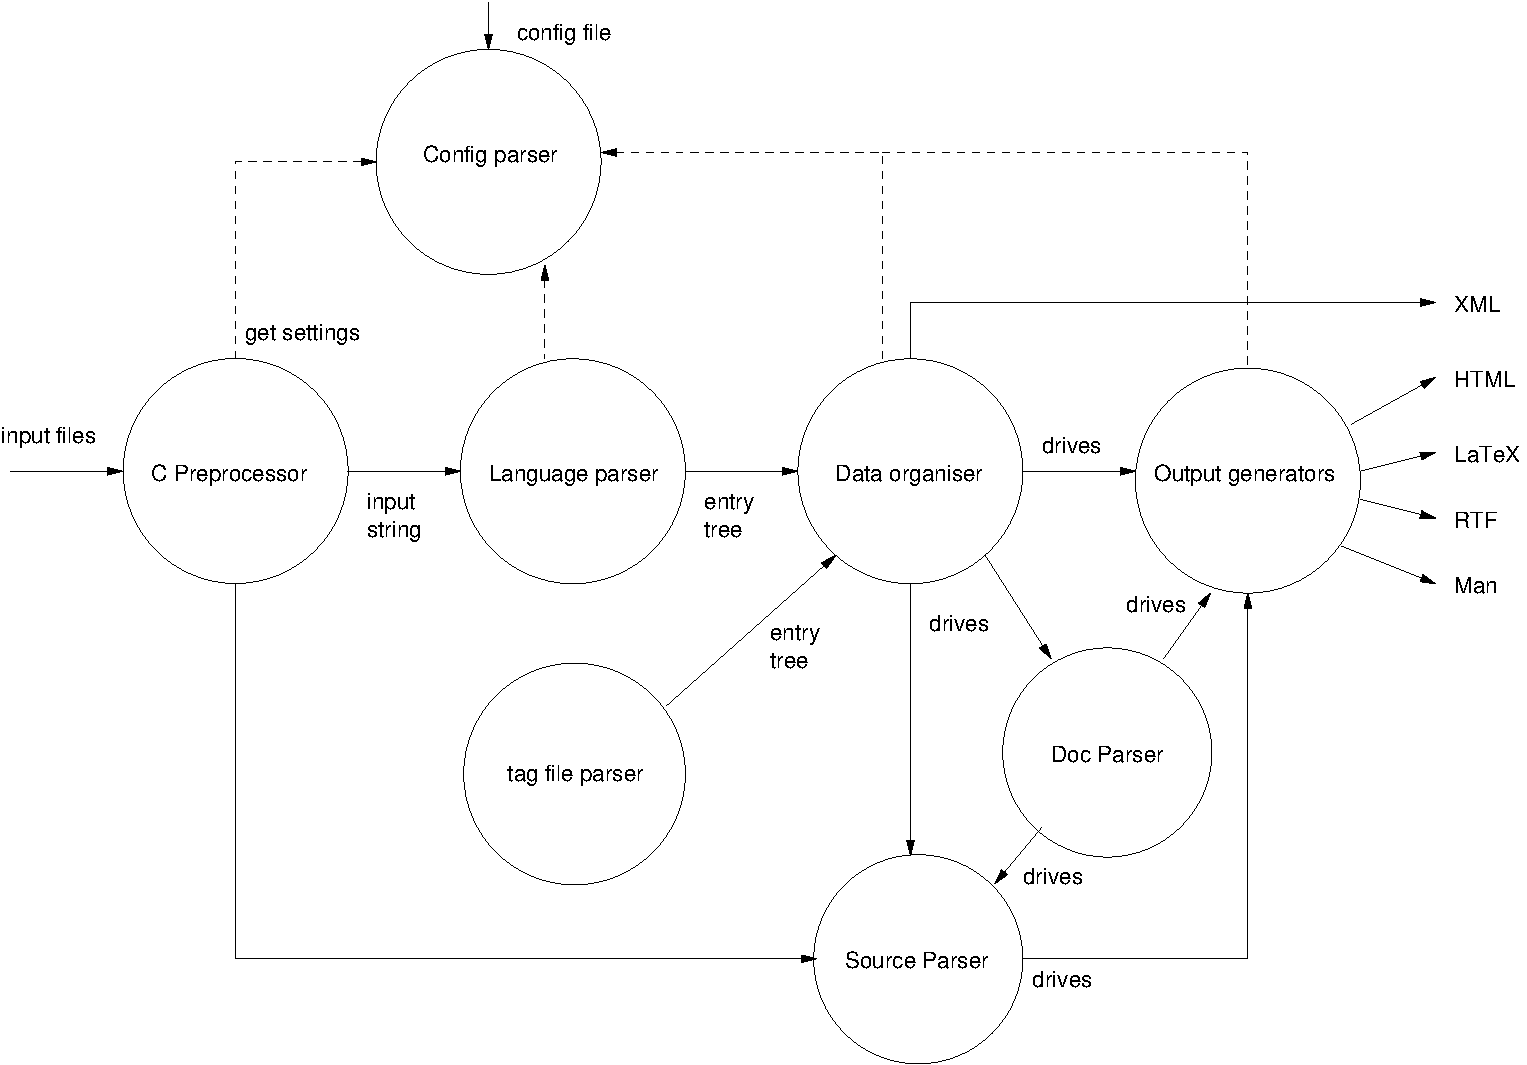
\includegraphics[width=14cm]{archoverview}\caption{Data flow overview}
\end{center}
\end{Image}


The following sections explain the steps above in more detail.

\subsubsection*{Config parser}

The configuration file that controls the settings of a project is parsed and the settings are stored in the singleton class {\tt Config} in {\tt src/config.h}. The parser itself is written using {\tt flex} and can be found in {\tt src/config.l}. This parser is also used directly by {\tt doxywizard}, so it is put in a separate library.

Each configuration option has one of 5 possible types: {\tt String}, {\tt List}, {\tt Enum}, {\tt Int}, or {\tt Bool}. The values of these options are available through the global functions {\tt Config\_\-getXXX()}, where {\tt XXX} is the type of the option. The argument of these function is a string naming the option as it appears in the configuration file. For instance: {\tt Config\_\-getBool}(\char`\"{}GENERATE\_\-TESTLIST\char`\"{}) returns a reference to a boolean value that is {\tt TRUE} if the test list was enabled in the config file.

The function {\tt readConfiguration()} in {\tt src/doxygen.cpp} reads the command line options and then calls the configuration parser.

\subsubsection*{C Preprocessor}

The input files mentioned in the config file are (by default) fed to the C Preprocessor (after being piped through a user defined filter if available).

The way the preprocessor works differs somewhat from a standard C Preprocessor. By default it does not do macro expansion, although it can be configured to expand all macros. Typical usage is to only expand a user specified set of macros. This is to allow macro names to appear in the type of function parameters for instance.

Another difference is that the preprocessor parses, but not actually includes code when it encounters a \#include (with the exception of \#include found inside \{ ... \} blocks). The reasons behind this deviation from the standard is to prevent feeding multiple definitions of the same functions/classes to doxygen's parser. If all source files would include a common header file for instance, the class and type definitions (and their documentation) would be present in each translation unit.

The preprocessor is written using {\tt flex} and can be found in {\tt src/pre.l}. For condition blocks (\#if) evaluation of constant expressions is needed. For this a {\tt yacc} based parser is used, which can be found in {\tt src/constexp.y} and {\tt src/constexp.l}.

The preprocessor is invoked for each file using the {\tt preprocessFile()} function declared in {\tt src/pre.h}, and will append the preprocessed result to a character buffer. The format of the character buffer is



\footnotesize\begin{verbatim}
0x06 file name 1 
0x06 preprocessed contents of file 1
...
0x06 file name n
0x06 preprocessed contents of file n
\end{verbatim}
\normalsize


\subsubsection*{Language parser}

The preprocessed input buffer is fed to the language parser, which is implemented as a big state machine using {\tt flex}. It can be found in the file {\tt src/scanner.l}. There is one parser for all languages (C/C++/Java/IDL). The state variables {\tt insideIDL} and {\tt insideJava} are uses at some places for language specific choices.

The task of the parser is to convert the input buffer into a tree of entries (basically an abstract syntax tree). An entry is defined in {\tt src/entry.h} and is a blob of loosely structured information. The most important field is {\tt section} which specifies the kind of information contained in the entry.

Possible improvements for future versions:\begin{itemize}
\item Use one scanner/parser per language instead of one big scanner.\item Move the first pass parsing of documentation blocks to a separate module.\item Parse defines (these are currently gathered by the preprocessor, and ignored by the language parser).\end{itemize}


\subsubsection*{Data organizer}

This step consists of many smaller steps, that build dictionaries of the extracted classes, files, namespaces, variables, functions, packages, pages, and groups. Besides building dictionaries, during this step relations (such as inheritance relations), between the extracted entities are computed.

Each step has a function defined in {\tt src/doxygen.cpp}, which operates on the tree of entries, built during language parsing. Look at the \char`\"{}Gathering information\char`\"{} part of {\tt parseInput()} for details.

The result of this step is a number of dictionaries, which can be found in the Doxygen \char`\"{}namespace\char`\"{} defined in {\tt src/doxygen.h}. Most elements of these dictionaries are derived from the class {\tt Definition}; The class {\tt MemberDef}, for instance, holds all information for a member. An instance of such a class can be part of a file ( class {\tt FileDef} ), a class ( class {\tt ClassDef} ), a namespace ( class {\tt NamespaceDef} ), a group ( class {\tt GroupDef} ), or a Java package ( class {\tt PackageDef} ).

\subsubsection*{Tag file parser}

If tag files are specified in the configuration file, these are parsed by a SAX based XML parser, which can be found in {\tt src/tagreader.cpp}. The result of parsing a tag file is the insertion of {\tt Entry} objects in the entry tree. The field {\tt Entry::tagInfo} is used to mark the entry as external, and holds information about the tag file.

\subsubsection*{Documentation parser}

Special comment blocks are stored as strings in the entities that they document. There is a string for the brief description and a string for the detailed description. The documentation parser reads these strings and executes the commands it finds in it (this is the second pass in parsing the documentation). It writes the result directly to the output generators.

The parser is written in C++ and can be found in src/docparser.cpp. The tokens that are eaten by the parser come from src/doctokenizer.l. Code fragments found in the comment blocks are passed on to the source parser.

The main entry point for the documentation parser is {\tt validatingParseDoc()} declared in {\tt src/docparser.h}. For simple texts with special commands {\tt validatingParseText()} is used.

\subsubsection*{Source parser}

If source browsing is enabled or if code fragments are encountered in the documentation, the source parser is invoked.

The code parser tries to cross-reference to source code it parses with documented entities. It also does syntax highlighting of the sources. The output is directly written to the output generators.

The main entry point for the code parser is {\tt parseCode()} declared in {\tt src/code.h}.

\subsubsection*{Output generators}

After data is gathered and cross-referenced, doxygen generates output in various formats. For this it uses the methods provided by the abstract class {\tt OutputGenerator}. In order to generate output for multiple formats at once, the methods of {\tt OutputList} are called instead. This class maintains a list of concrete output generators, where each method called is delegated to all generators in the list.

To allow small deviations in what is written to the output for each concrete output generator, it is possible to temporarily disable certain generators. The OutputList class contains various {\tt disable()} and {\tt enable()} methods for this. The methods {\tt OutputList::pushGeneratorState()} and {\tt OutputList::popGeneratorState()} are used to temporarily save the set of enabled/disabled output generators on a stack.

The XML is generated directly from the gathered data structures. In the future XML will be used as an intermediate language (IL). The output generators will then use this IL as a starting point to generate the specific output formats. The advantage of having an IL is that various independently developed tools written in various languages, could extract information from the XML output. Possible tools could be:\begin{itemize}
\item an interactive source browser\item a class diagram generator\item computing code metrics.\end{itemize}


\subsubsection*{Debugging}

Since doxygen uses a lot of {\tt flex} code it is important to understand how {\tt flex} works (for this one should read the man page) and to understand what it is doing when {\tt flex} is parsing some input. Fortunately, when flex is used with the -d option it outputs what rules matched. This makes it quite easy to follow what is going on for a particular input fragment.

To make it easier to toggle debug information for a given flex file I wrote the following perl script, which automatically adds or removes -d from the correct line in the Makefile:



\footnotesize\begin{verbatim}
#!/usr/local/bin/perl 

$file = shift @ARGV;
print "Toggle debugging mode for $file\n";

# add or remove the -d flex flag in the makefile
unless (rename "Makefile.libdoxygen","Makefile.libdoxygen.old") {
  print STDERR "Error: cannot rename Makefile.libdoxygen!\n";
  exit 1;
}
if (open(F,"<Makefile.libdoxygen.old")) {
  unless (open(G,">Makefile.libdoxygen")) {
    print STDERR "Error: opening file Makefile.libdoxygen for writing\n";
    exit 1; 
  }
  print "Processing Makefile.libdoxygen...\n";
  while (<F>) {
    if ( s/\(LEX\) -P([a-zA-Z]+)YY -t $file/(LEX) -d -P\1YY -t $file/g ) {
      print "Enabling debug info for $file\n";
    }
    elsif ( s/\(LEX\) -d -P([a-zA-Z]+)YY -t $file/(LEX) -P\1YY -t $file/g ) {
      print "Disabling debug info for $file\n";
    }
    print G "$_";
  }
  close F;
  unlink "Makefile.libdoxygen.old";
}
else {
  print STDERR "Warning file Makefile.libdoxygen.old does not exist!\n"; 
}

# touch the file
$now = time;
utime $now, $now, $file
\end{verbatim}
\normalsize
 
\index{perlmod@{perlmod}}

Since version 1.2.18, Doxygen can generate a new output format we have called the "Perl Module output format". It has been designed as an intermediate format that can be used to generate new and customized output without having to modify the Doxygen source. Therefore, its purpose is similar to the XML output format that can be also generated by Doxygen. The XML output format is more standard, but the Perl Module output format is possibly simpler and easier to use.

The Perl Module output format is still experimental at the moment and could be changed in incompatible ways in future versions, although this should not be very probable. It is also lacking some features of other Doxygen backends. However, it can be already used to generate useful output, as shown by the Perl Module-based LaTeX generator.

Please report any bugs or problems you find in the Perl Module backend or the Perl Module-based LaTeX generator to the doxygen-develop mailing list. Suggestions are welcome as well.\hypertarget{perlmod_using_perlmod_fmt}{}\section{Using the Perl Module output format.}\label{perlmod_using_perlmod_fmt}
When the {\bf GENERATE\_\-PERLMOD} tag is enabled in the Doxyfile, running Doxygen generates a number of files in the {\bf perlmod/} subdirectory of your output directory. These files are the following:

\begin{itemize}
\item {\bf DoxyDocs.pm}. This is the Perl module that actually contains the documentation, in the Perl Module format described \hyperlink{perlmod_doxydocs_format}{below}.

\item {\bf DoxyModel.pm}. This Perl module describes the structure of {\bf DoxyDocs.pm}, independently of the actual documentation. See \hyperlink{perlmod_doxymodel_format}{below} for details.

\item {\bf doxyrules.make}. This file contains the make rules to build and clean the files that are generated from the Doxyfile. Also contains the paths to those files and other relevant information. This file is intended to be included by your own Makefile.

\item {\bf Makefile}. This is a simple Makefile including {\bf doxyrules.make}.

\end{itemize}


To make use of the documentation stored in DoxyDocs.pm you can use one of the default Perl Module-based generators provided by Doxygen (at the moment this includes the Perl Module-based LaTeX generator, see \hyperlink{perlmod_perlmod_latex}{below}) or write your own customized generator. This should not be too hard if you have some knowledge of Perl and it's the main purpose of including the Perl Module backend in Doxygen. See \hyperlink{perlmod_doxydocs_format}{below} for details on how to do this.\hypertarget{perlmod_perlmod_latex}{}\section{Using the Perl Module-based LaTeX generator.}\label{perlmod_perlmod_latex}
The Perl Module-based LaTeX generator is pretty experimental and incomplete at the moment, but you could find it useful nevertheless. It can generate documentation for functions, typedefs and variables within files and classes and can be customized quite a lot by redefining TeX macros. However, there is still no documentation on how to do this.

Setting the {\bf PERLMOD\_\-LATEX} tag to {\bf YES} in the Doxyfile enables the creation of some additional files in the {\bf perlmod/} subdirectory of your output directory. These files contain the Perl scripts and LaTeX code necessary to generate PDF and DVI output from the Perl Module output, using PDFLaTeX and LaTeX respectively. Rules to automate the use of these files are also added to {\bf doxyrules.make} and the {\bf Makefile}.

The additional generated files are the following:

\begin{itemize}
\item {\bf doxylatex.pl}. This Perl script uses DoxyDocs.pm and DoxyModel.pm to generate {\bf doxydocs.tex}, a TeX file containing the documentation in a format that can be accessed by LaTeX code. This file is not directly LaTeXable.

\item {\bf doxyformat.tex}. This file contains the LaTeX code that transforms the documentation from doxydocs.tex into LaTeX text suitable to be LaTeX'ed and presented to the user.

\item {\bf doxylatex-template.pl}. This Perl script uses DoxyModel.pm to generate {\bf doxytemplate.tex}, a TeX file defining default values for some macros. doxytemplate.tex is included by doxyformat.tex to avoid the need of explicitly defining some macros.

\item {\bf doxylatex.tex}. This is a very simple LaTeX document that loads some packages and includes doxyformat.tex and doxydocs.tex. This document is LaTeX'ed to produce the PDF and DVI documentation by the rules added to {\bf doxyrules.make}.

\end{itemize}
\hypertarget{perlmod_pm_pdf_gen}{}\subsection{Simple creation of PDF and DVI output using the Perl Module-based LaTeX generator.}\label{perlmod_pm_pdf_gen}
To try this you need to have installed LaTeX, PDFLaTeX and the packages used by {\bf doxylatex.tex}.

\begin{enumerate}
\item Update your Doxyfile to the latest version using:

\small\begin{alltt}doxygen -u Doxyfile\end{alltt}
\normalsize 


\item Set both {\bf GENERATE\_\-PERLMOD} and {\bf PERLMOD\_\-LATEX} tags to YES in your Doxyfile.

\item Run Doxygen on your Doxyfile:

\small\begin{alltt}doxygen Doxyfile\end{alltt}
\normalsize 


\item A {\bf perlmod/} subdirectory should have appeared in your output directory. Enter the {\bf perlmod/} subdirectory and run:

\small\begin{alltt}make pdf\end{alltt}
\normalsize 




This should generate a {\bf doxylatex.pdf} with the documentation in PDF format.

\item Run:

\small\begin{alltt}make dvi\end{alltt}
\normalsize 




This should generate a {\bf doxylatex.dvi} with the documentation in DVI format.

\end{enumerate}
\hypertarget{perlmod_doxydocs_format}{}\section{Perl Module documentation format.}\label{perlmod_doxydocs_format}
The Perl Module documentation generated by Doxygen is stored in {\bf DoxyDocs.pm}. This is a very simple Perl module that contains only two statements: an assigment to the variable {\bf \$doxydocs} and the customary {\bf 1;} statement which usually ends Perl modules. The documentation is stored in the variable {\bf \$doxydocs}, which can then be accessed by a Perl script using {\bf DoxyDocs.pm}.

{\bf \$doxydocs} contains a tree-like structure composed of three types of nodes: strings, hashes and lists.

\begin{itemize}
\item {\bf Strings}. These are normal Perl strings. They can be of any length can contain any character. Their semantics depends on their location within the tree. This type of node has no children.

\item {\bf Hashes}. These are references to anonymous Perl hashes. A hash can have multiple fields, each with a different key. The value of a hash field can be a string, a hash or a list, and its semantics depends on the key of the hash field and the location of the hash within the tree. The values of the hash fields are the children of the node.

\item {\bf Lists}. These are references to anonymous Perl lists. A list has an undefined number of elements, which are the children of the node. Each element has the same type (string, hash or list) and the same semantics, depending on the location of the list within the tree.

\end{itemize}


As you can see, the documentation contained in {\bf \$doxydocs} does not present any special impediment to be processed by a simple Perl script. To be able to generate meaningful output using the documentation contained in {\bf \$doxydocs} you'll probably need to know the semantics of the nodes of the documentation tree, which we present in \hyperlink{perlmod_tree}{this page}.\hypertarget{perlmod_doxymodel_format}{}\section{Data structure describing the Perl Module documentation tree.}\label{perlmod_doxymodel_format}
You might be interested in processing the documentation contained in {\bf DoxyDocs.pm} without needing to take into account the semantics of each node of the documentation tree. For this purpose, Doxygen generates a {\bf DoxyModel.pm} file which contains a data structure describing the type and children of each node in the documentation tree.

The rest of this section is to be written yet, but in the meantime you can look at the Perl scripts generated by Doxygen (such as {\bf doxylatex.pl} or {\bf doxytemplate-latex.pl}) to get an idea on how to use {\bf DoxyModel.pm}. 
%\subsection*{Nodes in the documentation tree of the Perl Module output format.}

This is a description of the structure of the documentation tree in {\bf DoxyDocs.pm}. Each item in the list below describes a node in the tree, and the format of the description is as follows:

\begin{itemize}
\item \mbox{[} key =$>$ \mbox{]} {\bf Name} {\em (type)\/}. Explanation of the content. \end{itemize}


Where

\begin{itemize}
\item The \char`\"{}key =\&gt;\char`\"{} part only appears if the parent node is a hash. \char`\"{}key\char`\"{} is the key for this node.

\item {\bf \char`\"{}Name\char`\"{}} is a unique name for the node, defined in DoxyModel.pm.

\item {\em \char`\"{}(type)\char`\"{}\/} is the type of the node: \char`\"{}string\char`\"{} for string nodes, \char`\"{}hash\char`\"{} for hash nodes, \char`\"{}list\char`\"{} for list nodes, and \char`\"{}doc\char`\"{} for documentation subtrees. The structure of documentation subtrees is not described anywhere yet, but you can look for example at {\bf doxylatex.pl} to see how to process it.

\end{itemize}


The meaning of each node in the documentation tree is as follows: \begin{itemize}
\item {\bf Root} {\em (hash)\/}. Root node. \begin{itemize}
\item classes =$>$ {\bf Classes} {\em (list)\/}. Documented classes. \begin{itemize}
\item {\bf Class} {\em (hash)\/}. A documented class. \begin{itemize}
\item protected\_\-members =$>$ {\bf ClassProtectedMembers} {\em (hash)\/}. Information about the protected members in the class. \begin{itemize}
\item members =$>$ {\bf ClassProtectedMemberList} {\em (list)\/}. protected member list. \begin{itemize}
\item {\bf ClassProtectedMember} {\em (hash)\/}. A protected member. \begin{itemize}
\item protection =$>$ {\bf ClassProtectedMemberProtection} {\em (string)\/}. Protection of the protected member. \item detailed =$>$ {\bf ClassProtectedMemberDetailed} {\em (hash)\/}. Detailed information about the protected member. \begin{itemize}
\item doc =$>$ {\bf ClassProtectedMemberDetailedDoc} {\em (doc)\/}. Detailed documentation for the protected member. \item see =$>$ {\bf ClassProtectedMemberSee} {\em (doc)\/}. \char`\"{}See also\char`\"{} documentation for the protected member. \end{itemize}
\item kind =$>$ {\bf ClassProtectedMemberKind} {\em (string)\/}. Kind of protected member (usually \char`\"{}variable\char`\"{}). \item name =$>$ {\bf ClassProtectedMemberName} {\em (string)\/}. Name of the protected member. \item type =$>$ {\bf ClassProtectedMemberType} {\em (string)\/}. Data type of the protected member. \end{itemize}
\end{itemize}
\end{itemize}
\item detailed =$>$ {\bf ClassDetailed} {\em (hash)\/}. Detailed information about the class. \begin{itemize}
\item doc =$>$ {\bf ClassDetailedDoc} {\em (doc)\/}. Detailed documentation block for the class. \end{itemize}
\item protected\_\-typedefs =$>$ {\bf ClassProtectedTypedefs} {\em (hash)\/}. Information about the protected typedefs in the class. \begin{itemize}
\item members =$>$ {\bf ClassProtectedTypedefList} {\em (list)\/}. protected typedef list. \begin{itemize}
\item {\bf ClassProtectedTypedef} {\em (hash)\/}. A protected typedef. \begin{itemize}
\item protection =$>$ {\bf ClassProtectedTypedefProtection} {\em (string)\/}. Protection of the protected typedef. \item detailed =$>$ {\bf ClassProtectedTypedefDetailed} {\em (hash)\/}. Detailed information about the protected typedef. \begin{itemize}
\item doc =$>$ {\bf ClassProtectedTypedefDetailedDoc} {\em (doc)\/}. Detailed documentation for the protected typedef. \item see =$>$ {\bf ClassProtectedTypedefSee} {\em (doc)\/}. \char`\"{}See also\char`\"{} documentation for the protected typedef. \end{itemize}
\item kind =$>$ {\bf ClassProtectedTypedefKind} {\em (string)\/}. Kind of protected typedef (usually \char`\"{}typedef\char`\"{}). \item name =$>$ {\bf ClassProtectedTypedefName} {\em (string)\/}. Name of the protected typedef. \item type =$>$ {\bf ClassProtectedTypedefType} {\em (string)\/}. Data type of the protected typedef. \end{itemize}
\end{itemize}
\end{itemize}
\item name =$>$ {\bf ClassName} {\em (string)\/}. Name of the class. \item private\_\-members =$>$ {\bf ClassPrivateMembers} {\em (hash)\/}. Information about the private members in the class. \begin{itemize}
\item members =$>$ {\bf ClassPrivateMemberList} {\em (list)\/}. private member list. \begin{itemize}
\item {\bf ClassPrivateMember} {\em (hash)\/}. A private member. \begin{itemize}
\item protection =$>$ {\bf ClassPrivateMemberProtection} {\em (string)\/}. Protection of the private member. \item detailed =$>$ {\bf ClassPrivateMemberDetailed} {\em (hash)\/}. Detailed information about the private member. \begin{itemize}
\item doc =$>$ {\bf ClassPrivateMemberDetailedDoc} {\em (doc)\/}. Detailed documentation for the private member. \item see =$>$ {\bf ClassPrivateMemberSee} {\em (doc)\/}. \char`\"{}See also\char`\"{} documentation for the private member. \end{itemize}
\item kind =$>$ {\bf ClassPrivateMemberKind} {\em (string)\/}. Kind of private member (usually \char`\"{}variable\char`\"{}). \item name =$>$ {\bf ClassPrivateMemberName} {\em (string)\/}. Name of the private member. \item type =$>$ {\bf ClassPrivateMemberType} {\em (string)\/}. Data type of the private member. \end{itemize}
\end{itemize}
\end{itemize}
\item private\_\-typedefs =$>$ {\bf ClassPrivateTypedefs} {\em (hash)\/}. Information about the private typedefs in the class. \begin{itemize}
\item members =$>$ {\bf ClassPrivateTypedefList} {\em (list)\/}. private typedef list. \begin{itemize}
\item {\bf ClassPrivateTypedef} {\em (hash)\/}. A private typedef. \begin{itemize}
\item protection =$>$ {\bf ClassPrivateTypedefProtection} {\em (string)\/}. Protection of the private typedef. \item detailed =$>$ {\bf ClassPrivateTypedefDetailed} {\em (hash)\/}. Detailed information about the private typedef. \begin{itemize}
\item doc =$>$ {\bf ClassPrivateTypedefDetailedDoc} {\em (doc)\/}. Detailed documentation for the private typedef. \item see =$>$ {\bf ClassPrivateTypedefSee} {\em (doc)\/}. \char`\"{}See also\char`\"{} documentation for the private typedef. \end{itemize}
\item kind =$>$ {\bf ClassPrivateTypedefKind} {\em (string)\/}. Kind of private typedef (usually \char`\"{}typedef\char`\"{}). \item name =$>$ {\bf ClassPrivateTypedefName} {\em (string)\/}. Name of the private typedef. \item type =$>$ {\bf ClassPrivateTypedefType} {\em (string)\/}. Data type of the private typedef. \end{itemize}
\end{itemize}
\end{itemize}
\item protected\_\-methods =$>$ {\bf ClassProtectedMethods} {\em (hash)\/}. Information about the protected methods in the class. \begin{itemize}
\item members =$>$ {\bf ClassProtectedMethodList} {\em (list)\/}. protected method list. \begin{itemize}
\item {\bf ClassProtectedMethod} {\em (hash)\/}. A protected method. \begin{itemize}
\item parameters =$>$ {\bf ClassProtectedMethodParams} {\em (list)\/}. List of the parameters of the protected method. \begin{itemize}
\item {\bf ClassProtectedMethodParam} {\em (hash)\/}. A parameter of the protected method. \begin{itemize}
\item declaration\_\-name =$>$ {\bf ClassProtectedMethodParamName} {\em (string)\/}. The name of the parameter. \item type =$>$ {\bf ClassProtectedMethodParamType} {\em (string)\/}. The data type of the parameter. \end{itemize}
\end{itemize}
\item protection =$>$ {\bf ClassProtectedMethodProtection} {\em (string)\/}. Protection of the protected method. \item virtualness =$>$ {\bf ClassProtectedMethodVirtualness} {\em (string)\/}. Virtualness of the protected method. \item detailed =$>$ {\bf ClassProtectedMethodDetailed} {\em (hash)\/}. Detailed information about the protected method. \begin{itemize}
\item params =$>$ {\bf ClassProtectedMethodPDBlocks} {\em (list)\/}. List of parameter documentation blocks for the protected method. \begin{itemize}
\item {\bf ClassProtectedMethodPDBlock} {\em (hash)\/}. A parameter documentation block for the protected method. \begin{itemize}
\item parameters =$>$ {\bf ClassProtectedMethodPDParams} {\em (list)\/}. Parameter list for this parameter documentation block. \begin{itemize}
\item {\bf ClassProtectedMethodPDParam} {\em (hash)\/}. A parameter documented by this documentation block. \begin{itemize}
\item name =$>$ {\bf ClassProtectedMethodPDParamName} {\em (string)\/}. Name of the parameter. \end{itemize}
\end{itemize}
\item doc =$>$ {\bf ClassProtectedMethodPDDoc} {\em (doc)\/}. Documentation for this parameter documentation block. \end{itemize}
\end{itemize}
\item doc =$>$ {\bf ClassProtectedMethodDetailedDoc} {\em (doc)\/}. Detailed documentation for the protected method. \item see =$>$ {\bf ClassProtectedMethodSee} {\em (doc)\/}. \char`\"{}See also\char`\"{} documentation for the protected method. \item return =$>$ {\bf ClassProtectedMethodReturn} {\em (doc)\/}. Documentation about the return value of the protected method. \end{itemize}
\item kind =$>$ {\bf ClassProtectedMethodKind} {\em (string)\/}. Kind of protected method (usually \char`\"{}function\char`\"{}). \item name =$>$ {\bf ClassProtectedMethodName} {\em (string)\/}. Name of the protected method. \item type =$>$ {\bf ClassProtectedMethodType} {\em (string)\/}. Data type returned by the protected method. \item static =$>$ {\bf ClassProtectedMethodStatic} {\em (string)\/}. Whether the protected method is static. \end{itemize}
\end{itemize}
\end{itemize}
\item public\_\-typedefs =$>$ {\bf ClassPublicTypedefs} {\em (hash)\/}. Information about the public typedefs in the class. \begin{itemize}
\item members =$>$ {\bf ClassPublicTypedefList} {\em (list)\/}. public typedef list. \begin{itemize}
\item {\bf ClassPublicTypedef} {\em (hash)\/}. A public typedef. \begin{itemize}
\item protection =$>$ {\bf ClassPublicTypedefProtection} {\em (string)\/}. Protection of the public typedef. \item detailed =$>$ {\bf ClassPublicTypedefDetailed} {\em (hash)\/}. Detailed information about the public typedef. \begin{itemize}
\item doc =$>$ {\bf ClassPublicTypedefDetailedDoc} {\em (doc)\/}. Detailed documentation for the public typedef. \item see =$>$ {\bf ClassPublicTypedefSee} {\em (doc)\/}. \char`\"{}See also\char`\"{} documentation for the public typedef. \end{itemize}
\item kind =$>$ {\bf ClassPublicTypedefKind} {\em (string)\/}. Kind of public typedef (usually \char`\"{}typedef\char`\"{}). \item name =$>$ {\bf ClassPublicTypedefName} {\em (string)\/}. Name of the public typedef. \item type =$>$ {\bf ClassPublicTypedefType} {\em (string)\/}. Data type of the public typedef. \end{itemize}
\end{itemize}
\end{itemize}
\item public\_\-members =$>$ {\bf ClassPublicMembers} {\em (hash)\/}. Information about the public members in the class. \begin{itemize}
\item members =$>$ {\bf ClassPublicMemberList} {\em (list)\/}. public member list. \begin{itemize}
\item {\bf ClassPublicMember} {\em (hash)\/}. A public member. \begin{itemize}
\item protection =$>$ {\bf ClassPublicMemberProtection} {\em (string)\/}. Protection of the public member. \item detailed =$>$ {\bf ClassPublicMemberDetailed} {\em (hash)\/}. Detailed information about the public member. \begin{itemize}
\item doc =$>$ {\bf ClassPublicMemberDetailedDoc} {\em (doc)\/}. Detailed documentation for the public member. \item see =$>$ {\bf ClassPublicMemberSee} {\em (doc)\/}. \char`\"{}See also\char`\"{} documentation for the public member. \end{itemize}
\item kind =$>$ {\bf ClassPublicMemberKind} {\em (string)\/}. Kind of public member (usually \char`\"{}variable\char`\"{}). \item name =$>$ {\bf ClassPublicMemberName} {\em (string)\/}. Name of the public member. \item type =$>$ {\bf ClassPublicMemberType} {\em (string)\/}. Data type of the public member. \end{itemize}
\end{itemize}
\end{itemize}
\item private\_\-methods =$>$ {\bf ClassPrivateMethods} {\em (hash)\/}. Information about the private methods in the class. \begin{itemize}
\item members =$>$ {\bf ClassPrivateMethodList} {\em (list)\/}. private method list. \begin{itemize}
\item {\bf ClassPrivateMethod} {\em (hash)\/}. A private method. \begin{itemize}
\item parameters =$>$ {\bf ClassPrivateMethodParams} {\em (list)\/}. List of the parameters of the private method. \begin{itemize}
\item {\bf ClassPrivateMethodParam} {\em (hash)\/}. A parameter of the private method. \begin{itemize}
\item declaration\_\-name =$>$ {\bf ClassPrivateMethodParamName} {\em (string)\/}. The name of the parameter. \item type =$>$ {\bf ClassPrivateMethodParamType} {\em (string)\/}. The data type of the parameter. \end{itemize}
\end{itemize}
\item protection =$>$ {\bf ClassPrivateMethodProtection} {\em (string)\/}. Protection of the private method. \item virtualness =$>$ {\bf ClassPrivateMethodVirtualness} {\em (string)\/}. Virtualness of the private method. \item detailed =$>$ {\bf ClassPrivateMethodDetailed} {\em (hash)\/}. Detailed information about the private method. \begin{itemize}
\item params =$>$ {\bf ClassPrivateMethodPDBlocks} {\em (list)\/}. List of parameter documentation blocks for the private method. \begin{itemize}
\item {\bf ClassPrivateMethodPDBlock} {\em (hash)\/}. A parameter documentation block for the private method. \begin{itemize}
\item parameters =$>$ {\bf ClassPrivateMethodPDParams} {\em (list)\/}. Parameter list for this parameter documentation block. \begin{itemize}
\item {\bf ClassPrivateMethodPDParam} {\em (hash)\/}. A parameter documented by this documentation block. \begin{itemize}
\item name =$>$ {\bf ClassPrivateMethodPDParamName} {\em (string)\/}. Name of the parameter. \end{itemize}
\end{itemize}
\item doc =$>$ {\bf ClassPrivateMethodPDDoc} {\em (doc)\/}. Documentation for this parameter documentation block. \end{itemize}
\end{itemize}
\item doc =$>$ {\bf ClassPrivateMethodDetailedDoc} {\em (doc)\/}. Detailed documentation for the private method. \item see =$>$ {\bf ClassPrivateMethodSee} {\em (doc)\/}. \char`\"{}See also\char`\"{} documentation for the private method. \item return =$>$ {\bf ClassPrivateMethodReturn} {\em (doc)\/}. Documentation about the return value of the private method. \end{itemize}
\item kind =$>$ {\bf ClassPrivateMethodKind} {\em (string)\/}. Kind of private method (usually \char`\"{}function\char`\"{}). \item name =$>$ {\bf ClassPrivateMethodName} {\em (string)\/}. Name of the private method. \item type =$>$ {\bf ClassPrivateMethodType} {\em (string)\/}. Data type returned by the private method. \item static =$>$ {\bf ClassPrivateMethodStatic} {\em (string)\/}. Whether the private method is static. \end{itemize}
\end{itemize}
\end{itemize}
\item public\_\-methods =$>$ {\bf ClassPublicMethods} {\em (hash)\/}. Information about the public methods in the class. \begin{itemize}
\item members =$>$ {\bf ClassPublicMethodList} {\em (list)\/}. public method list. \begin{itemize}
\item {\bf ClassPublicMethod} {\em (hash)\/}. A public method. \begin{itemize}
\item parameters =$>$ {\bf ClassPublicMethodParams} {\em (list)\/}. List of the parameters of the public method. \begin{itemize}
\item {\bf ClassPublicMethodParam} {\em (hash)\/}. A parameter of the public method. \begin{itemize}
\item declaration\_\-name =$>$ {\bf ClassPublicMethodParamName} {\em (string)\/}. The name of the parameter. \item type =$>$ {\bf ClassPublicMethodParamType} {\em (string)\/}. The data type of the parameter. \end{itemize}
\end{itemize}
\item protection =$>$ {\bf ClassPublicMethodProtection} {\em (string)\/}. Protection of the public method. \item virtualness =$>$ {\bf ClassPublicMethodVirtualness} {\em (string)\/}. Virtualness of the public method. \item detailed =$>$ {\bf ClassPublicMethodDetailed} {\em (hash)\/}. Detailed information about the public method. \begin{itemize}
\item params =$>$ {\bf ClassPublicMethodPDBlocks} {\em (list)\/}. List of parameter documentation blocks for the public method. \begin{itemize}
\item {\bf ClassPublicMethodPDBlock} {\em (hash)\/}. A parameter documentation block for the public method. \begin{itemize}
\item parameters =$>$ {\bf ClassPublicMethodPDParams} {\em (list)\/}. Parameter list for this parameter documentation block. \begin{itemize}
\item {\bf ClassPublicMethodPDParam} {\em (hash)\/}. A parameter documented by this documentation block. \begin{itemize}
\item name =$>$ {\bf ClassPublicMethodPDParamName} {\em (string)\/}. Name of the parameter. \end{itemize}
\end{itemize}
\item doc =$>$ {\bf ClassPublicMethodPDDoc} {\em (doc)\/}. Documentation for this parameter documentation block. \end{itemize}
\end{itemize}
\item doc =$>$ {\bf ClassPublicMethodDetailedDoc} {\em (doc)\/}. Detailed documentation for the public method. \item see =$>$ {\bf ClassPublicMethodSee} {\em (doc)\/}. \char`\"{}See also\char`\"{} documentation for the public method. \item return =$>$ {\bf ClassPublicMethodReturn} {\em (doc)\/}. Documentation about the return value of the public method. \end{itemize}
\item kind =$>$ {\bf ClassPublicMethodKind} {\em (string)\/}. Kind of public method (usually \char`\"{}function\char`\"{}). \item name =$>$ {\bf ClassPublicMethodName} {\em (string)\/}. Name of the public method. \item type =$>$ {\bf ClassPublicMethodType} {\em (string)\/}. Data type returned by the public method. \item static =$>$ {\bf ClassPublicMethodStatic} {\em (string)\/}. Whether the public method is static. \end{itemize}
\end{itemize}
\end{itemize}
\end{itemize}
\end{itemize}
\item files =$>$ {\bf Files} {\em (list)\/}. Documented files. \begin{itemize}
\item {\bf File} {\em (hash)\/}. A documented file. \begin{itemize}
\item detailed =$>$ {\bf FileDetailed} {\em (hash)\/}. Detailed information about the file. \begin{itemize}
\item doc =$>$ {\bf FileDetailedDoc} {\em (doc)\/}. Detailed documentation block for the file. \end{itemize}
\item functions =$>$ {\bf FileFunctions} {\em (hash)\/}. Information about the functions in the file. \begin{itemize}
\item members =$>$ {\bf FileFunctionList} {\em (list)\/}. function list. \begin{itemize}
\item {\bf FileFunction} {\em (hash)\/}. A function. \begin{itemize}
\item parameters =$>$ {\bf FileFunctionParams} {\em (list)\/}. List of the parameters of the function. \begin{itemize}
\item {\bf FileFunctionParam} {\em (hash)\/}. A parameter of the function. \begin{itemize}
\item declaration\_\-name =$>$ {\bf FileFunctionParamName} {\em (string)\/}. The name of the parameter. \item type =$>$ {\bf FileFunctionParamType} {\em (string)\/}. The data type of the parameter. \end{itemize}
\end{itemize}
\item protection =$>$ {\bf FileFunctionProtection} {\em (string)\/}. Protection of the function. \item virtualness =$>$ {\bf FileFunctionVirtualness} {\em (string)\/}. Virtualness of the function. \item detailed =$>$ {\bf FileFunctionDetailed} {\em (hash)\/}. Detailed information about the function. \begin{itemize}
\item params =$>$ {\bf FileFunctionPDBlocks} {\em (list)\/}. List of parameter documentation blocks for the function. \begin{itemize}
\item {\bf FileFunctionPDBlock} {\em (hash)\/}. A parameter documentation block for the function. \begin{itemize}
\item parameters =$>$ {\bf FileFunctionPDParams} {\em (list)\/}. Parameter list for this parameter documentation block. \begin{itemize}
\item {\bf FileFunctionPDParam} {\em (hash)\/}. A parameter documented by this documentation block. \begin{itemize}
\item name =$>$ {\bf FileFunctionPDParamName} {\em (string)\/}. Name of the parameter. \end{itemize}
\end{itemize}
\item doc =$>$ {\bf FileFunctionPDDoc} {\em (doc)\/}. Documentation for this parameter documentation block. \end{itemize}
\end{itemize}
\item doc =$>$ {\bf FileFunctionDetailedDoc} {\em (doc)\/}. Detailed documentation for the function. \item see =$>$ {\bf FileFunctionSee} {\em (doc)\/}. \char`\"{}See also\char`\"{} documentation for the function. \item return =$>$ {\bf FileFunctionReturn} {\em (doc)\/}. Documentation about the return value of the function. \end{itemize}
\item kind =$>$ {\bf FileFunctionKind} {\em (string)\/}. Kind of function (usually \char`\"{}function\char`\"{}). \item name =$>$ {\bf FileFunctionName} {\em (string)\/}. Name of the function. \item type =$>$ {\bf FileFunctionType} {\em (string)\/}. Data type returned by the function. \item static =$>$ {\bf FileFunctionStatic} {\em (string)\/}. Whether the function is static. \end{itemize}
\end{itemize}
\end{itemize}
\item name =$>$ {\bf FileName} {\em (string)\/}. Name of the file. \item variables =$>$ {\bf FileVariables} {\em (hash)\/}. Information about the variables in the file. \begin{itemize}
\item members =$>$ {\bf FileVariableList} {\em (list)\/}. variable list. \begin{itemize}
\item {\bf FileVariable} {\em (hash)\/}. A variable. \begin{itemize}
\item protection =$>$ {\bf FileVariableProtection} {\em (string)\/}. Protection of the variable. \item detailed =$>$ {\bf FileVariableDetailed} {\em (hash)\/}. Detailed information about the variable. \begin{itemize}
\item doc =$>$ {\bf FileVariableDetailedDoc} {\em (doc)\/}. Detailed documentation for the variable. \item see =$>$ {\bf FileVariableSee} {\em (doc)\/}. \char`\"{}See also\char`\"{} documentation for the variable. \end{itemize}
\item kind =$>$ {\bf FileVariableKind} {\em (string)\/}. Kind of variable (usually \char`\"{}variable\char`\"{}). \item name =$>$ {\bf FileVariableName} {\em (string)\/}. Name of the variable. \item type =$>$ {\bf FileVariableType} {\em (string)\/}. Data type of the variable. \end{itemize}
\end{itemize}
\end{itemize}
\item typedefs =$>$ {\bf FileTypedefs} {\em (hash)\/}. Information about the typedefs in the file. \begin{itemize}
\item members =$>$ {\bf FileTypedefList} {\em (list)\/}. typedef list. \begin{itemize}
\item {\bf FileTypedef} {\em (hash)\/}. A typedef. \begin{itemize}
\item protection =$>$ {\bf FileTypedefProtection} {\em (string)\/}. Protection of the typedef. \item detailed =$>$ {\bf FileTypedefDetailed} {\em (hash)\/}. Detailed information about the typedef. \begin{itemize}
\item doc =$>$ {\bf FileTypedefDetailedDoc} {\em (doc)\/}. Detailed documentation for the typedef. \item see =$>$ {\bf FileTypedefSee} {\em (doc)\/}. \char`\"{}See also\char`\"{} documentation for the typedef. \end{itemize}
\item kind =$>$ {\bf FileTypedefKind} {\em (string)\/}. Kind of typedef (usually \char`\"{}typedef\char`\"{}). \item name =$>$ {\bf FileTypedefName} {\em (string)\/}. Name of the typedef. \item type =$>$ {\bf FileTypedefType} {\em (string)\/}. Data type of the typedef. \end{itemize}
\end{itemize}
\end{itemize}
\end{itemize}
\end{itemize}
\end{itemize}
\end{itemize}

\subsubsection*{Support for multiple languages}

Doxygen has built-in support for multiple languages. This means that the text fragments, generated by doxygen, can be produced in languages other than English (the default). The output language is chosen through the configuration file (with default name and known as Doxyfile).

Currently (version 1.5.5), 34 languages are supported (sorted alphabetically): Afrikaans, Arabic, Brazilian Portuguese, Catalan, Chinese, Chinese Traditional, Croatian, Czech, Danish, Dutch, English, Finnish, French, German, Greek, Hungarian, Indonesian, Italian, Japanese (+En), Korean (+En), Lithuanian, Macedonian, Norwegian, Persian, Polish, Portuguese, Romanian, Russian, Serbian, Slovak, Slovene, Spanish, Swedish, and Ukrainian..

The table of information related to the supported languages follows. It is sorted by language alphabetically. The {\bf Status} column was generated from sources and shows approximately the last version when the translator was updated.



 
\begin{tabular}{|l|l|l|l|}
  \hline 
  {\bf Language} & {\bf Maintainer} & {\bf Contact address} & {\bf Status} \\
  \hline

  \hline
  Afrikaans & Johan Prinsloo & {\tt\tiny johan@zippysnoek.com} & 1.4.6 \\
  \hline
  Arabic & Moaz Reyad & {\tt\tiny moazreyad@yahoo.com} & 1.4.6 \\
  \hline
  Brazilian Portuguese & Fabio "FJTC" Jun Takada Chino & {\tt\tiny jun-chino@uol.com.br} & up-to-date \\
  \hline
  Catalan & Maximiliano Pin & {\tt\tiny mcpin@emtesistemas.com} & 1.5.4 \\
  ~ & Albert Mora & {\tt\tiny amora@iua.upf.es} & ~ \\
  \hline
  Chinese & Li Daobing & {\tt\tiny lidaobing@gmail.com} & up-to-date \\
  ~ & Wei Liu & {\tt\tiny liuwei@asiainfo.com} & ~ \\
  \hline
  Chinese Traditional & Daniel YC Lin & {\tt\tiny dlin.tw@gmail.com} & up-to-date \\
  ~ & Gary Lee & {\tt\tiny garywlee@gmail.com} & ~ \\
  \hline
  Croatian & Boris Bralo & {\tt\tiny boris.bralo@zg.htnet.hr} & up-to-date \\
  \hline
  Czech & Petr P\v{r}ikryl & {\tt\tiny prikrylp@skil.cz} & up-to-date \\
  \hline
  Danish & Erik S\o{}e S\o{}rensen & {\tt\tiny eriksoe+doxygen@daimi.au.dk} & 1.5.4 \\
  \hline
  Dutch & Dimitri van Heesch & {\tt\tiny dimitri@stack.nl} & up-to-date \\
  \hline
  English & Dimitri van Heesch & {\tt\tiny dimitri@stack.nl} & up-to-date \\
  \hline
  Finnish & Olli Korhonen & {\tt\tiny olli.korhonen lost@cyberspace} & obsolete \\
  \hline
  French & Xavier Outhier & {\tt\tiny xouthier@yahoo.fr} & 1.5.4 \\
  \hline
  German & Jens Seidel & {\tt\tiny jensseidel@users.sf.net} & up-to-date \\
  \hline
  Greek & Paul Gessos & {\tt\tiny nickreserved@yahoo.com} & 1.5.4 \\
  \hline
  Hungarian & \'{A}kos Kiss & {\tt\tiny akiss@users.sourceforge.net} & 1.4.6 \\
  ~ & F\"{o}ldv\'{a}ri Gy\"{o}rgy & {\tt\tiny foldvari lost@cyberspace} & ~ \\
  \hline
  Indonesian & Hendy Irawan & {\tt\tiny ceefour@gauldong.net} & 1.4.6 \\
  \hline
  Italian & Alessandro Falappa & {\tt\tiny alessandro@falappa.net} & up-to-date \\
  ~ & Ahmed Aldo Faisal & {\tt\tiny aaf23@cam.ac.uk} & ~ \\
  \hline
  Japanese & Ryunosuke Satoh & {\tt\tiny sun594@hotmail.com} & 1.5.4 \\
  ~ & Kenji Nagamatsu & {\tt\tiny naga@joyful.club.ne.jp} & ~ \\
  ~ & Iwasa Kazmi & {\tt\tiny iwasa@cosmo-system.jp} & ~ \\
  \hline
  JapaneseEn & see the Japanese language & {\tt\tiny ~} & English based \\
  \hline
  Korean & Kim Taedong & {\tt\tiny fly1004@gmail.com} & up-to-date \\
  ~ & SooYoung Jung & {\tt\tiny jung5000@gmail.com} & ~ \\
  ~ & Richard Kim & {\tt\tiny ryk@dspwiz.com} & ~ \\
  \hline
  KoreanEn & see the Korean language & {\tt\tiny ~} & English based \\
  \hline
  Lithuanian & Tomas Simonaitis & {\tt\tiny haden@homelan.lt} & 1.4.6 \\
  ~ & Mindaugas Radzius & {\tt\tiny mindaugasradzius@takas.lt} & ~ \\
  ~ & Aidas Berukstis & {\tt\tiny aidasber@takas.lt} & ~ \\
  \hline
  Macedonian & Slave Jovanovski & {\tt\tiny slavejovanovski@yahoo.com} & 1.5.04 \\
  \hline
  Norwegian & Lars Erik Jordet & {\tt\tiny lejordet@gmail.com} & 1.4.6 \\
  \hline
  Persian & Ali Nadalizadeh & {\tt\tiny nadalizadeh@gmail.com} & up-to-date \\
  \hline
  Polish & Piotr Kaminski & {\tt\tiny Piotr.Kaminski@ctm.gdynia.pl} & 1.4.6 \\
  ~ & Grzegorz Kowal & {\tt\tiny g\_kowal@poczta.onet.pl} & ~ \\
  \hline
  Portuguese & Rui Godinho Lopes & {\tt\tiny ruiglopes@yahoo.com} & 1.3.3 \\
  \hline
  Romanian & Alexandru Iosup & {\tt\tiny aiosup@yahoo.com} & 1.4.1 \\
  \hline
  Russian & Alexandr Chelpanov & {\tt\tiny cav@cryptopro.ru} & 1.5.4 \\
  \hline
  Serbian & Dejan Milosavljevic & {\tt\tiny dmilos@email.com} & 1.4.1 \\
  \hline
  Slovak & Stanislav Kudl\'{a}\v{c} & {\tt\tiny skudlac@pobox.sk} & 1.2.18 \\
  \hline
  Slovene & Matja\v{z} Ostrover\v{s}nik & {\tt\tiny matjaz.ostroversnik@ostri.org} & 1.4.6 \\
  \hline
  Spanish & Bartomeu & {\tt\tiny bartomeu@loteria3cornella.com} & up-to-date \\
  ~ & Francisco Oltra Thennet & {\tt\tiny foltra@puc.cl} & ~ \\
  \hline
  Swedish & Mikael Hallin & {\tt\tiny mikaelhallin@yahoo.se} & 1.4.6 \\
  \hline
  Ukrainian & Olexij Tkatchenko & {\tt\tiny olexij.tkatchenko@parcs.de} & 1.4.1 \\
  \hline
\end{tabular}


Most people on the list have indicated that they were also busy doing other things, so if you want to help to speed things up please let them (or me) know.

If you want to add support for a language that is not yet listed please read the next section.

\subsubsection*{Adding a new language to doxygen}

This short HOWTO explains how to add support for the new language to Doxygen:

Just follow these steps: \begin{enumerate}
\item Tell me for which language you want to add support. If no one else is already working on support for that language, you will be assigned as the maintainer for the language. \item Create a copy of translator\_\-en.h and name it translator\_\-$<$your\_\-2\_\-letter\_\-country\_\-code$>$.h I'll use xx in the rest of this document. \item Add definition of the symbol for your language into lang\_\-cfg.h: 

\footnotesize\begin{verbatim}
#define LANG_xx
\end{verbatim}
\normalsize
 Use capital letters for your {\tt xx} (to be consistent). The {\tt lang\_\-cfg.h} defines which language translators will be compiled into doxygen executable. It is a kind of configuration file. If you are sure that you do not need some of the languages, you can remove (comment out) definitions of symbols for the languages, or you can say {\tt \#undef} instead of {\tt \#define} for them. \item Edit language.cpp: Add a 

\footnotesize\begin{verbatim}
#ifdef LANG_xx
#include<translator_xx.h>
#endif
\end{verbatim}
\normalsize
 Remember to use the same symbol LANG\_\-xx that you added to {\tt lang\_\-cfg.h}. I.e., the {\tt xx} should be capital letters that identify your language. On the other hand, the {\tt xx} inside your {\tt translator\_\-xx.h} should use lower case. 

Now, in {\tt setTranslator()} add 

\footnotesize\begin{verbatim}
#ifdef LANG_xx
    else if (L_EQUAL("your_language_name"))
    {
      theTranslator = new TranslatorYourLanguage;
    }
#endif    
\end{verbatim}
\normalsize
 after the {\tt if \{ ... \}}. I.e., it must be placed after the code for creating the English translator at the beginning, and before the {\tt else \{ ... \}} part that creates the translator for the default language (English again). \item Edit libdoxygen.pro.in and add {\tt translator\_\-xx.h} to the {\tt HEADERS} line. \item Edit {\tt translator\_\-xx.h}: \begin{itemize}
\item Rename {\tt TRANSLATOR\_\-EN\_\-H} to {\tt TRANSLATOR\_\-XX\_\-H} twice (i.e. in the {\tt \#ifndef} and {\tt \#define} preprocessor commands at the beginning of the file). \item Rename TranslatorEnglish to TranslatorYourLanguage \item In the member {\tt idLanguage()} change \char`\"{}english\char`\"{} into the name of your language (use lower case characters only). Depending on the language you may also wish to change the member functions latexLanguageSupportCommand(), idLanguageCharset() and others (you will recognize them when you start the work). \item Edit all the strings that are returned by the member functions that start with tr. Try to match punctuation and capitals! To enter special characters (with accents) you can: \begin{itemize}
\item Enter them directly if your keyboard supports that and you are using a Latin-1 font. Doxygen will translate the characters to proper $\mbox{\LaTeX}$ and leave the HTML and man output for what it is (which is fine, if idLanguageCharset() is set correctly). \item Use html codes like \&auml; for an a with an umlaut (i.e. \"{a}). See the HTML specification for the codes. \end{itemize}
\end{itemize}
\item Run configure and make again from the root of the distribution, in order to regenerated the Makefiles. \item Now you can use {\tt OUTPUT\_\-LANGUAGE = your\_\-language\_\-name} in the config file to generate output in your language. \item Send {\tt translator\_\-xx.h} to me so I can add it to doxygen. Send also your name and e-mail address to be included in the {\tt maintainers.txt} list. \end{enumerate}


\subsubsection*{Maintaining a language}

New versions of doxygen may use new translated sentences. In such situation, the {\tt Translator} class requires implementation of new methods -- its interface changes. Of course, the English sentences need to be translated to the other languages. At least, new methods have to be implemented by the language-related translator class; otherwise, doxygen wouldn't even compile. Waiting until all language maintainers have translated the new sentences and sent the results would not be very practical. The following text describes the usage of translator adapters to solve the problem.

{\bf The role of Translator Adapters.} Whenever the {\tt Translator} class interface changes in the new release, the new class {\tt TranslatorAdapter\_\-x\_\-y\_\-z} is added to the {\tt translator\_\-adapter.h} file (here x, y, and z are numbers that correspond to the current official version of doxygen). All translators that previously derived from the {\tt Translator} class now derive from this adapter class.

The {\tt TranslatorAdapter\_\-x\_\-y\_\-z} class implements the new, required methods. If the new method replaces some similar but obsolete method(s) (e.g. if the number of arguments changed and/or the functionality of the older method was changed or enriched), the {\tt TranslatorAdapter\_\-x\_\-y\_\-z} class may use the obsolete method to get the result which is as close as possible to the older result in the target language. If it is not possible, the result (the default translation) is obtained using the English translator, which is (by definition) always up-to-date.

{\bf For example,} when the new {\tt trFile()} method with parameters (to determine the capitalization of the first letter and the singular/plural form) was introduced to replace the older method {\tt trFiles()} without arguments, the following code appeared in one of the translator adapter classes:



\footnotesize\begin{verbatim}
    /*! This is the default implementation of the obsolete method
     * used in the documentation of a group before the list of
     * links to documented files.  This is possibly localized.
     */
    virtual QCString trFiles()
    { return "Files"; }

    /*! This is the localized implementation of newer equivalent
     * using the obsolete method trFiles().
     */
    virtual QCString trFile(bool first_capital, bool singular)
    {
      if (first_capital && !singular)
        return trFiles();  // possibly localized, obsolete method
      else
        return english.trFile(first_capital, singular);
    }
\end{verbatim}
\normalsize


The {\tt trFiles()} is not present in the {\tt TranslatorEnglish} class, because it was removed as obsolete. However, it was used until now and its call was replaced by



\footnotesize\begin{verbatim}
    trFile(true, false)
\end{verbatim}
\normalsize


in the doxygen source files. Probably, many language translators implemented the obsolete method, so it perfectly makes sense to use the same language dependent result in those cases. The {\tt TranslatorEnglish} does not implement the old method. It derives from the abstract {\tt Translator} class. On the other hand, the old translator for a different language does not implement the new {\tt trFile()} method. Because of that it is derived from another base class -- {\tt TranslatorAdapter\_\-x\_\-y\_\-z}. The {\tt TranslatorAdapter\_\-x\_\-y\_\-z} class have to implement the new, required {\tt trFile()} method. However, the translator adapter would not be compiled if the {\tt trFiles()} method was not implemented. This is the reason for implementing the old method in the translator adapter class (using the same code, that was removed from the TranslatorEnglish).

The simplest way would be to pass the arguments to the English translator and to return its result. Instead, the adapter uses the old {\tt trFiles()} in one special case -- when the new {\tt trFile(true,~false)} is called. This is the mostly used case at the time of introducing the new method -- see above. While this may look too complicated, the technique allows the developers of the core sources to change the Translator interface, while the users may not even notice the change. Of course, when the new {\tt trFile()} is used with different arguments, the English result is returned and it will be noticed by non English users. Here the maintainer of the language translator should implement at least that one particular method.

{\bf What says the base class of a language translator?} If the language translator class inherits from any adapter class the maintenance is needed. In such case, the language translator is not considered up-to-date. On the other hand, if the language translator derives directly from the abstract class {\tt Translator}, the language translator is up-to-date.

The translator adapter classes are chained so that the older translator adapter class uses the one-step-newer translator adapter as the base class. The newer adapter does less {\em adapting\/} work than the older one. The oldest adapter class derives (indirectly) from all of the adapter classes. The name of the adapter class is chosen so that its suffix is derived from the previous official version of doxygen that did not need the adapter. This way, one can say approximately, when the language translator class was last updated -- see details below.

The newest translator adapter derives from the abstract {\tt TranslatorAdapterBase} class that derives directly from the abstract {\tt Translator} class. It adds only the private English-translator member for easy implementation of the default translation inside the adapter classes, and it also enforces implementation of one method for noticing the user that the language translation is not up-to-date (because of that some sentences in the generated files may appear in English).

Once the oldest adapter class is not used by any of the language translators, it can be removed from the doxygen project. The maintainers should try to reach the state with the minimal number of translator adapter classes.

{\bf To simplify the maintenance of the language translator classes} for the supported languages, the {\tt translator.py} Python script was developed (located in {\tt doxygen/doc} directory). It extracts the important information about obsolete and new methods from the source files for each of the languages. The information is stored in the {\em translator report\/} ASCII file (translator\_\-report.txt). 

Looking at the base class of the language translator, the script guesses also the status of the translator -- see the last column of the table with languages above. The {\tt translator.py} is called automatically when the doxygen documentation is generated. You can also run the script manualy whenever you feel that it can help you. Of course, you are not forced to use the results of the script. You can find the same information by looking at the adapter class and its base classes.

{\bf How should I update my language translator?} Firstly, you should be the language maintainer, or you should let him/her know about the changes. The following text was written for the language maintainers as the primary audience.

There are several approaches to be taken when updating your language. If you are not extremely busy, you should always chose the most radical one. When the update takes much more time than you expected, you can always decide use some suitable translator adapter to finish the changes later and still make your translator working.

{\bf The most radical way of updating the language translator} is to make your translator class derive directly from the abstract class {\tt Translator} and provide translations for the methods that are required to be implemented -- the compiler will tell you if you forgot to implement some of them. If you are in doubt, have a look at the {\tt TranslatorEnglish} class to recognize the purpose of the implemented method. Looking at the previously used adapter class may help you sometimes, but it can also be misleading because the adapter classes do implement also the obsolete methods (see the previous {\tt trFiles()} example).

In other words, the up-to-date language translators do not need the {\tt TranslatorAdapter\_\-x\_\-y\_\-z} classes at all, and you do not need to implement anything else than the methods required by the Translator class (i.e. the pure virtual methods of the {\tt Translator} -- they end with {\tt =0;}).

If everything compiles fine, try to run {\tt translator.py}, and have a look at the translator report (ASCII file) at the {\tt doxygen/doc} directory. Even if your translator is marked as up-to-date, there still may be some remarks related to your souce code. Namely, the obsolete methods--that are not used at all--may be listed in the section for your language. Simply, remove their code (and run the {\tt translator.py} again). Also, you will be informed when you forgot to change the base class of your translator class to some newer adapter class or directly to the Translator class.

{\bf If you do not have time to finish all the updates} you should still start with {\em the most radical approach\/} as described above. You can always change the base class to the translator adapter class that implements all of the not-yet-implemented methods.

{\bf If you prefer to update your translator gradually}, have a look at {\tt TranslatorEnglish} (the {\tt translator\_\-en.h} file). Inside, you will find the comments like {\tt new since 1.2.4} that separate always a number of methods that were implemented in the stated version. Do implement the group of methods that are placed below the comment that uses the same version numbers as your translator adapter class. (For example, your translator class have to use the {\tt TranslatorAdapter\_\-1\_\-2\_\-4}, if it does not implement the methods below the comment {\tt new since 1.2.4}. When you implement them, your class should use newer translator adapter.

Run the {\tt translator.py} script occasionaly and give it your {\tt xx} identification (from {\tt translator\_\-xx.h}) to create the translator report shorter (also produced faster) -- it will contain only the information related to your translator. Once you reach the state when the base class should be changed to some newer adapter, you will see the note in the translator report.

Warning: Don't forget to compile Doxygen to discover, whether it is compilable. The {\tt translator.py} does not check if everything is correct with respect to the compiler. Because of that, it may lie sometimes about the necessary base class.

{\bf The most obsolete language translators} would lead to implementation of too complicated adapters. Because of that, doxygen developers may decide to derive such translators from the {\tt TranslatorEnglish} class, which is by definition always up-to-date.

When doing so, all the missing methods will be replaced by the English translation. This means that not-implemented methods will always return the English result. Such translators are marked using word {\tt obsolete}. You should read it {\bf really obsolete}. No guess about the last update can be done.

Often, it is possible to construct better result from the obsolete methods. Because of that, the translator adapter classes should be used if possible. On the other hand, implementation of adapters for really obsolete translators brings too much maintenance and run-time overhead. 
\printindex
\end{document}
